
%%%%%%%%%%%%%%%%%%%%%%%%%%%%%%%%%%%%%%%%%%%%%%%%%%%%%%%%%%%%%%%%%%%%%%%%
%
% You should *also* have a ND formatting guide to ensure that you have
% all the relevant parts, put the captions in the right place, etc.
% Just because you have this wonderful style classfile doesn't mean
% that it removes *all* the formatting onus from you.  :-)
% Although be warned that the Graduate School has been known to let
% their official formatting guide get out of date. When in doubt,
% the Microsoft Word example seemed to be the only thing kept
% consistently up-to-date in 2013, and is probably the safest thing
% to consult.
%
% You should break all of this stuff up into separate files
% (at the very least, one chapter per file) and use the \include
% command, as has been done here for chapters 1 and 2 and the appendix.
% There is also an \input command, but \include is more commonly used to
% import chapters in books and dissertations. For the differences between these
% two commands, see, e.g.,
% http://web.science.mq.edu.au/~rdale/resources/writingnotes/latexstruct.html
% or http://tex.stackexchange.com/questions/246/when-should-i-use-input-vs-include.
%
% If you compile from the command line, note that you should also have
% a good Makefile; one that invokes LaTeX as many times as necessary
% (up to 4) and bibtex if necessary.
%
% If you use an editor that allows you to compile from within the
% program, note that you will need to compile up to four times. Also,
% we recommend that you use pdflatex (sometimes displayed as
% LaTeX => PDF) to compile directly to pdf.
%
% If you have any suggestions, comments, questions, please send e-mail
% to: dteditor@nd.edu
%
%%%%%%%%%%%%%%%%%%%%%%%%%%%%%%%%%%%%%%%%%%%%%%%%%%%%%%%%%%%%%%%%%%%%%%%%

% \documentclass[review,numrefs,sort&compress]{nddiss2e}
\documentclass[final,numrefs,sort&compress,noinfo]{nddiss2e}

\usepackage{ mathrsfs }
\usepackage{mathtools}
\usepackage{bbold}
\usepackage{amsmath}
%\usepackage{enumitem}
\usepackage{subfigure}
\usepackage{lineno}
\usepackage{multirow}
\usepackage{ amssymb }
\usepackage{epigraph}
\usepackage{cancel}
\setlength{\epigraphwidth}{5in}
\usepackage{caption}
\usepackage{hyperref}

\renewcommand{\textflush}{flushepinormal}
\renewcommand{\epigraphsize}

\DeclarePairedDelimiter{\abs}{\lvert}{\rvert}

% \setlist[itemize]{leftmargin=45mm}
% One of the options draft, review, final must be chosen.
% One of the options textrefs or numrefs should be chosen
% to specify if you want numerical or ``author-date''
% style citations.
% Other available options are:
% 10pt/11pt/12pt (available with draft only)
% twoadvisors
% noinfo (should be used when you compile the final time
%         for formal submission)
% sort (sorts multiple citations in the order that they're
%       listed in the bibliography)
% compress (compresses numerical citations, e.g. [1,2,3]
%           becomes [1-3]; has no effect when used with
%           the textrefs option)
% sort&compress (sorts and compresses numerical citations;
%           is identical to sort when used with textrefs)

\begin{document}

%
% Symbols
%

\def\XX         {\ensuremath{\textcolor{red}{XX}\xspace}}
\def\Ymutau     {\ensuremath{|\text{Y}_{\Pgm\Pgt}|}\xspace}
\def\Ytaumu     {\ensuremath{|\text{Y}_{\Pgt\Pgm}|}\xspace}
\def\Ytaue      {\ensuremath{|\text{Y}_{\Pgt\Pe}|}\xspace}
\def\Yetau      {\ensuremath{|\text{Y}_{\Pe\Pgt}|}\xspace}
\def\Ytt        {\ensuremath{\text{Y}_{\Pgt\Pgt}}\xspace}
\def\Ymm        {\ensuremath{\text{Y}_{\Pgm\Pgm}}\xspace}
\def\Yee        {\ensuremath{\text{Y}_{\Pe\Pe}}\xspace}
\def\Yet        {\ensuremath{\text{Y}_{\Pe\Pgt}}\xspace}
\def\Yte        {\ensuremath{\text{Y}_{\Pgt\Pe}}\xspace}
\def\Ymt        {\ensuremath{\text{Y}_{\Pgm\Pgt}}\xspace}
\def\Ytm        {\ensuremath{\text{Y}_{\Pgt\Pgm}}\xspace}
\def\Yem        {\ensuremath{\text{Y}_{\Pe\Pgm}}\xspace}
\def\Yme        {\ensuremath{\text{Y}_{\Pgm\Pe}}\xspace}
\def\Yij        {\ensuremath{\text{Y}_{ij}}\xspace}
\def\Yji        {\ensuremath{\text{Y}_{ji}}\xspace}

\def\iso        {\ensuremath{\text{SU}(2)_{\text{L}}}\xspace}
\def\sutwo      {\ensuremath{\text{SU}(2)}\xspace}
\def\hyp        {\ensuremath{\text{U}(1)_{\text{Y}}}\xspace}
\def\uone       {\ensuremath{\text{U}(1)}\xspace}
\def\col        {\ensuremath{\text{SU}(3)_{\text{C}}}\xspace}
\def\suthree    {\ensuremath{\text{SU}(3)}\xspace}

\def\amu        {\ensuremath{\text{A}_{\mu}}\xspace}
\def\bmu        {\ensuremath{\text{B}_{\mu}}\xspace}
\def\wmu        {\ensuremath{\text{W}_{\mu}}\xspace}
\def\zmu        {\ensuremath{\text{Z}_{\mu}}\xspace}
\def\gmu        {\ensuremath{\text{G}_{\mu}}\xspace}
\def\ta         {\ensuremath{\text{T}_{a}}\xspace}
\def\gf         {\ensuremath{\text{G}_{\text{F}}}\xspace}

\newcommand{\NA}{---}
\newcommand{\pp}{\ensuremath{\text{pp}}\xspace}
\newcommand{\PH}{\ensuremath{\text{H}}\xspace}
\newcommand{\Pgm}{\ensuremath{\mu}\xspace}
\newcommand{\Pe}{\ensuremath{\textit{e}}\xspace}
\newcommand{\Pgt}{\ensuremath{\tau}\xspace}
\newcommand{\Pgg}{\ensuremath{\gamma}\xspace}
\newcommand{\pt}{\ensuremath{\text{p}_\text{T}}\xspace}
\newcommand{\ET}{\ensuremath{\text{E}_\text{T}}\xspace}
\newcommand{\kt}{\ensuremath{\text{k}_\text{T}}\xspace}
\newcommand{\PW}{\ensuremath{\text{W}}\xspace}
\newcommand{\PZ}{\ensuremath{\text{Z}}\xspace}
\newcommand{\Pgpz}{\ensuremath{\pi^\text{0}}\xspace}
\newcommand{\ptvec}{\ensuremath{{\vec{\mathrm{p}}}_{\mathrm{T}}}\xspace}
\newcommand{\ptmiss}{\ensuremath{\pt^\text{miss}}\xspace}
\newcommand{\ptvecmiss}{\ensuremath{{\vec{\text{p}}}_{\mathrm{T}}^{\kern1pt\text{miss}}}\xspace}
\newcommand{\ptvecell}{\ensuremath{{\vec{\text{p}}}_{\mathrm{T}}^{\kern1pt\ell}}\xspace}
\newcommand{\ptnu}{\ensuremath{\pt^{\nu,\text{est}}}\xspace}
\newcommand{\ptvis}{\ensuremath{\pt^{\vec{\Pgt}^{\text{vis}}}}\xspace}
\newcommand{\vectvis}{\ensuremath{\vec{\Pgt}^{\text{vis}}}\xspace}
\newcommand{\met}{\ensuremath{\cancel{\text{E}}_{\text{T}}}\xspace}
\newcommand{\metproj}{\ensuremath{\cancel{\text{E}}_{\text{T}, proj}}\xspace}

\newcommand{\sqs}{\ensuremath{\sqrt{\text{s}}}\xspace}
\newcommand{\fb}{\ensuremath{\text{fb}^{-1}}\xspace}
\newcommand{\lumi}{\ensuremath{\text{cm}^{-2}\text{s}^{-1}}\xspace}

\newcommand{\m}{\ensuremath{\text{m}}\xspace}
\newcommand{\mm}{\ensuremath{\text{mm}}\xspace}
\newcommand{\cm}{\ensuremath{\text{cm}}\xspace}
\newcommand{\mum}{\ensuremath{\mu \text{m}}\xspace}
\newcommand{\mua}{\ensuremath{\mu \text{A}}\xspace}
\newcommand{\mus}{\ensuremath{\mu \text{s}}\xspace}
\newcommand{\ns}{\ensuremath{\text{ns}}\xspace}
\newcommand{\ps}{\ensuremath{\text{ps}}\xspace}
\newcommand{\khz}{\ensuremath{\text{kHz}}\xspace}
\newcommand{\mhz}{\ensuremath{\text{MHz}}\xspace}

\newcommand{\eV}{\ensuremath{\,\text{e\hspace{-.08em}V}}\xspace}
\newcommand{\MeV}{\ensuremath{\,\text{Me\hspace{-.08em}V}}\xspace}
\newcommand{\GeV}{\ensuremath{\,\text{Ge\hspace{-.08em}V}}\xspace}
\newcommand{\TeV}{\ensuremath{\,\text{Te\hspace{-.08em}V}}\xspace}

\newcommand{\Zee}{\ensuremath{\PZ \to \Pe \Pe}\xspace}
\newcommand{\Zmm}{\ensuremath{\PZ \to \Pgm \Pgm}\xspace}
\newcommand{\Ztt}{\ensuremath{\PZ \to \Pgt \Pgt}\xspace}
\newcommand{\Zll}{\ensuremath{\PZ \to \ell \ell}\xspace}
\newcommand{\Hem}{\ensuremath{\PH \to \Pe \Pgm}\xspace}
\newcommand{\Hmt}{\ensuremath{\PH \to \Pgm \Pgt}\xspace}
\newcommand{\Hmuhad}{\ensuremath{\PH \to \Pgm \Pgt_{\text{h}}}\xspace}
\newcommand{\Hmue}{\ensuremath{\PH \to \Pgm \Pgt_{e}}\xspace}
\newcommand{\Het}{\ensuremath{\PH \to \Pe \Pgt}\xspace}
\newcommand{\Hehad}{\ensuremath{\PH \to \Pe \Pgt_{\text{h}}}\xspace}
\newcommand{\Hemu}{\ensuremath{\PH \to \Pe \Pgt_{\Pgm}}\xspace}
\newcommand{\Htt}{\ensuremath{\PH \to \Pgt \Pgt}\xspace}
\newcommand{\HWW}{\ensuremath{\PH \to \PW \PW}\xspace}
\newcommand{\Htetmu}{\ensuremath{\PH \to \Pgt_{\Pe} \Pgt_{\Pgm}}\xspace}
\newcommand{\Hteth}{\ensuremath{\PH \to \Pgt_{\Pe} \Pgt_{\text{h}}}\xspace}
\newcommand{\liljg}{\ensuremath{\ell_{i} \to \ell_{j} \Pgg}\xspace}
\newcommand{\ltl}{\ensuremath{\ell_{i} \to 3 \ell_{j}}\xspace}
\newcommand{\mte}{\ensuremath{\Pgm \to \Pe}\xspace}

\newcommand{\BHem}{\ensuremath{\mathcal{B}(\PH \to \Pe \Pgm)}\xspace}
\newcommand{\BHet}{\ensuremath{\mathcal{B}(\PH \to \Pe \Pgt)}\xspace}
\newcommand{\BHmt}{\ensuremath{\mathcal{B}(\PH \to \Pgm \Pgt)}\xspace}
\newcommand{\BHij}{\ensuremath{\mathcal{B}_{\text{nat}}(\PH \to \ell_{i} \ell_{j})}\xspace}
\newcommand{\BHsm}{\ensuremath{\mathcal{B}_{\text{SM}}(\PH \to \ell_{i} \ell_{i})}\xspace}
\newcommand{\gsm}{\ensuremath{\Gamma_{\text{SM}}}\xspace}

\newcommand{\npv}{\ensuremath{\text{N}_{\text{PV}}}\xspace}

\newcommand{\mutau}{\ensuremath{\Pgm \Pgt}\xspace}
\newcommand{\muhad}{\ensuremath{\Pgm \Pgt_{\text{h}}}\xspace}
\newcommand{\mue}{\ensuremath{\Pgm \Pgt_{\Pe}}\xspace}
\newcommand{\mtm}{\ensuremath{\Pgm \Pgt_{\Pgm}}\xspace}
\newcommand{\etau}{\ensuremath{\Pe \Pgt}\xspace}
\newcommand{\ehad}{\ensuremath{\Pe \Pgt_{\text{h}}}\xspace}
\newcommand{\emu}{\ensuremath{\Pe \Pgt_{\Pgm}}\xspace}
\newcommand{\ee}{\ensuremath{\Pe \Pgt_{\Pe}}\xspace}
\newcommand{\emm}{\ensuremath{\Pe \Pgm}\xspace}

\newcommand{\tauj}{\ensuremath{\Pgt_{\text{j}}}\xspace}
\newcommand{\tauh}{\ensuremath{\Pgt_{\text{h}}}\xspace}
\newcommand{\taum}{\ensuremath{\Pgt_{\Pgm}}\xspace}
\newcommand{\taue}{\ensuremath{\Pgt_{\Pe}}\xspace}
\newcommand{\tvis}{\ensuremath{\Pgt^{\text{vis}}}\xspace}

\newcommand{\pzeta}{\ensuremath{P_{\zeta}}\xspace}
\newcommand{\mh}{\ensuremath{\text{M}_{\text{H}}}\xspace}
\newcommand{\mjj}{\ensuremath{\text{M}_{\text{jj}}}\xspace}
\newcommand{\mcol}{\ensuremath{\text{M}_{\text{col}}}\xspace}
\newcommand{\mvis}{\ensuremath{\text{M}_{\text{vis}}}\xspace}
\newcommand{\mt}{\ensuremath{\text{M}_\mathrm{T}}\xspace}
\newcommand{\msig}{\ensuremath{100\:\GeV< \text{M}_{\text{collinear}} < \: 150\:\GeV}\xspace}
\newcommand{\mtt}{\ensuremath{\text{M}_{\Pgt \Pgt}}\xspace}
\newcommand{\mlt}{\ensuremath{\text{M}_{\ell \Pgt}}\xspace}
\newcommand{\bp}{\ensuremath{\boldsymbol{p}}\xspace}

\newcommand{\wjets}{\ensuremath{\PW+\text{jets}}\xspace}
\newcommand{\zjets}{\ensuremath{\PZ+\text{jets}}\xspace}
\newcommand{\gjets}{\ensuremath{\Pgg+\text{jets}}\xspace}
\newcommand{\ttbar}{\ensuremath{\text{t}\overline{\text{t}}}\xspace}
\newcommand{\bbarb}{\ensuremath{\text{b}\overline{\text{b}}}\xspace}

\newcommand{\dr}{\ensuremath{\Delta \text{R}}\xspace}
\newcommand{\as}{\ensuremath{\alpha_{\text{S}}}\xspace}
\newcommand{\aem}{\ensuremath{\alpha}\xspace}
\newcommand{\MCATNLO} {\textsc{mc@nlo}\xspace}
\newcommand{\aMCATNLO} {\textsc{MG5}\_a\MCATNLO\xspace}

\newcommand{\dphitauhmet}{\ensuremath{\Delta\phi(\Pgt_{\text{h}},\ptvecmiss)}\xspace}
\newcommand{\dphimtauh}{\ensuremath{\Delta\phi(\Pgm,\Pgt_{\text{h}})}\xspace}
\newcommand{\dphietauh}{\ensuremath{\Delta\phi(\Pe,\Pgt_{\text{h}})}\xspace}
\newcommand{\dphimmet}{\ensuremath{\Delta\phi(\Pgm,\ptvecmiss)}\xspace}
\newcommand{\dphiemet}{\ensuremath{\Delta\phi(\Pe,\ptvecmiss)}\xspace}
\newcommand{\dphiem}{\ensuremath{\Delta\phi(\Pe,\Pgm)}\xspace}
\newcommand{\detamtauh}{\ensuremath{\Delta\eta(\Pgm,\Pgt_{\text{h}})}\xspace}
\newcommand{\detaetauh}{\ensuremath{\Delta\eta(\Pe,\Pgt_{\text{h}})}\xspace}

\newcommand{\mtmmet}{\ensuremath{\mt(\Pgm,\ptvecmiss)}\xspace}
\newcommand{\mtemet}{\ensuremath{\mt(\Pe,\ptvecmiss)}\xspace}
\newcommand{\mttmet}{\ensuremath{\mt(\Pgt,\ptvecmiss)}\xspace}
\newcommand{\mtlmet}{\ensuremath{\mt(\ell,\ptvecmiss)}\xspace}
\newcommand{\mtl}{\ensuremath{\mt(\ell)}\xspace}

\newcommand{\aeta}{\ensuremath{\abs{\eta}}\xspace}
\newcommand{\irel}{\ensuremath{\text{I}_\text{rel}}\xspace}
\newcommand{\ieta}{\ensuremath{\text{i}\eta}\xspace}
\newcommand{\iphi}{\ensuremath{\text{i}\phi}\xspace}


\newlength\cmsTabSkip
\setlength\cmsTabSkip{2ex}


\frontmatter % All the items before the first chapter go in ``frontmatter''

% Titles may be 1-4 lines long. If your title is longer than 4 lines,
% the class file may have difficulty formatting the title page.
% Line-breaks in the title have to be protected with `\protect`.
\title{Search for lepton flavor violating decays of \protect\\ the Higgs boson to a muon and a tau lepton \protect\\ or to an electron and a tau lepton}
\author{Prasanna Kumar Siddireddy}
\work{Dissertation} % or \work{Thesis}
\degaward{Doctor of Philosophy} % or
%\degaward{Master of Science \\ in \\ Subject}
\advisor{Colin Philip Jessop}
\department{Physics}

\maketitle
%%%%%%%%%%%%%%%%%%%%%%%%%%%%%%%%%%%%%%%%%%%%%%%%%%%%%%%%%%%%%%%%%%%%%%%%
%
% Front stuff
%
%%%%%%%%%%%%%%%%%%%%%%%%%%%%%%%%%%%%%%%%%%%%%%%%%%%%%%%%%%%%%%%%%%%%%%%%

%\makepublicdomain
\copyrightholder{Prasanna Kumar Siddireddy} % If you're not the copyright holder
\copyrightyear{2020}
\makecopyright

% An abstract is optional for a mster's thesis, and required for a doctoral dissertation.
\begin{abstract}
This dissertation presents searches for lepton flavor violating decay of the standard model Higgs boson into a muon and a tau lepton or to an electron and a tau lepton. Data collected by the CMS detector in 2016-2018, in proton-proton collisions at the LHC, at a center-of-mass energy of 13\,TeV corresponding to an integrated luminosity of $137~\fb$ was used to perform the search. The observed (expected) upper limits on the branching fraction of Higgs boson decaying into a muon and a tau lepton, $\mathcal{B}(\Hmt)$, were set at 0.15 (0.15)\,\% at 95\% CL and the branching fraction of Higgs boson decaying into an electron and a tau lepton, $\mathcal{B}(\Het)$, were set at 0.22 (0.16)\,\% at 95\% CL. These are the most stringent limits set on these processes to date.

\end{abstract}

% A dedication is optional.
\renewcommand{\dedicationname}{Dedicated to}

\begin{dedication}
  To my grandfather, Venkata Rao Bandi, \\an honest and humble man. \\My grandmother, Ramanamma Bandi, \\a kind and courteous woman. \\My mother, Vijaya Lakshmi Siddireddy, \\for her love and care. \\My father, Srinivasa Rao Siddireddy, \\for his gentleness and generosity.
\end{dedication}

% These are required, and must be in this order.
\tableofcontents
\listoffigures
\listoftables

% A preface is optional.
%\begin{preface}
%  Long time ago in a galaxy far far away....(preface is optional)
%\end{preface}

% It's hard to tell from the information available from the Graduate
% School in Spring 2013 whether or not an acknowledgements section is optional.

\begin{acknowledge}

  I express my gratitude to my Ph.D. advisor and mentor, Prof. Colin Jessop. Prof. Colin has provided me with an environment where I can completely focus on my research. He has been supportive and has given positive feedback throughout my Ph.D., which helped me grow as an individual. He has addressed my concerns quickly, and I am glad to be his graduate student.

  I thank my committee members, Prof. Adam Martin, Prof. Mike Hildreth, and Prof. Umesh Garg, for taking the time to review my research and encouraging me along the process with their feedback. I would also like to thank Prof. Nancy Marinelli for helping and working with me on several projects. I am also thankful to Nikitas Loukas and Alexander Ledovskoy for their guidance on the projects I worked on with them.

  Dr. Giacomo Cuciatti has been a great mentor and friend and had made my stay at CERN enjoyable. I thank him for his guidance on the projects I worked with and accompanying me on my motorcycle diaries across Europe. Dr. Silvia Taroni was a hard-working and dedicated postdoctoral fellow. I thank her for helping me get accustomed to the software framework and guiding me to understand the details of the analysis. Dr. Nabarun Dev has been a supportive colleague and a good friend. He has helped me throughout my Ph.D., and I will always be glad to have met him.

  Dr. Maria Cepada has continuously encouraged me and provided me with all the necessary resources to finish my research. She has been a great motivator and an excellent advisor, and I thank her for taking the time to get involved in the current analysis. I thank my analysis group members: Lourdes Urda and Varun Sharma, for taking an active interest in the analysis and providing me with timely support and feedback.

  I thank the Notre Dame Physics Department for nurturing and supporting my growth as a scientist. I would especially like to thank Shari Herman in the physics office for helping me through many tasks over the years. I want to thank my friends and colleagues Saurabh Bansal, Nirupama Sensharma, Wenzhao Li, Reyer Band, Abhishek Das, Atul Kedia, Fanbo Meng, Ka Wa Ho, Lynne Lutton, Lara Zygala, Andrew Wightman, Kelci Mohrman, Nirmal Raj.

  I thank my close friends, Pratyush Pandey, Saurabh Bansal, Khalique Newaz, and Shilpi Kumar, for being there and making my stay at Notre Dame a pleasant and wonderful journey.

  Lastly, I would like to thank all the scientists, technicians and engineers, associated with CMS and LHC, whose collective work has made this thesis possible.

\end{acknowledge}

% A symbols section is optional.

% \begin{symbols}
%   \sym{c}{speed of light}
%   \sym{h}{Standard Model Higgs}
%   \sym{h125}{Standard Model Higgs}
%   \sym{H}{Heavy Higgs}
%   \sym{m}{mass}
%   \sym{e}{elementary charge}
%   \sym{E}{energy}
%   \sym{\pt}{Transverse Momentum}
%   \sym{\mcol}{Collinear Mass}
%   \sym{\mt}{Transverse Mass}
% \end{symbols}

\mainmatter
% Place the text body here.
%\include{chapter-one}
%Begin each chapter with \chapter{Title}. Both the thesis title and
%chapter titles should match in style.

%
% An unnumbered chapter (features)
%
%
% Chapter 1
%

\chapter{Introduction}
\label{introduction}

Our universe's nature is explored in particle physics by understanding elementary particles' properties and the fundamental forces. The fundamental forces are mediated by the exchange of particles, called gauge bosons. The \PW and \PZ bosons mediate the weak interaction. These bosons are heavy, and they acquire mass through the Higgs mechanism. The Higgs mechanism is incorporated in the Standard Model (SM) by introducing a new scalar field associated with a new particle, the Higgs boson. The SM has been well tested over a wide range of energies, and despite its success, it is considered an effective theory as it fails to include gravity. It also cannot explain dark matter and dark energy, which are inferred from astrophysical/cosmological observations and our universe's accelerated expansion~\cite{Ade:2015xua}. Also, the CP-violating effects of the SM cannot explain the large difference between matter and anti-matter in the universe.

The flavor is a term used to describe the different kinds of leptons (electron, muon, or tau). A lepton flavor violation (LFV) is a transition that does not conserve the lepton flavor. The neutrino oscillations have been experimentally observed at several experiments (Super-Kamiokande collaboration~\cite{Fukuda:1998mi} and Sudbury Neutrino Observatory collaboration~\cite{Ahmad:2002jz}), suggesting that LFV occurs in the neutral lepton sector (electron neutrino, muon neutrino, or tau neutrino) and that the neutrinos mix and have a mass. However, no charged LFV has been observed to date. Yukawa interactions between the scalar field and the fermion fields give rise to the mass of the fermions. In the SM, the mass matrix and the Yukawa interaction matrix are diagonalized simultaneously by choosing a particular eigenstate basis as they have the same coefficient in the Lagrangian. This corresponds to the SM Higgs boson not having LFV decays.

Flavor physics is an active area of research as we try to understand the reason for observing six quarks and six fermions that can be arranged into three generations. The Cabibbo-Kobayashi-Maskawa (CKM) matrix is the observed CP-violation source, a $3 \times 3$ unitary matrix that can be parameterized by three mixing angles and one complex CP-violating phase~\cite{Tanabashi:2018oca}. The CKM matrix describes the quarks' mixing because the mass eigenstates are not equal to the weak eigenstates.

A baryon is a type of composite subatomic particle that contains an odd number of valence quarks. A baryon number is a quantum number equal to the number of baryons in a system of subatomic particles minus the number of antibaryons. A lepton number is a quantum number representing the difference between the number of leptons and the number of antileptons in an elementary particle reaction. Due to the absence of right-handed neutrinos, there is no Dirac mass term for neutrinos in the SM. There is no Majorana mass term due to the exact conservation of baryon and lepton number. The mixing of the neutrinos is described by the Pontecorvo-Maki-Nakagawa-Sakata (PMNS) matrix~\cite{Tanabashi:2018oca}. An additional source of the CP-violation is the PMNS matrix described by three mixing angles and a phase. Besides, the SM cannot explain the substantial difference between the very small neutrino masses ($m < 2 \eV$) and the masses of the charged leptons and quarks ($\sim 173~\GeV$ for the top quark)~\cite{Tanabashi:2018oca}.

One question that needs to be addressed is any relation between quark mixing and neutrino mixing. Yukawa interaction is an interaction between a scalar field (or pseudoscalar field) and a Dirac field. The Yukawa interactions within the SM cannot be constrained by gauge invariance. To address the open questions, we need new physics models. Supersymmetry is a possible extension of the SM that could resolve the mass hierarchy problems within gauge theory by guaranteeing that quadratic divergences of all orders will cancel out in perturbation theory. Grand unification theories are a class of new physics models that try to unify all known interactions but gravity in a single gauge group. At the same time, extra dimensions could link flavor to the geometry of these extra dimensions~\cite{Raidal:2008jk}. Another class of new physics models is simple extensions of the SM with more than one Higgs doublets, and they could add additional sources for CP-violation. These multi-Higgs doublet models can have tree level Higgs mediated flavor changing neutral currents leading to LFV Yukawa couplings~\cite{Raidal:2008jk}.

The Large Hadron Collider (LHC)~\cite{Evans:2008zzb} was built to discover the Higgs boson and other exotic particles predicted by models like Supersymmetry or potential dark matter particles like weakly interacting massive particles. It was designed to run at a center-of-mass energy of $\sqs = 14 \TeV$ and is the most powerful particle collider built and operational to date. ATLAS and Compact Muon Solenoid (CMS) are two general-purpose detectors designed to detect the result of the particle collisions. In 2012, both experiments discovered the Higgs boson with a mass of 125~\GeV~\cite{Aad:2012tfa, Chatrchyan:2012ufa}. Many precision measurements need to be performed to confirm if it is the SM Higgs boson or a Higgs boson of an SM's possible extension. Until now, no significant deviations from the SM Higgs boson have been observed.

In this thesis, a search for the Higgs boson's LFV decays to a muon and a tau (\mutau) or an electron and a tau (\etau) is presented. In each channel, the tau can further decay either hadronically or leptonically. If the tau lepton decays leptonically, we only consider the final states with different lepton flavors to avoid the large Drell-Yan background. The Drell-Yan process occurs when a quark of one hadron and an antiquark of another hadron annihilate, creating a virtual photon or \PZ boson, decaying into a pair of oppositely charged leptons. Thus, the \mutau channel is further divided into \muhad and \mue final states, while the \etau channel is further divided into the \ehad and \emu final states. This search is performed with proton-proton (\pp) collision data collected at a center-of-mass energy of $\sqs = 13 \TeV$ in 2016, 2017, and 2018 corresponding to an integrated luminosity of 35.9~\fb, 41.5~\fb, and 59.3~\fb, respectively. Thus, the total integrated luminosity analyzed in this search is 137~\fb, which corresponds to a four times larger dataset than the one used in the previous searches~\cite{Sirunyan:2017xzt, Aad:2019ugc}.

Apart from the much larger dataset, significant improvements have been made regarding the background estimation techniques and a detailed study of the systematic uncertainties involved in the analysis. A significant portion of the background is estimated using data-driven techniques with limited dependence on the Monte Carlo (MC) simulations. This gives rise to a better description of the event kinematics and an improvement regarding the corresponding systematics involved. The categorization of the events has been kept the same as the previous search. In contrast, improvements have been made to the classification done with multivariate techniques for discriminating the signal from the background to improve the search's sensitivity. All these changes collectively gave rise to a factor of two improvement in the sensitivity of the search and helped to set the most stringent limits set on these LFV Higgs decays to date.

This thesis is structured as follows. An overview of the SM of particle physics, along with a short review on LFV decays of the Higgs boson, is given in chapter~\ref{theory}. The experimental setup of LHC and the CMS experiment is discussed in chapter~\ref{experiment}. In chapter~\ref{event_sim}, we will dive into the MC event generation, followed by the event reconstruction description in chapter~\ref{event_reco}. The event selection is described in chapter~\ref{event_sel}, followed by a detailed explanation of the background estimation in chapter~\ref{bkg_est}. We will discuss the systematic uncertainties in chapter~\ref{syst_unc} and the corresponding statistical analysis to obtain the results discussed in chapter~\ref{results}, and finally concluding in chapter~\ref{conclusion}. Some studies for the future LFV analysis have been performed, and they are detailed in the appendix~\ref{SVFit} and appendix~\ref{fakefactor}.

%
% Chapter 2
%

\chapter{Theoretical motivation}
\label{theory}

The SM is a set of mathematical formulae and measurements describing elementary particles and their interactions. The intrinsic angular momentum (spin) of the elementary particles is used to classify them. Elementary particles with half-integer spin $(\frac{1}{2}, \frac{3}{2}, \frac{5}{2}, \ldots)$, are classified as fermions, while particles with integer spin (0, 1, 2, ...) are classified as bosons. Quarks and leptons constitute matter and are fermions. There are six quark flavors: up (u), down (d), strange (s), charm (c), bottom (b), and top (t). There are three different types of charged leptons: electron (\Pe), muon (\Pgm), and tau (\Pgt). Each lepton has its corresponding neutral partner: electron neutrino ($\nu_{e}$), muon neutrino ($\nu_{\Pgm}$), and tau neutrino ($\nu_{\Pgt}$). The six flavors of leptons and quarks can be arranged into three generations.

Every fermion has a corresponding anti-particle with the same mass and flipped quantum numbers. Elementary particles of the SM can be seen in Figure~\ref{fig:sm_particles}. The electromagnetic, weak, and strong interactions are part of the SM and can be described as quantum fields. Their interactions are mediated by the gauge bosons, which are spin-one particles. Quantum electrodynamics (QED) is the relativistic quantum field theory (QFT) of the electromagnetic force. The electroweak theory is the unified theory of weak interaction and electromagnetism. The theory of strong interaction is called quantum chromodynamics (QCD).

\begin{figure}[htbp]
  \centering
  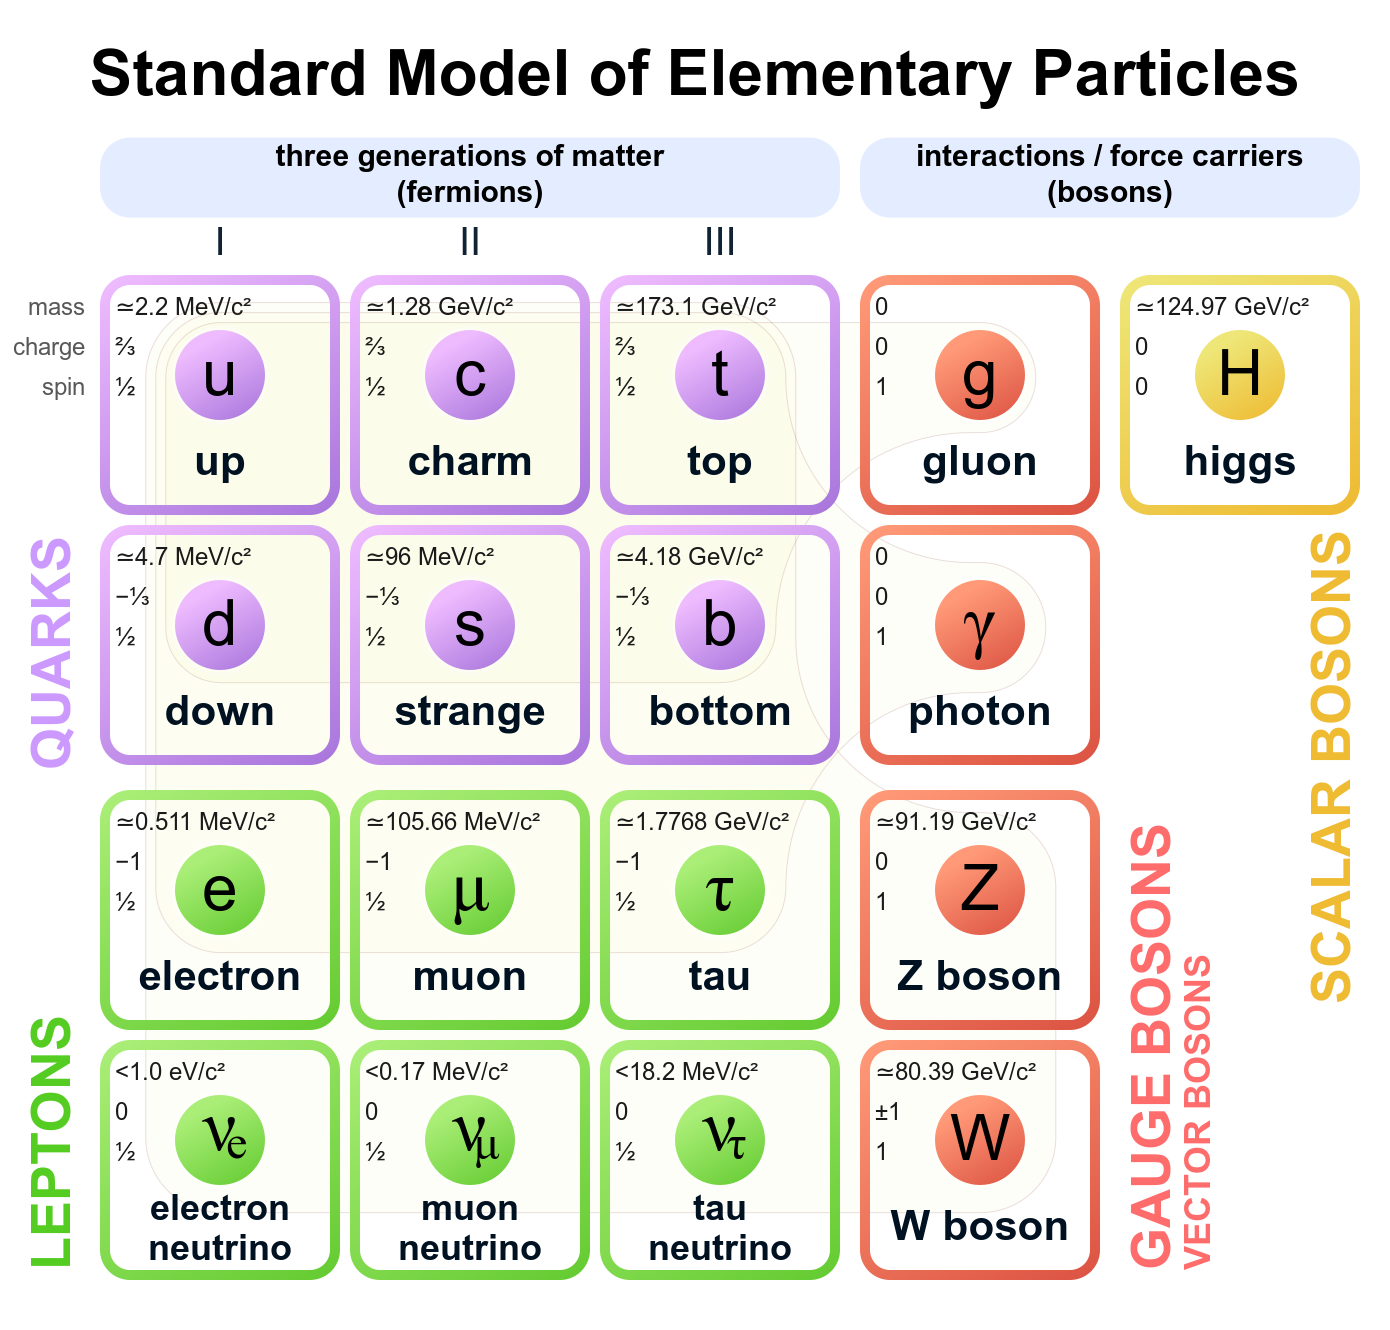
\includegraphics[width=0.8\textwidth]{plots/chapter2/sm_particles.png}
  \caption{Elementary particles of the SM.}
  \label{fig:sm_particles}
\end{figure}


\section{Theoretical building blocks}
The SM is a renormalizable QFT and has a $\suthree \times \sutwo \times \uone$ symmetry structure. The group theory aims to understand the general, abstract details of structures. The Lagrangian describes the dynamics of a system. A type of QFT is a gauge theory, where gauge fields require symmetry under local transformations. In the following paragraphs, a brief overview of groups and Lagrangian is given, and their application in a QFT is described.

A group is a set, G, together with an operation $\star$ that combines any two elements $a$ and $b$ to form another element, denoted $a \star b$. The set and operation, (G, $\star$), must satisfy four requirements to qualify as a group: closure, associativity, the existence of an identity element, and an inverse element. A group is Abelian if the group's elements commute under the group operation $(a \star b = b \star a)$. If the elements do not commute, the group is called non-Abelian. The number of elements in the group determines the order $n$ of the group. A group can be represented in terms of $n \times n$ matrices.

Lie groups are a special type of groups that are parameterized by one or more continuous variables. The transformation of elements in Lie groups can be described as matrices M. These matrices are unitary if the Hermitian conjugate is also the inverse of the transformation, $\text{M}^{\dagger}=(\text{M}^{*})^{\text{T}}=\text{M}^{-1}$. A unitary group is a set of such $n \times n$ matrices that preserve the norm under transformations and correspondingly the probability amplitude. If the unitary matrix's determinant is $\operatorname{det}|\text{M}|=1$, then the volume is preserved under such transformations. A set of such matrices form the special unitary group $\text{SU}(n)$.

The Lagrangian gives the information about the dynamics of a system as a function of generalized coordinates $q$ and their time derivatives $\dot{q}$. In classical physics, the Lagrangian is defined as the kinetic energy minus the potential energy $L=T(q, \dot{q})-V(q)$. In a field theory, the Lagrangian is replaced by the Lagrangian density $\mathcal{L}$, which is a function of the fields $\phi(x^{\Pgm})$, which are functions of spacetime and their derivatives $\partial_{\mu} \phi$. The action $S$ of the system is defined as $S=\int \text{d}^{4} x \mathcal{L}$.

In quantum mechanics, space is treated as an operator, and time is treated as a parameter. In a relativistic theory, space and time have to be treated on an equal footing. QFT interprets the fields as operators parameterized by the spacetime coordinates. It is impossible to measure both the field and its time rate of change simultaneously to infinite precision at a given spacetime point. The vacuum is the state with the lowest possible energy level. When a field operator acts on the vacuum, it produces a state with some energy.

The Lorentz group is the group of all Lorentz transformations of Minkowski spacetime. The Lorentz group contains two copies of the SU(2) group, where the SU(2) group represents spin. The spin of the particle $j$ characterizes the different representations. The Lorentz group can be represented by $(j, j^{\prime})$ for each of the two SU(2) subgroups. There are three important representations of the Lorentz group:

\begin{itemize}
\item The $(0, 0)$ scalar representation.
\item The $(\frac{1}{2}, 0) \oplus(0, \frac{1}{2} )$ left-handed/right-handed spinor representations.
\item The $(\frac{1}{2}, \frac{1}{2} )$ vector representation.
\end{itemize}

Spin is a rotation in the spinor space of SU(2). The spin-0 fields are called scalar fields. Complex scalar fields have the form $\phi = \phi_{1} + i \phi_{2}$, with two real degrees of freedom and hence the fields $\phi$ and $\phi^{\dagger}$ are treated independently.

The spin-1/2 fields are called spinor fields $\Psi$. The left-handed $\Psi_{L}$ and right-handed $\Psi_{R}$ spinors transform the same under rotations but differently under boosts. The adjoint spinor $\bar{\Psi}=\Psi^{\dagger} \gamma^{0}$ has to be defined to have Lorentz invariant terms in the Lagrangian density. The matrices satisfy the anti-commutation relation (Clifford algebra):
%
\[ \left\{\gamma^{\mu}, \gamma^{\nu}\right\}=\gamma^{\mu} \gamma^{\nu}+\gamma^{\nu} \gamma^{\mu}=-2 \eta^{\mu \nu} \mathbb{1} \]
%
with Minkowski metric $\eta^{\mu \nu}$.

A particular type of Lorentz transformations called Parity transformations $\Lambda_{P}$ switches the coordinate frame's handedness. Under parity transformations, left-handed spinors are transformed into right-handed spinors. To be Lorentz invariant, the adjoint field of a left-handed spinor field should be the same as the right-handed spinor field $\bar{\Psi}_{L}=\Psi_{R}$ and vice versa. The field can be projected onto the left and right-handed components using the projection operators: $P_{+} \Psi=\Psi_{R}$ and $P_{-} \Psi=\Psi_{L}$. The charge conjugation is another important transformation: $\Psi \to C \bar{\Psi}^{T}=-i \gamma^2 \Psi^{*}$, which swaps the charge of the field.

The spin-1 fields are called vector fields \amu. Under Lorentz transformations the four components of the vector fields transform as a spacetime vector. The Lorentz invariant terms are:

\begin{equation}
  \amu \text{A}^{\mu}, \quad (\partial_{\mu} \text{A}_{\nu})(\partial^{\mu} \text{A}^{\nu}), \quad (\partial_{\mu} \text{A}^{\mu})(\partial_{\nu} \text{A}^{\nu})
\end{equation}

In QFT, the fundamental fermions are represented as spinor fields, while the gauge bosons are represented as vector fields. An interaction term in the combined Lagrangian densities of both fields leads the two fields to interact. Such a term can be introduced using gauge theory.

Gauge theories are theories in which the Lagrangian is invariant under a continuous group of local transformations with a spacetime dependence. The possible transformations are associated with a Lie group. The elements of a group can be expressed in terms of the group generators. The Lagrangian density of a fermion field is defined to satisfy the Dirac equation. To make the Lagrangian density invariant under a local gauge transformation, a new vector field \amu has to be introduced for each group generator. The vector field can be expressed in terms of the group generators, $\amu=\amu^{a} \ta$, and the gauge bosons are the quanta of these fields.

The derivative $\partial_{\mu}$ in the Lagrangian density is replaced by the covariant derivative $D_{\mu}$, which is $\partial_{\mu}$ along with a term proportional to a gauge field. The second term of the covariant derivative introduces the interaction terms. The vector field dynamics can be included with a kinetic term proportional to the fields' derivatives. The local gauge symmetry is broken if the Lagrangian has terms proportional to $\amu \text{A}^{\mu}$, hence the vector fields are required to be massless. The general principle of local gauge invariance can be used to derive all fundamental interactions of the SM. In the SM, the \PW and \PZ bosons acquire their mass through the Higgs mechanism, which combines the principles of gauge theory and spontaneous symmetry breaking.

When a local symmetry is broken, the gauge fields can acquire mass. A global symmetry that is broken results in massless bosons called Goldstone bosons~\cite{Goldstone:1961eq, Goldstone:1962es}. If we consider a complex scalar field with a Lagrangian that has a local \uone symmetry and a potential with the vacuum $V_{\text{minimum}}$, then choosing a particular ground state breaks the system's symmetry and is considered ``spontaneous'' because there are no external means by which this occurs. After a change of basis, the field is expanded around the constant vacuum value, writing the fields in terms of fluctuations around the chosen vacuum. We can choose the vacuum for a local U(1) symmetry so that the vacuum is real and that $\phi$ is always real; therefore, $\phi$ can be expanded as $\phi = v + \text{H}$, with H being a real scalar field. When a local \uone symmetry is broken, it results in a real scalar with a mass, and the field \amu, originating from the local gauge symmetry, acquires mass.


\section{The Standard Model}
The SM is a non-Abelian gauge theory based on the group $\col \times \iso \times \hyp$, where C stands for color, L indicates that the interaction only involves left-handed states, and Y stands for the hypercharge. The transformations in the color space are represented by the group \col and described by QCD. QCD describes the strong interaction mediated by eight gauge bosons ($\gmu^{a}$) called gluons. Quarks are described as a triplet of spinors that differ in color (red, blue, or green).

\begin{equation}
  \begin{array}{|l|l|c|c|}
    \hline \text { Group } & \text { Operation } & \text { Coupling } & \text { Vector field } \\
    \hline \hyp & \text { Phase } & g^{\prime} & \bmu \\
    \hline \iso & \text { Weak isospin } & g & \wmu^{a} \\
    \hline \col & \text { Color } & g_{S} & \gmu^{a} \\
    \hline
  \end{array}
  \label{tab:group}
\end{equation}

The electroweak theory is represented by the group $\iso \times \hyp$. The neutrinos only interact via the weak interaction, which is represented by \iso. As only left-handed fields interact under \iso, only a left-handed neutrino is needed. The left-handed and right-handed fields can interact under the \hyp group, therefore charged leptons have to exist in both a left-handed and a right-handed state. Left-handed doublet fields
%
\begin{equation}
  \psi_{L}=\left(\begin{array}{l}
  \nu_{e} \\
  e_{L}
  \end{array}\right)
\end{equation}
%
and right-handed singlet fields $e_{R}$ are introduced. The group \iso has three associated gauge fields $\wmu^{a}$ and the group \hyp has one gauge field \bmu. The symmetry groups, couplings, and the associated vector fields are summarized in Table~\ref{tab:group}.

The Higgs field is a complex scalar $\iso \times \hyp$ doublet field. The Higgs boson is a spin-0 particle and is the field quanta of the Higgs field. The Higgs boson's fundamental vertices with the fermions, the gauge bosons of the weak interaction, and its self-interactions can be seen in Figure~\ref{fig:h_vertices}. The Higgs mechanism breaks the electroweak theory into two separate forces: the broken weak theory and the unbroken theory of electromagnetism associated with the $\uone_{em}$ symmetry of QED. The resulting fields $\amu, \wmu^{\pm}$, and $\zmu^{0}$ are linear combinations of the vector fields of $\iso \times \hyp$:
%
\begin{equation}
  \begin{aligned}
    \amu&=\sin \theta_{W} \wmu^{3}+\cos \theta_{W} \bmu \\
    \wmu^{\pm}&=(\wmu^{1} \mp i \wmu^2) / \sqrt{2} \\
    \zmu^{0}&=-\cos \theta_{W} \wmu^{3}+\sin \theta_{W} \bmu
  \end{aligned}
\end{equation}
%
with the weak mixing angle $\theta_{W}=\tan ^{-1}(\frac{g^{\prime}}{g})$, $\sin \theta_{W}=g^{\prime} / \sqrt{g^2+g^{\prime 2}}$ and $\cos \theta_{W}=g / \sqrt{g^2+g^{\prime 2}}$ written in terms of the couplings $g$ of \iso and  $g^{\prime}$ of \hyp. The weak mixing angle relates the strength of the weak and electromagnetic interaction. Furthermore, the electromagnetic coupling $e$ of $\uone_{em}$ is given by $e \equiv g \sin \theta_{W}$.

\begin{figure}[htbp]
  \centering
  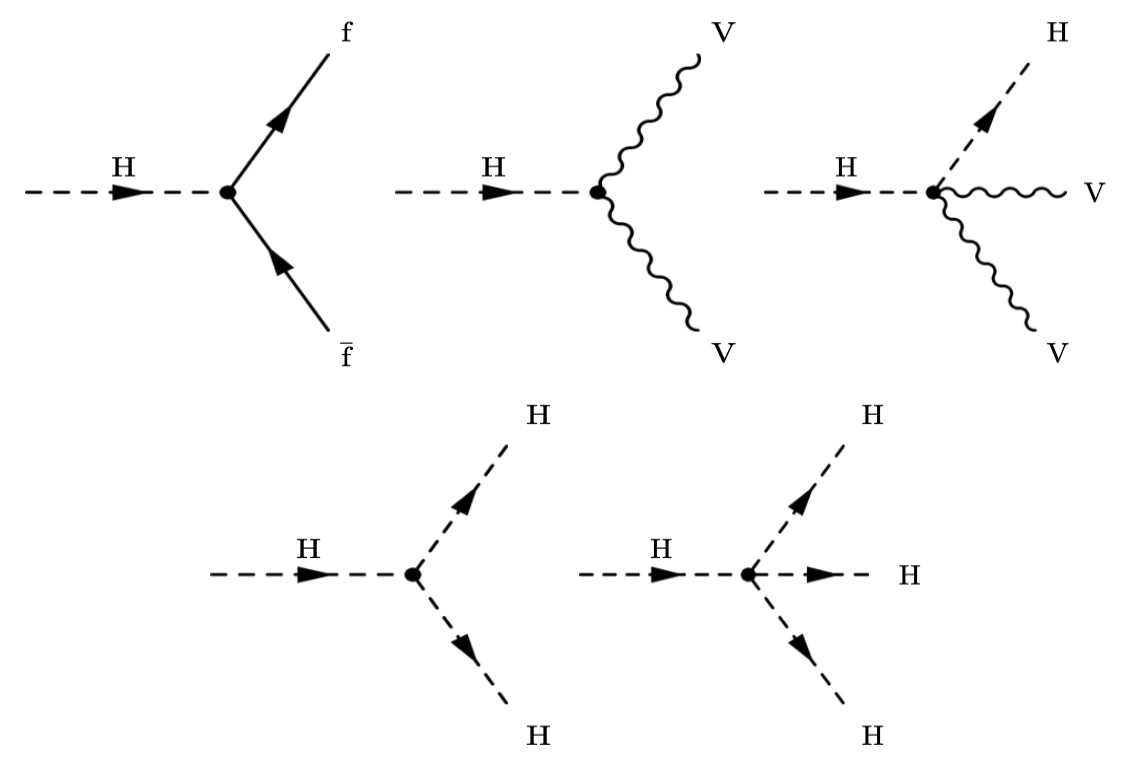
\includegraphics[width=0.8\textwidth]{plots/chapter2/h_vertices.png}
  \caption{Fundamental vertices of the Higgs boson. Fermions are denoted $\text{f}$, anti-fermions are denoted $\bar{\text{f}}$, and gauge bosons of the weak interaction are denoted $\text{V}$.}
  \label{fig:h_vertices}
\end{figure}

\subsection{Electroweak symmetry breaking and the Higgs boson}
For the Higgs mechanism, an arbitrary scalar potential
%
\begin{equation}
  V(\Phi)=\mu^2 \Phi^{\dagger} \Phi+\lambda(\Phi^{\dagger} \Phi)^2
\end{equation}
%
with a self-interacting scalar doublet field $\Phi$ is introduced. The term with the coefficient $\mu^2$ is the mass term of the field. The scalar doublet field $\Phi$ has four degrees of freedom, which are the CP-even and CP-odd components $\phi^{0}$ and $a^{0}$, and the complex charged component $\phi^{+}$:

\begin{equation}
  \Phi=\frac{1}{\sqrt{2}}\left(
  \begin{array}{c}
    \sqrt{2} \phi^{+} \\
    \phi^{0}+i a^{0}
  \end{array}\right)
\end{equation}

For $\mu^2<0$, the scalar doublet field's neutral component acquires a non-zero vacuum expectation value (VEV). Then $\phi^{0}$ can be expanded as $\phi^{0} = v + \text{H}$ with:

\begin{equation}
  \Phi=\frac{1}{\sqrt{2}}\left(
  \begin{array}{c}
    0 \\
    v + \text{H}
  \end{array}\right)
\end{equation}

After electroweak symmetry breaking, the $\col \times \iso \times \hyp$ is broken into a $\col \times \uone_{\text{em}}$. There are three massless Goldstone bosons, which can be identified with three degrees of freedom of the Higgs field. The covariant derivative in the kinematic term couples the Higgs field to the $\wmu^{a}$ and \bmu fields. Thus, the Goldstone bosons mix with the gauge bosons of the corresponding generators of broken symmetries, and the physical \PW and \PZ gauge bosons acquire masses:

\begin{equation}
  \text{M}_{\text{W}}^2=\frac{g^2 v^2}{4}, \quad \text{M}_{\text{Z}}^2=\frac{(g^{\prime 2}+g^2) v^2}{4}
\end{equation}

After electroweak symmetry breaking, there is one remaining degree of freedom of the Higgs field, which is the Higgs boson. The mass of this new scalar particle is given by $\mh = \sqrt{2 \lambda} v$, where $\lambda$ is the self-coupling parameter. One crucial aspect of the electroweak symmetry breaking is the sign of $\mu^2=-\lambda v^2$. The expectation value of the Higgs field is fixed by the Fermi coupling \gf: $v=(\sqrt{2} \gf)^{-1 / 2} \approx 246~\GeV$ which is measured very precisely in muon decays. In the SM, the fermions acquire mass through the Yukawa interactions between the Higgs field and the fermions. The charge conjugated Higgs doublet $\tilde{\Phi}$ is needed to allow interactions with up-type quarks. The Lagrangian of the Yukawa term is given by:
%
\begin{equation}
  \mathcal{L}_{\text {Yukawa }}=-\hat{\lambda}_{d_{i j}} \bar{q}_{L_{i}} \Phi d_{R_{j}}-\hat{\lambda}_{u_{i j} \bar{q}_{L_{i}}} \tilde{\Phi} d_{R_{j}}-\hat{\lambda}_{\ell_{i j}} \bar{\ell}_{L_{i}} \Phi e_{R_{j}}+\text {h.c.}
\end{equation}
%
where $\hat{\lambda}$ are $3 \times 3$ coupling coefficient matrices for the up and down-type quarks and the charged leptons. After electroweak symmetry breaking, the Higgs field acquires a VEV and the fermion mass eigenstate basis is chosen, so that the Higgs interactions are diagonalised: $\hat{\lambda}_{f_{i j}} \to \lambda_{f_{i}} \delta_{i j}$. The mass of the fermions is given by $\text{m}_{f_{i}} = \lambda_{f_{i}} v / \sqrt{2}$, with the corresponding Yukawa coupling $\lambda_{f}$. The Higgs boson was discovered by the ATLAS and CMS collaborations in 2012~\cite{Chatrchyan:2013lba}. Its mass and full width were measured to be $\mh = 125.09 \pm 0.24~\GeV$ and $\Gamma < 1.7~\GeV$.


\section{Lepton flavor violating decays of the Higgs boson}
The SM is considered to be an effective theory up to a certain scale $\Lambda$. The theoretical description of the SM does not incorporate the flavor structure. There are three main puzzles in the SM related to flavor~\cite{Raidal:2008jk}:
\begin{itemize}
  \item The reason for three generations of quarks and leptons.
  \item The principle underlying the formation of the Yukawa matrices describing the SM Yukawa interactions.
  \item The peculiar pattern of fermion masses and mixing.
\end{itemize}

The Yukawa interactions with the Higgs field gives charged leptons their mass. In the SM, LFV decays of the Higgs boson are forbidden because the Yukawa interaction matrix can be diagonalized in the mass basis. The SM extensions like multi-Higgs doublet models can introduce LFV Yukawa couplings along with additional CP-violation. These models can have tree-level Higgs mediated flavor changing neutral currents leading to LFV Yukawa couplings. Also, models like composite Higgs models~\cite{Blankenburg:2012ex} and models with extra dimensions can introduce LFV Yukawa couplings.

A direct mass term of the charged leptons is not gauge invariant, but interactions of the charged leptons to the scalar Higgs field can be introduced with the following term in the Lagrangian:
%
\begin{equation}
  \mathcal{L}_{\text{SM}}=-\lambda_{i j} \overline{L_{L}}^{i} \Phi \ell_{R}^{j}+ \text{h.c.}
\end{equation}
%
where with $\bar{L}_{L}^{i}=(\bar{\nu}_{\ell}^{i}, \bar{\ell}_{L}^{i})$, are the \iso doublets, and $\ell_{R}^{i}$ are the weak singlets with the indices $i, j$ running over generations. After electroweak symmetry breaking, the Higgs doublet can be written in terms of the VEV and the physical Higgs boson leading to the following Lagrangian:
%
\begin{equation}
  \begin{aligned}
    \mathcal{L}_{\text{SM}} &=-\frac{\lambda_{i j}}{\sqrt{2}}(v + \text{H}) \overline{\ell_{L}}^{i} \ell_{R}^{j}+ \text{h.c.} \\
    &=-\frac{\lambda_{i j}}{\sqrt{2}} v \overline{\ell_{L}}^{i} \ell_{R}^{j} - \frac{\lambda_{i j}}{\sqrt{2}} \overline{\ell_{L}}^{i} \ell_{R}^{j} \text{H} + \text{h.c.}
  \end{aligned}
\end{equation}
%
where the term proportional to $\bar{\ell}_{L}^{i} \ell_{R}^{j}$ is the mass term of the charged leptons and the term proportional to $\bar{\ell}_{L}^{i} \ell_{R}^{j} \text{H}$ describes the Yukawa interactions. The mass matrix m, with $\text{m}_{ij}=\frac{\lambda_{ij}}{\sqrt{2}} v$, can be diagonalised using the matrices $V_{L}$ and $V_{R}$:
%
\begin{equation}
  \text{m} = \left(\begin{array}{ccc}
  \text{m}_{e} & 0 & 0 \\
  0 & \text{m}_{\Pgm} & 0 \\
  0 & 0 & \text{m}_{\Pgt}
  \end{array}\right)=\frac{1}{\sqrt{2}} V_{L} \lambda V_{R}^{\dagger} v=\frac{\lambda^{\text{m}}}{\sqrt{2}} v
\end{equation}
%
where $\lambda^{\text{m}}=V_{L} \lambda V_{R}^{\dagger}$ is written in terms of the mass basis. The Yukawa interaction matrix can also be written in terms of the mass basis:
%
\begin{equation}
  \text{Y}=V_{L} \frac{\lambda}{\sqrt{2}} V_{R}^{\dagger}=\frac{\lambda^{\text{m}}}{\sqrt{2}}=\frac{\text{m}}{v}=\left(\begin{array}{ccc}
  \Yee & 0 & 0 \\
  0 & \Ymm & 0 \\
  0 & 0 & \Ytt
  \end{array}\right)
\end{equation}
%
which is also diagonal. Thus, there are no LFV Yukawa interactions in the SM.

\textbf{Dimension-6 operators:} Assuming that the Higgs field is the only field that causes electroweak symmetry breaking and that the particle spectrum is only composed of the SM particles up to an energy scale $\Lambda \gg 200~\GeV$, we can integrate out the additional heavy fields, which gives us an effective field theory. The SM Lagrangian, which has dimension four, can be extended with higher-dimension operators. An effective Lagrangian with additional dimension-6 operators $O_{n}^{i j}$ can be written as:
%
\begin{equation}
  \mathcal{L}_{\text{eff}}=\mathcal{L}_{\text{SM}}+\sum_{\text{n}ij} \frac{\alpha_{\text{n}}^{ij}}{\Lambda^2} O_{\text{n}}^{i j}
\end{equation}
%
where $i, j$ denote flavor indices, n runs over the number of independent operators, $\Lambda$ is the scale of new physics, and $\alpha_{\text{n}}^{i j}$ are coefficients~\cite{DiazCruz:1999xe}.

The effects of new physics at the electroweak scale can be described in a model-independent way using this effective Lagrangian. The effective Lagrangian can also contain a dimension-5 operator, which can generate neutrino masses, but it cannot generate LFV interactions for the Higgs boson. However, LFV interactions of the Higgs boson can be generated using the dimension-6 operator $O_{L \phi}^{i j}=(\Phi^{\dagger} \Phi)(\bar{L}_{i} \ell_{R j} \Phi)$ which is a Yukawa-type operator. The dimension-6 operator also contributes to the fermion mass matrices. After including these contributions in the fermion mass matrices, which are then diagonalized and the interaction term of the Lagrangian is written in terms of the mass basis. The Lagrangian has the following additional term after including the Yukawa-type operator:
%
\begin{equation}
  \Delta \mathcal{L}=-\frac{\lambda_{i j}^{\prime}}{\Lambda^2}(\Phi^{\dagger} \Phi)(\bar{L}_{L}^{i} \ell_{R}^{j} \Phi)+h.c.
\end{equation}
%
where $\lambda_{i j}^{\prime}$ is the coefficient $\alpha_{n}^{i j}$ of the dimension-6 operator $O_{L \phi}^{i j}$.

Electroweak symmetry breaking leads to the following Lagrangian terms:
%
\begin{equation}
  \begin{aligned}
    \Delta \mathcal{L} &=-\frac{\lambda_{i j}^{\prime}}{\Lambda^2}(\frac{v+\text{H}}{\sqrt{2}})^2 \bar{\ell}_{L}^{i} \ell_{R}^{j}(\frac{v+\text{H}}{\sqrt{2}}) \\
    &=-\frac{\lambda_{i j}^{\prime}}{\Lambda^2} \frac{1}{(\sqrt{2})^{3}}(v^{3}+3 v^2 \text{H} + 3 v \text{H}^2 + \text{H}^{3}) \bar{\ell}_{L}^{i} \ell_{R}^{j} \\
    &=-\frac{1}{\sqrt{2}} \frac{\lambda_{i j}^{\prime}}{2 \Lambda^2}(v^{3} \overline{\ell_{L}^{i}} \ell_{R}^{j}+3 v^2 \overline{\ell_{L}^{i}} \ell_{R}^{j} \text{H} + 3 v \bar{\ell}_{L}^{i} \ell_{R}^{j} \text{H}^2+\bar{\ell}_{L}^{i} \ell_{R}^{j} \text{H}^{3})
  \end{aligned}
\end{equation}
%
where the term proportional to $\overline{\ell_{L}^{i}} \ell_{R}^{j}$ leads to an additional mass term of the charged leptons and the term proportional to $\overline{\ell_{L}^{i}} \ell_{R}^{j} \text{H}$ adds a further Yukawa-interaction term. Thus, the mass term of the effective Lagrangian is the sum of the SM mass term and the additional contribution:

\begin{equation}
  \begin{aligned}
    \mathcal{L}_{\text {mass }} &=\mathcal{L}_{\text {mass}, \text{SM}}+\Delta \mathcal{L}_{\text {mass }} \\
    &=-(\frac{\lambda_{i j}}{\sqrt{2}} v+\frac{1}{\sqrt{2}} \frac{\lambda_{i j}^{\prime}}{2 \Lambda^2} v^{3}) \bar{\ell}_{L}^{i} \ell_{R}^{j} \\
    &=-\frac{1}{\sqrt{2}}(\lambda_{i j}+\frac{v^2}{2 \Lambda^2} \lambda_{i j}^{\prime}) v \bar{\ell}_{L}^{i} \ell_{R}^{j}
  \end{aligned}
\end{equation}

The term of the effective Lagrangian which describes the Yukawa interactions is given by:

\begin{equation}
  \begin{aligned}
    \mathcal{L}_{\text{Y}} &=\mathcal{L}_{\text{Y}, \text{SM}}+\Delta \mathcal{L}_{\text{Y}} \\
    &=-(\frac{\lambda_{i j}}{\sqrt{2}}+\frac{1}{\sqrt{2}} \frac{\lambda_{i j}^{\prime}}{2 \Lambda^2} 3 v^2) \bar{\ell}_{L}^{i} \ell_{R}^{j} \text{H} \\
    &=-\frac{1}{\sqrt{2}}(\lambda_{i j}+3 \frac{v^2}{2 \Lambda^2} \lambda_{i j}^{\prime}) \bar{\ell}_{L}^{i} \ell_{R}^{j} \text{H}
  \end{aligned}
\end{equation}

The mass matrix of the charged leptons can be diagonalized as for the SM using other matrices $V_{L}, V_{R}$:

\begin{equation}
  \sqrt{2} \text{m} = V_{L}[\lambda+\frac{v^2}{2 \Lambda^2} \lambda^{\prime}] V_{R}^{\dagger} v
\end{equation}

The Yukawa interaction matrix can then be written in terms of the mass basis:
%
\begin{equation}
  \begin{aligned}
    \sqrt{2} \text{Y} &=V_{L}[\lambda+3 \frac{v^2}{2 \Lambda^2} \lambda^{\prime}] V_{R}^{\dagger} \\
    &=\frac{\sqrt{2} \text{m}}{v}+V_{L} 2 \frac{v^2}{2 \Lambda^2} \lambda^{\prime} V_{R}^{\dagger} \\
    &=\frac{\sqrt{2} \text{m}}{v}+\frac{v^2}{\Lambda^2} V_{L} \lambda^{\prime} V_{R}^{\dagger} \\
    &=\frac{\sqrt{2} \text{m}}{v}+\frac{v^2}{\Lambda^2} \hat{\lambda}
  \end{aligned}
\end{equation}
%
where $\text{m}$ is the diagonal mass matrix and $\hat{\lambda}=V_{L} \lambda^{\prime} V_{R}^{\dagger}$. The first term is the Yukawa term of the SM, while the second term can introduce non-diagonal terms as $\hat{\lambda}$ is in principle an arbitrary non-diagonal matrix, leading to Yukawa couplings \Yij with possible LFV Yukawa interactions:

\begin{equation}
  \text{Y}_{i j}=\frac{\text{m}_{i}}{v} \delta_{i j}+\frac{v^2}{\sqrt{2} \Lambda^2} \hat{\lambda}_{i j}
\end{equation}

\textbf{Type-III 2HDM:} The two Higgs doublet model (2HDM) is one of the most studied extensions of the SM. The structure of Yukawa couplings can characterize them. In Type-I, Type-II, and Type-X 2HDM, each fermion type is coupled to only one scalar doublet. Thus there is no flavor violating Yukawa couplings of the neutral scalar boson in this case. In Type-III 2HDM, however, both of the scalar doublets couple to all the fermions. As a result, there is a possibility of flavor violation in the neutral scalars Yukawa couplings~\cite{Primulando:2016eod}.

In the Higgs basis, the VEV resides only in $\Phi_{1}$ and the fields $\Phi_{1}$ and $\Phi_{2}$ can be expanded as
%
\begin{equation}
  \Phi_{1}=\left(\begin{array}{c} \text{G}^{+} \\ \frac{1}{\sqrt{2}}\left(v+\phi_{1}+i \text{G}^{0}\right) \end{array}\right), \quad
  \Phi_{2}=\left(\begin{array}{c} \text{H}^{+} \\ \frac{1}{\sqrt{2}}\left(\phi_{2}+i \text{A}\right) \end{array}\right)
\end{equation}
%
where $v$ is the VEV, $\text{G}^{\pm}$ and $\text{G}^0$ are the would-be Goldstone bosons, $\text{H}^{\pm}$ is the charged Higgs, A is the neutral CP-odd Higgs, $\phi_{1}$ and $\phi_{2}$ are the neutral CP-even Higgs. The fields $\phi_{1}$ and $\phi_{2}$ are not mass eigenstates. They are related to the mass eigenstates H (SM Higgs boson) and $\text{H}^{'}$ (neutral heavy Higgs boson) by

\begin{equation}
  \left(\begin{array}{l} \phi_{1} \\ \phi_{2} \end{array}\right) = \left(\begin{array}{r} \cos \alpha \quad \sin \alpha \\ -\sin \alpha \quad \cos \alpha \end{array}\right)\left(\begin{array}{l} \text{H} \\ \text{H}^{'} \end{array}\right)
\end{equation}

The Yukawa sector in the Type-III 2HDM is given by
%
\begin{equation}
  \mathcal{L}_{\text{Yukawa}}=-\frac{\sqrt{2} \text{m}_{\ell}^{i}}{v} \delta^{i j} \bar{L}_{L}^{i} \ell_{R}^{j} \Phi_{1}-\sqrt{2} \text{Y}_{\ell}^{i j} \bar{L}_{L}^{i} \ell_{R}^{j} \Phi_{2}
\end{equation}
%
where $\text{m}_{\ell}$ are lepton masses, $\text{Y}_{\ell}$ are the Yukawa coupling matrices, and the indices $i, j, k$ run over lepton families. After electroweak symmetry breaking, the Yukawa couplings in the physical basis read

\begin{equation}
  \begin{aligned}
    \mathcal{L}_{\text{Yukawa}} &\supset -y_{\ell, \text{H}}^{i j} \bar{\ell}_{L}^{i} \ell_{R}^{j} \text{H} - y_{\ell, \text{H}^{'}}^{i j} \bar{\ell}_{L}^{i} \ell_{R}^{j} \text{H}^{'} + \text{h.c.} \\
    y_{\ell, \text{H}}^{i j} &=\frac{\text{m}_{\ell}^{i}}{v} \delta^{i j} \cos \alpha - \text{Y}_{\ell}^{i j} \sin \alpha \\
    y_{\ell, \text{H}^{'}}^{i j} &=\frac{\text{m}_{\ell}^{i}}{v} \delta^{i j} \sin \alpha + \text{Y}_{\ell}^{i j} \cos \alpha
  \end{aligned}
\end{equation}

\textbf{LFV Yukawa couplings:} The inclusion of LFV Yukawa interactions were discussed by introducing a dimension-6 operator to the Lagrangian and in theories with more than one Higgs doublet, where the scalar fields can mix. There are several possible additional terms to the Lagrangian due to new physics, which prevent the simultaneous diagonalization of mass matrix and the Yukawa matrix. Thus, the Yukawa term of the Lagrangian for the charged leptons in the mass basis is after the electroweak symmetry breaking in general given by:
%
\begin{equation}
  \mathcal{L}_{\text{Yukawa}} = -\text{m}_{i} \bar{\ell}_{L}^{i} \ell_{R}^{i} - \text{Y}_{i j} \bar{\ell}_{L}^{i} \ell_{R}^{j} \text{H}+\text{h.c.}
\end{equation}
%
where \Yij are the entries of the Yukawa matrix:
%
\begin{equation}
  \text{Y}=\left(\begin{array}{ccc}
  \Yee & \Yem & \Yet \\
  \Yme & \Ymm & \Ymt \\
  \Yte & \Ytm & \Ytt
  \end{array}\right)
\end{equation}
%
which can have LFV Yukawa couplings \Yij. LFV Yukawa couplings allow LFV decays of the Higgs boson.

The Higgs boson couples to all particles according to their mass in the SM. The LFV Yukawa couplings might be related closely to the fermion mass matrices in the presence of new physics, reflecting the observed fermion mass hierarchy~\cite{Cheng:1987rs}. The LFV couplings then have a hierarchical structure given by $\Delta_{ij} \sqrt{\text{m}_{i} \text{m}_{j}}$, where $i, j$ are the generation indices, and $\Delta_{ij}$ is related to the mass mixing. The mass corrections to the lepton masses coming from mass mixing are assumed to be small in the natural assumption. The SM Yukawa couplings are taken for the flavor diagonal couplings. The LFV branching fractions can be expressed in terms of the SM ones:
%
\begin{equation}
  \BHij = \BHsm \cdot \frac{\text{m}_{\ell_{j}}}{\text{m}_{\ell_{i}}}
\end{equation}
%
with the total decay width asummed to be the SM one, \BHij being the natural branching fraction and \BHsm being the branching fraction for the SM Higgs boson decay to two leptons. The LFV branching fractions are expected to be of similar size or smaller than \BHij. A naturalness assumption referred to as theoretical naturalness limit can also be derived for the Yukawa couplings:

\begin{equation}
  |\Yji \Yij| \lesssim \frac{\text{m}_{i} \text{m}_{j}}{v^2}
\end{equation}


\section{Constraints from low-energy measurements}

Constraints on the Higgs boson's LFV decays have been derived using low-energy measurements and with certain assumptions on the value of flavor diagonal Yukawa couplings. The constraints from several low-energy measurements on LFV Yukawa couplings are discussed in this section. These measurements and the assumptions used to derive constraints on the LFV Yukawa couplings are presented.

\textbf{Constraints from LFV decays \liljg:} LFV Yukawa couplings also contribute to LFV decays of the type \liljg, where $i, j$ are flavor indices with $i \neq j$. One-loop and two-loop diagrams of this process are shown in Figure~\ref{fig:tmg}. Constraints of the type $\sqrt{|\Yij|^2+|\Yji|^2}$ can be derived assuming SM values for \Ytt, \Ymm, and $\text{Y}_{\text{tt}}$. A further constraint on $(|\Ytm \Yet|^2 + |\Ymt \Yte|^2)^{1/4}$ can be obtained from $\Pgm \to \Pe \Pgg$ by setting \Yme and \Yem to zero.

\begin{figure}[htbp]
  \centering
  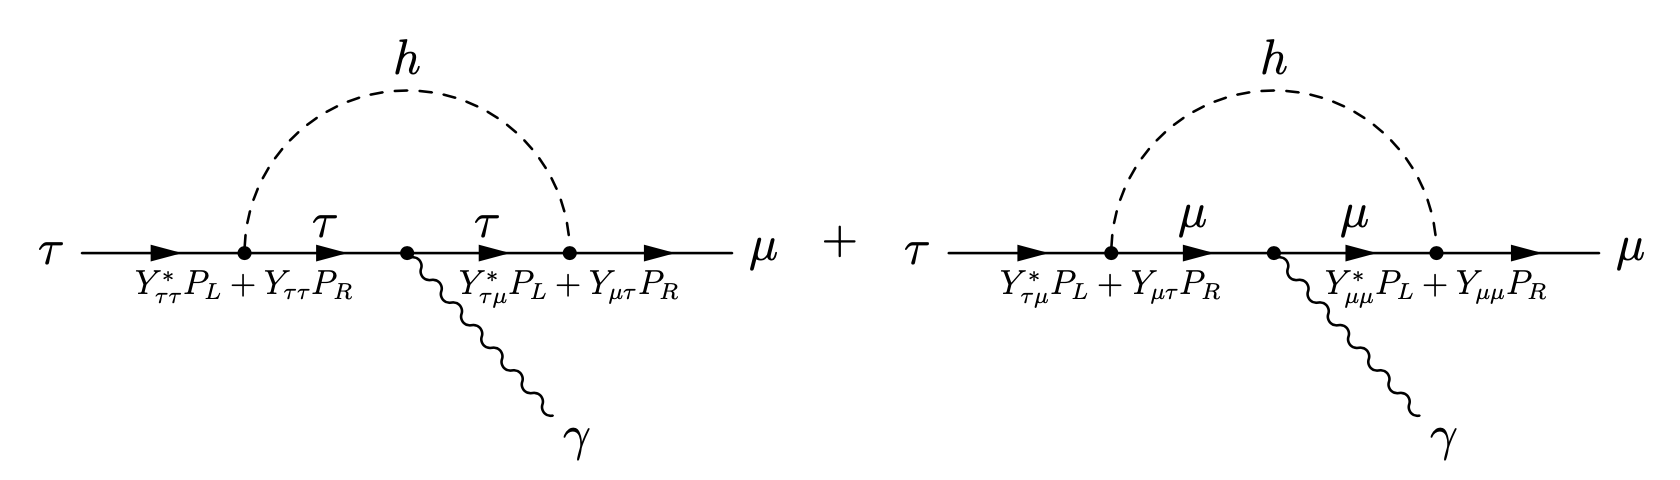
\includegraphics[width=0.8\textwidth]{plots/chapter2/1loop.png} \\
  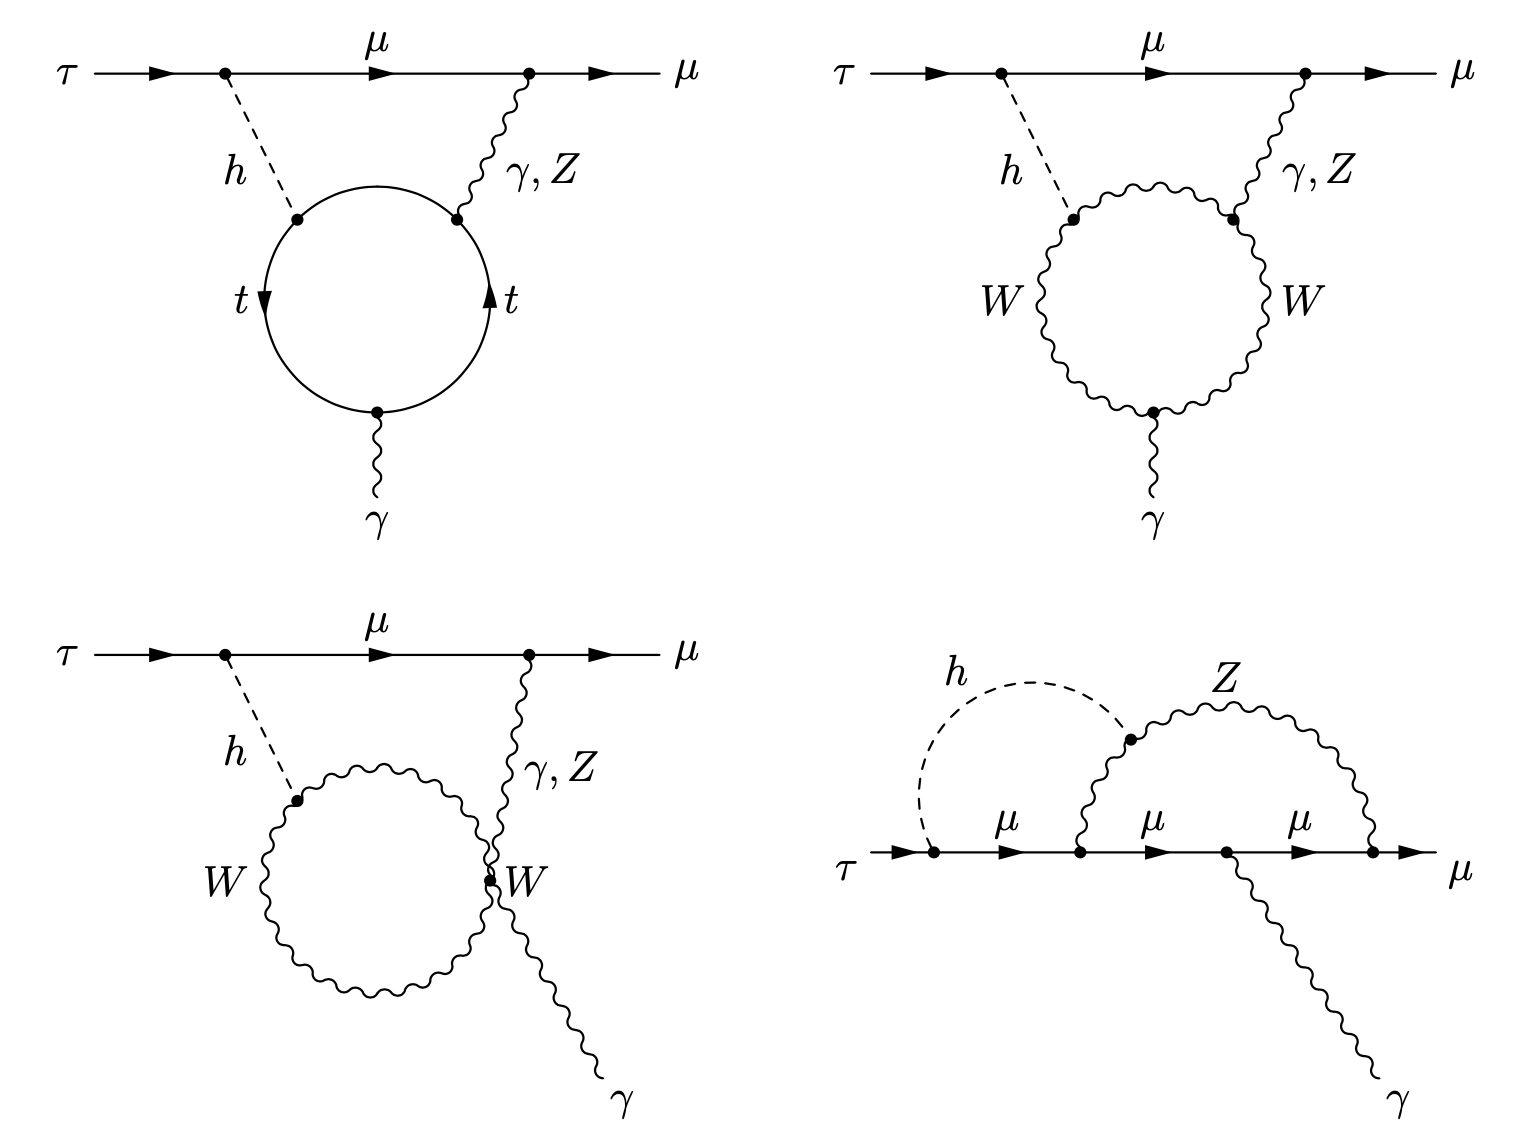
\includegraphics[width=0.8\textwidth]{plots/chapter2/2loop.png}
  \caption{Diagrams contributing to the flavor violating decay $\Pgt \to \Pgm \Pgg$, mediated by a Higgs boson with flavor violating Yukawa couplings.}
  \label{fig:tmg}
\end{figure}

\textbf{Constraints from LFV decays \ltl:} LFV Yukawa couplings also contribute to LFV decays of the type \ltl. Such decays have been searched for and constraints of the type $\sqrt{|\Yij|^2+|\Yji|^2}$ can be derived assuming SM values for \Ytt, \Ymm, and $\text{Y}_{\text{tt}}$. The \PZ boson contribution to the LFV decay $\Pgt \to \Pgm$ are neglected because their contributions are negligible~\cite{Goto:2015iha}.

\textbf{Constraints from muonium-antimuonium oscillations:} The muonium ($M$) bound state $\Pgm^{+} \Pe^{-}$ can oscillate to the antimuonium ($\bar{M}$) bound state $\Pe^{+} \Pgm^{-}$. An upper limit on the conversion probability $P(M \to \bar{M}) < 8.3 \times 10^{-11}$~\cite{Willmann:1998gd} was derived by the muonium-antimuonium conversion spectrometer experiment. The time-integrated conversion probability depends on the mass splitting between the two mass eigenstates of the mixed $M-\bar{M}$ system, which depends on $|\text{Y}_{\Pgm e}+\text{Y}_{e \Pgm}^{*}|$~\cite{Harnik:2012pb}.

\textbf{Constraints from magnetic and electric dipole moments:} The muon's experimental value $g_{\Pgm}-2$ is more than three standard deviations above the SM prediction. Neglecting terms suppressed by $\text{m}_{\Pgm} / \text{m}_{\Pgt}$ or $\text{m}_{\Pgt} / \text{m}_\text{H}$, the LFV contribution to $g_{\Pgm}-2$ due to the one-loop diagram has the form
%
\begin{equation}
  a_{\Pgm} \equiv \frac{g_{\Pgm}-2}{2} \propto \operatorname{Re}(\Ymt \Ytm)
\end{equation}
%
with the discrepancy between measurement and SM prediction having the size
%
\begin{equation}
  \Delta a_{\Pgm} \equiv a_{\Pgm}^{\text{exp}}-a_{\Pgm}^{\text{SM}}=(2.87 \pm 0.63 \pm 0.49) \times 10^{-9}
\end{equation}
%
where $a_{\Pgm}^{\text{exp}}$ and $a_{\Pgm}^{\text{SM}}$ are the measured and predicted value, respectively. The one-loop diagram can contribute to the muon's electric dipole moment if the LFV Yukawa couplings are complex. If the terms suppressed by $\text{m}_{\Pgm} / \text{m}_{\Pgt}$ or $\text{m}_{\Pgt} / \text{m}_\text{H}$ are neglected, the dependence on the LFV Yukawa couplings of the electric dipole moment $d_{\Pgm}$ is

\begin{equation}
  d_{\Pgm} \propto-\operatorname{Im}(\Ymt \Ytm)
\end{equation}

\textbf{Constraints from \mte conversion in nuclei:} LFV Yukawa couplings can also contribute to \mte conversion in nuclei via a tree-level exchange of the Higgs boson and one-loop diagrams with the Higgs boson and a photon exchange. The two-loop diagrams' contribution is larger than the one-loop diagrams because they are only suppressed by the weak gauge coupling or $\mathrm{Y_{tt}}$ and were taken into account for deriving the constraints on the LFV Yukawa couplings.

Constraints on the LFV Yukawa couplings from low-energy measurements are summarized in Table~\ref{tab:indirect}. The LFV decays of type \liljg give the strongest constraints. These measurements constrain the branching fractions of LFV Higgs boson decays to \mutau or \etau to be $\lesssim \mathcal{O}(10^{-1})$, while the constraint for the decay to \emm is stronger and calculated to be $\lesssim \mathcal{O}(10^{-8})$. Constraints on the branching fractions were derived under the assumption that only one of them contributes in addition to the SM Higgs boson's total width.

%%% Low energy constraints
\begin{table}[!hbpt]
\centering
\caption{Constraints on LFV Yukawa couplings from low-energy measurements ~\cite{Harnik:2012pb}.}
\begin{tabular}{ccc}
\hline
\hline
Channel                   & Coupling                   & Bound                 \\
\hline
$\Pgm \to \Pe \Pgg$       & $\sqrt{|\Yme|^2+|\Yem|^2}$ & $<3.6 \times 10^{-6}$ \\
$\Pgm \to 3 \Pe$          & $\sqrt{|\Yme|^2+|\Yem|^2}$ & $\lesssim 3.1 \times 10^{-5}$ \\
electron $g-2$            & Re(\Yem \Yme)              & $-0.019 \ldots 0.026$ \\
electron EDM              & $|Im(\Yem \Yme)|$          & $<9.8 \times 10^{-8}$ \\
$\Pgm \to$ \Pe conversion & $\sqrt{|\Yme|^2+|\Yem|^2}$ & $<1.2 \times 10^{-5}$ \\
$M-\bar{M}$ oscillations  & $|\Yme+\Yem^{*}|$          & $<0.079$ \\
\hline
$\Pgt \to \Pe \Pgg$       & $\sqrt{|\Yte|^2+|\Yet|^2}$ & $<0.014$ \\
$\Pgt \to 3 \Pe$          & $\sqrt{|\Yte|^2+|\Yet|^2}$ & $\leq 0.12$ \\
electron $g-2$            & Re(\Yet \Yte)              & $-2.1 \ldots 2.9 \times 10^{-3}$ \\
electron EDM              & $|Im(\Yet \Yte)|$          & $<1.1 \times 10^{-8}$ \\
\hline
$\Pgt \to \Pgm \Pgg$      & $\sqrt{|\Ytm|^2+|\Ymt|^2}$ & $<0.016$ \\
$\Pgt \to 3 \Pgm$         & $\sqrt{|\Ytm|^2+|\Ymt|^2}$ & $\lesssim 0.25$ \\
muon $g-2$                & Re(\Ymt \Ytm)              & $(2.7 \pm 0.75) \times 10^{-3}$ \\
muon EDM                  & $|Im(\Ymt \Ytm)|$          & $-0.8 \ldots 1.0$ \\
\hline
$\Pgm \to \Pe \Pgg$       & $(|\Ytm \Yet|^2+|\Ymt \Yte|^2)^{1/4}$ & $<3.4 \times 10^{-4}$ \\
\hline
\hline
\end{tabular}
\label{tab:indirect}
\end{table}



\section{Lepton flavor violating decays of the Higgs boson at the LHC}

In the SM, the Higgs boson couples to all particles according to their mass. The branching fraction for Higgs boson decays to taus is in the order of 6\%, and the branching fraction of the Higgs boson to muons is in the order of 0.02\%. The LFV branching fractions are expected to be of the same size or smaller than \BHij using the natural assumption. Furthermore, LFV branching fractions \BHij can be expressed in terms of SM ones. Then, the LFV Higgs boson decay to \mutau should have a natural branching fraction in the order of 0.5\%, between decays to taus and muons. LFV decays of the Higgs boson to \etau would have a smaller natural branching fraction in the order of $0.001\% = 10^{-5}$.

Low-energy measurements indirectly constrain branching fractions of the LFV Higgs boson decays to \mutau or \etau to be smaller than 10\%, which is larger than their natural branching fractions. These constraints were derived, assuming flavor changing neutral currents to be dominated by Higgs boson contributions; therefore, LFV effects could be canceled by other new physics effects leading to weaker limits. Direct searches for LFV decays of the Higgs boson are independent of assumptions on other new physics models.

The CMS experiment published the first direct search for \Hmt~\cite{Khachatryan:2015kon}, followed by searches for \Het and \Hem decays~\cite{Khachatryan:2016rke}, using \pp collision data corresponding to an integrated luminosity of 19.7~\fb at a center-of-mass energy of 8~\TeV. A small excess of data with respect to the SM background-only hypothesis at $\mh = 125~\GeV$ was observed in the \Hmt channel, with a significance of 2.4 standard deviations, and the best fit for the branching fraction was found to be $\BHmt = (0.84^{+0.39}_{-0.37})\%$. A constraint was set on the observed (expected) branching fraction $\BHmt < 1.51\% (0.75\%)$ at 95\% CL. This search has improved the limit on the branching fraction \BHmt from the indirect limit by one order of magnitude.

No excess of events over the estimated background was observed in the \Het or \Hem channels, and observed (expected) upper limits on the branching fractions $\BHet < 0.69\% (0.75\%)$ and $\BHem < 0.035\% (0.048\%)$ at 95\% CL were set. The ATLAS Collaboration reported searches for \Het and \Hmt using \pp collision data at a center-of-mass energy of 8~\TeV, finding no significant excess of events over the background expectation, and set observed (expected) limits of $\BHmt < 1.43\% (1.01\%)$ and $\BHet < 1.04\% (1.21\%)$ at 95\% CL~\cite{Aad:2016blu, Aad:2015gha}.

The CMS experiment placed an upper limit on the observed (expected) branching fraction $\BHmt < 0.25\% (0.25\%)$ and $\BHet < 0.61\% (0.37\%)$ at 95\% CL using the 2016 dataset corresponding to an integrated luminosity of 35.9~\fb~\cite{Sirunyan:2017xzt}. The ATLAS experiment published the search results using the 2016 dataset corresponding to an integrated luminosity of 36.1~\fb and placed an upper limit of 0.28\% (0.37\%) and 0.47\% (0.34\%) on the \BHmt and \BHet with a 95\% CL, respectively~\cite{Aad:2019ugc}. Figure~\ref{fig:bh} shows the expected and observed 95\% CL upper limits for each category and their combination of the search performed by the CMS experiment. Figure~\ref{fig:yukawa} shows the corresponding Yukawa couplings.

\begin{figure}[htbp]
  \centering
  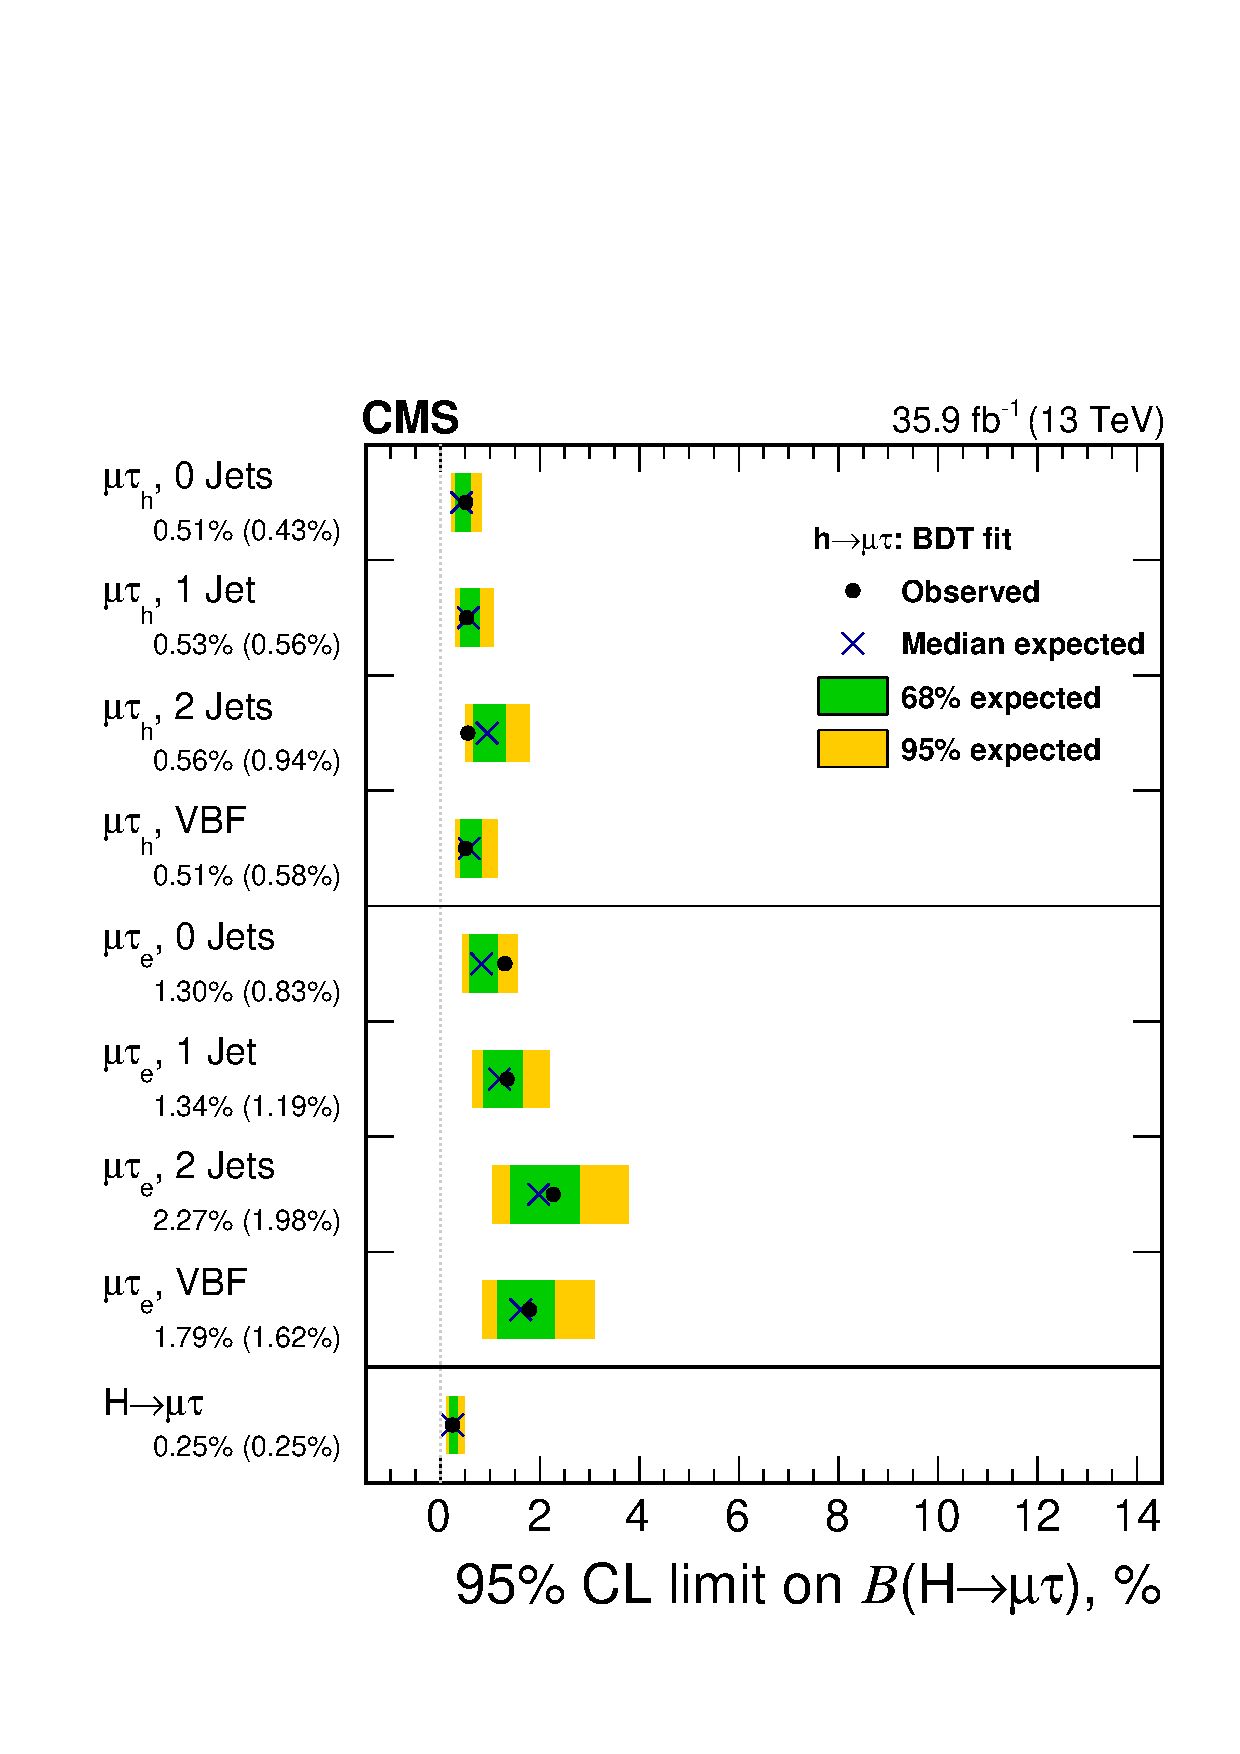
\includegraphics[width=0.45\textwidth]{plots/chapter2/BHmt.pdf}
  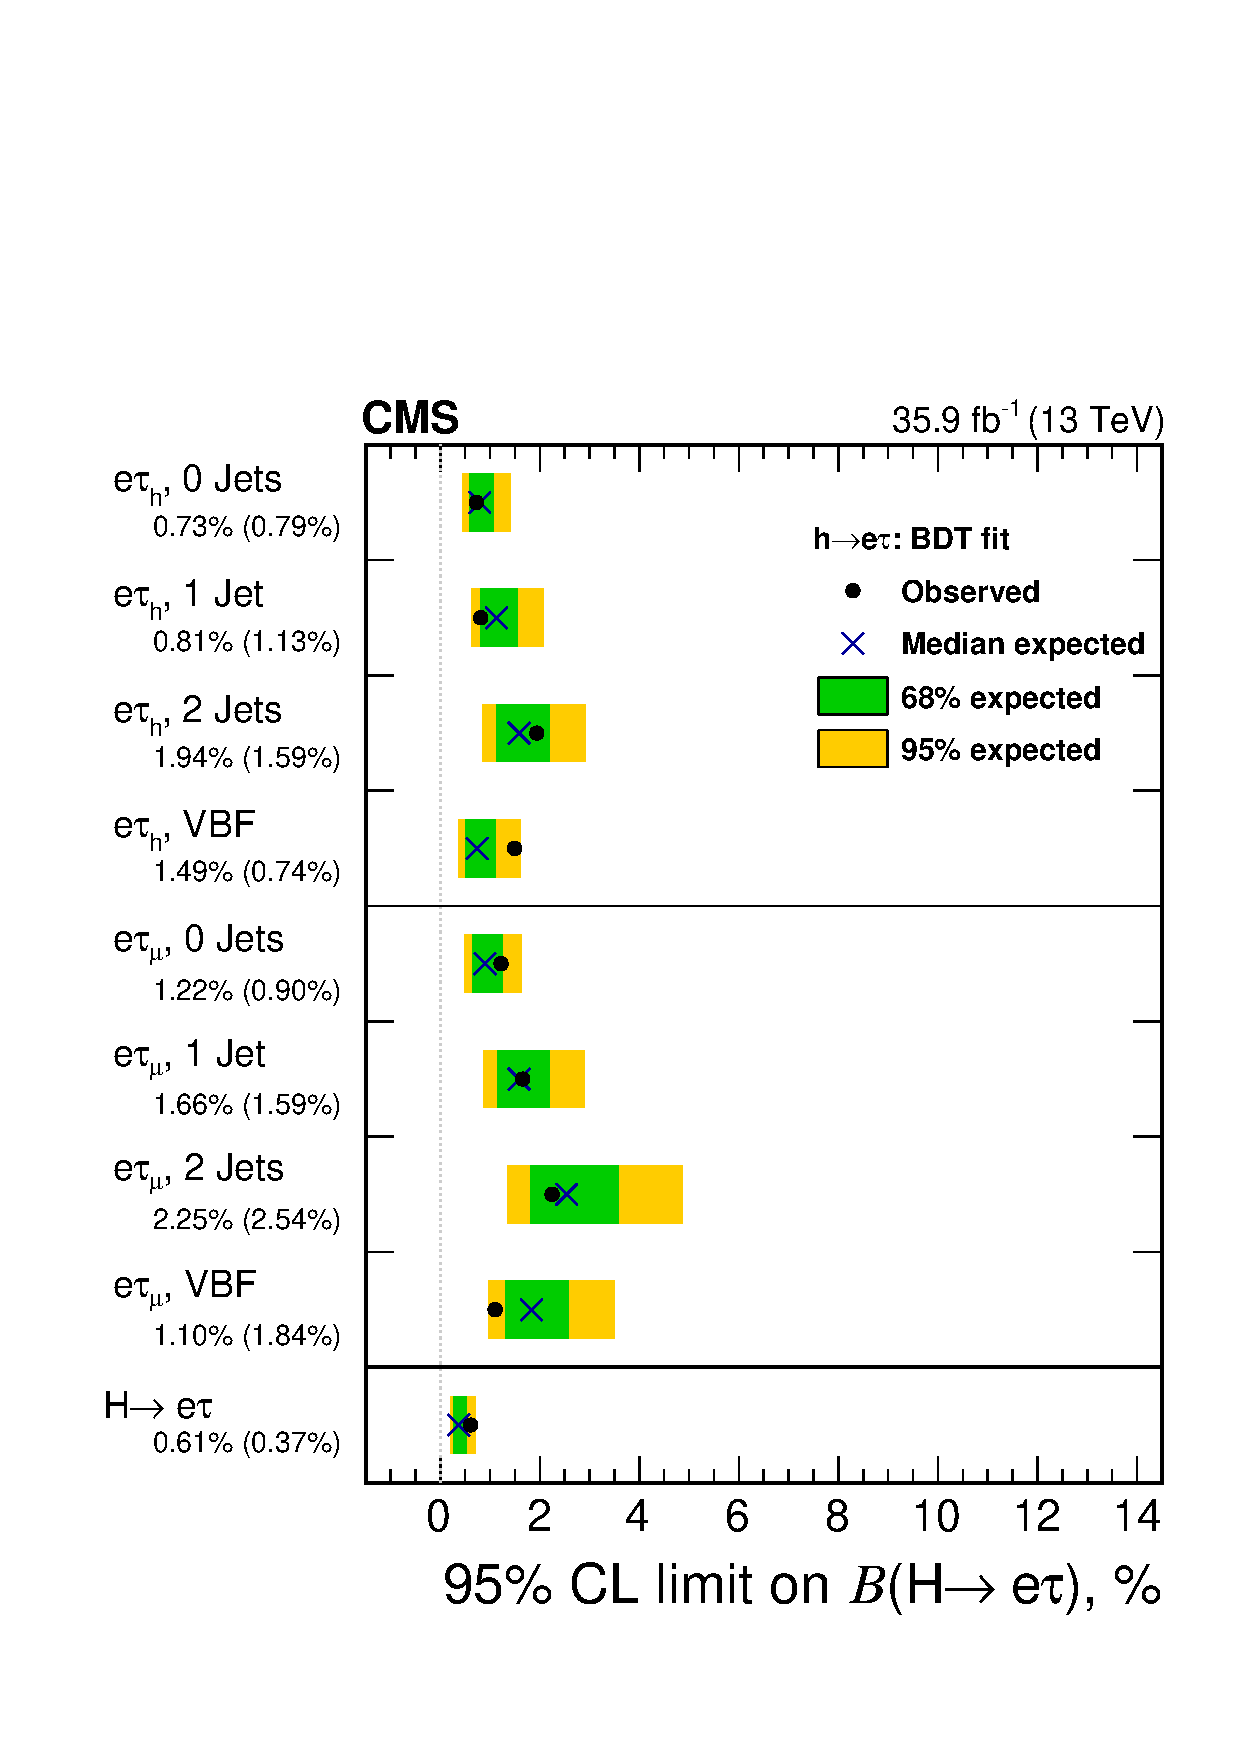
\includegraphics[width=0.45\textwidth]{plots/chapter2/BHet.pdf}
  \caption{Expected and observed 95\% CL upper limits for each category and their combination of the search performed by the CMS experiment~\cite{Sirunyan:2019shc}.}
  \label{fig:bh}
\end{figure}

\begin{figure}[htbp]
  \centering
  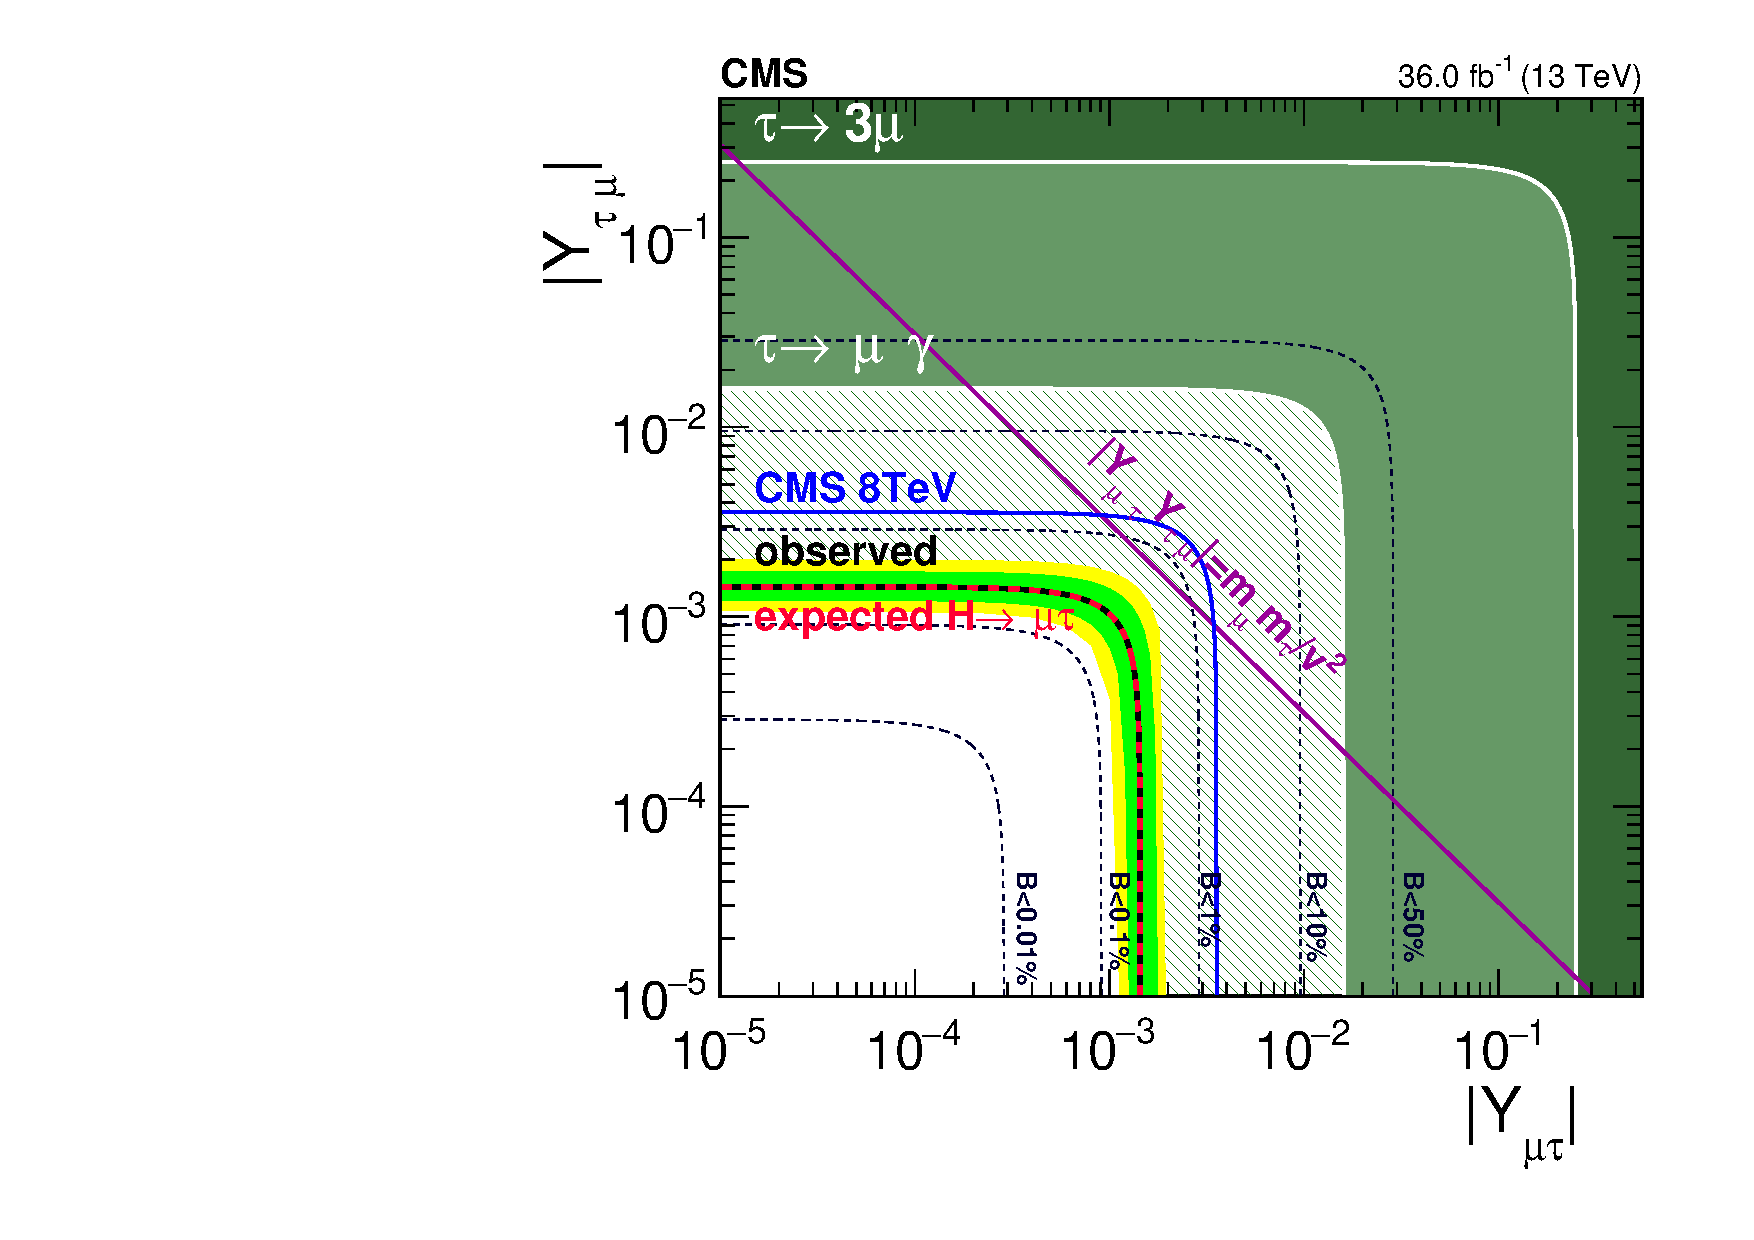
\includegraphics[width=0.45\textwidth]{plots/chapter2/Ymt.pdf}
  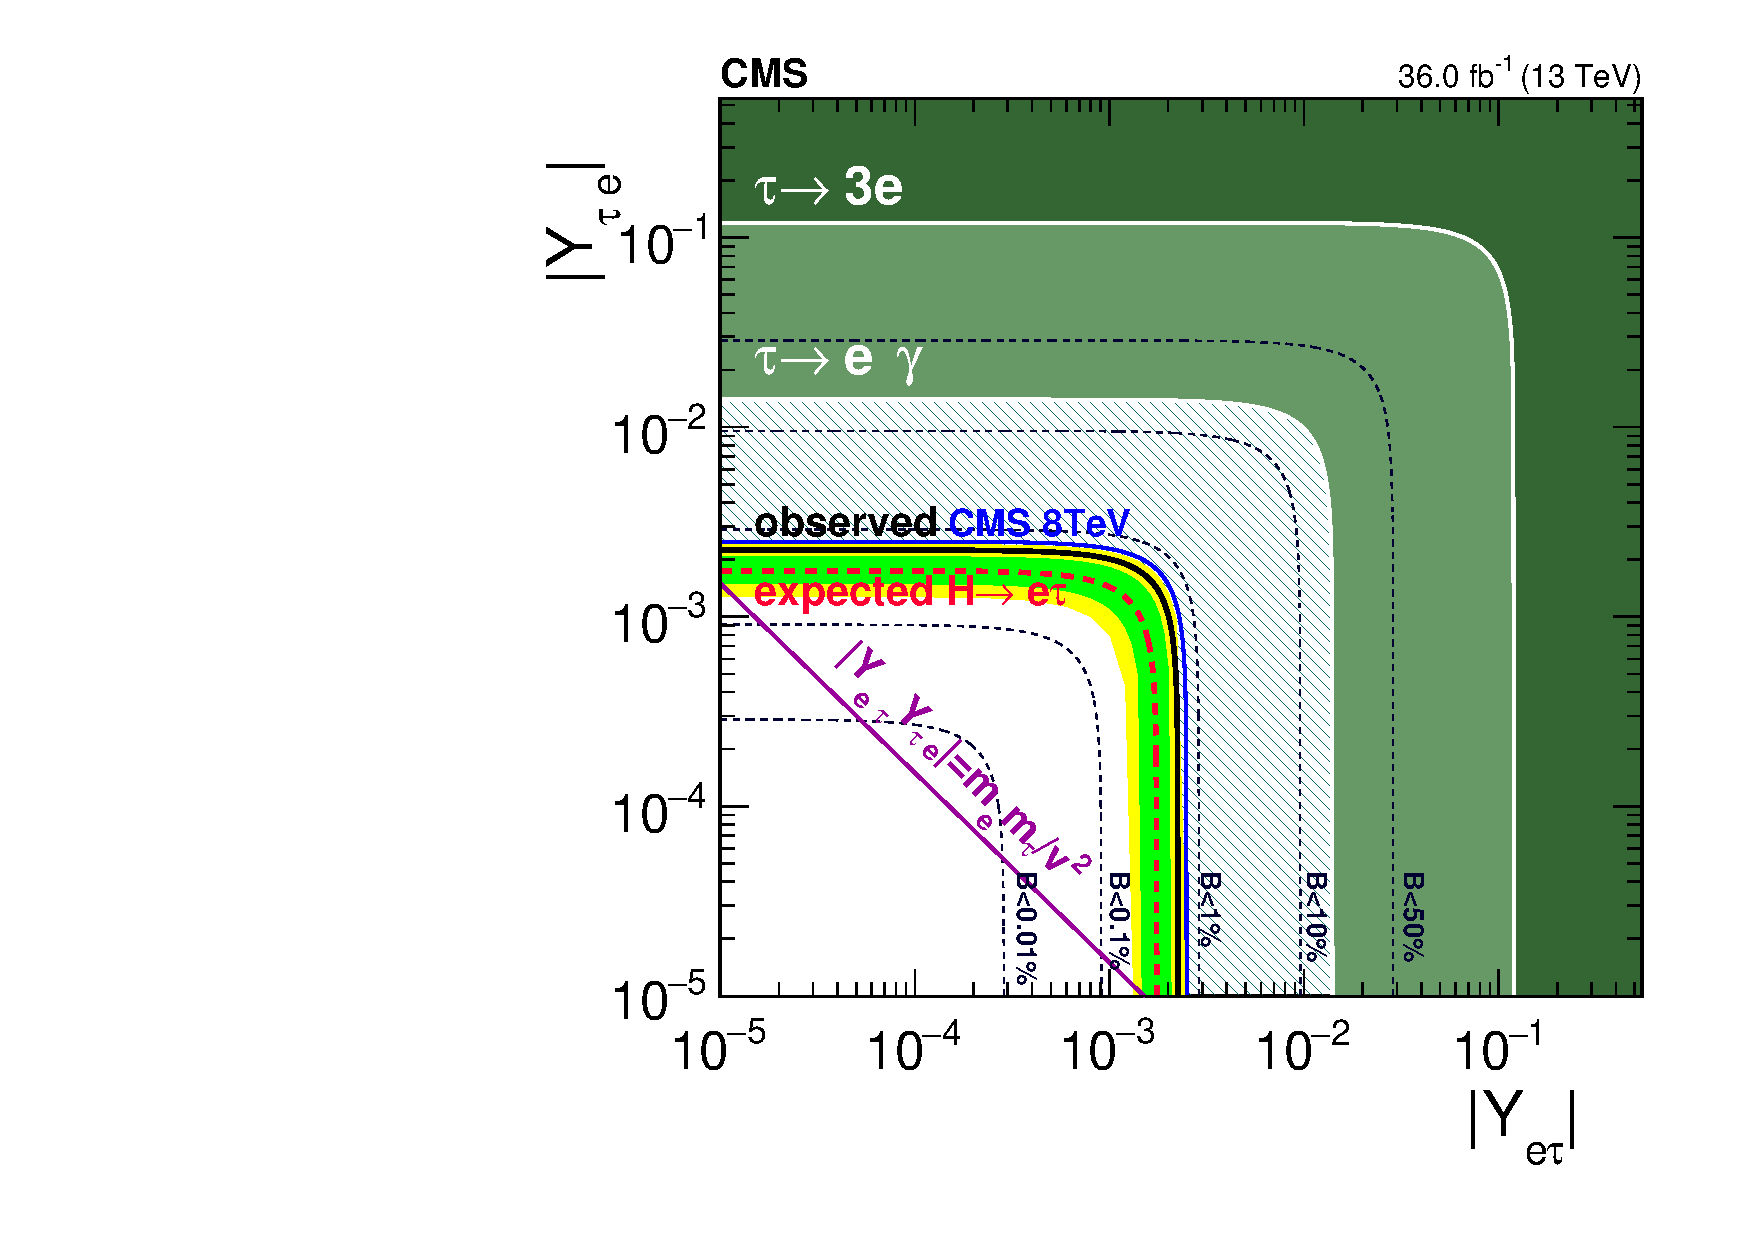
\includegraphics[width=0.45\textwidth]{plots/chapter2/Yet.pdf}
  \caption{Constraints on the LFV Yukawa couplings, $\Ymutau-\Ytaumu$ (left), and $\Yetau-\Ytaue$ (right) of the search performed by the CMS experiment.}
  \label{fig:yukawa}
\end{figure}

%
% Chapter 3
%

\chapter{LHC and the CMS detector}
\label{chap:exper_setup}

\section{Introduction}

The prime goals of the LHC and the Compact Muon Solenoid (CMS) \cite{Chatrchyan:2008aa} experiment are exploring the physics at the TeV scale and studying the mechanism of electroweak symmetry breaking, including studying the SM Higgs boson properties along with searches for new particles predicted by beyond the SM physics. The physics program's other main interests include studies of the SM top quark properties, electroweak physics, and physics of hadrons containing a charm or bottom quark. Heavy-ion collisions address the physics of strongly interacting matter and the quark-gluon plasma. Hadrons consist of quark and gluons; therefore, two colliding partons' initial energy is not known. In contrast, the collision's energy is known at lepton colliders, where each particle has the same energy. Thus, hadron colliders can explore a wide range of collision energies, while lepton colliders are well suited for precision measurements.

\section{The Large Hadron Collider}
\label{sec:LHC}

The LHC is a hadron accelerator located at CERN. The design was intended to collide proton beams with a beam energy of 7 TeV leading to a center-of-mass energy \sqs of 14 TeV and reach a luminosity of $10^{34} \lumi$. Lead (Pb) ions can be accelerated up to an energy of 2.8 TeV per nucleon and reach a luminosity of $10^{27} \lumi$. LHC is the most powerful tool for particle physics research that is currently available. The 26.7 km tunnel constructed between 1984 and 1989 for the Large Electron-Positron collider (LEP) \cite{Electron-Positron:1997351} was reused to install the LHC. There are eight arcs and eight straight sections lying 45-170 m below the surface. Unlike particle-antiparticle colliders that can use a single ring for both beams, the LHC uses two rings with counter-rotating beams. There is less synchrotron radiation owing to the heavier particles being collided at the LHC.

The accelerator complex acts as an injector of the protons and heavy ions. Protons are obtained from hydrogen gas after the electrons are stripped off, and they enter the Linear accelerator 2 (Linac2) \cite{accelerator:1997427}, where they are accelerated to 50 MeV. They are further accelerated in the Proton Synchrotron Booster (PSB) \cite{Synchrotron:1997372} to 1.4 GeV. They are then injected in the Proton Synchrotron (PS) \cite{Synchrotron:1997189}, where they are accelerated to 25 GeV. A bunch train is produced within the PS before extraction. The protons are then accelerated in the Super Proton Synchrotron (SPS) \cite{Synchrotron:1997188} to 450 GeV before injecting in the LHC.

The four interaction points are equipped with particle detectors: the CMS experiment, A Toroidal LHC ApparatuS (ATLAS) experiment \cite{Aad:2008zzm}, A Large Ion Collider Experiment (ALICE) \cite{Aamodt:2008zz}, and a Large Hadron Collider beauty (LHCb) \cite{Alves:2008zz} experiment. Two further smaller experiments, a Total, Elastic, and diffractive cross section Measurement (TOTEM) \cite{Anelli:2008zza} and the Large Hadron Collider forward (LHCf) \cite{Adriani:2008zz} experiment, are located near the CMS interaction point and near the ATLAS interaction point, respectively.

The ATLAS and CMS experiments have both multi-purpose detectors installed. The detectors were build to detect particles from proton-proton (p-p) or heavy-ion (Pb-Pb) collisions. One of the main tasks currently is to study the production and decay of the discovered Higgs boson \cite{Chatrchyan:2013lba}, disentangle its properties, and check if it is the SM Higgs boson or a Higgs boson of an extension of the SM. The other tasks involve high precision tests of QCD, electroweak interactions, and heavy flavor physics. Precision measurements of production, the couplings, and the spin of the top quark are also pursued. Several searches for supersymmetric particles and Dark Matter are also ongoing.

During the LHC Run II data-taking, a bunch spacing of 25 ns was used, and proton-proton collision data were collected at $\sqs = 13$ TeV in 2016, 2017, and 2018. The integrated luminosity delivered to CMS as a function of time is shown in Figure \ref{fig:lumi} for each proton-proton collision data-taking period. CMS does not record the whole delivered data, and only part of the recorded that is considered good is used for physics analysis.

\begin{table}[!hbpt]
  \centering
  \caption{Integrated luminosity considered for physics analysis at the CMS experiment during Run II}
  \begin{tabular}{|c|c|}
    \hline Year & Integrated luminosity \\
    \hline 2016 & $35.9 \fb$ \\
    \hline 2017 & $41.5 \fb$ \\
    \hline 2018 & $59.3 \fb$ \\
    \hline
  \end{tabular}
  \label{tab:luminosity}
\end{table}

\begin{figure}[htbp]
  \centering
  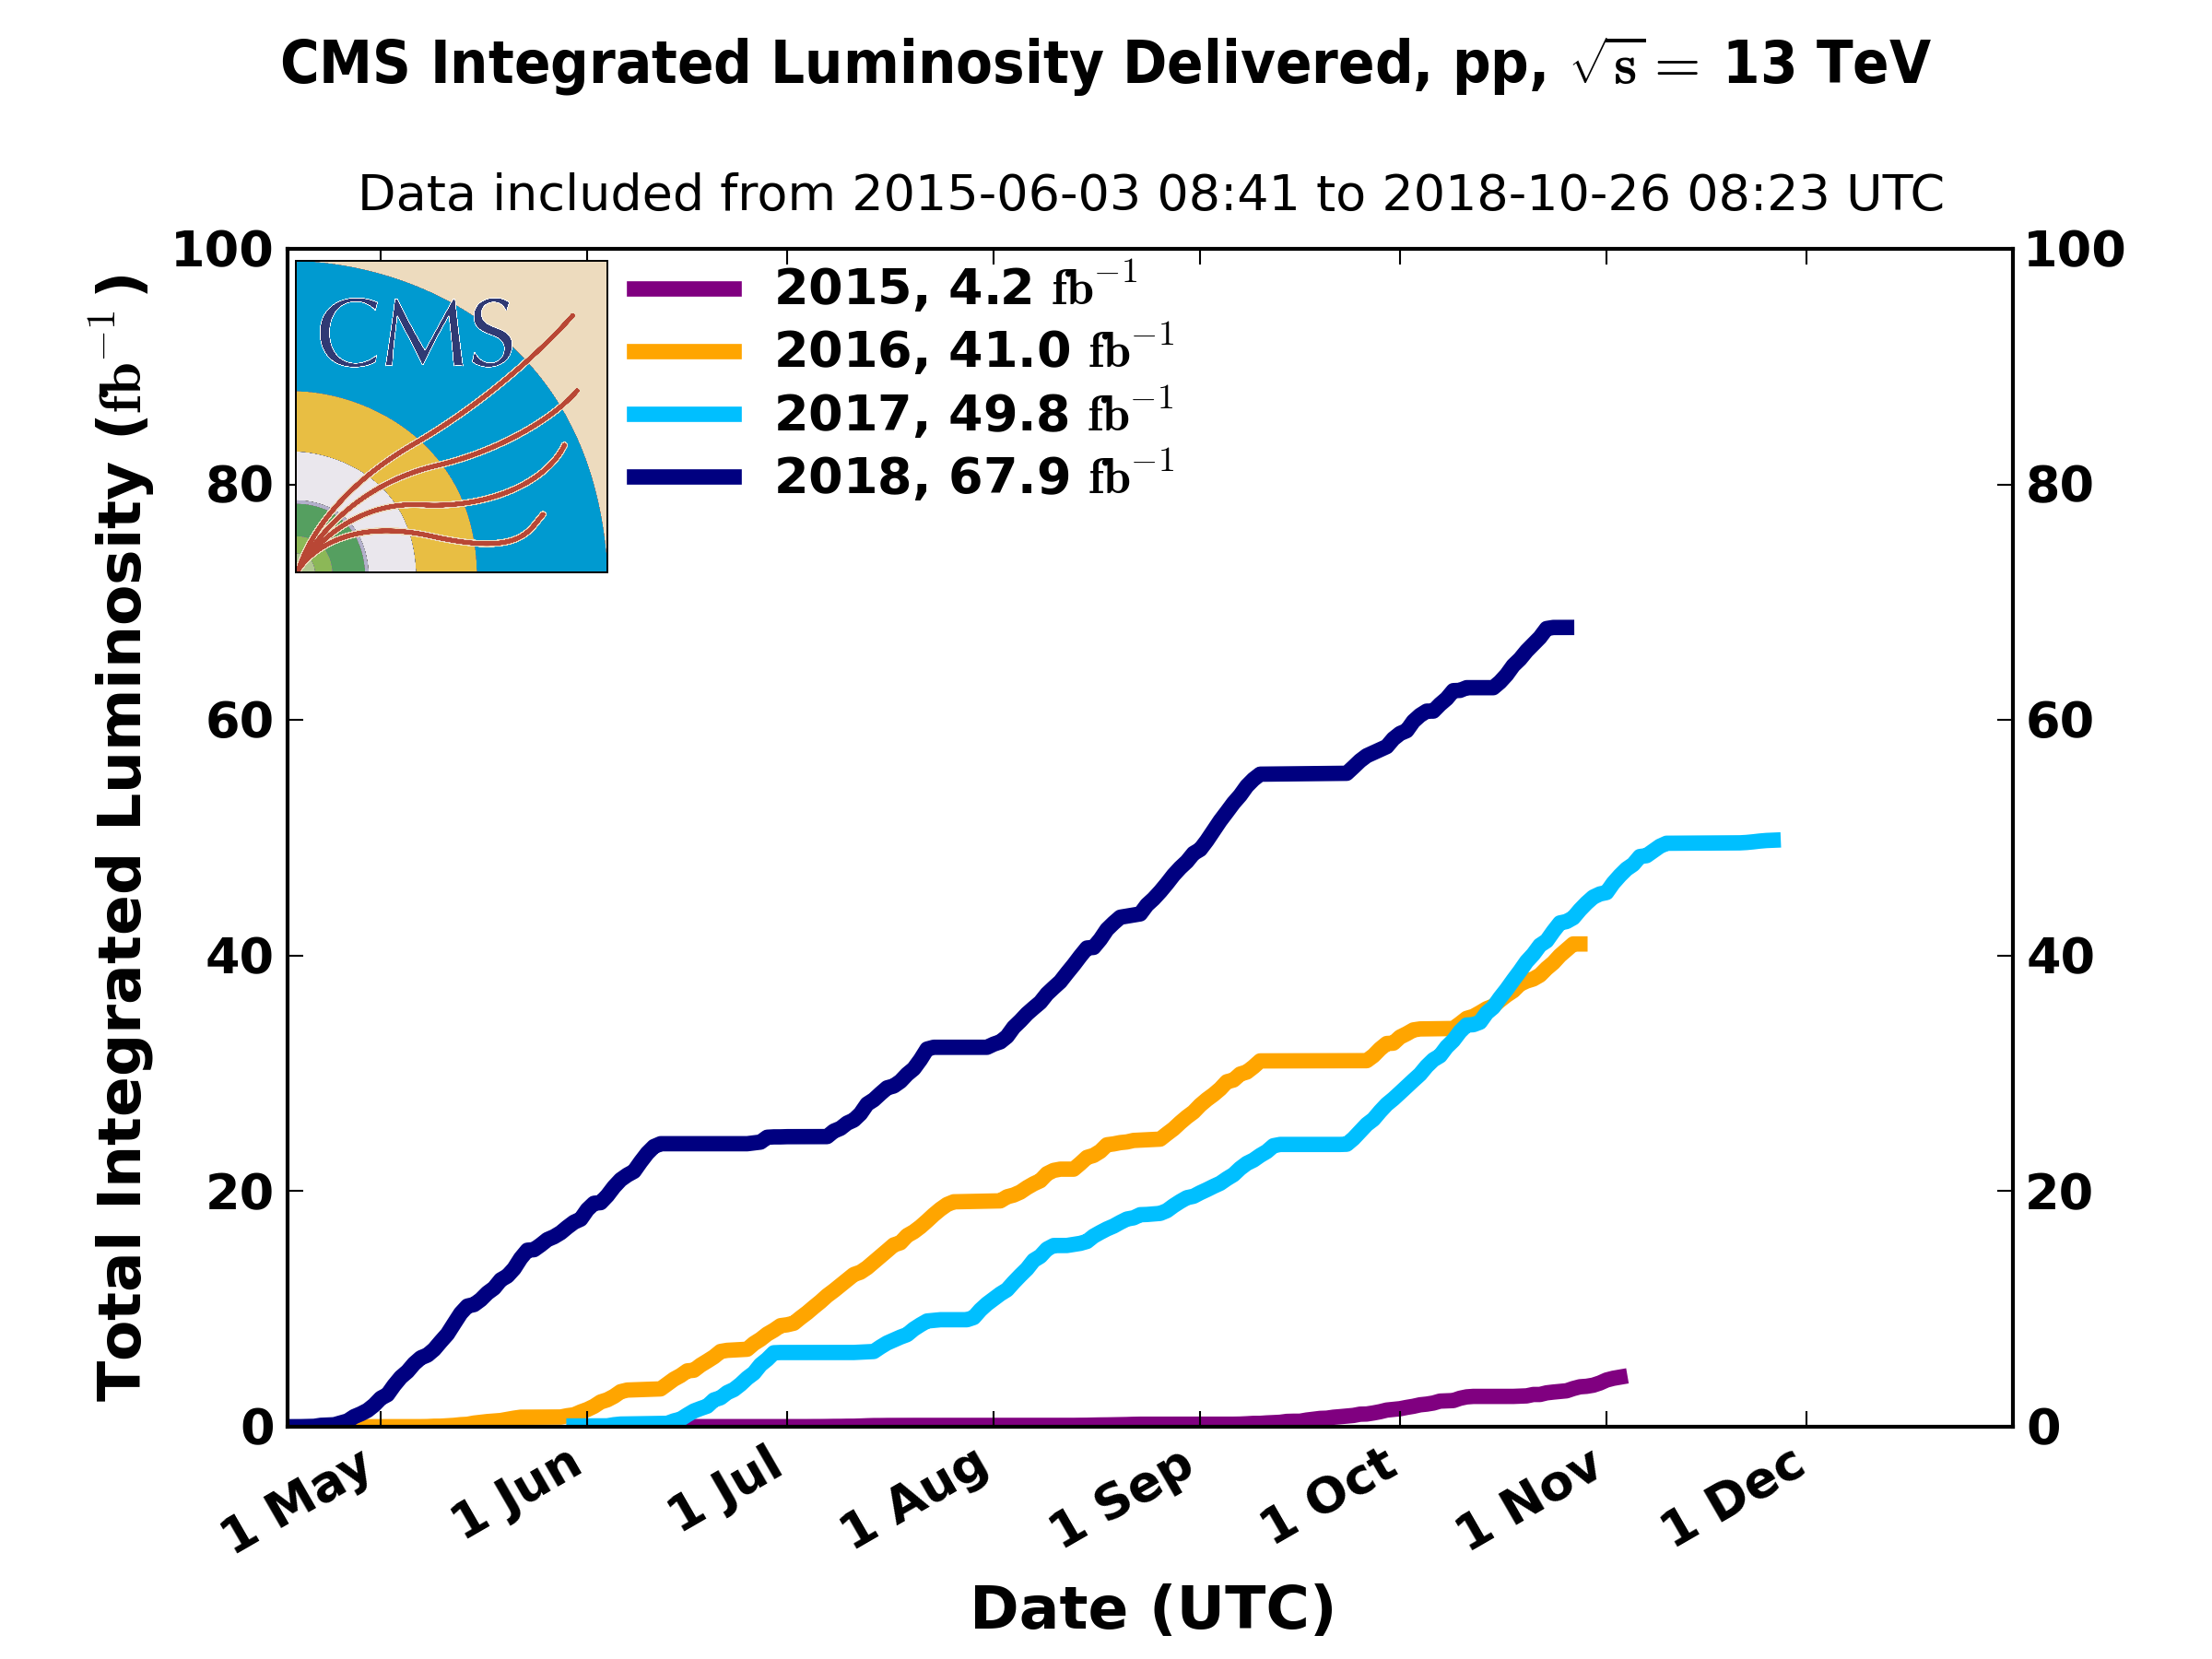
\includegraphics[width=0.8\textwidth]{plots/chapter3/int_lumi.png}
  \caption{Cumulative luminosity as a function of time delivered to CMS during stable beams for proton-proton collisions. The luminosity is shown for 2015 (purple), 2016 (orange), 2017 (light blue), and 2018 (dark blue). \cite{lumi}}
  \label{fig:lumi}
\end{figure}

\section{The Compact Muon Solenoid experiment}
The layout of the CMS detector is shown in Figure \ref{fig:cms}. As the name ``Compact Muon Solenoid'' indicates, a superconducting solenoid is the heart of CMS. Considerable bending power for the momentum measurement of charged particles within a compact design is achieved using a high magnetic field of 3.8 T. The internal part of the magnetic coil is large enough to accommodate the inner tracking system and the calorimetry. The inner tracking system is composed of a pixel detector close to the interaction region and a silicon strip tracker. The pixel detector can resolve individual vertices and distinguish between vertices from the primary interaction and secondary vertices from the decay of the primary interaction particles. Trajectories are precisely measured with the high granular silicon strip tracker, which can deal with high charged particle multiplicities.

\begin{figure}[htbp]
  \centering
  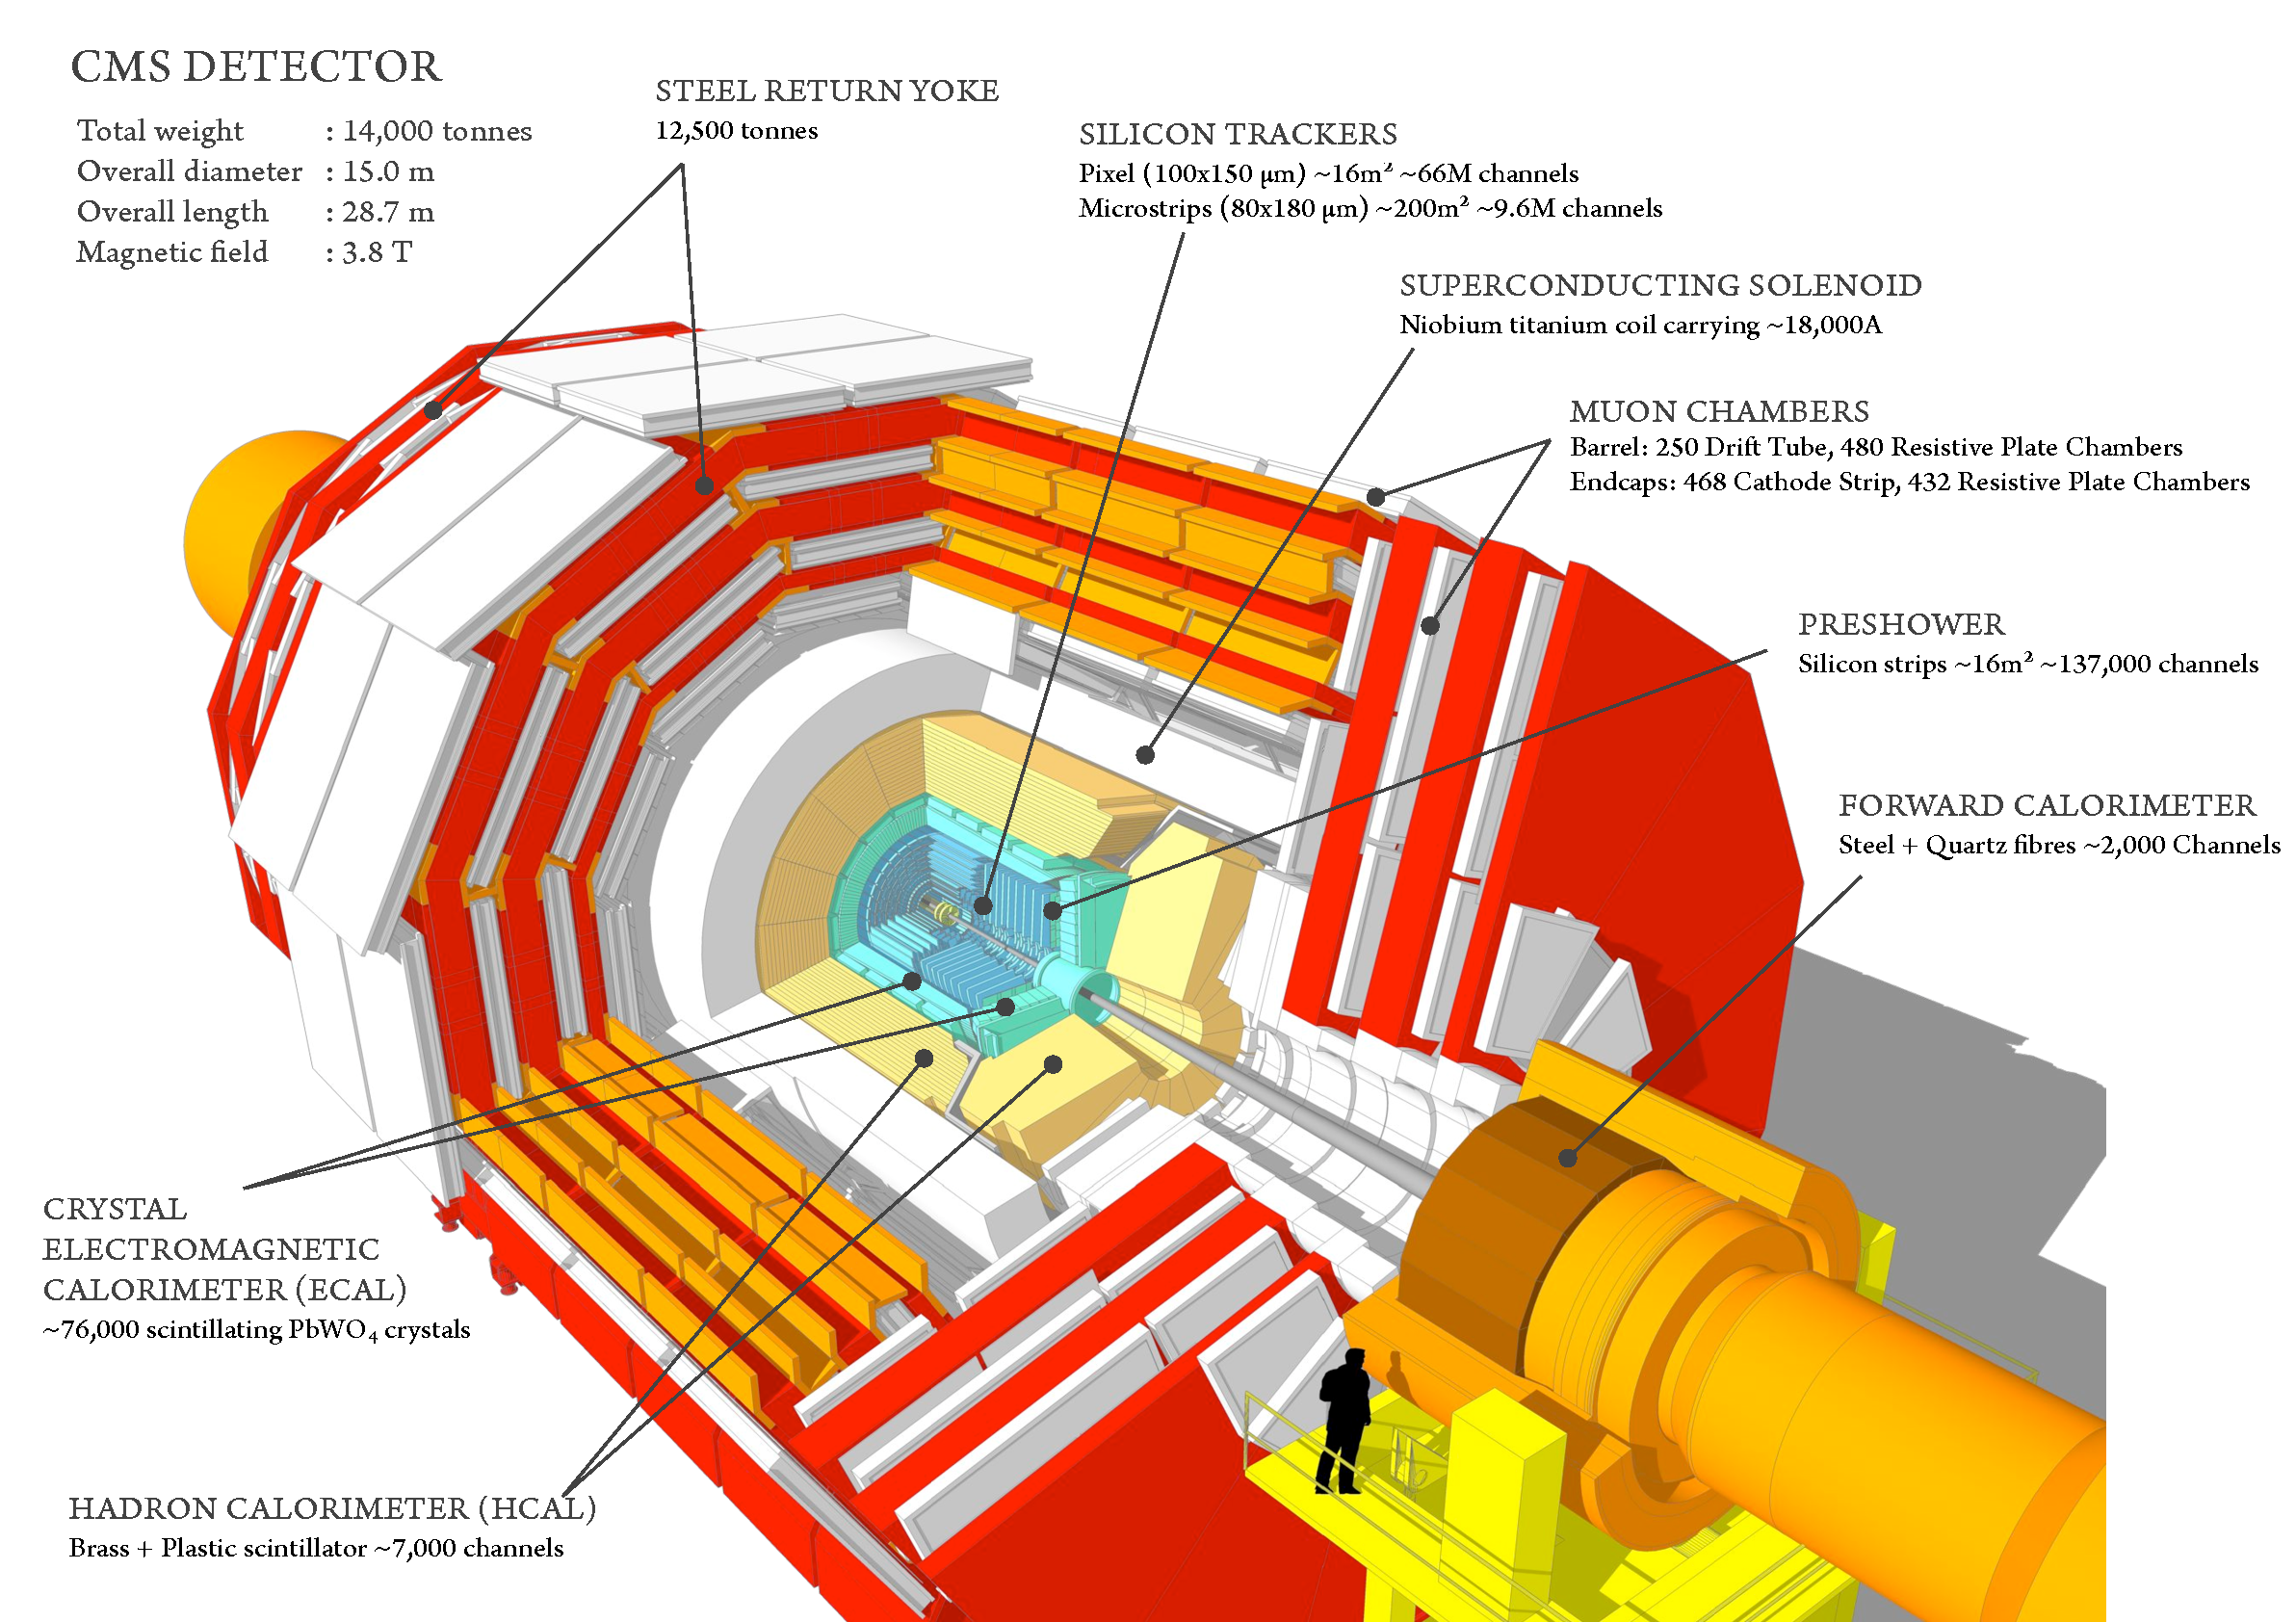
\includegraphics[width=0.9\textwidth]{plots/chapter3/cms_layered.png}
  \caption{Schematic view of the CMS detector.}
  \label{fig:cms}
\end{figure}

The energy of the particles is measured in calorimeters. Calorimeter material initiates electromagnetic (EM) or hadronic showers. For electromagnetic interactions, the characteristic interaction length is the radiation length $X_0$, while the characteristic interaction length for hadronic showers is the nuclear interaction length $\lambda_I$. The entire volume is sensitive in homogeneous calorimeters, while sampling calorimeters consist of metallic absorber sandwiched or threaded with an active material that generates the signal. CMS has an EM calorimeter (ECAL) made of lead tungstate $PbWO_{4}$ in front of a brass/scintillator sampling hadron calorimeter (HCAL). An additional layer of scintillators is outside the coil. The magnet is used as an absorber material. This iron/quartz-fiber calorimeter is referred to as the hadron outer (HO) detector. The muon detectors are sandwiched between the layers of the steel return yoke. Their main task is to trigger on muons and to identify the muons with good momentum resolution.

\subsection{The coordinate system of CMS}
CMS uses a right-handed Cartesian coordinate system with its origin at the detector's center, the nominal interaction point. The x-axis points towards the LHC center, while the y-axis points upward towards the surface and perpendicular to the LHC plane. Thus, the z-axis points along the anticlockwise beam-direction. Two angles are defined, where the azimuthal angle $\phi$ is measured from the x-axis in the x-y plane, and the polar angle $\theta$ is measured from the z-axis. Pseudorapidity is defined as

\begin{equation}
  \eta=-\ln \left[\tan \left(\frac{\theta}{2}\right)\right]
\end{equation}

and describes the angle of a particle relative to the beam axis, illustrated in Figure \ref{fig:coordinate}. Distances in $\phi$ and $\eta$ are denoted $\Delta\phi$ and $\Delta\eta$. These distance measures are used to define the spatial separation between physics objects by $\Delta R$ with

\begin{equation}
  \Delta \mathrm{R}=\sqrt{(\Delta \phi)^{2}+(\Delta \eta)^{2}}
\end{equation}

\begin{figure}[htbp]
  \centering
  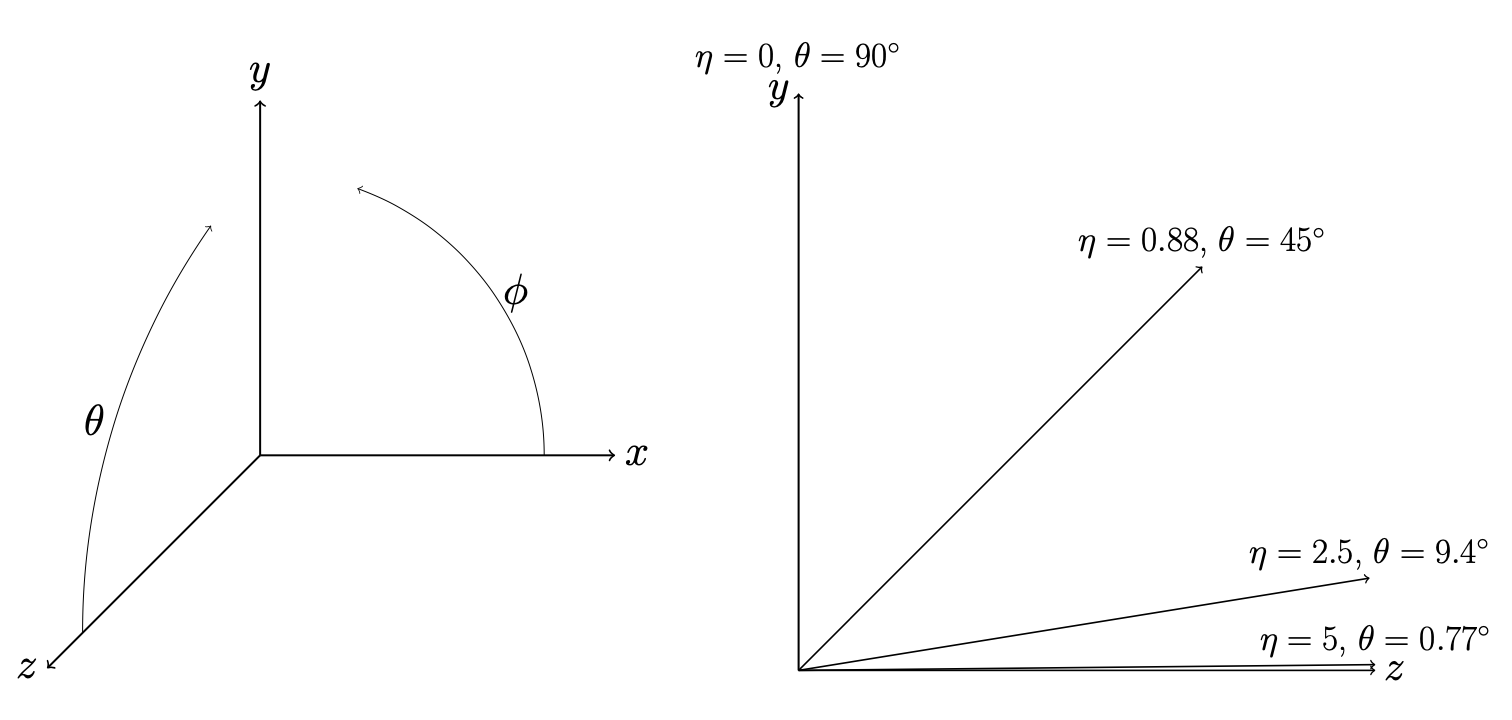
\includegraphics[width=0.9\textwidth]{plots/chapter3/coordinate.png}
  \caption{Coordinate system convention of CMS (left) and the relation between pseudorapidity $\eta$ and polar angle $\theta$ (right)}
  \label{fig:coordinate}
\end{figure}

\subsection{Kinematic quantities}
At LHC, the protons carry half of the collision energy \sqs. The hard interactions do not take place between the colliding protons but between two of their partons. Each parton carries a fraction of $x_i$ of the proton momentum. As the parton mass can be neglected with respect to the momentum $\vec{p}$, the parton energy is given by its momentum. In the laboratory frame, the four-momenta of the partons are

\begin{equation}
  \mathrm{p}_{1}=x_{1} \cdot \frac{\sqs}{2}(1,0,0,1) \\
  \mathrm{p}_{2}=x_{2} \cdot \frac{\sqs}{2}(1,0,0,-1)
\end{equation}

Then, the invariant mass M of the hard collision is given by

\begin{equation}
  \hat{s} \equiv \mathrm{M}^{2}=\left(\mathrm{p}_{1}+\mathrm{p}_{2}\right)^{2}=\frac{s}{4} \cdot\left[\left(x_{1}+x_{2}\right)^{2}-\left(x_{1}-x_{2}\right)^{2}\right]=x_{1} x_{2} s
\end{equation}

where $\sqrt{\hat{s}}$ denotes the center-of-mass energy of the parton-parton collision. The hard collision products have a total momentum, zero for the x- and y-components but in general non-zero for the z-component. Thus, the hard-collision products' momentum and energy are measured transverse to the beam direction in the x-y plane. \pt and \ET denote the transverse momentum and transverse energy respectively, with $\ET = \text{E} \cdot \text{sin} \theta$. Only weakly interacting particles, such as neutrinos, do not produce a signal in the CMS detector and lead to an imbalance in the observed total transverse momentum in the event, missing transverse energy, denoted as \met.

\subsection{Detector requirements}
Final states that contain isolated leptons and photons leave clean signatures in the CMS detector. A good muon identification and momentum resolution are needed over a wide range of momenta. The muon charge has to be determined unambiguously. Furthermore, a good momentum resolution and reconstruction efficiency of charged particles are crucial for reconstructing electrons and charged hadrons. Charged-particle momenta are measured using the curvature of their trajectory. Considerable bending power is needed to measure precisely the momentum of particles with large momentum. Additionally, a good electromagnetic energy resolution is needed with wide geometrical coverage. The direction of the photons and correct localization of the primary interaction should be measurable.

Quarks hadronize, and the hadrons can be detected with the CMS detector. Good identification of hadronically decaying taus is needed for the Higgs boson physics. The triggering and identification efficiency of hadronically decaying taus can be improved by a good measurement of the impact parameter of charged-particle tracks and good position measurement of the secondary vertices. This requires pixel detectors close to the interaction region. Hadronic calorimeters with a large hermetic coverage ($|\eta| < 5$) and with a fine lateral segmentation $(\Delta \eta \times \Delta \phi<0.1 \times 0.1)$ are required for a good energy measurement of hadrons and estimation of \met.

The collisions are happening at a rate of $40 \mathrm{MHz}$ and not all of these events can be stored; therefore, only interesting events have to be selected. The online event selection process, trigger, must reduce the rate to no more than a few hundred events per second. The short time between two bunch crossings, 25 ns, has a major implication on the readout and trigger system design. Multiple proton-proton interactions (pileup) happen in one bunch crossing. The interactions' products overlap and can be wrongly linked. Long response times of detector elements and their electronic signal longer than 25 ns increase this effect. High granularity detectors with good time resolution result in a low occupancy. This requires many detector channels and, therefore, a good synchronization of the electronic detector channels. The large flux of the particles and resulting high radiation levels require radiation-hard detectors and front-end electronics.

\subsection{Magnet}

The curvature of the particle trajectory in a magnetic field determines the momenta and sign of charged particles. The most important aspect of muon measurement is the choice of magnetic field configuration. A good momentum resolution of $\Delta \mathrm{p} / \mathrm{p} \approx 10 \%$ is required for muons with a momentum of 1 TeV. CMS uses a large superconducting solenoid with a magnetic field of 3.8 T. The solenoid is 13 m long and has an inner diameter of 5.9 m. The superconductor material is Niobium titanium \cite{BUL-NA-2003-150}. A high-purity aluminum-stabilized conductor with a four-layer winding is used, which has to withstand outward pressure. The conductor is composed of five coils, and its superconducting wire is cooled using an indirect cooling by thermosyphon.

\subsection{Inner Tracking system}

The inner tracking system \cite{Khachatryan:2010pw} measures the trajectories of particles up to $|\eta| < 2.5$. The particle flux is the highest close to the interaction region. The silicon pixel detector is placed close to the interaction region. This allows for the reconstruction of vertices from heavy flavor hadrons with a b or c quark. Each pixel has a size of $\approx 100 \times 150 \mum^{2}$. The spatial resolution of the radius and azimuthal angle $r-\phi$ measurement is about 10 $\mu m$, and 20 $\mu m$ for the z-coordinate measurement. In the intermediate region ($20 < r < 55$ \cm) and outermost region ($r > 55$ \cm) silicon microstrips are used with a size of $10 \cm \times 80 \mum$ (minimum cell size) and a size of $25 \cm \times 180 \mum$ (maximum cell size), which provide the required granularity. The barrel's tracking volume has a cylinder shape with a length of 5.8 m and a diameter of 2.6 m. The pixel detector consists of three layers at radii of 4, 7, and 11 \cm in the barrel.

Additionally, there are ten layers of silicon microstrip detectors. The strip tracker is divided into a Tracker Inner Barrel (TIB) made out of four layers and a Tracker Outer Barrel (TOB) made out of six layers. Each part has two layers which provide a single-point measurement in the $r - \phi$ and $r - z$ coordinates. In the TIB, the single-point resolution is $23 - 34 \mum$ in the r-direction and $23 \mum$ in z, while it is $35 - 52 \mum$ in the $r-\phi$ direction and $52 \mum$ in $z$ for the TOB. In the two end caps, there are just two-pixel layers and nine microstrip layers. The strip tracker's endcaps are divided into the Tracker End Cap made of 9 disks and the Tracker Inner Disks (TID), which are made of three small disks, which fill the gap between the TIB and the TEC.

\subsection{Electromagnetic Calorimeter}

The electromagnetic calorimeter (ECAL) measures the energy of electrons and photons. A hermetic, homogeneous crystal (ECAL) with a coverage of $|\eta| < 3$ is used, which has an excellent energy resolution and high granularity; therefore, it also has excellent separation of close clusters \cite{CMS:2010bta, Khachatryan:2015hwa}. It is used to identify photons, which leave no signal in the inner tracking detector. Lead tungstate ($PbWO_4$) crystals are used, which have a short radiation length of $X_0 = 0.89$ \cm, are radiation hard, and emit blue-green scintillation light with a maximum at 420 nm. The scintillation decay time is short and in the same order as the LHC bunch crossing time. About 80\% of the light is emitted within 25 ns. However, the light output depends on the temperature; therefore, a cooling system is needed to preserve the energy resolution. Furthermore, a low light yield requires photodetectors with intrinsic gain that can also operate in a high magnetic field. The crystals allow a compact calorimeter inside the solenoid that is fast, has a fine granularity, and is radiation-resistant. Figure \ref{fig:ecal} illustrates the layout of the CMS ECAL. The calorimeter is divided into a barrel ECAL (EB) which covers the region $0 < |\eta| < 1.479$ and two ECAL endcaps (EE) which cover the region $1.479 < |\eta| < 3.0$. Preshower detectors (ES) are installed in front of each endcap and cover the region $1.653 < |\eta| < 2.6$. In the EB, silicon avalanche photodiodes (APDs) are installed to detect the scintillation light. They also respond to temperature changes; therefore, they require a stable temperature.

\begin{figure}[htbp]
  \centering
  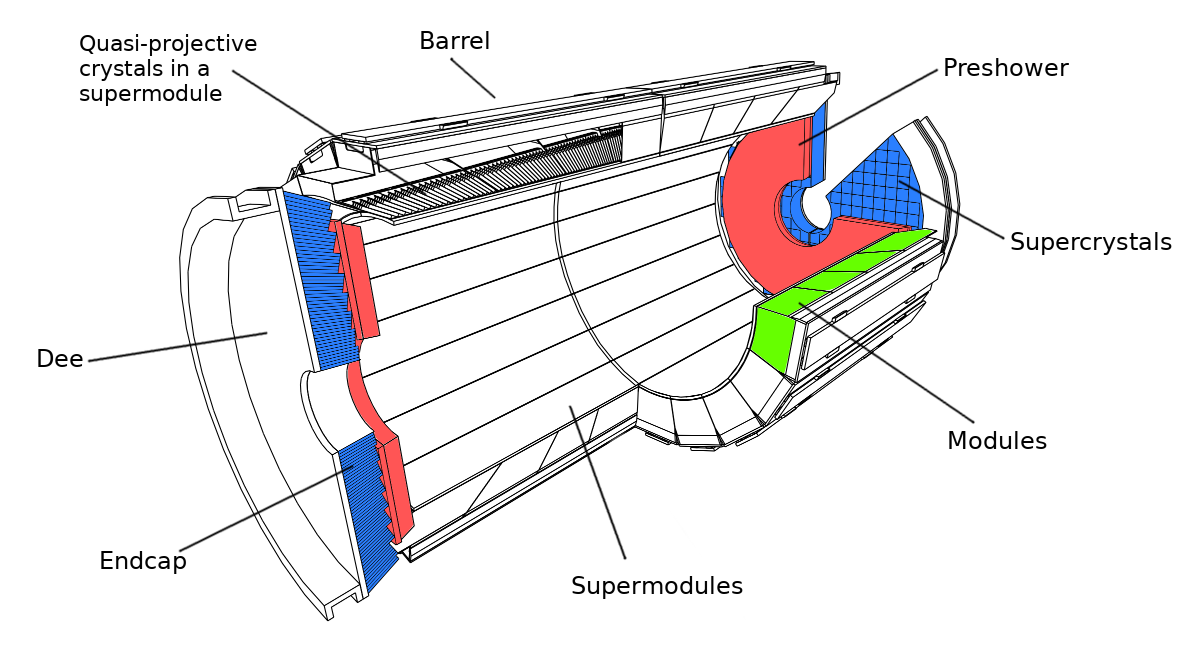
\includegraphics[width=0.9\textwidth]{plots/chapter3/ecal.png}
  \caption{Schematic view of the electromagnetic calorimeter.}
  \label{fig:ecal}
\end{figure}

The barrel section is structured in 36 identical supermodules, 18 in each half barrel, with the crystals being arranged in a grid and covering $\Delta \eta \times \Delta \phi=0.0174 \times 0.0174$. Vacuum phototriodes (VPTs) are installed in both EE for detecting the scintillation light. The crystals are arranged in units of $5 \times 5$ crystals termed super crystals (SC). Both the crystals and the SCs, are arranged in a rectangular x-y grid. Neutral pions dominantly decay to two photons. Two closely separated photons can mimic high-energy photons; therefore, a preshower system is installed in front of each EE to identify and reject $\pi^0$ mesons. It also improves the position determination of electrons and photons as it has a higher granularity than the EE. The preshower detector is a sampling calorimeter consisting of two layers of a lead absorber, which initiate the electromagnetic showers from incoming electrons or photons. Each lead radiator is followed by silicon strip sensors measuring the energy deposits and the transverse shower profiles. The strips in both planes of silicon sensors are orthogonal oriented and are placed after a radiation length of 1 $X_0$ and 2 $X_0$ of the lead absorber.

\subsection{Hadron Calorimeter}
The energy of hadrons is measured in the hadron calorimeter (HCAL). Most of the HCAL calorimetry is located inside the magnetic coil surrounding the ECAL system. An important requirement on the HCAL design is to minimize the non-Gaussian tails in the energy resolution and to provide a good hermeticity for the determination of \met. It is designed to maximize the interaction length of the material within the magnet coil. On the other hand, the amount of space devoted to the active medium is minimized. The HCAL is a sampling calorimeter which is divided into a hadron barrel (HB) detector, covering the region $|\eta| < 1.4$ and two hadron endcap (HE) detectors, covering $1.3 < |\eta| < 3.0$. Brass is used as an absorber material. Brass has a reasonably short interaction length, is easy to machine, and it is non-magnetic. A tile/fiber technology made of plastic scintillator tiles is used as an active medium. For the innermost and the outermost layer, stainless steel is used for structural strength. The 3.7-mm-thick scintillator plates are sandwiched between the absorber plates. Wavelength-shifting (WLS) fibers, embedded in the scintillator tiles, convert the scintillation light. Then, it is channeled to photodetectors via optical fibers. Multi-channel hybrid photodiodes (HPDs) detect the light. They can operate in high axial magnetic fields. The HB is read out as a single longitudinal sampling with a segmentation $\Delta \eta \times \Delta \phi=0.087 \times 0.087 \approx 5^{\circ} \times 5^{\circ}$, which are termed tower. In the HE, the $\phi$ segmentation is $5^{\circ} - 10^{\circ}$ and the $\eta$ segmentation is $0.087 - 0.35$ depending on $\eta$.

Additional layers of scintillators are installed outside the coil within the return yoke using the iron as an absorber—the sample energy from hadron showers, which leak through the rear of the calorimeters. The central shower containment and the \met resolution of the calorimeter are thus improved. This sampling calorimeter is referred to as Hadron Outer (HO) detector. It is located along with the barrel muon system; therefore, its segmentation closely follows the barrel muon system. It is divided into five sections along with $\eta$ termed rings. The HO follows the HCAL barrel geometry in $\eta$ and $\phi$ and covers the region $|\eta| < 1.26$. Two further detectors, which cover the region $2.9 < |\eta| < 5.0$, are not shown. They are specialized in measuring energetic forward hadronic showers and ensuring full geometric coverage for the transverse energy measurement. The Hadron Forward (HF) sampling calorimeters use steel as absorber material and quartz fibers as the active medium, which run parallel to the beam. Shower particles in the quartz emit Cherenkov light fibers. This light is channeled by the fibers to photomultipliers. There are two types of quartz fibers, long ones (1.65 m) and short ones (1.43 m). Neutral components of the hadron showers are preferentially sampled in the HF, leading to narrower and shorter hadronic showers. This is ideally suited for the forward region. The towers in HF have a segmentation of $0.1 - 0.3$ and a $\phi$ segmentation of $10^{\circ}$, except in high $\eta$-towers, where $\phi$ segmentation is $20^{\circ}$.

\subsection{Muon System}

The Muon system is installed in the magnet return yokes of CMS. Its main tasks are identifying muons, improving the \pt measurement, and charge-sign determination of high-\pt muons. Additionally, it is used to trigger muons. It is divided into a barrel detector (MB) covering $|\eta| < 1.2$ and two endcap detectors (ME), covering the region $0.9 < |\eta| < 2.4$, defining three regions: the barrel region ($|\eta| < 0.9$), the overlap region ($0.9 < |\eta| < 1.2$), and the endcap region ($1.2 < |\eta| < 2.4$). Three different types of gaseous detectors are used in different radiation environments. Drift tube (DT) chambers are used in the barrel region, where the muon rate, the neutron-induced background rate, and the residual magnetic field are low. In the two endcaps, the muon rate, neutron-induced background, and the magnetic field are high; therefore, cathode strip chambers (CSC) are used in this region. Resistive plate chambers (RPC) are used in both subdetectors covering the region $|\eta| < 1.6$. They are operated in avalanche mode to ensure good operation at high rates. The RPCs have double gaps with a width of 2 mm filled with gas. They have a fast response with a good time resolution but a coarser position resolution than the DTs and CSCs; therefore, they are used to identify the correct bunch crossing.

Figure \ref{fig:muon} gives an overview of the layout of the muon system. The MB is divided into four stations arranged in cylinders interleaved with the iron yoke. Additionally, it is divided into five wheels along the beam direction following the five wheels of the return yokes. Each chamber consists of 12 layers divided into 3 Super Layers (SL), made out of four DTs layers. Two SL measure the $r-\phi$ coordinate, while a third SL sandwiched in between them measures the $z$ coordinate. In the last muon station, there are only two SL to measure the $r-\phi$ coordinate. Each DT chamber has one or two associated RPCs. The single point resolution of the DTs is $\approx 200 \mum$. In each endcap, the CSCs and RPCs are arranged in four disks. They are divided into three or two concentric rings in the innermost station and other stations. Each CSC measures up to six space coordinates $(r, \phi, z)$ and the provided spatial resolution is $\approx 200 \mum$, except for the innermost ring in the first disk, where it is $\approx 100 \mum$. The angular resolution in $\phi$ is $\sim 10 mrad$. Two independent and complementary information sources come from the DTs or CSCs and the RPCs, which feed the trigger system.

\begin{figure}[htbp]
  \centering
  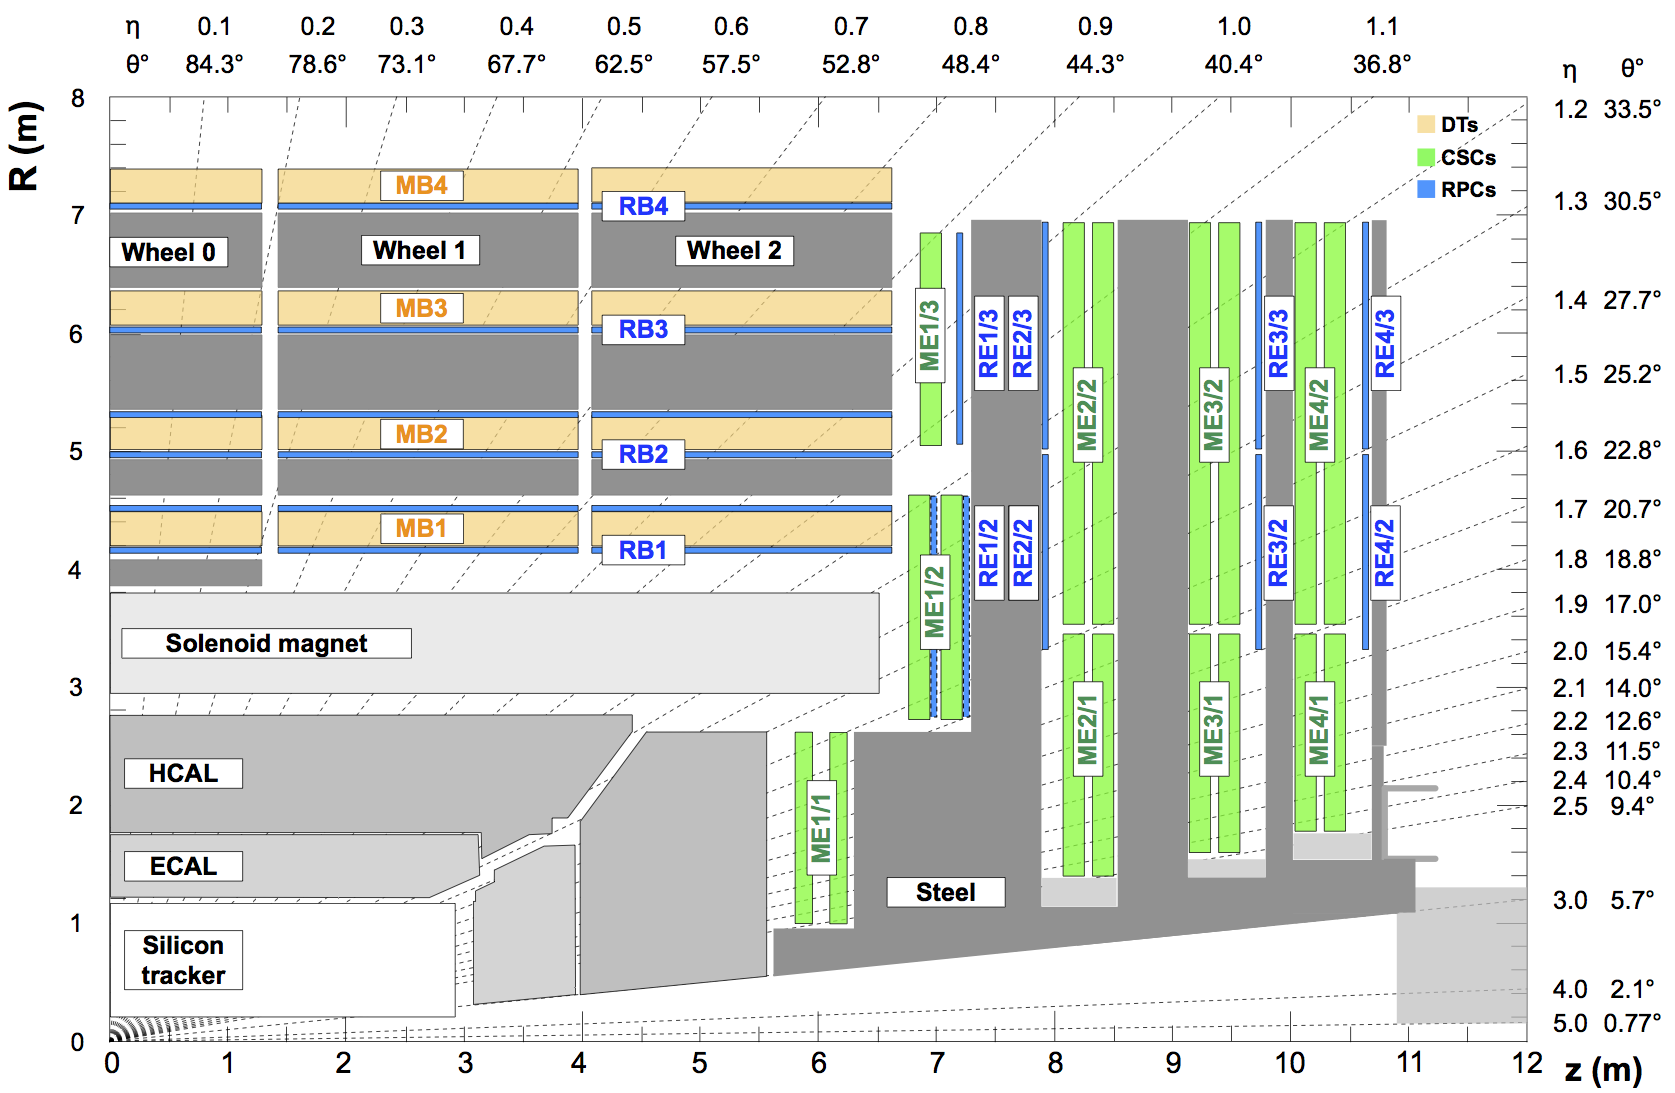
\includegraphics[width=0.9\textwidth]{plots/chapter3/muon.png}
  \caption{Schematic view of the muon detectors.}
  \label{fig:muon}
\end{figure}

\subsection{Trigger and data acquisition system}

The online event selection process, trigger, reduces the rate to about $1 \mathrm{KHz}$. The CMS experiment's trigger and data acquisition system is divided into four parts, summarised in Figure ?. First, the detector electronics detect signals and pass them to the Level-1 trigger processors. The Level-1 trigger logic is located in a service cavern and selects events of interest. Due to the size of the CMS detector and underground caverns, the transit and time needed for a decision is about 3.2 $\mu s$. However, the time needed for Level-1 trigger calculations is only 1 $\mu s$. At this time, the data is held in pipelined memory buffers.

Custom hardware processors form the Level-1 decision to keep or discard data using the calorimetry, muon systems, and correlation information. Trigger primitive objects, such as electrons or muons above a set \ET or \pt thresholds are used for the decision taking. Reduced granularity and resolution data are used to form the trigger objects. Sums of \ET and \met are also employed. Only about one out of 1000 interactions are retained. If the data of interaction is kept, the data is transferred after a fixed time interval of about $3.2 \mu s$ to the front-end readout buffers. The data is further processed and compressed, and placed in dual-port memories. A processor farm is responsible for filtering the events. Each processor runs the same High-Level Trigger (HLT) code, reducing the output rate from a few kHz to a few hundred Hz for mass storage. Using a processor farm for event filtering allows for computer technology evolution and maximizes the flexibility in selecting data and algorithms. Whenever possible, only necessary objects are reconstructed, and only needed information of some subdetectors are used. The idea of partial reconstruction and many virtual trigger levels is the basis for the HLT. First, calorimeter and muon information is used, followed by the use of pixel tracker data. Finally, the full event information is used, including full tracking. The HLT system uses identification and isolation criteria as well as minimal energy or transverse momentum thresholds.

\subsection{Luminosity measurement}

Luminosity L is defined as the ratio of the event rate $\dot{\mathrm{N}}$ to the cross-section $\sigma$ of a given process, and it is the effective area quantifying the likelihood of a scattering event.

\begin{equation}
  \mathcal{L}=\frac{\dot{\mathrm{N}}}{\sigma}
\end{equation}

The cross-section is measured in units of area, thus the luminosity is given in units of events per time per area, $(b.s)^{-1} = 10^{24} \lumi$. Then, the integrated luminosity L is the integral over the instantaneous luminosity:

\begin{equation}
  \mathrm{L}=\int \mathcal{L}(t) d t
\end{equation}

For a given process, the number of expected events which are produced is given by the product of the integrated luminosity and the production cross-section $\sigma_{exp}$:

\begin{equation}
  \mathrm{N_{exp}}=\mathrm{L} \cdot \sigma_{exp}
\end{equation}

Thus, the integrated luminosity has to be known to estimate the number of events for a given process or measure the production cross-section. Luminosity measurements are used to monitor the LHC performance in real-time, and they provide an overall normalization for physics analyses \cite{Bayatian:2006nff}. A reference process can be used to estimate the cross-section of a given process:

\begin{equation}
  \sigma_{\exp }=\frac{N_{\exp }}{N_{\text {ref }}} \cdot \sigma_{\text {ref }}
\end{equation}

where $N_{ref}$ and $\sigma_{ref}$ are the number of reference events and the reference process's cross-section. Furthermore, the same integrated luminosity has to be used for both processes. Colliders used nowadays employ bunched beams \cite{Tanabashi:2018oca}. If two bunches with $n_1$ and $n_2$ particles, respectively, collide head-on with frequency f, the instantaneous luminosity is given by:

\begin{equation}
\mathcal{L}=f \cdot \frac{n_{1} n_{2}}{\sqrt{\epsilon_{x} \beta_{x}^{*} \epsilon_{y} \beta_{y}^{*}}}
\end{equation}

where ${x,y}$ are the coordinates transverse to the beam, $\beta^*_{x,y}$ are the amplitude functions at the interaction point, where the beam optics produces a narrow focus. Emittance $\epsilon$ is a measure of the beam width defined as $\epsilon_{x} \equiv \frac{\sigma_{x}^{2}}{\beta_{x}}$, with $\sigma_{x}$ and $\sigma_{y}$ being the root mean square (RMS) of the transverse beam sizes in the horizontal or vertical direction, respectively. A high luminosity can be achieved with a high population of bunches of low emittance colliding at high frequency at locations where the beam optics provide low values of the amplitude functions. As the instantaneous luminosity depends on the beam parameters, it has to be measured when the beam parameter change. A reference process's event rate can estimate the instantaneous luminosity if the cross-section is known. The visible cross-section $\sigma_{vis}$ is given by:

\begin{equation}
  \sigma_{\mathrm{vis}}=\sigma(\mathrm{E}) \cdot \mathrm{A}(t, \mu, \ldots)
\end{equation}

where the cross-sections depend on the collision energy E and the detector acceptance A depends on time t, the mean number of interactions per bunch crossing $\mu$, and other parameters. Luminometers are independent detectors or parts of the detector for measuring the instantaneous luminosity. Once the calibration constant $\sigma_{vis}$ has been determined for a luminometer, the luminosity can be estimated using

\begin{equation}
  \mathcal{L}=\frac{\dot{\mathrm{N}}}{\sigma_{\mathrm{vis}}}
\end{equation}

where $\dot{\mathrm{N}}$ is the event rate for this luminometer. Ideally, the luminometer's visible cross-section should not be time-dependent and should not depend on experimental conditions. The visible cross-section has to be determined again when the beam parameters change. The same detector configuration has to be used during data-taking as during calibration. In summary, there are two important parts of the luminosity measurement. First, the luminometer, which measures the event rate. Secondly, the calibration of the luminometer. In the following, both parts of the luminosity measurement are introduced.

Luminometer: CMS uses five detectors to monitor and measure the luminosity based on rate measurements \cite{CMS:2019jhq, CMS:2018elu, CMS:2017sdi}. The CMS silicon pixel detector, the DTs in the muon system's barrel, the forward hadronic calorimeter, the Fast Beam Conditions Monitor (BCM1f), and the Pixel Luminosity Telescope (PLT) are used as luminometers. The luminometer of the pixel detector and the DTs use the standard CMS trigger and data acquisition system, while the PLT, BCM1f, and HF have an independent, fast readout system. However, the silicon pixel detector and the DT have very low occupancy and very good stability over time. In LHC Run I, only the silicon pixel detector and the HF were used as luminometers \cite{CMS:2013gfa}.

The HF has a high rate of acquisition, and it is most sensitive to the electromagnetic component of the hadronic showers. Two methods have been studied to estimate the luminosity. The first one, referred to as zero-counting, counts the hits above the single physical towers' threshold and averages each tower's result. The second method exploits the linear relationship between the total transverse energy deposit in the HF and the number of interactions and the luminosity. Both methods require that the mean value of interactions $\mu$ is proportional to the luminosity. The Pixel Cluster Counting (PCC) method employs a large number of pixels in the CMS detector. A given pixel has an exceedingly small probability of being hit by two different tracks from the same bunch crossing. For $\mu = 25$, the fraction of occupied pixels is less than a per mille. It is thus expected that the number of hit pixel clusters is a linear function of the number of interactions per crossing. Thus, the number of hit pixel clusters is a good measure of the instantaneous luminosity, which is given by:

\begin{equation}
  \mathcal{L}=\frac{\left\langle\mathrm{N}_{\text {cluster }}\right\rangle \cdot f}{\sigma_{\mathrm{vis}}^{\mathrm{PCC}}}
\end{equation}

where $\left\langle\mathrm{N}_{\text {cluster }}\right\rangle$ is the mean number of hit pixel clusters, f the orbit frequency of the LHC, and $\sigma_{vis}^{PCC}$ the visible cross-section of the PCC method. Pixel modules that have not been fully operational during calibration are omitted for the offline luminosity measurement. As the PCC method has a very small dependence on pileup and other experimental conditions, this method is chosen for the precision offline luminosity measurement. The HF measurements have a smaller statistical uncertainty and can be used for cross-checks or studies of the luminosity measurements' systematic uncertainties.

Van der Meer (VdM) scans: The whole cross-section is evaluated using Van der Meer (VdM) scans, which allows measuring the luminosity per colliding bunch pair from machine parameters. A counter system measures the counting rate proportional to the rate of the beam-beam interaction. One of the two beams is displaced, and the luminometer rate is measured as a function of the beam-beam separation resulting in a maximum at zero separation. The VdM scan method is used to assume that the two bunch densities factorize in x and y. These scans are performed with a dedicated LHC machine set up. Two beams are scanned through one another in the transverse plane of the detector. The luminosity and the luminosity rate must be determined at the same time to measure the visible cross-section:

\begin{equation}
  \sigma_{\mathrm{vis}}=2 \pi \Sigma_{x} \Sigma_{y}\langle n\rangle_{0}
\end{equation}

where $\Sigma_{x}$ and $\Sigma_{y}$ are the effective beam widths and $\langle n\rangle_{0}=\frac{1}{2}\left(\mathrm{R}_{x}+\mathrm{R}_{y}\right)$ with normalisation rates $R_x$ and $R_y$, which are the amplitudes of the fitted scan curves. Beam Imaging scans are used for studies on the beam shapes. The VdM scan also determines the transverse and longitudinal interaction point centroids.

Luminosity integration: After the VdM scan, the luminometer's visible cross-section is known, and the instantaneous luminosity can be measured. The integrated luminosity is obtained by summing the luminosities of short time intervals. The convenient minimal time interval to consider for the estimation of luminosity is the luminosity section (LS) corresponding to $t_{\mathrm{LS}}$ ($\sim 23$). The average number of clusters per event is computed for each LS, and the luminosity for the LS is derived and multiplied by $t_{\mathrm{LS}}$. The overall uncertainty on the luminosity measurement was between $2.3\%$ to $2.5\%$ for the three years. This is better than the design goal of a systematic accuracy of $5\%$.

%
% Chapter 4
%

\chapter{Monte Carlo Event Generation}
\label{chap:event_sim}

\section{Introduction}

Accurate simulations for signal and backgrounds are needed for searches for new physics. The primary collision along with the decay processes in an event can be described by perturbative quantum field theory. However, perturbative QCD (pQCD) cannot describe the quantum chromodynamics (QCD) bound states. Therefore phenomenological models are needed to describe hadronization.

Event generators are used for generating simulated particle physics events. Event generators factorize the full process of the event simulation into individual tasks. Monte Carlo (MC) methods are used for the probabilistic branching between these individual problems. MC methods are a class of computational algorithms that rely on repeated random sampling to have the same average behaviour in simulation as in collision data. Event signature of beyond standard model particles an be generated to compare its signature to the one of generated background processes.

General-purpose Monte Carlo (GPMC) generators, like PYTHIA \cite{Sjostrand:2014zea}, provide fully exclusive simulations of high-energy collisions. However, there are also event generators which are specialised on a certain aspect of the event simulation. Perturbative matrix elements for the scattering process are implemented in matrix element generators. Hadronic event generators simulate the initial- and final-state particle showers, hadronization, and soft hadron-hadron physics including composition and substructure of the initial state. An overview of different steps in MC generation for proton-proton collision events can be seen in Figure \ref{fig:simulation}.

\begin{figure}[htbp]
  \centering
  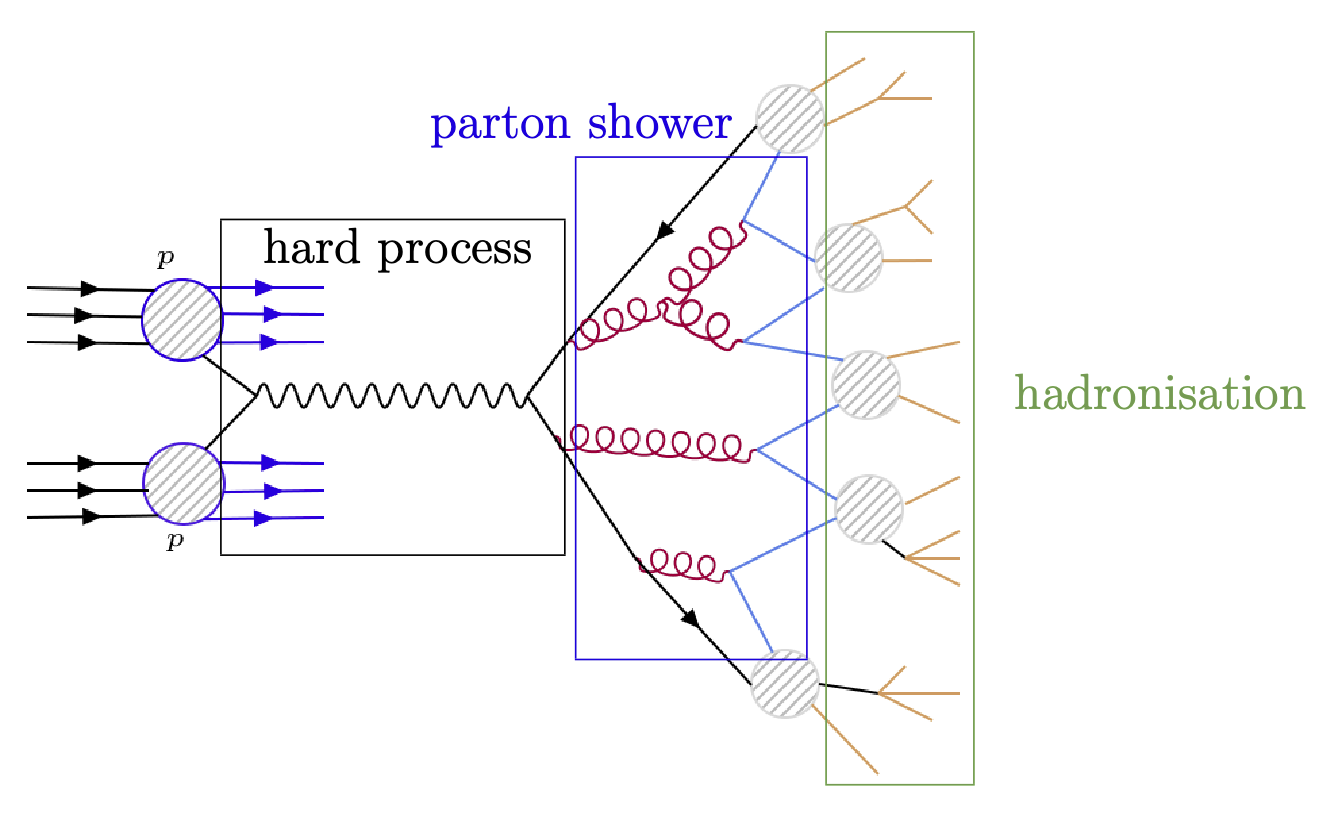
\includegraphics[width=0.8\textwidth]{plots/chapter4/simulation.png}
  \caption{Monte Carlo simulation of an event in proton-proton collisions.}
  \label{fig:simulation}
\end{figure}

In the following sections, first, the simulation of short distance processes is described. In these processes the momentum scales are high enough to use perturbative quantum chromodynamics for the description of the strong interaction between quarks and gluons. Next, quarks fragmention into composite particles called hadrons is described using the hadronization models. This is followed by soft hadron-hadron physics modelling and tuning.

First, the simulation of short distances processes is described, where the momentum scales are high enough to use perturbative quantum chromodynamics for the description of the strong interaction between quarks and gluons. Afterwards, hadronisation models are discussed which become important at lower energy scales, where quarks fragment into composite particles called hadrons. Soft hadron-hadron physics modelling, parameters and tuning are introduced. Lastly, the Monte Carlo generators that are important for the current analysis are presented along with the simulation of the detector response.


\section{Perturbative simulation}

The primary hard interaction process along with the decay of short-lived particles happen at short-distance scales. The QCD and quantum electrodynamics (QED) radiation at time scales much below $\frac{1}{\Lambda}$, where $\Lambda$ is a typical hadronic scale of a few hundred MeV are also happening at short-distance scales. Soft- and collinear-safe inclusive observables, such as total decay widths or inclusive cross sections, can be computed with pQCD theory for momentum scales much larger than this scale. The final-state collinear splittings and soft emissions give rise to large logarithmically divergent corrections which cancel against virtual corrections in the total cross section. Initial state collinear singularities are factorised into parton density functions (PDFs). Therefore the crosssection for the process remains accurate up to higher order corrections if it is interpreted as inclusive crosssection. If this is not the case then the singularities in QCD can lead to a non-convergence of the fixed-order expansion.

Matrix-element generators generate the matrix element of the hard process and large-angle emissions. The parton showers are generated by hadronic event generators using collinear and soft radiation approximations. Parton-level events are transferred from a hard-process generator to a shower generator, containing a list of particles and the used free parameters, using the Les Houches Event File (LHEF) standard \cite{Alwall:2006yp}.

\subsection{Matrix element generators}

Matrix element generators generate the exact matrix elements for the production of the process. They also produce a certain number of additional partons for hard, large-angle emissions. The radiation of extra partons is not included at tree-level accuracy of the hard process. The radiation of an extra parton with tree-level accuracy can be included to provide Next-to-leading order (NLO) corrections along with all NLO virtual corrections. The parton shower algorithms use as input the final-state partons of the hard process and their phase space.

\subsection{Parton shower algorithm}

The parton shower algorithm is used for computing the cross section for a generic hard process. The kinematics of the basic process are first generated, followed by a sequence of independent shower splittings. Sudakov form factors $\Delta_{i}(t, t')$ \cite{Collins:1989bt}, are used for estimating the probability for undergoing a branching before the infrared cut-off for each primary process parton i. The infrared cut-off is defined by the decay width for an unstable particle or the shower hadronization scale. Sudakov form factor is interpreted as the probability for a splitting not to occur between two scales $t < t'$. The parton is either split into two partons or the parton is defined as final parton. Altarelli-Parisi splitting kernels \cite{Altarelli:1977zs} define the probability of the parent parton i, with energy fraction z, to decay into two partons j and k. All generated partons undergo this procedure recursively and the algorithm stops when no final-state parton undergoes further splitting.

At each splitting vertex we can assign the azimuthal angle $\phi$ of the splitting process with respect to the incoming parton momentum, the energy fractions $z$ of the two partons, and an ordering variable for the purpose of ordering the parton splittings. PYTHIA uses the imparted transverse momentum $p_{\perp}$. The cross section for the given final state is calculated by assigning a probability to each splitting vertex. Collinear emission and emissions of soft gluons at arbitrary angles are the two sources of infrared singularities in massless field theories like QCD. PYTHIA uses a $p_{\perp}$-ordered shower evolution for correctly describing both effects. There is also an angular veto to avoid the particle multiplicity growing too rapidly with energy.

A cut-off for collinear radiation is obtained from quark masses larger than $\Lambda$, like c, b, or t quarks. For angles between both produced partons $\theta < \theta_{0} = \frac{m_q}{E}$, where $m_q$ is the quark mass and $E$ is the energy, the divergent behaviour is regulated. Heavy quarks have less collinear activity than light quarks. Therefore, in the hard process a larger fraction of the momentum acquired is carried by them. A matrix-element correction method is used by PYTHIA to include the mass effects. PYTHIA does not take the spin correlations into account when generating the parton showers. The initial-state radiation (ISR) has to be taken into account and it induces a nonvanishing transverse momentum of the particles in the matrix element. ISR is taken into account using backwards evolution algorithms.

Photon emission from light charged particles are also added by shower algorithms to account for electromagnetic corrections. For electrons, soft photon emission is especially important. A cut-off for the electromagnetic shower is used to terminate the algorithm. This cut-off is the electron mass in the case of electrons and for quarks, the photon wavelength has to be smaller than the typical hadronic size of about 1 fm. Additional bremsstrahlung can be produced from hadron and tau decays involving charged particles.

The production and decay of particles are treated as being factorisable. The distribution of the mass along with the distributions of its decay products are relevant. A $\delta$ function at pole mass $m_0$ or a Breit-Wigner distribution with particle width $\Gamma$ can be used for mass distribution. Differential decay matrix elements or the pole mass and a uniform phase-space distribution can be used for describing the decay products. The total invariant mass of the decay products is preserved by most parton-shower models to keep the original resonance shape.

\subsection{Matching}

QCD color confinement restricts quraks and gluons from existing as isolated particles. The hadronisation of a quark or a gluon gives rise to hadrons or their decay products. Jets are collimated bunches of these hadrons. The collinear/soft-radiation of an appropriate (N + 1)-parton final state, generated by a matrix element generator, can give rise to a (N + 1)-jet event. A (N + 1)-jet event can also be obtained from an N-parton final-state with hard, large-angle emission during shower evolution. A matching has to be done if different generators have been used for generating matrix-elements and parton showers or extra partons have been generated by the hard-process generator.

The exact matrix elements for the production of the basic process and up to n partons are generated by the matrix element generator. At large angles they are tree-level accurate and match the results of the shower algorithms at small angle. The relative transverse momentum is above a scale $Q_{cut}$ for each produced parton pair. There are no final states with more partons and no emissions below the scale $Q_{cut}$.

The hadronic event generator generates events with less than these n additional partons and splittings for scales below $Q_{cut}$. Splittings are also generated for initial events with n partons for relative transverse momenta below the scale of smallest pair momentum $Q_{cut}$. For fixed-order perturbation theory to hold, the matching parameter $Q_{cut}$ has to be large enough. However, the $Q_{cut}$ also has to be small enough so that the shower algorithm is accurate for emissions below it. Consistent coupling constant, \as, choices between real and virtual corrections have to be used.

To avoid phase-space double-counting as well as unpopulated phase-space regions matching schemes \cite{Hoche:2006ph} are used. These schemes define which of both paths should be generated for a given event. The choice of the path is optimised to use the best possible approximation to given kinematics. For the production of final state X and n jets, a jet measure is defined and all cross sections are calculated. Hard parton samples are then generated with a probability according to the total cross section and the matrix element. A dynamical, kinematics-dependent probability is used to accept or reject the events. The parton shower is finally invoked and no extra jets are produced with it.


\section{Hadronisation models}

The hadronisation scale $Q_{had}$ is by construction equal to the infrared cut-off where the parton shower ends. Coloured partons are transformed into a set of colourless hadrons by GPMCs. This happens at scales with low momentum transfers and at long distances, where non-perturbative effects become important. QCD inspired models which rely on the colour-flow information between partons are used by GPMCs as starting point for hadronisation. The probability distribution for the hadron energy fraction from coloured partons is given by fragmentation functions.

\subsection{Fragmentation function}

Fragmentation functions are probability distributions for inclusive hadron spectra. They can be calculated using pQCD and a non-perturbative initial condition obtained by fitting hadron spectra and are defined at an arbitrary perturbative scale Q. More information is included in the MC modelling and is exclusive, while the fragmentation function only describes inclusive spectra \cite{Peterson:1982ak}.

\subsection{String model}

String models are based on ``linear confinement''. In quenched lattice QCD, at distances greater than a femtometre the potential of the colour-dipole field between a colour charge and an anticharge appears to grow linearly with charge separation. One such model os the Lund model. Parton showering gives rise to color-connected quark-antiquark pairs. As the string grows, the non-perturbative creations of new quark-antiquark pairs are favoured, which break the string in two new strings. Kinks are used for representing intermediate gluons which can also be involved, building a transverse structure in the one-dimensional object, while innitely soft gluons are absorbed into the string. When a string breaks they are causally disconnected.

In the Lund model, starting with the leading hadrons the string breaks are generated, containing the endpoint quarks, iterating inwards to the centre of the string, alternating between both sides. In each step, a single on-shell hadron can be split off. After the breakup process the quarks can acquire a transverse momentum $p_{\perp}$. $m_{q}$ and $p_{\perp}$ are used for exponentially suppressed production of quarks. Strangeness can be generated in the parton shower through perturbative $g \to s\bar{s}$ splittings. Baryons can be produced by allowing string breaks to a pairs of diquarks. The relative rate of diquark to quark production can be extracted from collision measurements of ratio of proton to pion.

The produced quarks are assigned to hadron multiplets. As the individual rates are not predicted by the model there are many free parameters. The ratio of vector to pseudoscalar production is another parameter. The fraction $z$ of the quark longitudinal-momentum carried by the created hadron is estimated using the Lund symmetric fragmentation function. Heavier flavoured hadrons carry a larger momentum fraction $z$ of the heavy quark \cite{Bjorken:1977md}, therefore their fragmentation functions should be harder than a light hadron.

\subsection{Hadron and tau decays}

Many primary hadrons originating from string breaks are unstable and decay further until a set of particles is obtained which is stable on relevant time scales. The final particle yields and spectra have a significant impacts from the decay modelling. The summary of available experimental measurements are represented in particle summary tables. Charmed hadron decays have been measured at different experiments and all measured branching ratios do not have to sum to unity. However, MC simulations need decay packages with quantified, consistent information, with all branching fractions adding up to unity. Hence, choices have to be made when adapting summary tables and double counting has to be avoided. The differential distribution of the decay products in phase space also needs to be decided. For a selected class of decays matrix elements can be used. It depends on the generator if additional effects, such as B-meson oscillations, or CP-violating effects, are included.


\section{Soft hadron-hadron physics modelling}

Underlying Event (UE) is the additional activity beyond the basic process and its associated ISR and FSR activity. The dominant part is coming from additional colour exchanges between the beam remnants. Multiple parton-parton interactions (MPI) can produce two or more back-to-back jet pairs with each pair having a small transverse momentum. This is in contrast to jets coming from bremsstrahlung which tend to be aligned with their parent parton. Most MPI are soft and they influence the colour flow and the total scattered energy of the event. This increases the the particle multiplicity in the final state and affects the final-state activity. Compared to events with no hard jets, the hard jets appear to sit on top of a higher "pedestal" of underlying activity. This comes from the impact parameter-dependence, since central collisions are more likely to contain at least one hard scattering due to the higher probability of interactions and is called the "jet pedestal" effect. Therefore, the impact-parameter shape is another free parameter.


\section{Parameter Tuning}

The accuracy of the used models is very important for event simulation. The accuracy depends on the inclusiveness of the chosen observables and on the sophistication of the simulation. The models can be improved by improving the theoretical calculations. The precision also depends on the constraints in the free parameters and existing collision data is used to constrain them and is referred to as generator tuning. MC generators are not tuned beyond the constraints in theoretical and experimental precision due to overfitting. Otherwise it would describe fluctuations or noise instead of the underlying relationship. PDFs for the evolution probability for ISR, \as, properties of non-perturbative fragmentation functions, the matching parameter Qcut and the hadronisation scale Qhad are the parameters. Other parameters are the production rates of mesons and baryons, including the ratio of vector to pseudoscalar production, their masses and decay widths. The largest amount of free parameters are from these parameters and the parameters of the decay modelling. If significant changes to decay treatment are made then the hadronisation parameters should be retuned. As discussed for the underlying event activity and the jet-pedestal shape, the impact parameter shape of the beam particles is an important parameter. The final state y the particles and their spectra are influenced by event modelling and the generator tuning. Events generated with different generators or tunes can be different and might not describe the collision data in the entire phase space.


\section{Monte Carlo generators}

GPMC generators like PYTHIA can simulate the full process. However, there are specialized generators which deal with a certain aspect of the event simulation. MadGraph 5 generates the matrix element with leading-order (LO) accuracy \cite{Alwall:2011uj}. MadGraph 5 is a matrix element generator for processes that involve final states with a large number of jets, heavy flavor quarks, leptons and missing energy. Events from new physics models which are renormalisable or from an effective field theory that can be written in form of a Lagrangian can be generated. The Feynman rules from a given input Lagrangian are derived using FeynRules \cite{Christensen:2008py}. The Feynman diagrams are generated and the code is computed which is necessary to evaluate the matrix element at a given phase-space point for a process using the Feynman rules. Valid diagrams are constructed by the diagram generation algorithm which recursively generates all diagrams in parallel reusing already calculated subdiagrams. Wave functions can be reused when they correspond to identical subdiagrams, but contribute to different diagrams. For each fermion line in a diagram, a fermion flow is defined. Fermions are grouped in pairs with each constituting a fermion line. For states which are charged under SU(3)C, the color coefficients in scattering amplitudes are computed. Multiparton amplitudes are important as they correspond to leading order approximation of multi-jet production. The full amplitude is split into gauge invariant subamplitudes. The matrix element that results contains the full spin correlation and Breit-Wigner effects, but are not valid far from the mass peak.

POWHEG is a framework for implementing next-to-leading order (NLO) matrix-element calculations \cite{Alioli:2010xd}. It includes NLO virtual corrections and radiation of an extra parton in the matrix element. POWHEG method has been applied to several hard processes, including single top production, \ttbar production and Higgs production via gluon fusion, vector boson fusion, and Higgs boson fusion production associated with a vector boson (Higgs strahlung). It needs the LO matrix-elements and the finite part of the virtual corrections as input from which it finds all the singular regions. Using the Frixione, Kunszt and Signer (FKS) subtraction scheme \cite{Frixione:1995ms, Frixione:1997np} the real cross section is split into a sum of contributions that are divergent in one singular region. The singular regions are characterised by final-state parton becoming collinear or soft to either an initial-state parton or a final-state parton. The singular regions can be grouped according to their underlying LO-diagram by replacing this parton pair with a single parton of appropriate flavor. Soft and collinear counterterms as well as remnants are built after finding all singular regions. The POWHEG Sudakov form factor are used for generating the radiation. When no radiation is generated, Born-like events are generated. Below a threshold gluon splittings into heavy quark pairs are avoided. The incoming and outgoing partons are assigned color on basis of the underlying LO-process and to the real emitter and the radiated parton. Since the resonance mass must be preserved by the shower, the information on intermediate resonances is made available to the shower program along with the decay products being specied. The flavor structure has one more light parton in its final state and colourless and massive coloured particles remain the same at LO and NLO level. The interference of LO and one-loop amplitude, have the same flavor structure as the LO term.

aMC@NLO implements all aspects of NLO computation and its matching with parton showers \cite{Frederix:2011ss, Alwall:2014hca}. NLO calculations can be achieved by combining the computation of one-loop matrix elements and tree-level matrix elements. Tree-level computations are performed using MadGraph and one-loop amplitudes are evaluated with MadLoop \cite{Hirschi:2011pa}. The undesirable large short-scale effects can be removed by MC counterterms. They also set an upper bound for the hardness of each branching. Matched samples, which differ by their final-state multiplicity, can be merged using the FxFx- merging scheme.

MLM matching scheme is a matching algorithm \cite{Mangano:2001xp, Mangano:2002ea} that matches partons from matrix element calculations to jets reconstructed after shower generation. Parton-level events are required to have a separation greater than a minimum value $R_{jj} > R_{min}$ between them and at least a minimum transverse energy $E^{min}_{T}$ for partons. These events do not any hard-emission veto during shower. Starting with the hardest parton, the jet closest in $(\eta, \phi)$ is selected and both match if the distance is smaller than $R_{min}$. Once a match is found the jet is removed and matching is done with the next parton. If a match is not found then the event is rejected. This is the case for collinear partons or soft partons, which do not lead to an independent jet or are too soft for jet reconstruction.

FxFx merging scheme is an NLO merging procedure \cite{Frederix:2012ps}. There can be NLO accuracy for exclusive events with J light jets by the computation based on matrix elements that have J and (J + 1) partons. NLO mergings are more complicated than LO ones. This is because the matrix elements are considered twice, as Born contribution for processes with J partons, and as real-emission contribution, IR subtraction terms, and the one-loop contributions to a processes with (J - 1) partons. Double counting is avoided by parton-shower dependent MC counterterms and Sudakov reweighting, as Sudakov form factors include virtual corrections and non-emission probabilities. The parton shower dominates at soft scales, while the contributions from the matrix element dominate at hard scales. At intermediate scales a probability function estimates which description is more accurate. There is no emission larger than the matching scale generated by shower. Events are reweighted and a certain amount of events might carry negative weights.

PYTHIA 8 has been developed for multiparticle production in $e^{+}e^{-}$, $pp$ and $ep$ collisions and simulation of jets. PYTHIA can generate the hard subprocess, initial- andnal-state parton showers, hadronisation, decays and the underlying event. A lot of hard processes have been implemented for generating the matrix elements for final-state and phase space calculation. $2 \to 1$ and $2 \to 2$ processes can be optimally generated by PYTHIA. Resonance decays with the resonance masses above the b-quark system are implemented. Their branching fractions and partial width can be dynamically calculated as function of their mass. If the spin information is available for resonance decays it leads to properly correlated angular correlations of the resonance decay products, otherwise the resonance decays isotropically.

A multijet structure is added by the parton shower which does not take into account the spin effects. Showers are ordered by their virtuality $p_{\perp}$. The initial-state showering is done by a backward evolution scheme. The shower is traced backwards in time starting from the incoming parton of the hard interaction to find the parton which initiated the shower. PYTHIA 8 uses Dipole showering. Gluon emission is generated via dipole radiation rather than by splitting partons. FSR are associated with dipoles which are stretched between the "hole" left by an initial-state parton and a final-state parton. The hard scattering subsystem takes the recoil having initial-state radiation unchanged. Lund string model is used for implementing the Hadronization. The process is split into generating the fragmentation and the decays of these hadrons.


\section{Detector simulation}

In detector simulation, the interactions of particles with the detector material and the detector response are simulated. These events can then be reconstructed and analysed. Geant4 \cite{Agostinelli:2002hh} is used for detector simulation. It is a toolkit for simulating passage of particles through matter and for simulating particle interactions with matter across a very wide energy range. The user defines the detector geometry and materials. A large number of components with different shape and materials can be included in the geometrical model. Sensitive elements can be defined which record information in the form of hits. Hits are needed to simulate the detector responses called digitisation. The detector's geometrical structure is divided into logical and physical volumes. Logical volumes contain the information of the material and the sensitive detector behaviour. A mixture of different elements and isotopes can be used for the material. Physical volumes carry information about the spatial positioning or placement of the logical volumes.

Particles can interact with the detector material or can decay while they are transported through the geometry. A model can be implemented by electromagnetic and hadronic processes in Geant4 depending on the energy or particle type. Geant4 can handle ionisation described by energy loss and range tables, bremsstrahlung, pair production of electron-positrons from muons, photo-electric effect, pair conversion, annihilation, synchrotron and transition radiation, scintillation, refraction, reflection, absorption, the Cherenkov effect, and many other processes. Particles with their basic properties, like mass, charge, list of sensitive processes, can be defined. Particles are transported in steps and they are tracked through materials and external electromagnetic fields. Event data is generated during simulation. First, events contain primary vertices and primary particles before processing an event. After processing, hits and digitisations generated by simulation are added. Trajectories of simulated particles can be added optionally for recording of "simulation truth".

%
% Chapter 5
%

\chapter{Event reconstruction}
\label{event_reco}

The particle-flow (PF) event reconstruction aims to reconstruct and identify each particle in an event with an optimized combination of information from the various CMS detector elements~\cite{Sirunyan:2017ulk}. In this process, identifying the PF candidate type (photon, electron, muon, charged, and neutral hadrons) plays a vital role in determining particle direction and energy. The PF algorithm links several PF elements that a physics object can give rise to across different sub-detector layers. The PF elements are tested for their compatibility in the $\eta$--$\phi$ plane and are combined to form PF blocks. A predefined sequence of reconstruction and identification algorithms are run in each of these PF blocks. This sequence starts with the reconstruction and identification of muon candidates. PF quality criteria are placed for the muon candidate. The PF elements associated with a muon candidate passing these criteria are removed from the block. The next step in the sequence is to reconstruct and identify electron candidates. The electrons are defined as PF electrons if the tracker's extrapolated tracks have a corresponding energy deposit in the ECAL. The sequence now proceeds with identifying photons and hadrons. In the sequence, tracks with momentum uncertainty more than the calorimeters' resolution are removed to reduce misidentified tracks. All the remaining tracks are associated with charged hadrons, and all the remaining calorimeter energy deposits are associated with photons (ECAL) and hadrons (HCAL). At the end of this sequence, we are left with a list of all electrons, photons, muons, charged hadrons, and neutral hadrons in the event with optimally determined direction, charge, and energy.


\section{Track and primary vertex reconstruction}

The hits from the pixel and strip detectors in the tracker are used to reconstruct the tracks of charged particles~\cite{Chatrchyan:2014fea}. Signals above specified thresholds in the pixel and strip channels are clustered to form the hits. The cluster positions and corresponding uncertainties are estimated in a local orthogonal system plane of each sensor. A translation is done between the local coordinate system of these hits to the tracks' global coordinate system during track reconstruction. Kalman filter (KF)~\cite{Fruhwirth:1987fm} based algorithm is used to reconstruct tracks and is called the combinatorial track finder. Tracks with high \pt and those produced near the interaction region are easiest to find. Track reconstruction uses an iterative procedure with the initial iterations searching for the most accessible tracks. In subsequent iterations, tracks with low \pt and those produced far from the interaction region are searched. Hits unambiguously assigned to the track in the previous iterations are removed. This reduces the combinatorial complexity in the subsequent iterations. In each iteration, there are four sequential steps.

The first step in the sequence is seed generation. The magnetic field causes the charged particles to follow a helical path, requiring five parameters to determine the trajectory. These parameters are extracted using two or three hits in the inner region of the tracker. The seeds are constructed in the inner part owing to the high granularity of the pixel detectors. The tracks are then constructed outwards. The motivation to use the inner region for seed construction also rests on the fact that particles like pions and electrons interact inelastically with tracker material as they traverse through the tracker to its outer regions.

KF based algorithm is then used for track finding. Track parameters are estimated by using the trajectory seeds generated in the previous step. The seed trajectories are extrapolated along the expected path of a charged particle. The track candidates are built using the location and uncertainty of detected hits, taking into account effects such as Coulomb scattering at successive detector layers. The parameters are updated at each layer. An analytical extrapolation is done that determines which adjacent layers of the detector the trajectory can intersect. A search is performed for silicon modules in these layers that are compatible with the extrapolated trajectory. Mutually exclusive groups are built from all compatible modules in each layer such that no two modules in each group overlap. One of the compatible hits from a group of hits is added to the original track candidate to form new track candidate. The added hits' information is combined with the original track candidates' extrapolated trajectory to update the new candidates' trajectory parameters. Figure~\ref{fig:trackeff} illustrates the reconstruction efficiency of tracks in the case of isolated muons.

The hits from the last step are refitted using a KF in a phase called track fitting. This provides the best possible estimate of parameters for each track trajectory. There can be several misidentified tracks that are not associated with any charged particle passing through the tracker. Several quality requirements are applied to the set of reconstructed tracks, which substantially reduces the misidentified tracks contribution. The quality criterion involves the minimum number of layers the track has hits in, how compatible its origin is with a primary vertex (PV), and how good a fit it yields.

The interaction vertices in the \pp collisions are reconstructed by selecting tracks produced promptly in the primary interaction region. The chosen tracks are clustered based on their z-coordinates at their closest approach to the beam spot center. The beam spot represents a 3-D profile of the region where the proton beams collide inside the CMS detector. The adaptive vertex fitter procedure is used for finding the exact positions of the vertices from these clustered candidates~\cite{Fruhwirth:2007hz}. The PV has the most significant sum of squared transverse momenta of tracks originating from it.

\begin{figure*}[!htpb]
  \centering
  \captionsetup{width=0.98\textwidth,justification=centering}
  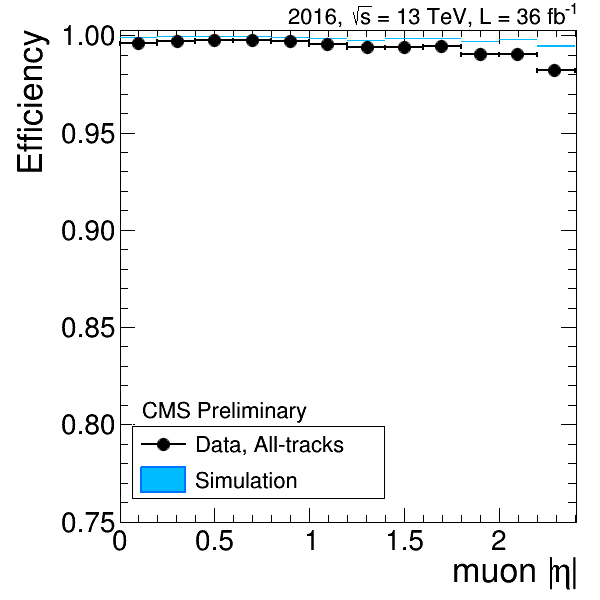
\includegraphics[width=0.45\textwidth]{plots/chapter5/TrackEta2016.png}
  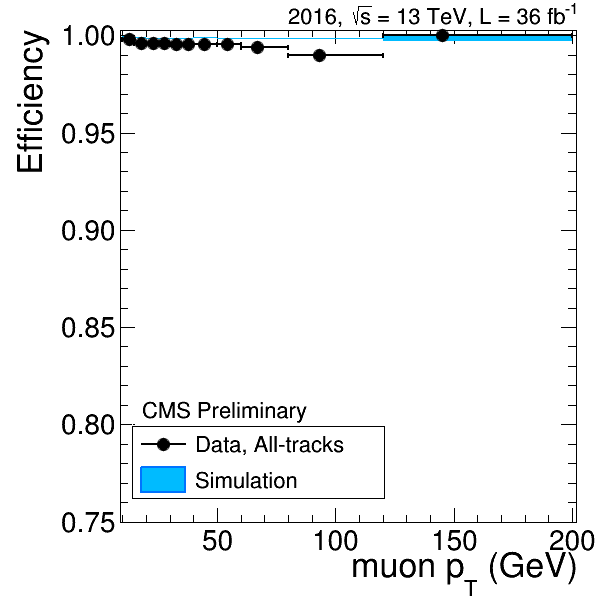
\includegraphics[width=0.45\textwidth]{plots/chapter5/TrackPt2016.png} \\
  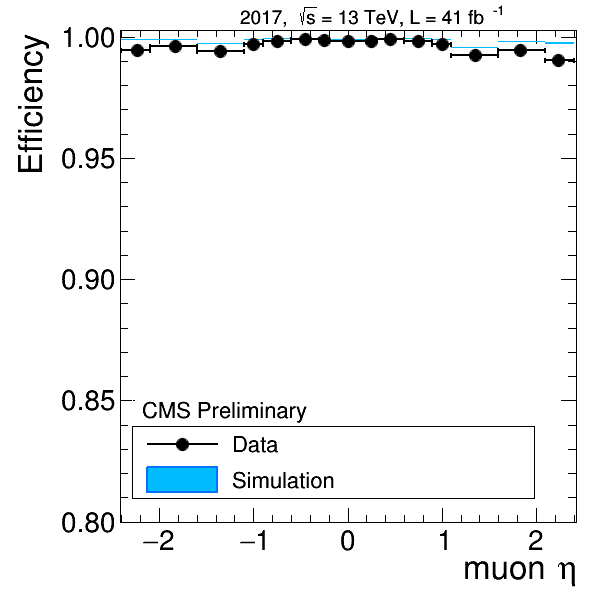
\includegraphics[width=0.45\textwidth]{plots/chapter5/TrackEta2017.png}
  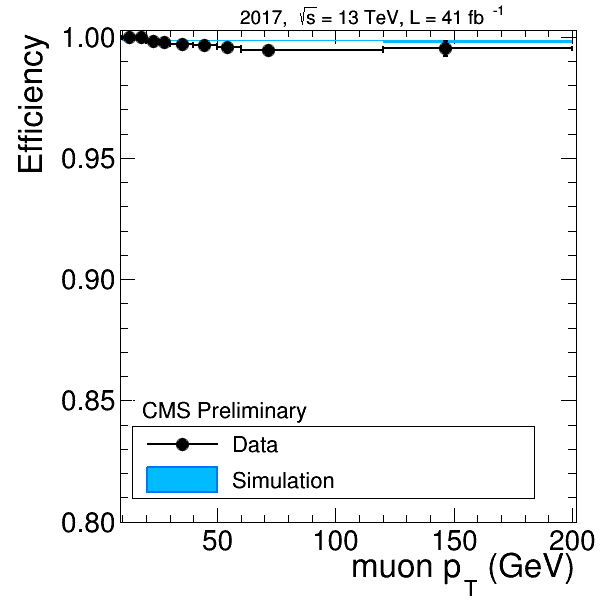
\includegraphics[width=0.45\textwidth]{plots/chapter5/TrackPt2017.png} \\
  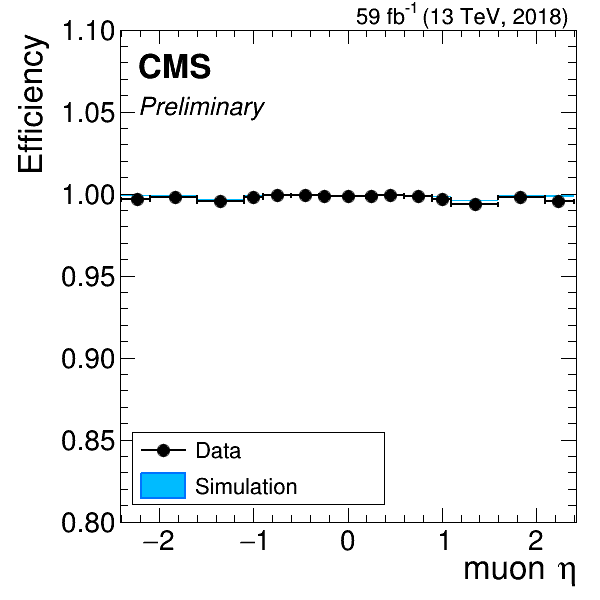
\includegraphics[width=0.45\textwidth]{plots/chapter5/TrackEta2018.png}
  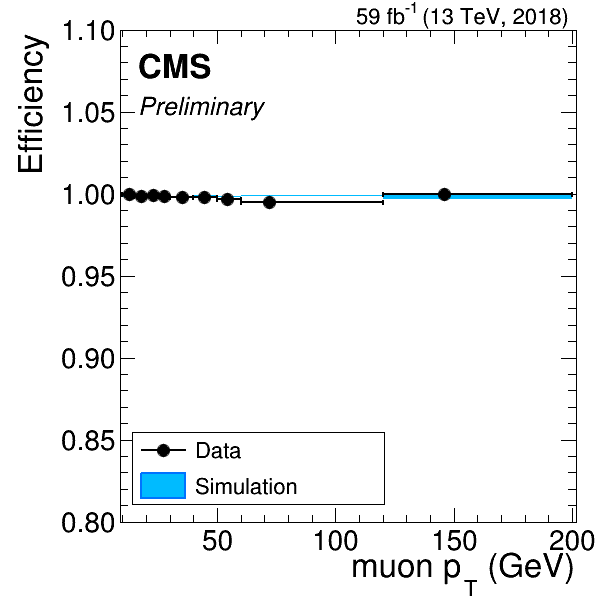
\includegraphics[width=0.45\textwidth]{plots/chapter5/TrackPt2018.png} \\
  \caption{The tracking efficiency for ``all-tracks'' collection as a function of pseudorapidity and transverse momentum for muons coming from the \PZ decay.}
  \label{fig:trackeff}
\end{figure*}


\section{Muon reconstruction}

Muons are reconstructed using the hits in the muon system, and tracks from the tracker~\cite{Sirunyan:2018fpa}. The gas in the muon chambers is ionized when muons traverse through them. The ionization is read-out by electronics systems that associate these ``hits'' with well-defined locations in the detector. The hits in the muon chambers are reconstructed independently of track reconstruction in the tracker. KF is used for reconstructing the hits from the muon system. These tracks are called standalone-muon tracks. Tracker tracks with $\pt > 0.5 \GeV$ are propagated to the muon system. Muon tracks are built from these tracks by matching them to segments of hits in DT or CSC. A matching tracker track is called a tracker muon track. Standalone-muon tracks can be matched with tracker tracks and combining information from both using a KF fit. The muon tracks built in such a manner are called global muon tracks. Muons leaving hits in several muon stations have a very efficient global muon reconstruction. Muon candidates with low \pt have an efficient tracker muon reconstruction. However, it can cause misidentified muon tracks due to hadronic particles, which punch-through to the innermost muon stations. The global muon reconstruction reduces the muon misidentification rate compared to tracker muons. The efficiency for reconstructing a muon is as high as 99\% when tracker muon tracks and global muon tracks are combined. PF algorithm applies the quality criterion for the reconstructed muon candidates. The PF muon candidates used in the analysis were required to satisfy the following set of criterion to be identified as a muon:

\begin{itemize}
  \item The candidate is reconstructed as a global muon along with PF muon identification.
  \item $\chi^{2}$/ndof of the global muon track fit $< 10$.
  \item At least one muon chamber hit included in the global muon track fit.
  \item There should be muon segments in at least two muon stations. This implies that the muon is also an arbitrated tracker muon.
  \item Its tracker track has transverse impact parameter $|\text{dxy}| < 2~\mm$ with respect to the PV.
  \item The longitudinal distance of the tracker track with respect to the PV is $|\text{dz}| < 5~\mm$.
  \item Number of pixel hits $> 0$.
  \item Number of tracker layers with hits $> 5$.
\end{itemize}

PF muon identification efficiency is illustrated using a plot from a study performed by the CMS muon physics object group in Figure~\ref{fig:muoneff}. There are differences in the efficiencies in data and MC simulation. They are corrected using a set of scale-factors applied as a function $\eta$ and \pt to adjust the simulation efficiency to match the efficiency in data.

\begin{figure*}[!htpb]
  \centering
  \captionsetup{width=0.98\textwidth,justification=centering}
  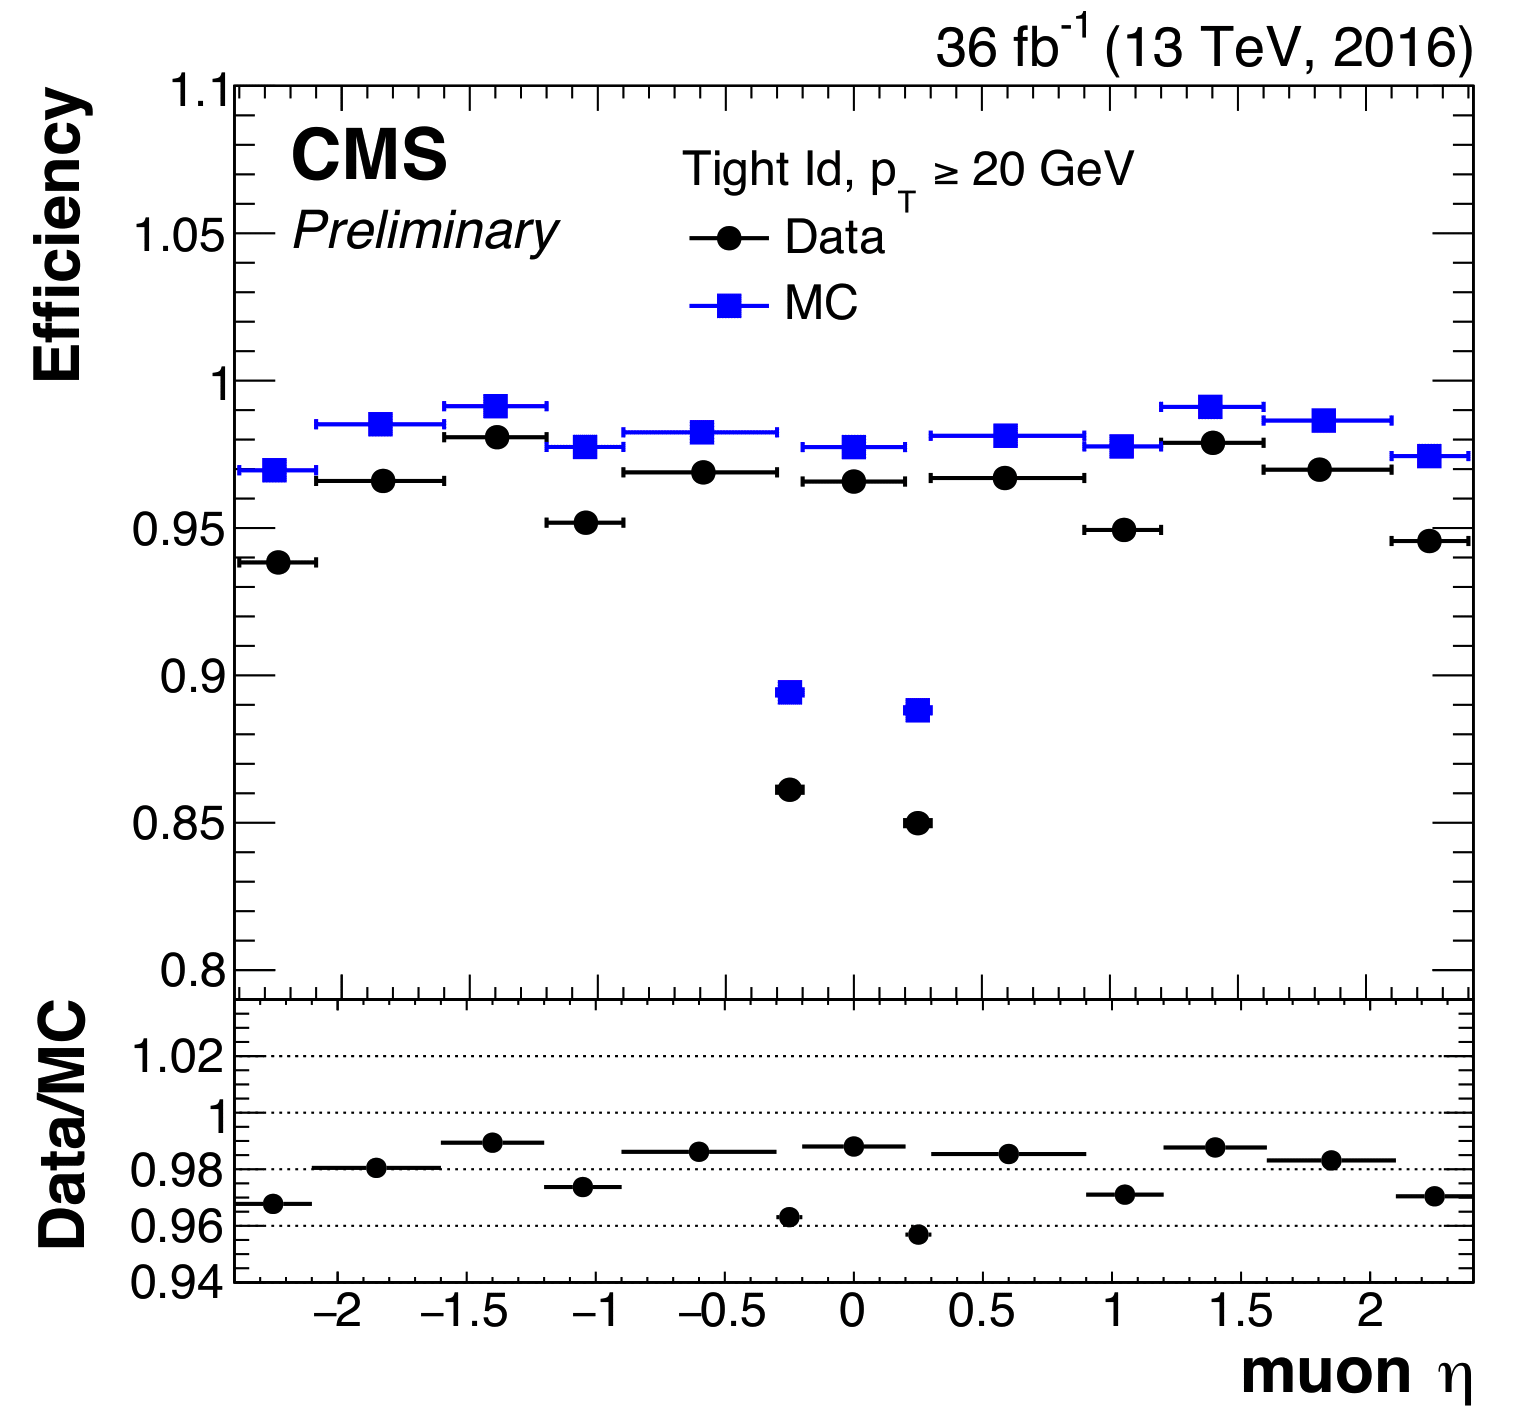
\includegraphics[width=0.49\textwidth]{plots/chapter5/Eta2016.png}
  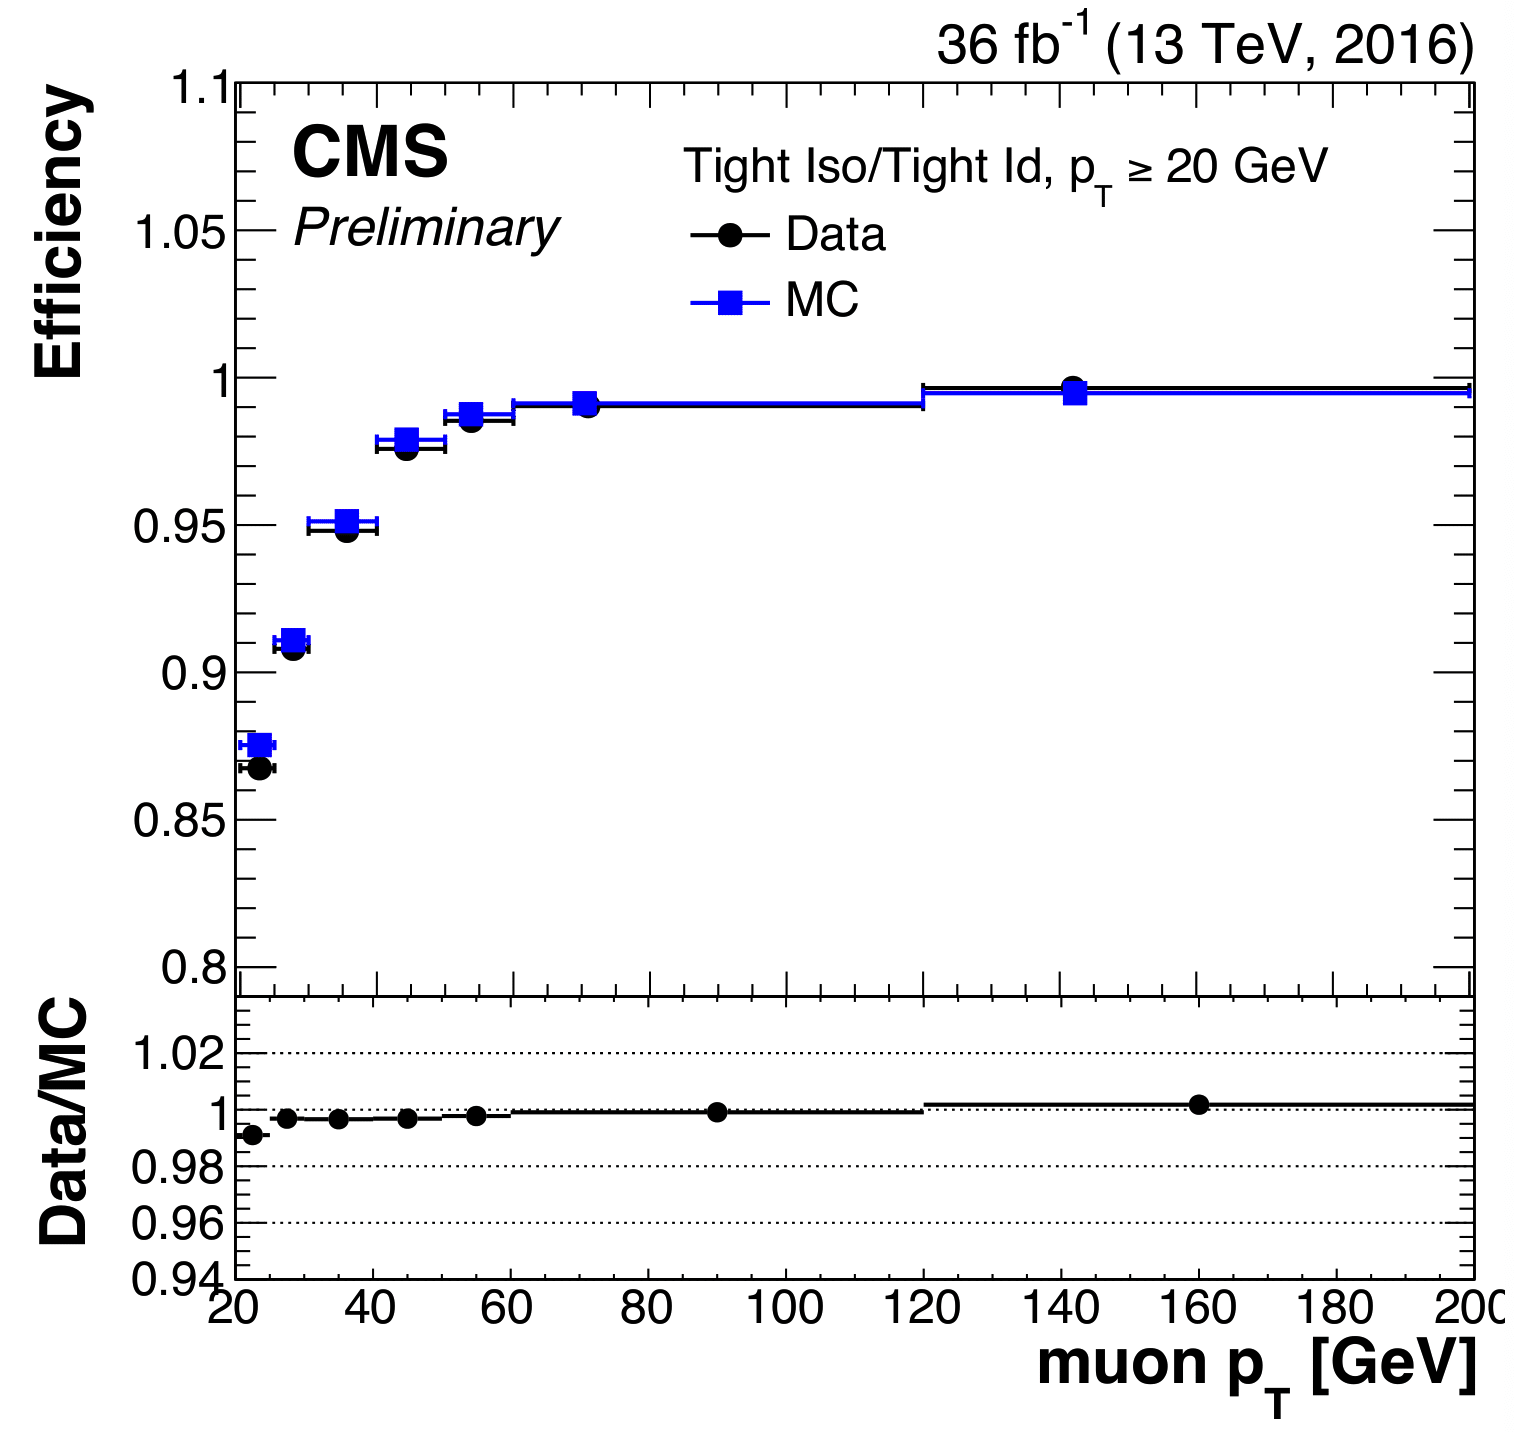
\includegraphics[width=0.49\textwidth]{plots/chapter5/Pt2016.png} \\
  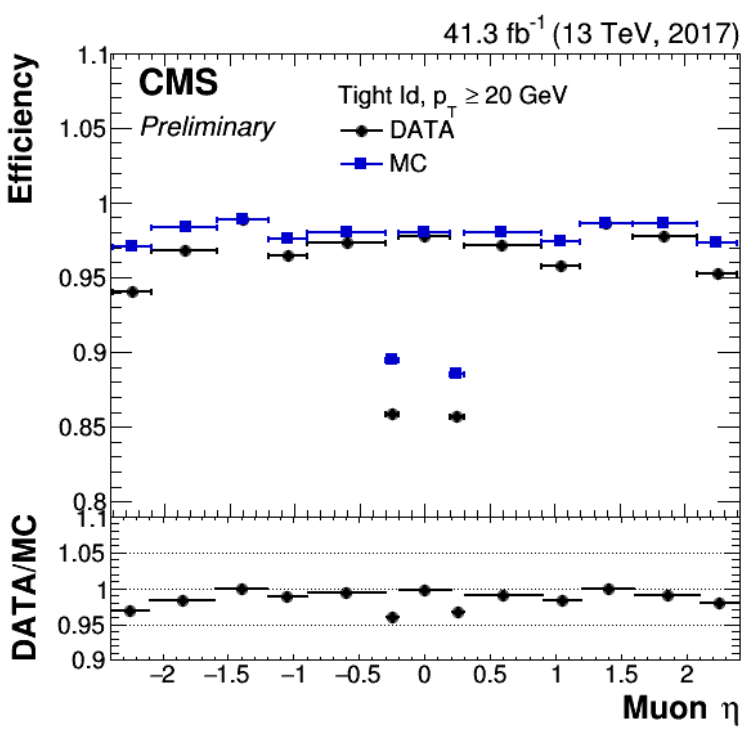
\includegraphics[width=0.49\textwidth]{plots/chapter5/Eta2017.png}
  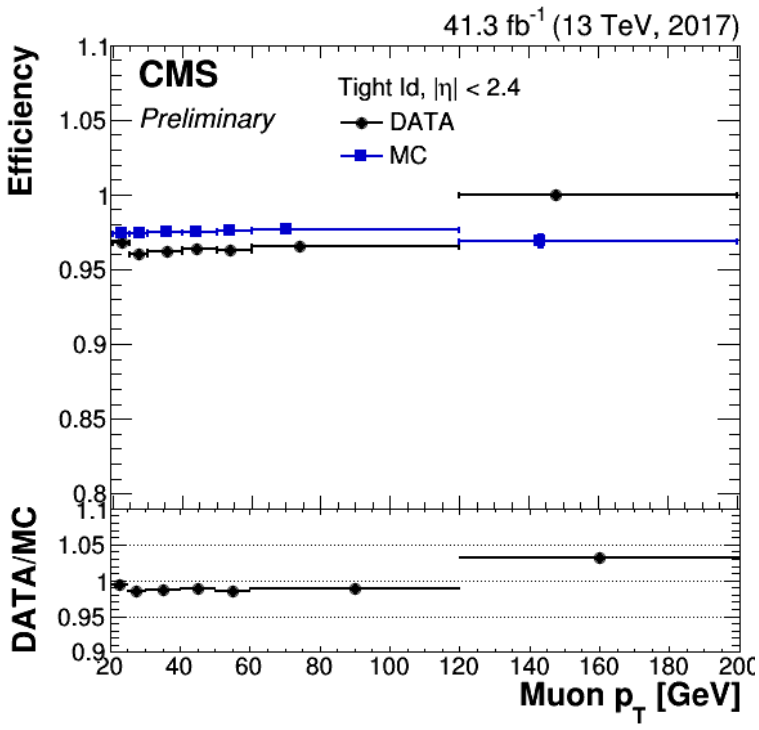
\includegraphics[width=0.49\textwidth]{plots/chapter5/Pt2017.png} \\
  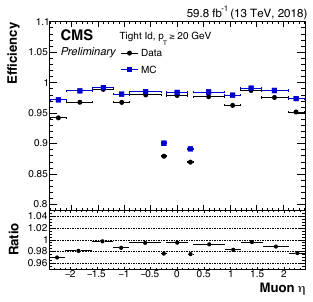
\includegraphics[width=0.49\textwidth]{plots/chapter5/Eta2018.png}
  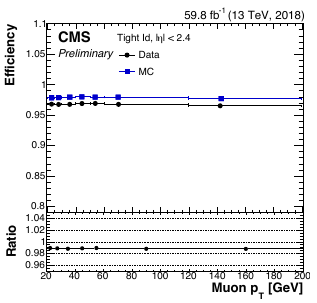
\includegraphics[width=0.49\textwidth]{plots/chapter5/Pt2018.png} \\
  \caption{Efficiency of muon identification as a function of $\eta$ and \pt, for data (black) and simulation (blue)~\cite{muon_pog}.}
  \label{fig:muoneff}
\end{figure*}


\section{Electron reconstruction}

Clusters of energy formed in the ECAL are associated with tracks from the tracker to reconstruct electrons. Electrons radiate bremsstrahlung photons caused by the interaction of electrons with atoms as they pass through the tracker. The radiation depends on the amount of detector material the electron has to cross. The clustering algorithm needs to account for these bremsstrahlung photon showers' energy to measure the electron's energy. The bremsstrahlung photons' energy spreads primarily in the $\phi$ direction, and the spread in the $\eta$ direction is relatively small.

The hybrid algorithm is used to cluster the electron energy deposit in the ECAL barrel. It uses the geometry of the ECAL to form clusters that are wide in the $\phi$ direction but are narrow in the $\eta$ direction. A seed crystal contains the most significant energy deposited in the considered region above a 1~\GeV threshold. A $5 \times 1$ array of crystals are added in $\eta\times\phi$ around the seed crystals in both directions of $\phi$ if the energy contained in the array is above the 0.1~\GeV threshold. Contiguous arrays are merged into clusters. An electron supercluster is formed from all such strip clusters, which have at least one seed strip with energy above the 0.35~\GeV threshold. A different clustering algorithm is used in the ECAL endcap due to the crystals' different geometrical arrangements. This algorithm is called the $5 \times 5$ algorithm. It starts with a seed crystal satisfying the minimum energy requirement of 0.18~\GeV. A supercluster is formed by progressively grouping clusters of $5 \times 5$ crystals around the seed crystal. The added clusters need to have energy over 1~\GeV and be within $\pm 0.7$  and $\pm 0.3$ respectively in $\eta$ and $\phi$ around the seed crystal. The energy-weighted mean of the cluster positions is taken as the position of the supercluster. The sum of the energy of all its constituent clusters is its energy. The energy from the preshower is also added to the supercluster. This is implemented by using it's most energetic cluster and it's maximum distance in $\phi$ to other clusters and extrapolating it to the preshower plane to define the spread in the preshower.

A dedicated tracking procedure is used for electron candidates that use information from the tracker and the ECAL. The first step in electron track reconstruction is seeding. The reconstructed superclusters' position and energy can constrain the trajectory of the electron through the tracker and the assumption that the electrons originated close to the center of the beam spot. The electron seeds are the hits in the first layers of the trackers compatible with these trajectories. In an alternative approach, tracks constructed by the standard tracking algorithm are extrapolated to the ECAL and matched with a supercluster. The seed collections from these two approaches are merged, leading to an increase in the seeding procedure's overall efficiency. Electron track finding and fitting phases use these seeds. The track finding procedure is adjusted to accommodate tracks that deviate from their expected trajectory because of bremsstrahlung. The penalties assigned to track candidates for passing through a tracker layer without being assigned a hit are similarly adjusted. The Gaussian sum filter (GSF) is used for the final track fit. This accounts for the fact that the energy loss of an electron traversing the tracker material is non-Gaussian. As the KF algorithm assumes Gaussian distribution, the GSF technique deals with this by approximating this non-Gaussian energy loss distribution as the sum of several Gaussian functions and performs much better than the regular fitting procedure.

The electron candidates are constructed by associating the GSF track produced by the above procedure with a supercluster in the ECAL. A geometrical matching in $\eta$--$\phi$ is used for the association for ECAL seeded candidates. A multivariate (MVA) technique that combines information from supercluster and GSF track is used for tracker seeded candidates. The electron's charge is estimated using the GSF track curvature, ECAL supercluster's relative position in $\phi$ to that of the first hit in the GSF track, and KF tracks that have common hits with the GSF tracks. This combined approach reduces the charge misidentification probability to 1.5\%. A combination of tracker and ECAL measurements is used for estimating the momentum of electrons.

Several quality criteria are placed on the reconstructed electron candidates to identify electrons. This helps in suppressing misidentified sources such as photon conversions, jets misidentified as electrons, etc. Electrons are required to pass an identification variable based on a boosted decision tree (BDT) discriminator, which uses track quality, shower shapes, and kinematic quantities. The following variables are used as input to the BDT:
\begin{itemize}
  \item Cluster shape variables $\sigma_{\ieta, \ieta}$ and $\sigma_{\iphi, \iphi}$, with \ieta and \iphi the integer label of the $\eta$ and $\phi$ of a calorimeter cell. The circularity 1 - $\frac{\text{E}_{1 \times 5}}{\text{E}_{5 \times 5}}$, with $\text{E}_{1 \times 5}$ and $\text{E}_{5 \times 5}$ the energies in a $1 \times 5$ and a $5 \times 5$ grid around the supercluster seed, respectively.
  \item Shape variable $\text{R}_{9}$ = $\frac{\text{E}_{3 \times 3}}{\text{E}_{\text{SC}}}$, with $\text{E}_{3 \times 3}$ the energy in a $3 \times 3$ grid of cells around the supercluster seed and $\text{E}_{\text{SC}}$ the raw energy of the supercluster.
  \item The number of valid hits in the track fit, the $\chi^{2}$ of the track fit, and the $\chi^{2}$ of the GSF track fit.
  \item The number of GSF track hits, the number of expected missing inner hits, and the result of the conversion vertex fit.
  \item The distance $\Delta \eta$ and $\Delta \phi$ between the reconstructed supercluster and the associated track at the position of the PV, and the distance in $\eta$ between the supercluster and the track at the calorimeter surface.
  \item H/E, the ratio of the hadronic energy over the electromagnetic energy in the supercluster and E/P, the ratio of the supercluster energy over the momentum of the track associated with the electron.
  \item The ratio of the energy of the electron cluster and the momentum of the associated track, evaluated at the electron cluster, and $1/\text{E}_{\Pe} - 1/\text{P}_{\Pe}$, with $\text{E}_{\Pe}$ the energy of the electron candidate and $\text{P}_{\Pe}$ its momentum.
\end{itemize}

The BDT was trained on a \PZ/\Pgg MC sample generated with MadGraph5, in 3 $\eta$ bins for electrons with $\pt > 10 \GeV$. There are two versions of the MVA available for electron identification. The first one includes the electron isolation in training and another which does not include this, and their performance is illustrated in Figure~\ref{fig:elec_BDT}. This analysis uses the version without the isolation included in the training. An additional selection of electron isolation is used. This is done so that in the \ehad channel, the misidentified lepton background can be estimated using the isolation based sideband regions. Instead of using fixed selections on the MVA score, the selections are alternatively varied exponentially with \pt to achieve a more constant efficiency of 80\%. The electrons are also subject to the same impact parameter selections as the muons: the impact parameters between the electron track (best track) and the PV are restricted as $|\text{dxy}| < 0.045$ cm and $|\text{dz}| < 0.2$ cm to ensure the electron is associated with the PV.

\begin{figure*}[!htpb]
  \centering
  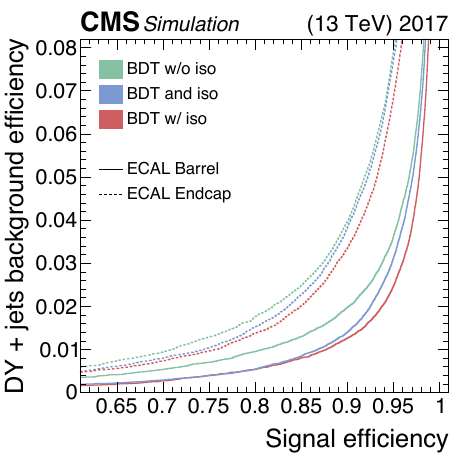
\includegraphics[width=0.5\textwidth]{plots/chapter5/BDT.png}
  \caption{Receiver operating curve showing the background versus signal efficiency for the BDT with and without isolation incorporated in training.}
  \label{fig:elec_BDT}
\end{figure*}

\section{Tau reconstruction}

Hadrons-plus-strips (HPS) algorithm is used for reconstructing the hadronic decays of tau~\cite{Sirunyan:2018pgf}. ``DeepTau'' based identification is used for discrimination of hadronic decays of tau against jets, electrons, and muons. A detailed description of the HPS algorithm, followed by the DeepTau identification algorithm, is given in the following subsections.

\subsection{Hadrons-plus-strips}

The HPS algorithm is seeded by jets clustered with the anti-\kt algorithm with a distance parameter $\mathrm{R} = 0.4$. To reconstruct the energy deposits \Pgpz candidates leave in the ECAL, photon and electron constituents of the jet that seeds the hadronic tau (\tauh) reconstruction are clustered into strips. The electron or photon (not yet included in a strip) with the highest \pt is used to build a new strip. The $\eta$ and $\phi$ of this candidate determine the initial position of the strip. The next highest \pt electron or photon within an $\eta$--$\phi$ window centered on the strip location is added to the strip. The position is recomputed as the energy-weighted average of the electron/photon constituents in the strip. This procedure is repeated until there are no more electrons or photons with $\pt > 0.5 \GeV$ within the strip window. The $\Delta \eta $ and $\Delta \phi $ of the strip vary based on the \pt or \ET to be added to the strip. It also depends on the energy, the strip already has, as
\begin{linenomath*}
  \begin{equation*}
    \begin{aligned}
      \Delta \eta = f(\pt^{e/\Pgg}) + f(\pt^{\text{strip}}) \\
      \Delta \phi = g(\pt^{e/\Pgg}) + g(\pt^{\text{strip}})
    \end{aligned}
  \end{equation*}
\end{linenomath*}
where $\pt^{e/\gamma}$ is the transverse momentum of the candidate to be added to the strip and $\pt^{\text{strip}}$ is the transverse momentum of the strip before merging a new candidate in. In addition, the strip size is bounded as 0.05 $< \Delta\eta <$ 0.15, 0.05 $< \Delta\phi <$ 0.3. The functions $f(\pt)$ and $g(\pt)$ are defined as
\begin{linenomath*}
  \begin{equation*}
    \begin{aligned}
      f(\pt) = 0.2 \cdot \pt^{-0.66} \\
      g(\pt) = 0.35 \cdot \pt^{-0.71}
    \end{aligned}
  \end{equation*}
\end{linenomath*}

If the $\pt^{\text{strip}}$ is at least 2.5~\GeV, it is considered as a \Pgpz candidate. Hadronic taus are reconstructed by combining charged particles and strips into different signatures compatible with a specific decay mode if the set of selections listed below is satisfied. If a candidate satisfies more than one of the hypotheses, the one that maximizes the \pt is retained.

The decay modes considered for reconstructing taus are:
\begin{itemize}
  \item One charged particle, no strips.
  \item One charged particle + one strip with mass $0.3 < \mt < 1.3 \cdot \sqrt{\pt/100} \GeV$. The mass window upper limit is constrained to lie between 1.3 and 4.2~\GeV.
  \item Three charged particles with mass $0.8 < \mt < 1.5 \GeV$. The tracks are required to originate within $|\text{dz}| < 0.4$ cm of the same vertex.
  \item Three charged particles and one strip with a total mass $0.8 < \mt < 1.5 \GeV$.
\end{itemize}

The reconstructed hadronic tau candidates are subject to the impact parameter selections: the impact parameter between the reconstructed hadronic tau and the PV is restricted as $|\text{dz}| < 0.2$ cm to ensure the hadronic tau is associated with the PV.

\subsection{DeepTau}

The application of machine learning techniques has been proven to provide superior results for multi-dimensional problems. DeepTau is a new multiclass tau identification algorithm based on a convolutional deep neural network (DNN)~\cite{CMS-DP-2019-033}. DeepTau combines information from the high-level variables attributed to the reconstructed \tauh candidates with low-level information from the inner tracker, calorimeters, and muon sub-detectors using PF candidates reconstructed within the \tauh signal and isolation cones. DeepTau also takes advantage of using the updated decay mode definitions.

An electron that is misidentified as a tau lepton is referred to using \taue. In contrast, a muon that is misidentified as a tau lepton is referred to using \taum, and a jet misidentified as a tau lepton is referred to using \tauj. A balanced mix of \taue, \taum, \tauh, and \tauj candidates coming from \ttbar, \wjets, and \zjets MC simulation is used to perform the training. The \tauh has a loose preselection: $\pt \in [20, 1000] \GeV$, $\aeta < 2.3$, and $|\text{dz}| < 0.2$, which makes it suitable for the current analysis. The inputs are separated into sets of high-level and low-level features. As high-level inputs, the algorithm takes variables used during tau reconstruction, and one global event variable is the average energy deposition density ($\rho$). For each candidate reconstructed within the tau signal or isolation cones, the 4-momentum, track quality, relation with the PV, calorimeter clusters, and muon stations are used.

The tau signal and isolation cones define two regions of interest in the vicinity of the tau candidate. Based on the angular distance between the reconstructed tau 4-momentum, all available candidates are split into two $\eta \times \phi$ grids of 11 $\times$ 11 (21 $\times$ 21) cells with a cell size of 0.02 $\times$ 0.02 (0.05 $\times$ 0.05) for the signal (isolation) cone. In cases where more than one object of the given type belongs to the same cell, only the object with the highest \pt is considered input. Within each cell, the input variables are split into three blocks: e-gamma, muon, hadrons.

The low-level inputs' organization into two 2D grids allows first processing the local patterns originating from the tau or jet structure. The information obtained is then iteratively combined, covering bigger $\eta \times \phi$ regions up to the point where the total tau signal or isolation cones are covered. The four outputs of the network represent estimates of the reconstructed tau candidate's probabilities to be \taue, \taum, \tauj, or a genuine \tauh. The performance of tau discrimination against quark and gluon induced jets (left), electrons (middle), and muons (right) for DeepTau and the previously available discriminators can be seen in Figure~\ref{fig:deeptau}.

\begin{figure}[hbtp]
  \centering
  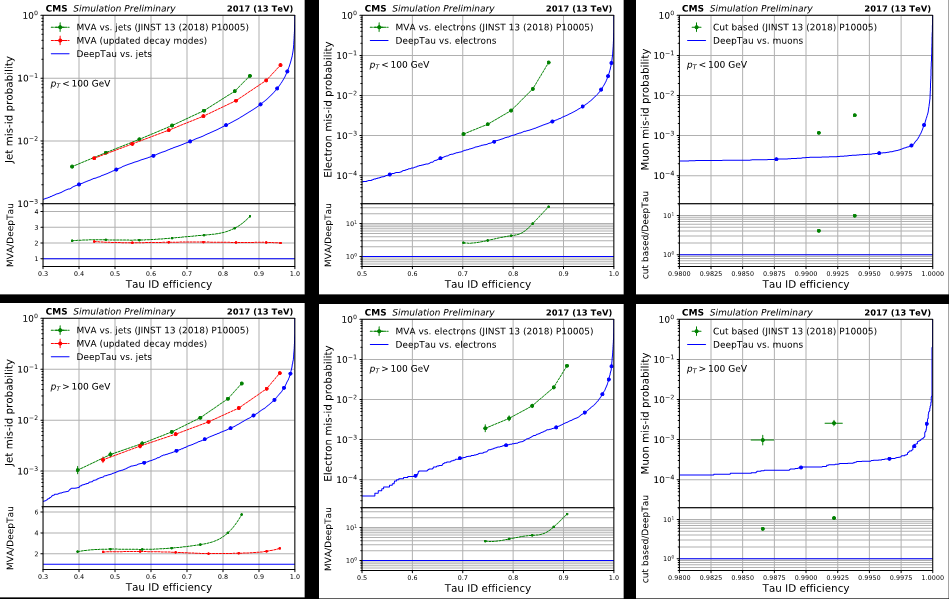
\includegraphics[width=0.98\textwidth]{plots/chapter5/deeptau.png}
  \caption{Performance of tau discrimination against quark and gluon induced jets (left), electrons (middle), and muons (right) for DeepTau and the previously available discriminators.}
  \label{fig:deeptau}
\end{figure}

A WP defined using a \pt dependent threshold on the output of the DNN is used to distinguish \tauh from jets. This WP has a \tauh identification efficiency of about 70\% with a misidentification probability of $\approx 1\%$. This helps to provide a good tau identification efficiency along with high background rejection. The DNN can reject electrons and muons misidentified as \tauh candidates using dedicated criteria based on the consistency between the tracker's measurements, the calorimeters, and the muon detectors.

In the \muhad (\ehad) channel, the WP that is used has an efficiency of about 97.5\% (87.5\%) with a misidentification probability of $\approx 1-2\% \, (0.2-0.3\%)$ to discriminate \tauh against electrons, and has an efficiency of about 99.6\% (99.8\%) with a misidentification probability of $\approx 0.04\% \, (0.06\%)$ to discriminate \tauh against muons. DeepTau identification for hadronic taus helps in reducing the \Zll($\ell=\Pe,\Pgm$) background and misidentified lepton background significantly, and the comparison with the previous analysis can be seen in Figure~\ref{fig:collmass}.

\begin{figure}[hbtp]
  \centering
  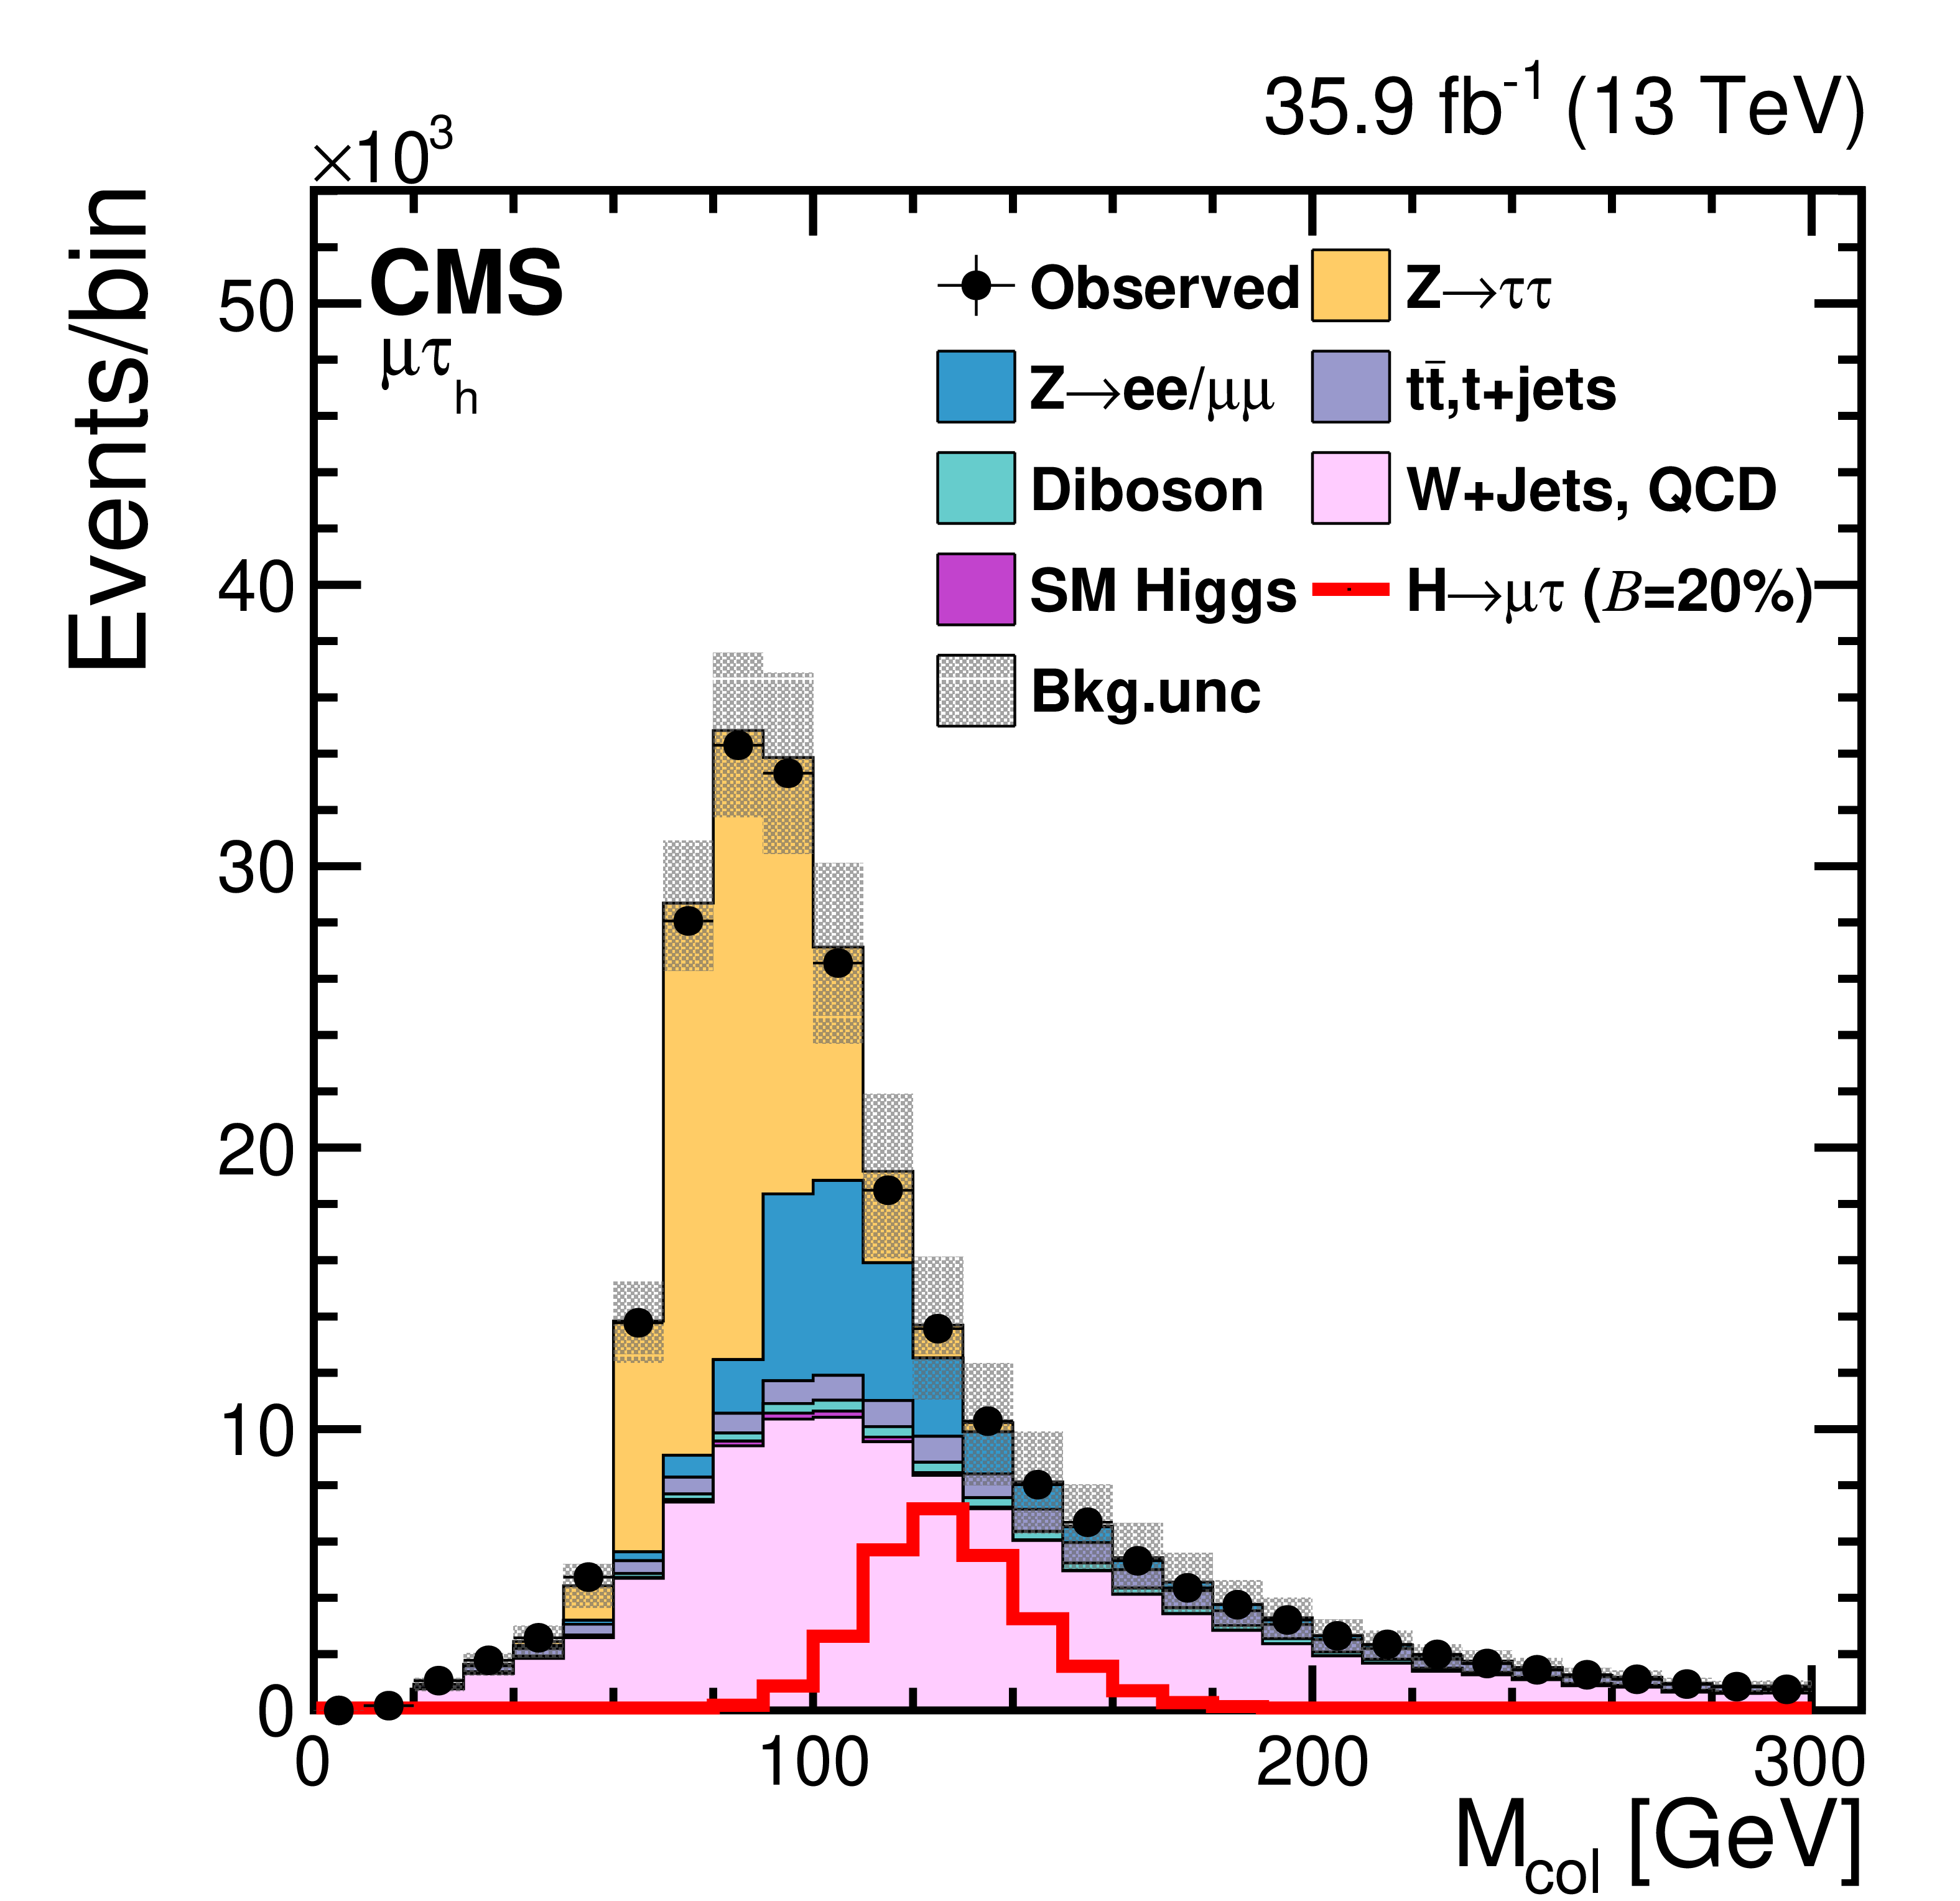
\includegraphics[width=0.49\textwidth]{plots/chapter5/CollMass2016.png}
  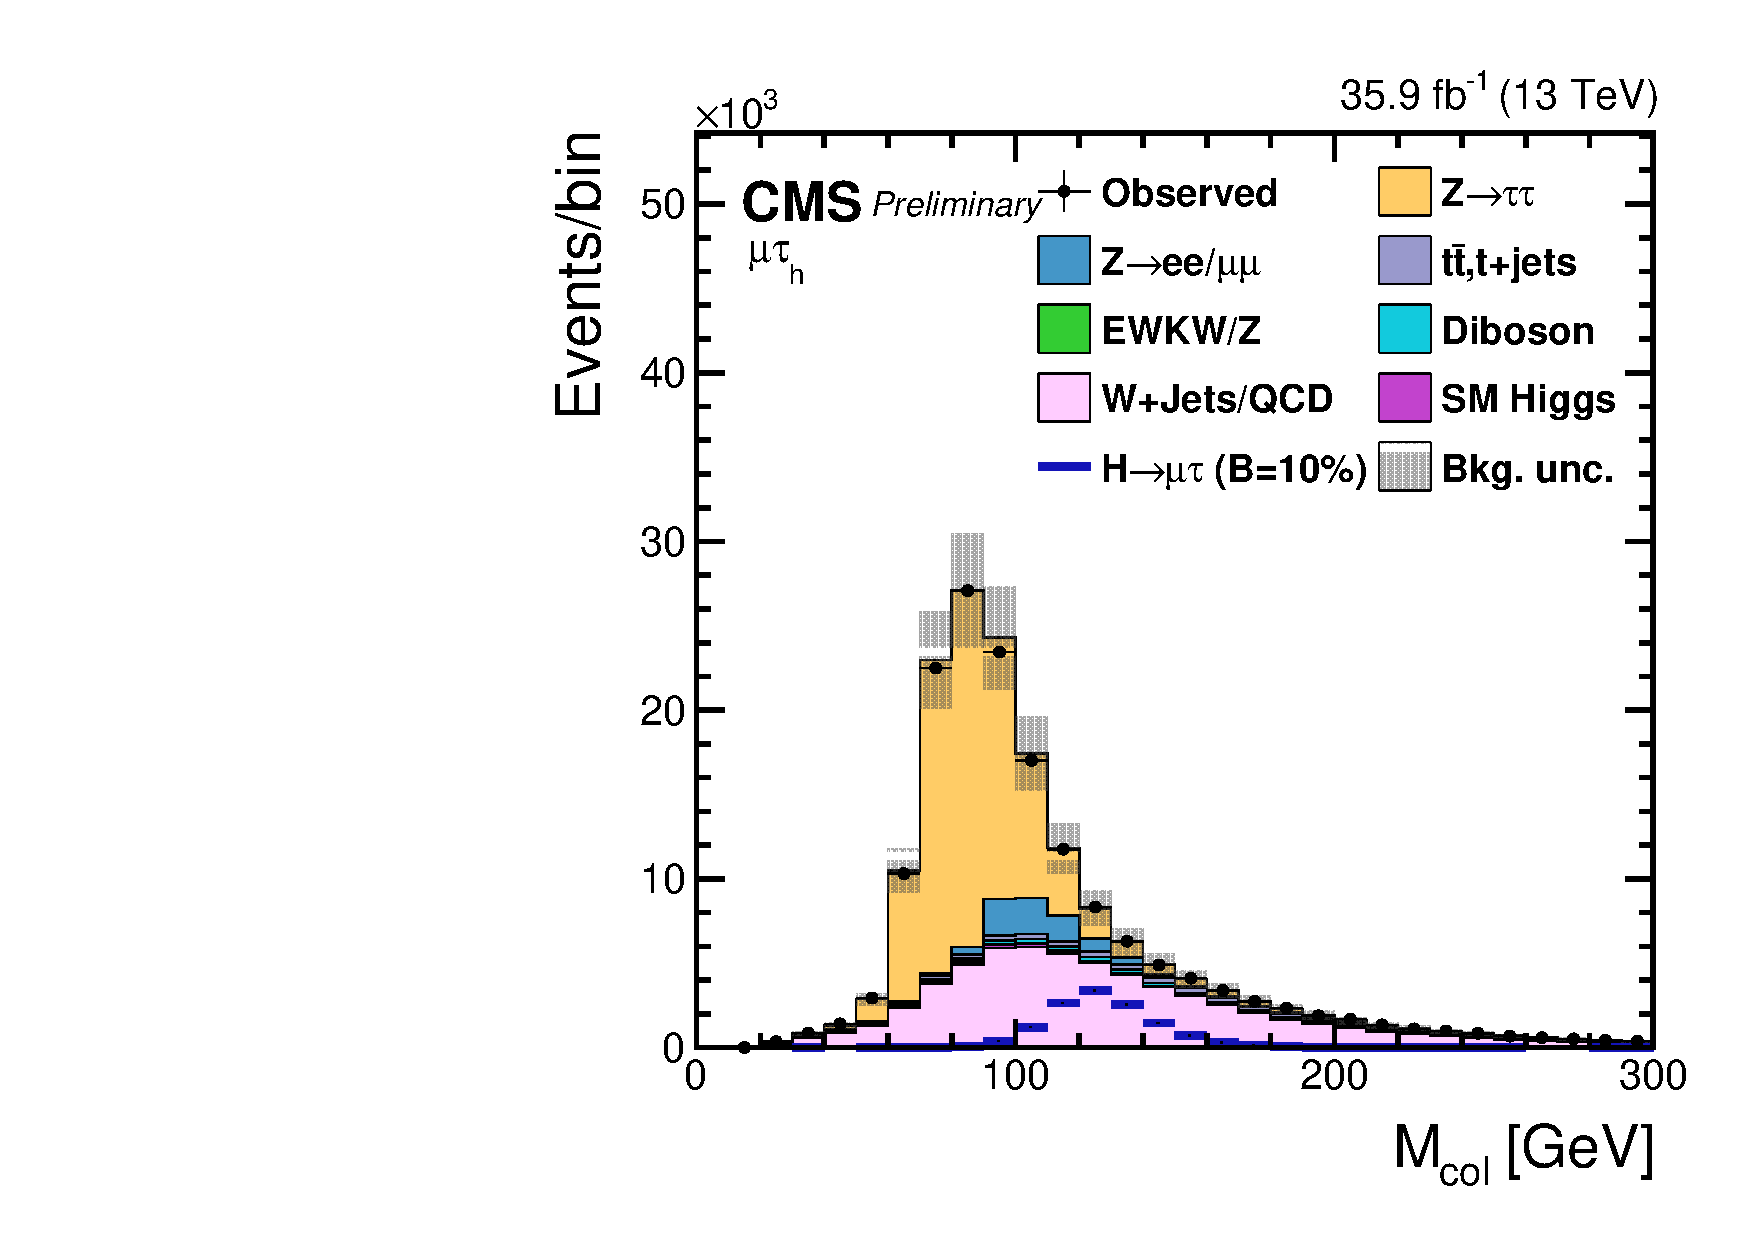
\includegraphics[width=0.49\textwidth]{plots/chapter5/CollMassRun2.pdf}
  \caption{Comparison of the collinear mass distribution from the previous analysis (left) compared to the current analysis (right). As can be seen from the plots, the \Zll($\ell=\Pe,\Pgm$) background and misidentified lepton background are significantly reduced in the current analysis. This can be attributed to using the DeepTau identification for hadronic taus.}
  \label{fig:collmass}
\end{figure}


\section{Jet reconstruction}

Quarks and gluons hadronize due to color confinement producing a fine spray of particles called jets~\cite{Cacciari:2008gp}. Jets are reconstructed using the anti-\kt clustering algorithm~\cite{Cacciari:2011ma}. This is a sequential clustering algorithm based on the quantities $d_{ij}$, which represents the distance between two entities, and $d_{iB}$, which represents the distance of the i-th object from the beam axis.

These distances are defined as:
\begin{equation}
  \begin{aligned}
  d_{ij}&= \text{min}(\text{k}_{\text{T}i}^{2p},\text{k}_{\text{T}j}^{2p})\frac{\Delta_{ij}^{2}}{\text{R}^2} \\
  d_{iB}&=\text{k}_{\text{T}i}^{2p}
  \end{aligned}
\end{equation}
where $\Delta_{ij}^{2}=(\eta_i-\eta_j)^2+(\phi_i-\phi_j)^2$, $\text{k}_{\text{T}i}$ is the transverse momentum of the i-th entity and R is the radius parameter which is set as 0.4.

In the anti-\kt clustering algorithm, $p=-1$, where the parameter $p$ governs the relative power of energy versus geometrical scales. The $d_{ij}$ represents the distance between all entity pairs present. If the minimum of those distances is smaller than the minimum distance $d_{iB}$ of any entity from the beam axis, those entities $i$ and $j$ are combined into a single entity. Otherwise, the object closest to the beam axis is considered a jet. It is then removed from the list of entities to be further clustered. The high \pt particles dominate in the anti-\kt and are clustered first. Softer constituents are subsequently clustered. Before the soft particles cluster among themselves, they cluster with hard particles. As a result of this, a hard particle with no hard neighbors within a distance 2R accumulates all the soft particles within a circle of radius R. Anti-\kt tries to produce jets with somewhat conical shapes which are centered around the hardest particles of the event. The boundaries are resilient to the effect of infrared and collinear radiation.

The reconstructed jets' energy differs from their true values as they are complex objects suffering from several effects. Correction factors are applied to calibrate their \pt and ensure a uniform response in $\eta$~\cite{Chatrchyan:2011ds, Khachatryan:2016kdb}. The energy coming from the pileup that has been clustered into the jet needs to be corrected. This is corrected using the hybrid jet area method. This method is a combination of the average offset method and the jet area method. The average amount of energy added to the event due to pileup is measured using the zero bias events in the average offset method. This relies on the assumption that averaging over zero bias events makes this measurement insensitive to high \pt objects. The average offset is measured in bins of $\eta$, and the number of pileup vertices (\npv) averaged over $\phi$. The correction is then given by $1-\frac{<\text{Offset}(\npv,\eta)>}{\pt^{\text{RAW}}}$, where $\pt^{\text{RAW}}$ is the uncorrected jet \pt. The other assumption is that every jet contains the same amount of pileup contribution, which is a drawback for this method.

The jet area method calculates corrections on a jet-by-jet basis. The energy density per event is calculated by clustering jets using the \kt algorithm. The \kt algorithm favors clustering soft jets as opposed to hard ones. The \pt is then divided by jet area, which is defined as the region in $\eta$--$\phi$ occupied by soft particles clustered in the jet. The median of this distribution ($\rho$) for an event is expected to be insensitive to hard particles. This $\rho A_{i}$ is a good approximation of pileup contribution to the i-th jet. However, this approach has a drawback because it doesn't consider the fact that the detector response is $\eta$ dependent. Thus, the hybrid jet area method combines these two methods to calculate a jet-by-jet correction depending on $\eta$ and \npv.

Jet momentum is determined as the vectorial sum of all particle momenta in the jet. It is found from simulation to be, on average, within 5 to 10\% of the true momentum over the whole \pt spectrum within detector acceptance~\cite{CMS:2017wyc}. Data collected in the ECAL endcaps were affected by noise during the 2017 run. This effect is mitigated by discarding events with jets having $\pt < 50 \GeV$ and $2.65 < \aeta < 3.139$ in 2017 dataset. Hadronic jets that contain b quarks are tagged using a DNN called the DeepCSV algorithm, and we use a WP with efficiency $\approx 70\%$~\cite{Sirunyan:2017ezt}.

The energy of reconstructed jets is corrected with an MC calibration factor to match the generated MC particle jet energy on average. The energy response of reconstructed jets is calibrated to be uniform with respect to $\eta$ and \pt. A QCD dijet sample is used to correct the dependence on $\eta$. Using jets that are approximately back-to-back in the azimuthal direction but at different $\eta$ regions of the detector, the difference in response between these two $\eta$ regions can be ascertained and corrected. Using the same method of measuring residual response in the transverse direction in \gjets or \zjets events, the absolute jet energy scale as a function of \pt can be made uniform~\cite{Khachatryan:2016kdb}. Additional selection criteria are applied to each jet to remove jets potentially dominated by instrumental effects or reconstruction failures. When combining information from the entire detector, the jet energy resolution amounts typically to 15\% at 10~\GeV, 8\% at 100~\GeV, and 4\% at 1~\TeV. Any jet within $\Delta\text{R}=0.5$ of the identified leptons is removed.


\section{Missing transverse energy}

Neutrinos and other hypothetical particles that are weakly interacting cannot be detected in the CMS detector. The momentum imbalance in the transverse plane can be used to infer their presence. The missing transverse momentum vector \ptvecmiss is computed as the negative vector sum of all the PF candidates' transverse momenta in an event $\ptvecmiss = -\Sigma\ptvec$, and its magnitude is denoted as \ptmiss~\cite{Sirunyan:2019kia}. The \ptvecmiss is modified to account for corrections to the reconstructed jets' energy scale in the event. Anomalous high-\ptmiss events can be due to various reconstruction failures, detector malfunctions, or non-collision backgrounds. Such events are rejected by event filters designed to identify more than 85--90\% of the spurious high-\ptmiss events with a mistagging rate less than 0.1\%~\cite{Sirunyan:2019kia}. In addition to the event filtering algorithms, the jet identification selection imposed, which requires the neutral hadron energy fraction of a jet to be less than 0.9, rejects more than 99\% of the noisy jets, independent of jet \pt, with a negligible mistag rate.

Corrections to the \ptvecmiss are applied to reduce the mismodeling of the simulated \PZ, \PW, and Higgs boson samples. The corrections are applied to the simulated events based on the vectorial difference of the measured missing transverse momentum and total transverse momentum of neutrinos originating from the decay of the \PZ, \PW, or Higgs boson. Their average effect is the reduction of the \ptmiss obtained from the simulation by a few \GeV. The \ptvecmiss plays a vital role in this analysis as it helps gauge the momentum of the neutrinos from the decaying tau lepton. The \ptvecmiss reconstruction is directly dependent on the reconstruction of all the other objects in the event, from jets to muons to electrons. Consequently, it is sensitive to all the effects that influence these objects' precise reconstruction and calibration.


\section{Relative isolation}
\label{isolation}
The muon (electron) isolation is measured relative to its $\pt^\ell (\ell=\Pe,\Pgm)$, by summing over the \pt of PF particles in a cone with $\text{R}=0.4(0.3)$ around the lepton:
\begin{linenomath*}
  \begin{equation*}
    I^\ell_{\text{rel}} = \left( \sum \pt^{\text{PV\;charged}} + \text{max}\left[0, \sum \pt^{\text{neutral}} + \sum \pt^\Pgg - \pt^{\text{PU}}(\ell)\right]\right) \biggm/ \pt^\ell,
  \end{equation*}
\end{linenomath*}
where $\pt^{\text{PV\;charged}}$, $\pt^\text{neutral}$, and $\pt^{\Pgg}$ indicate the \pt of a charged particle, a neutral particle, and a photon within the cone, respectively. The neutral contribution to isolation from pileup, $\pt^\text{PU}(\ell)$, is estimated from the area of the jet and the median energy density of the event~\cite{Cacciari:2008gn, Cacciari:2007fd} for the electron or from the sum of transverse momenta of charged hadrons not originating from the PV scaled by a factor of 0.5 for the muons. The charged contribution to isolation from the pileup is rejected by requiring the tracks to originate from the PV.

%
% Chapter 6
%

\chapter{Event Selection}
\label{evt_sel}

\section{Introduction}
\label{evt_sel_intro}
This chapter summarizes the event selection criteria for the analysis. The signal topology consists of an isolated lepton, \Pgm\, or \Pe, along with an oppositely charged isolated tau lepton (\taum, \taue, or \tauh). Jets misidentified as electrons or muons are suppressed by imposing isolation requirements. The events are first categorized into \mutau and \etau and then further divided into leptonic and hadronic channels based on tau decay mode. Figure ~\ref{fig:feynman} shows the corresponding Feynman diagrams for the LFV \Hmt and \Het decays.

\begin{figure}[htbp]
  \centering
  \subfigure[]{ 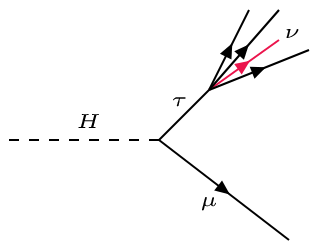
\includegraphics[width=0.3\textwidth]{plots/chapter6/Feynman/Hmuhad.png} }
  \subfigure[]{ 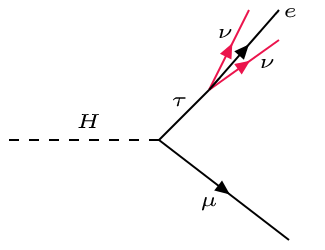
\includegraphics[width=0.3\textwidth]{plots/chapter6/Feynman/Hmue.png} } \\
  \subfigure[]{ 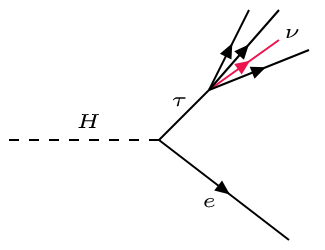
\includegraphics[width=0.3\textwidth]{plots/chapter6/Feynman/Hehad.png} }
  \subfigure[]{ 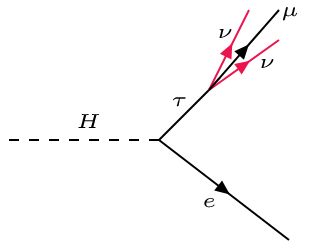
\includegraphics[width=0.3\textwidth]{plots/chapter6/Feynman/Hemu.png} } \\
  \caption{Feynman diagrams of lepton-flavor violating Higgs-boson decays. The first row shows diagrams for the Higgs boson coupling to \mutau (a,b). Couplings to \etau (c,d) are shown in the second row. Taus can decay leptonically or hadronically. Feynman diagrams are shown for the leptonic decay of taus (b,d) and the hadronic decay of taus (a,c).}
  \label{fig:feynman}
\end{figure}

The final states of this analysis are similar to the \Htt decay allowed by the SM and since been observed ~\cite{Sirunyan:2017khh}. However, there are some significant kinematic differences. The LFV \Hmuhad and \Hmue (\Hehad and \Hemu) decays consist of a muon (an electron) that comes directly from the Higgs and has a hard \pt spectrum, along with a hadronically decaying tau or a softer electron (muon) that comes from the tau lepton of opposite sign charge, and missing transverse momentum from the tau decay. Also, there are fewer neutrinos in LFV decays, coming from the decay of the single \Pgt. The decay products of this highly boosted tau are closely aligned, leading to a narrow separation between the visible decay products of the tau and the \ptvecmiss in the azimuthal plane. The same is not true in the \Htt decays. These differences are illustrated pictorially in Figures ~\ref{fig:htt_v_lfv_mt} and ~\ref{fig:htt_v_lfv_et}.

\begin{figure}[htbp]
  \centering
  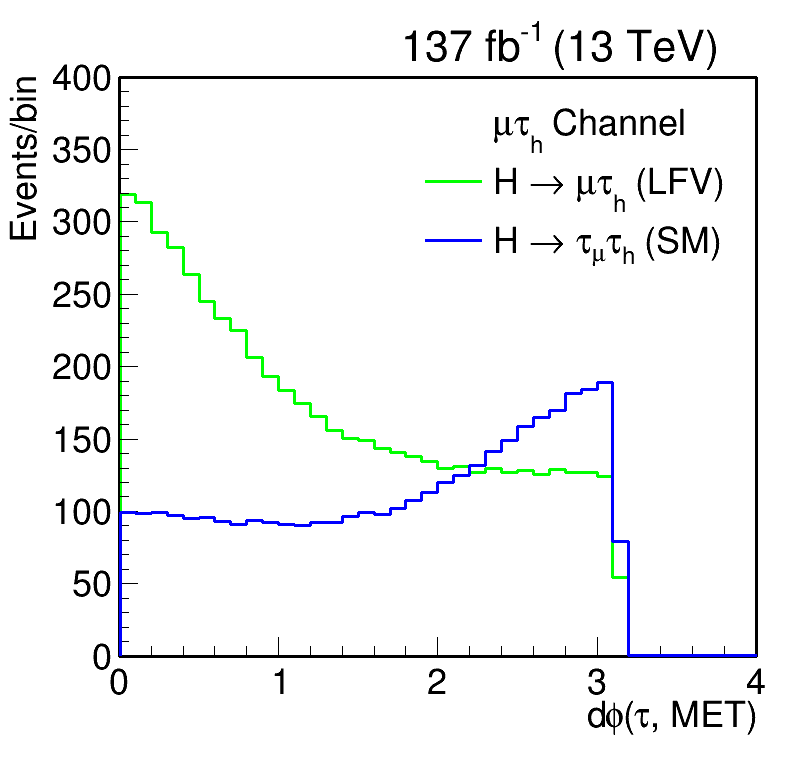
\includegraphics[width=0.45\textwidth]{plots/chapter6/LFVvSM/MTdphi.png}
  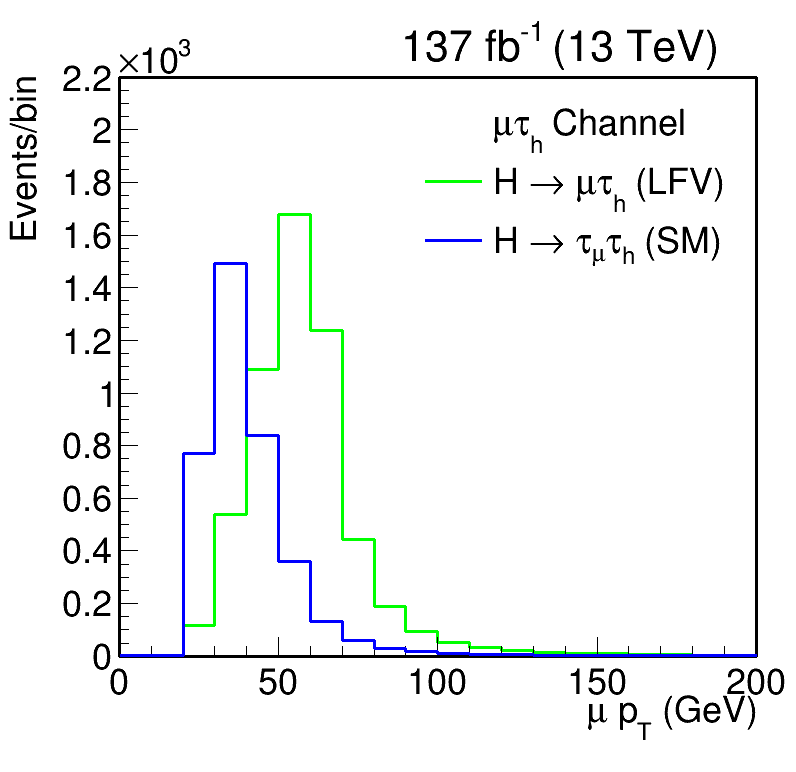
\includegraphics[width=0.45\textwidth]{plots/chapter6/LFVvSM/MTmpt.png} \\
  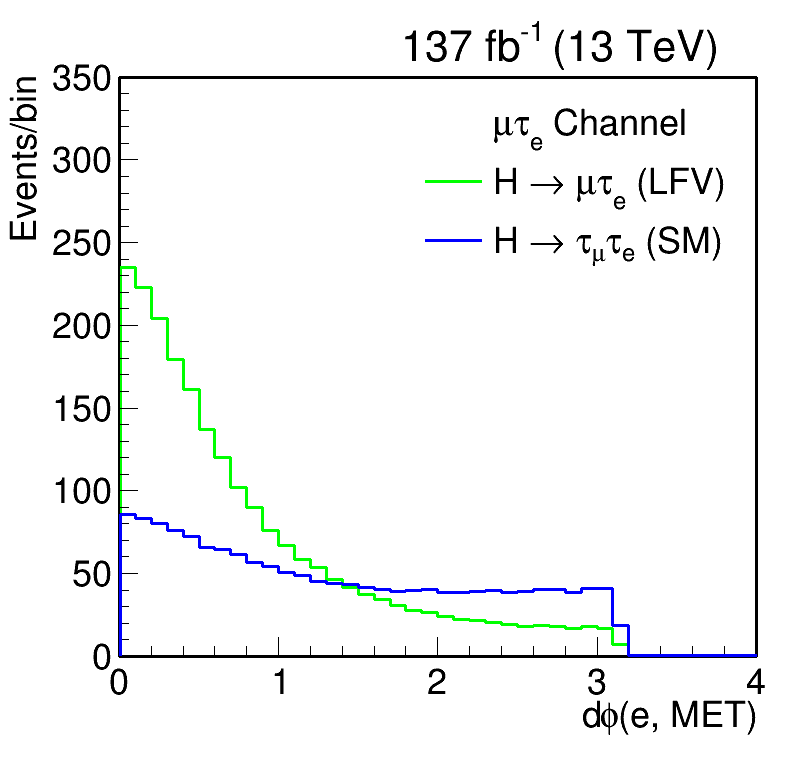
\includegraphics[width=0.45\textwidth]{plots/chapter6/LFVvSM/MEdphi.png}
  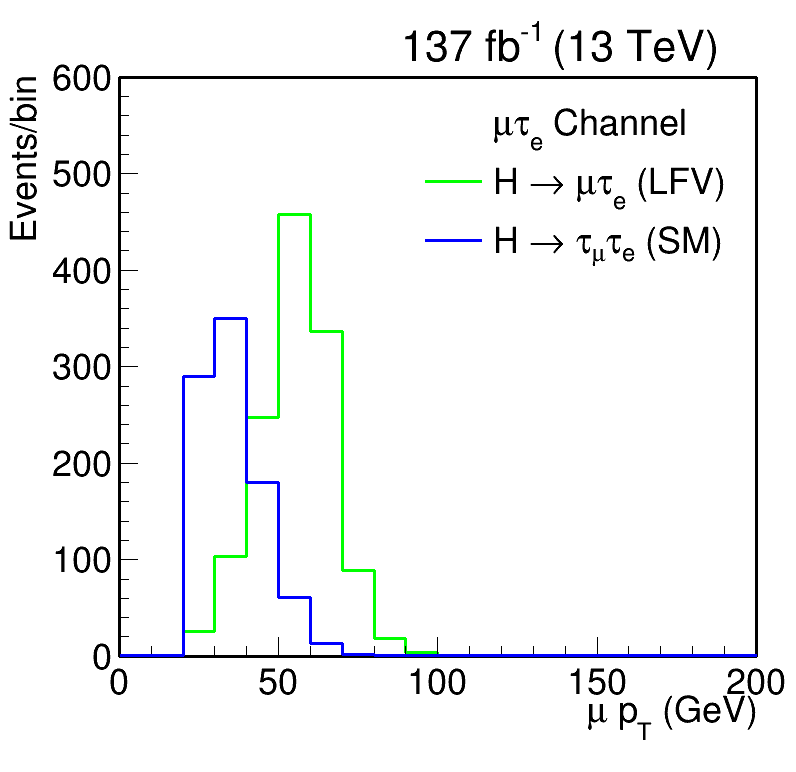
\includegraphics[width=0.45\textwidth]{plots/chapter6/LFVvSM/MEmpt.png} \\
  \caption{Illustration of the differences in $d\phi(\ell = \Pgt \; or \; \Pe, MET)$ and $\pt^{\Pgm}$ spectrums in LFV and SM \Htt processes.}
  \label{fig:htt_v_lfv_mt}
\end{figure}

\begin{figure}[htbp]
  \centering
  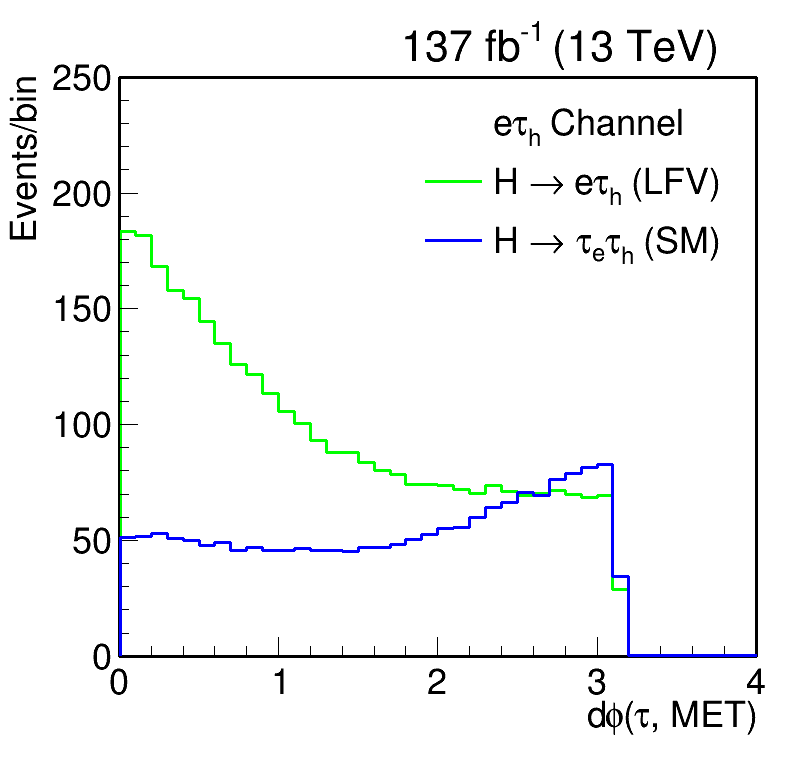
\includegraphics[width=0.45\textwidth]{plots/chapter6/LFVvSM/ETdphi.png}
  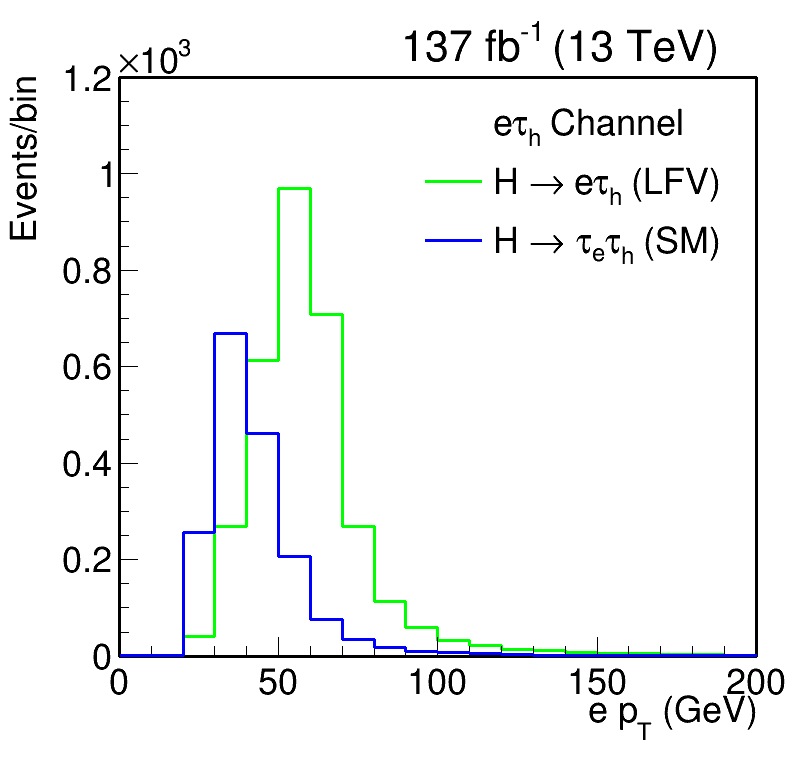
\includegraphics[width=0.45\textwidth]{plots/chapter6/LFVvSM/ETept.png} \\
  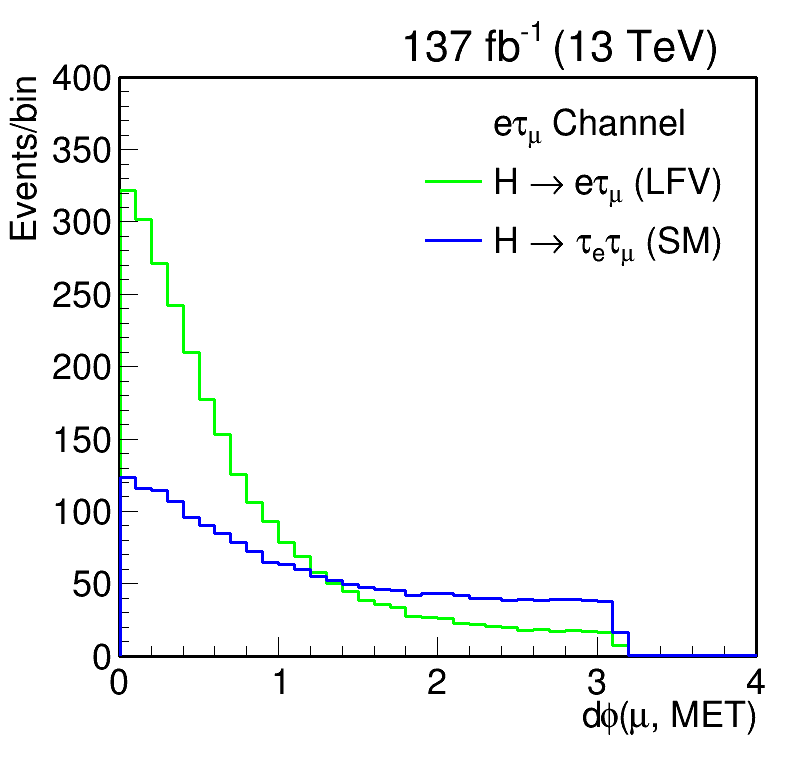
\includegraphics[width=0.45\textwidth]{plots/chapter6/LFVvSM/EMdphi.png}
  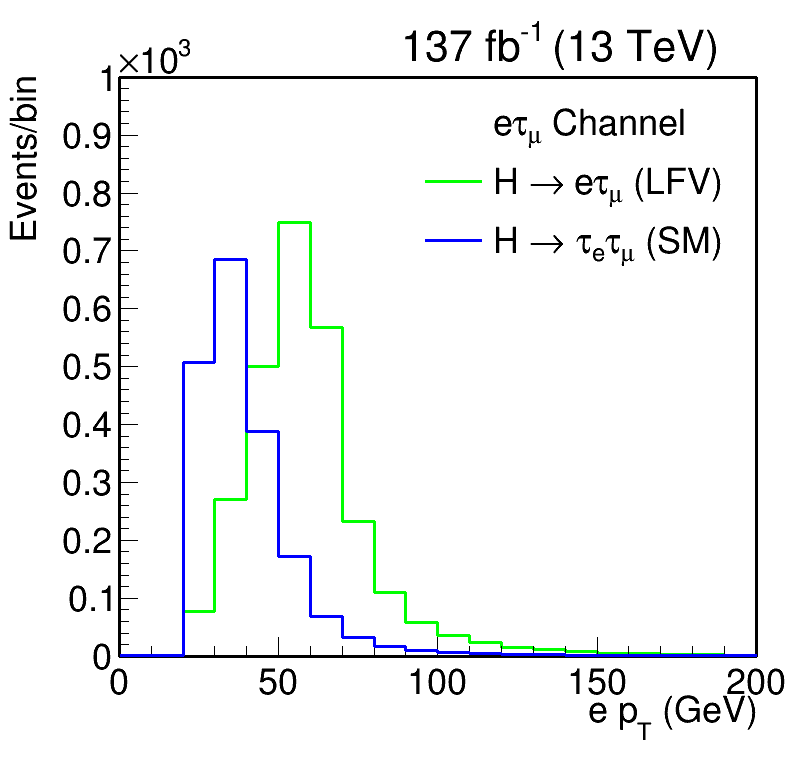
\includegraphics[width=0.45\textwidth]{plots/chapter6/LFVvSM/EMept.png} \\
  \caption{Illustration of the differences in $d\phi(\ell = \Pgt \; or \; \Pgm, MET)$ and $\pt^{\Pe}$ spectrums in LFV and SM \Htt processes.}
  \label{fig:htt_v_lfv_et}
\end{figure}

In each decay mode (\Hemu, \Hehad, \Hmue, \Hmuhad), a set of loose selection (preselection) for the respective signature is first defined. The jets in the event are required to have a $\pt > 30\GeV$ and $\abs{\eta} < 4.7$. The event in each decay channel is divided into categories based on the number of jets in the event (0-jet, 1-jet, 2-jet) to enhance the contribution of different Higgs boson production mechanisms.

The 0-jet category enhances the Gluon Gluon Fusion (GGF) Higgs production contribution, while the 1-jet category enhances the GGF Higgs production with initial-state radiation. The 2-jet category is further broken into two based on the invariant mass of the two jets (\mjj). The threshold of 550 (500)\GeV on \mjj for \mutau(\etau) channels has been optimized to give the best-expected exclusion limits. Events with $\mjj < 550(500)\GeV$ enhances GGF Higgs production contribution while $\mjj \ge 550(500)\GeV$ enhances VBF Higgs production contribution.

To better discriminate between signal and background events, a Boosted Decision Trees (BDT) discriminator is trained using simulated events, using the TMVA tool of the ROOT analysis package ~\cite{Hocker:2007ht}. After applying preselection, a binned likelihood is used to fit the distribution of a BDT discriminator for the signal and the background contributions, and we call this the BDT fit method. The collinear mass (\mcol) and the transverse mass ($\mt(\ell)$) that are used as input variables to the BDT are defined in the following paragraphs. A brief description of the BDT is given in the next section.

The \mcol provides an estimate of \mh using the observed decay products of the Higgs boson candidate. It is reconstructed using the collinear approximation based on the observation that, since $\mh \gg m_\Pgt$, the \Pgt\, lepton decay products are highly Lorentz boosted in the direction of the \Pgt\, candidate ~\cite{Ellis:1987xu}. The momentum of the neutrino coming from \Pgt\, decay can be approximated to have the same direction as the visible decay products of the \Pgt(\vectvis). Figure ~\ref{fig:METproj} shows the corresponding Feynman diagram for the \met projected in the direction of the visible decay products of tau.

\begin{figure}[htbp]
  \centering
  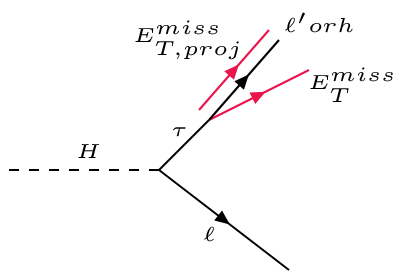
\includegraphics[width=0.49\textwidth]{plots/chapter6/Feynman/METproj.png}
  \caption{Estimation of the neutrino momentum \metproj by using the component of the missing transverse energy \met which is collinear to the visible decay products of tau in the transverse plane.}
  \label{fig:METproj}
\end{figure}

The component of the \ptvecmiss in the direction of the visible \Pgt\, lepton decay products, is used to estimate the transverse component of the neutrino momentum (\ptnu). The collinear mass can then be derived from the visible mass of the $\Pgm-\Pgt$ or $\Pe-\Pgt$ system (\mvis) as $\mcol = \mvis/\sqrt{x_\tvis}$, where $x_\tvis$ is the fraction of energy carried by the visible decay products of the \Pgt ($x_\tvis = \ptvis/(\ptvis + \ptnu)$), and \mvis is the invariant mass of the visible decay products.

The $\mt(\ell)$ is a variable constructed from the lepton momentum and the missing transverse momentum vectors: $\mt(\ell) = \sqrt{2\abs{\vec{p}_{\text{T}}^\ell}\abs{\ptvecmiss} (1-\text{cos}\Delta\phi_{\ell-\ptvecmiss})}$, where $\Delta\phi_{\ell-\ptvecmiss}$ is the angle in the transverse plane between the lepton and the missing transverse momentum, which is used to discriminate the Higgs boson signal candidates from the \wjets background.

An alternate analysis has been implemented to cross-check the results obtained from the BDT fit method. This approach involves placing requirements on several kinematic variables and then using the resulting distribution of \mcol as a discriminant for a binned likelihood fit. Henceforth, we call this the \mcol fit method. The BDT and \mcol fit methods were performed blinded in the signal region ~\cite{Roodman:2003rw}. The selection criterion described was developed without looking at the data in the region where the signal is expected. This approach is standard in particle physics analysis and eliminates the experimenter’s bias. We use a blinding criteria of $\frac{s}{\sqrt{s+b}} > 0.2$ for the plots that are shown in this chapter.

\section{Boosted Decision Tree}
\label{bdt}
A decision tree is a tree structure in which there is a condition on an attribute at each internal node. Each branch represents the outcome of this condition, and each leaf node represents a class label. The tree structure is built based on binary splits Figure ~\ref{fig:dec_tree}. The starting point of the tree structure is called a root node containing all the events we want to classify. A sequence of binary splits is made using conditions on the input variables provided to the classifier. The variable which ensures the separation of the signal and the background is used for each split.

\begin{figure}[htbp]
  \centering
  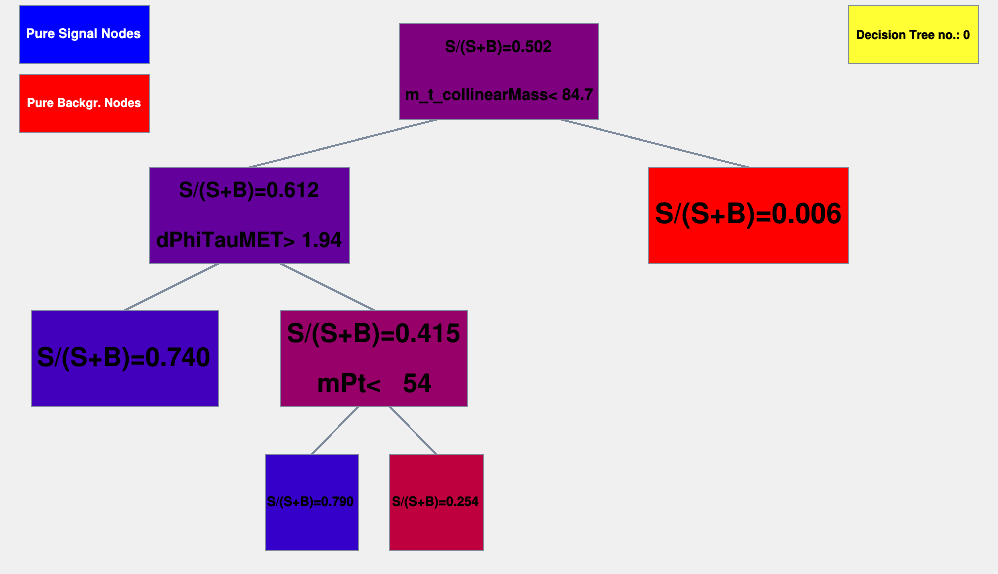
\includegraphics[width=0.8\textwidth]{plots/chapter6/BDT/BDT.png}
  \caption{Illustration of decision tree.}
  \label{fig:dec_tree}
\end{figure}

Gini Index is used as the separation criterion, and it is defined by $p.(1 - p)$, where p is the purity of the node. The purity of a node is given by the ratio of signal events to all events in that node. Since the splitting criterion is always a cut on a single variable, the training procedure selects the variable and cut value that optimizes the increase in the Gini Index between the parent node and the sum of the two daughter nodes' indices, weighted by their relative fraction of events. The same variable can thus be used for splitting several nodes, and the splitting is stopped when a predefined depth of the tree, purity of leaf nodes, the minimum number of events in a leaf node is reached. An event which ends up in a leaf node with a majority of signal events is classified as a signal event and vice versa.

A single decision tree is a weak classifier. The performance of weak classifiers can be enhanced using the Boosting technique. This technique works by building classifiers using reweighted training data and then taking a weighted majority vote of the sequence of classifiers thus produced. AdaBoost (adaptive boosting) method was used for boosting. AdaBoost is adaptive in that subsequent classifiers are tweaked in favor of those instances misclassified by previous classifiers. The misclassified event weights depend on the training error of each decision tree. The training error is calculated as

\begin{equation}
  \operatorname{err}_{m}=\frac{\sum_{i=1}^{N} w_{i} I\left(y_{i} \neq DT_{m}\left(x_{i}\right)\right)}{\sum_{i=1}^{N} w_{i}}
\end{equation}

in which the subscript m is the tree label and w is the event weight. The $y_{i}$ is the true label for the event, 1 for signal and -1 for background. $DT_{m}(x_{i})$ is the output of the decision tree. The variable $I(y_{i} \neq DT_{m}(x_{i}))$ equals 1 if $y_{i} \neq DT_{m}(x_{i})$ or 0 otherwise. The weight for event i is updated using $\alpha_{m}$ which is calculated from the training error. $\beta$ is the learning rate.

\begin{align}
  \alpha_{m}=\beta \times \ln \left(\left(1-\operatorname{err}_{m}\right) / \operatorname{err}_{m}\right) \\
  w_{i} \rightarrow w_{i} \times e^{\alpha I\left(y_{i} \neq DT_{m}\left(x_{i}\right)\right)}
\end{align}

By construction, the training error is $err_{m} \leq 0.5$ as the same training events used to classify the output nodes of the previous tree are used to calculate the training error. The learning rate parameter can be used to adjust the step size of each re-weighting. Event weights in each tree are renormalized to keep the summed weights constant. After the boosting and training processes, the final score of each event is $DT(x)$. A high score indicates a signal like event while a low score indicates a background like event.

\begin{equation}
DT(x)=\sum_{m=1}^{N_{tree}} \alpha_{m} DT_{m}(x)
\end{equation}

This technique also helps in stabilizing the response of the classifiers for fluctuations in the training data. It utilizes a predefined depth of the tree instead of pruning it to avoid overfitting to the training data. All the BDT trainings were done with an ensemble of 850 decision trees, with each tree having a maximum depth of 3. The minimum node size is required to be 2.5\%, and the learning rate is set to 0.5. A training to testing split of 50:50 was used.

\section{\texorpdfstring{\Hmuhad}{Hmutauh} channel}
The first step is to require the events to pass an isolated muon trigger. For 2016 data, this trigger has a muon \pt\, threshold of 24\GeV. However, for the 2017 and 2018 data, the trigger with a 24\GeV threshold is prescaled.  Prescaling corresponds to collecting one out of every n events to reduce the event rate. We use this trigger in conjunction with the isolated muon trigger with a muon \pt\, threshold of 27\GeV. In addition to the event passing the trigger, the reconstructed leptons corresponding to the trigger have to match the HLT objects within $\Delta R < 0.5$.

Next, the preselection begins by requiring an isolated \Pgm\, and an isolated \tauh candidates of opposite electric charge and separated by $\Delta\text{R} > 0.5$. The muon candidate is required to have $\pt > 26\GeV$, $\abs{\eta} < 2.1$ and isolation $I^{\Pgm}_\text{rel} < 0.15$. The \tauh candidate is required to have $\pt > 30\GeV$ and $\abs{\eta} < 2.3$. Events containing additional electrons, muons, or \tauh candidates are vetoed. Events with at least one b jet tagged by DeepCSV algorithm are rejected in order to suppress the \ttbar background.

A BDT is trained after applying preselection criteria. The signal training sample considered is a mixture of simulated GGF and VBF events, weighted according to their respective SM production cross-sections. The misidentified lepton background and \Ztt background are the dominant backgrounds in this channel. The background used for training the BDT is a data sample of misidentified lepton events with the same charge assignment for both leptons along with the Drell-Yan MC sample with signal selections. The input variables to the BDT are $\pt^{\Pgm}, \pt^{\tauh}$, \mcol, \ptvecmiss, \mt(\tauh, \ptvecmiss), \detamtauh, \dphimtauh, and \dphitauhmet. The distribution of the input variables to the BDT can be seen in Figure ~\ref{fig:input_mt}.

\begin{figure}[htbp!]
  \centering
  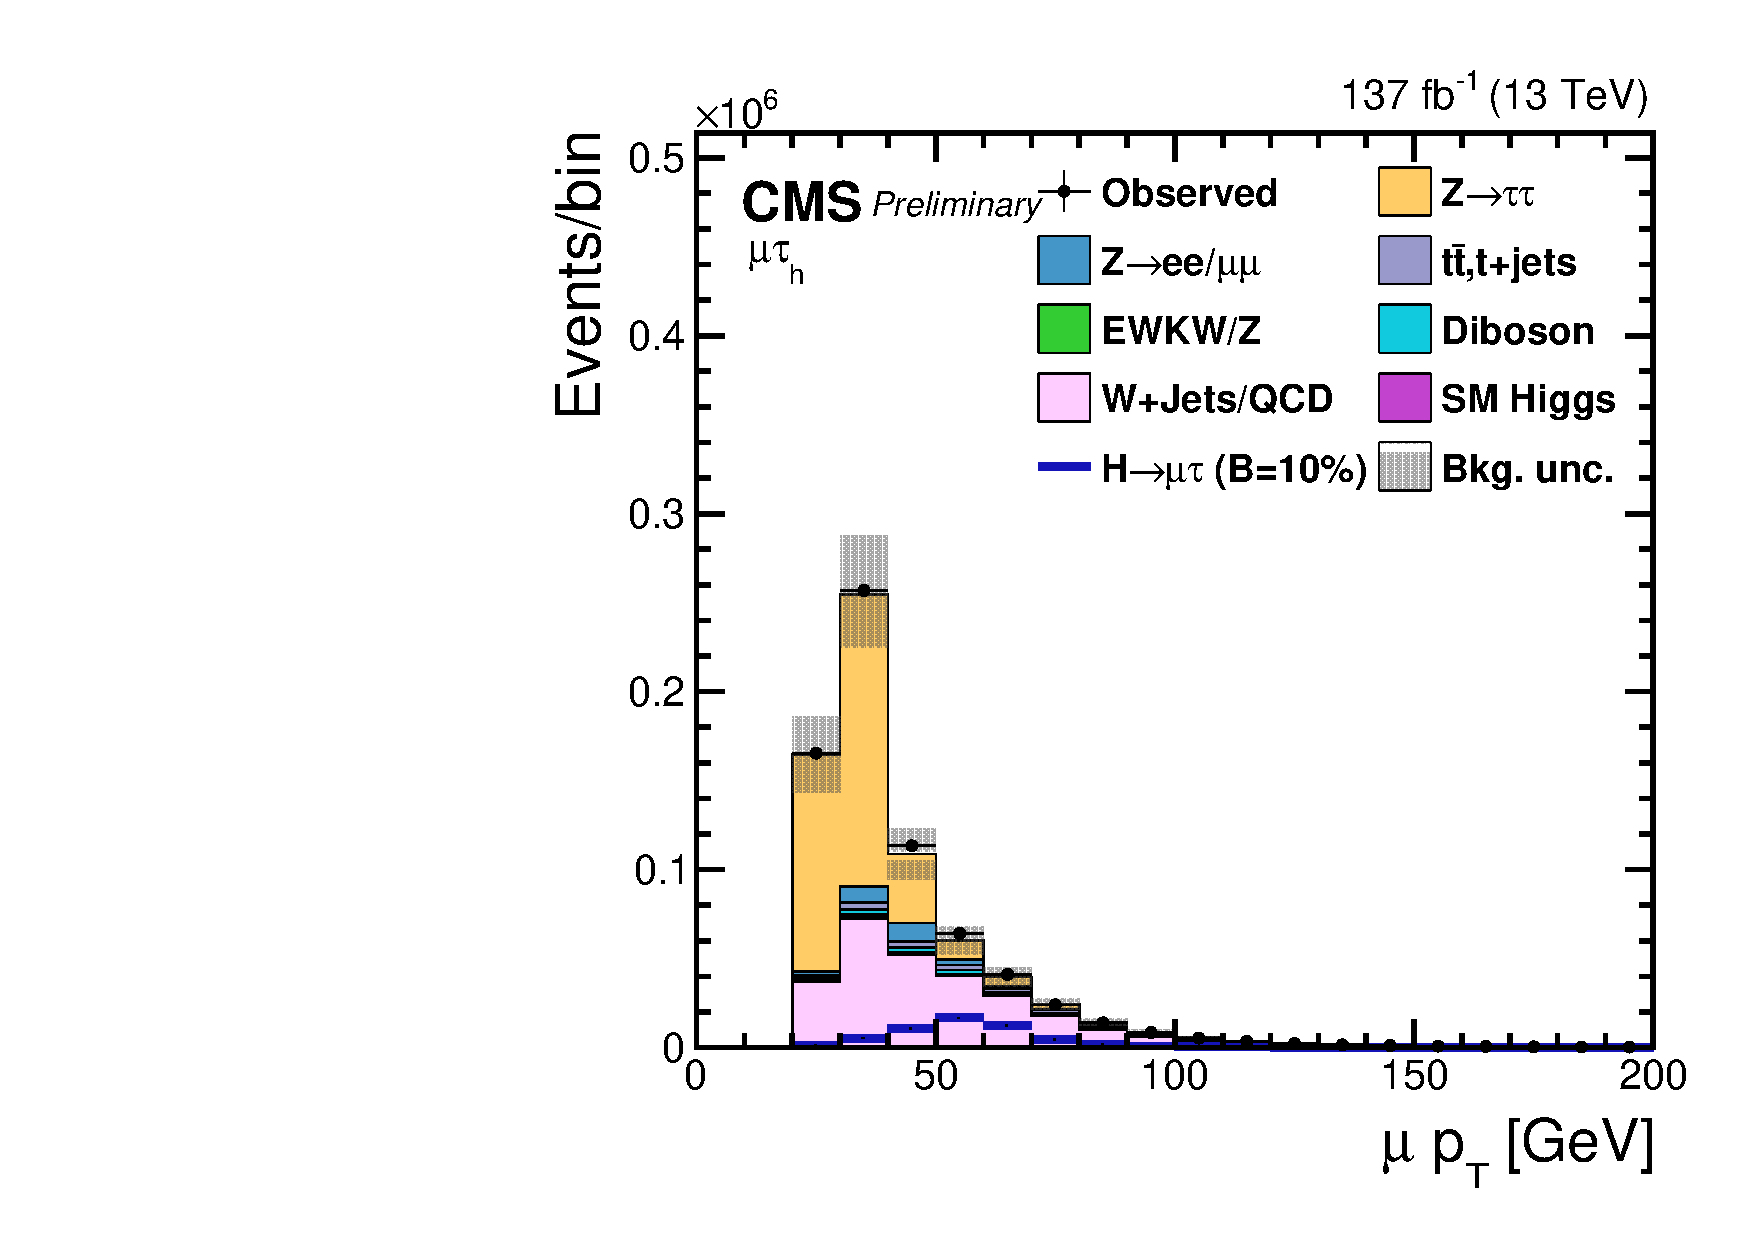
\includegraphics[width=0.36\textwidth]{plots/chapter6/mutau/mPt.pdf}
  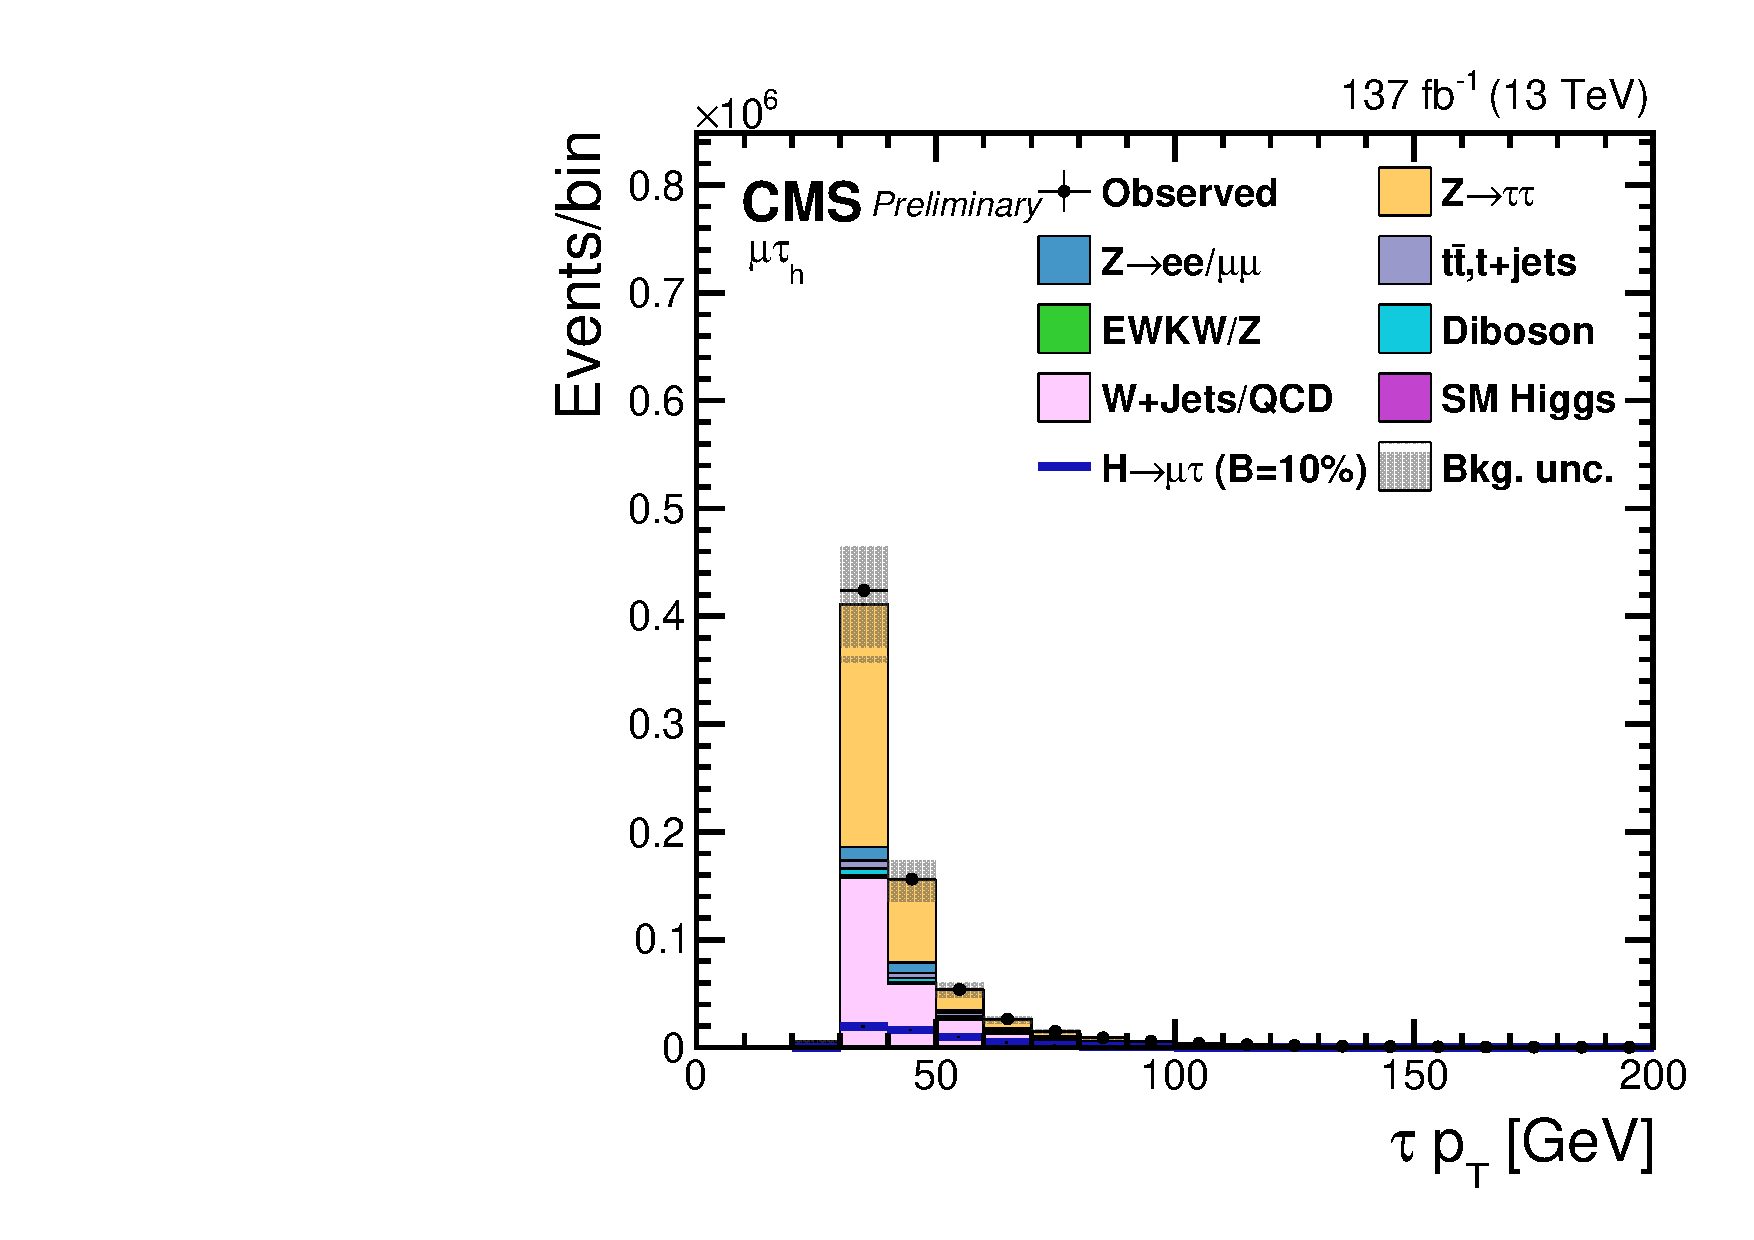
\includegraphics[width=0.36\textwidth]{plots/chapter6/mutau/tPt.pdf}\\
  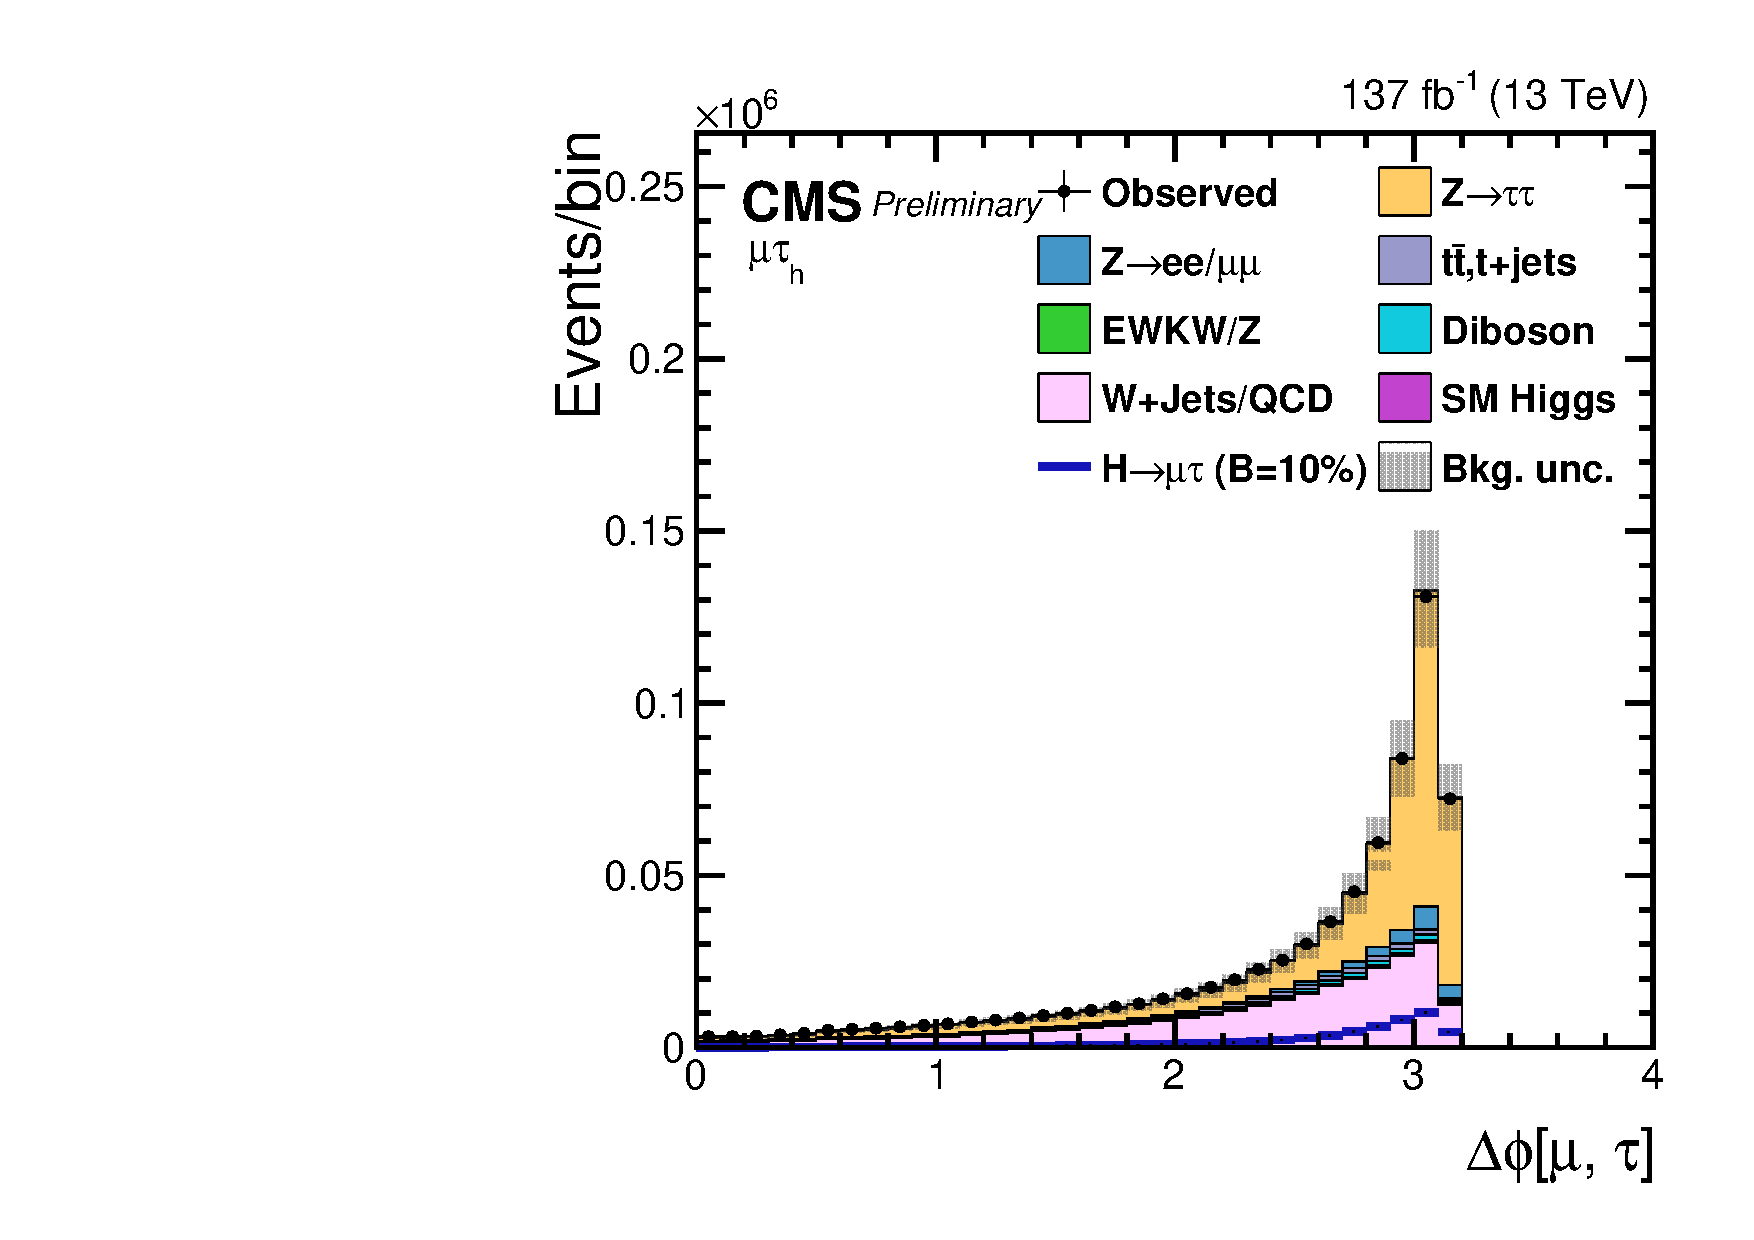
\includegraphics[width=0.36\textwidth]{plots/chapter6/mutau/dPhiMuTau.pdf}
  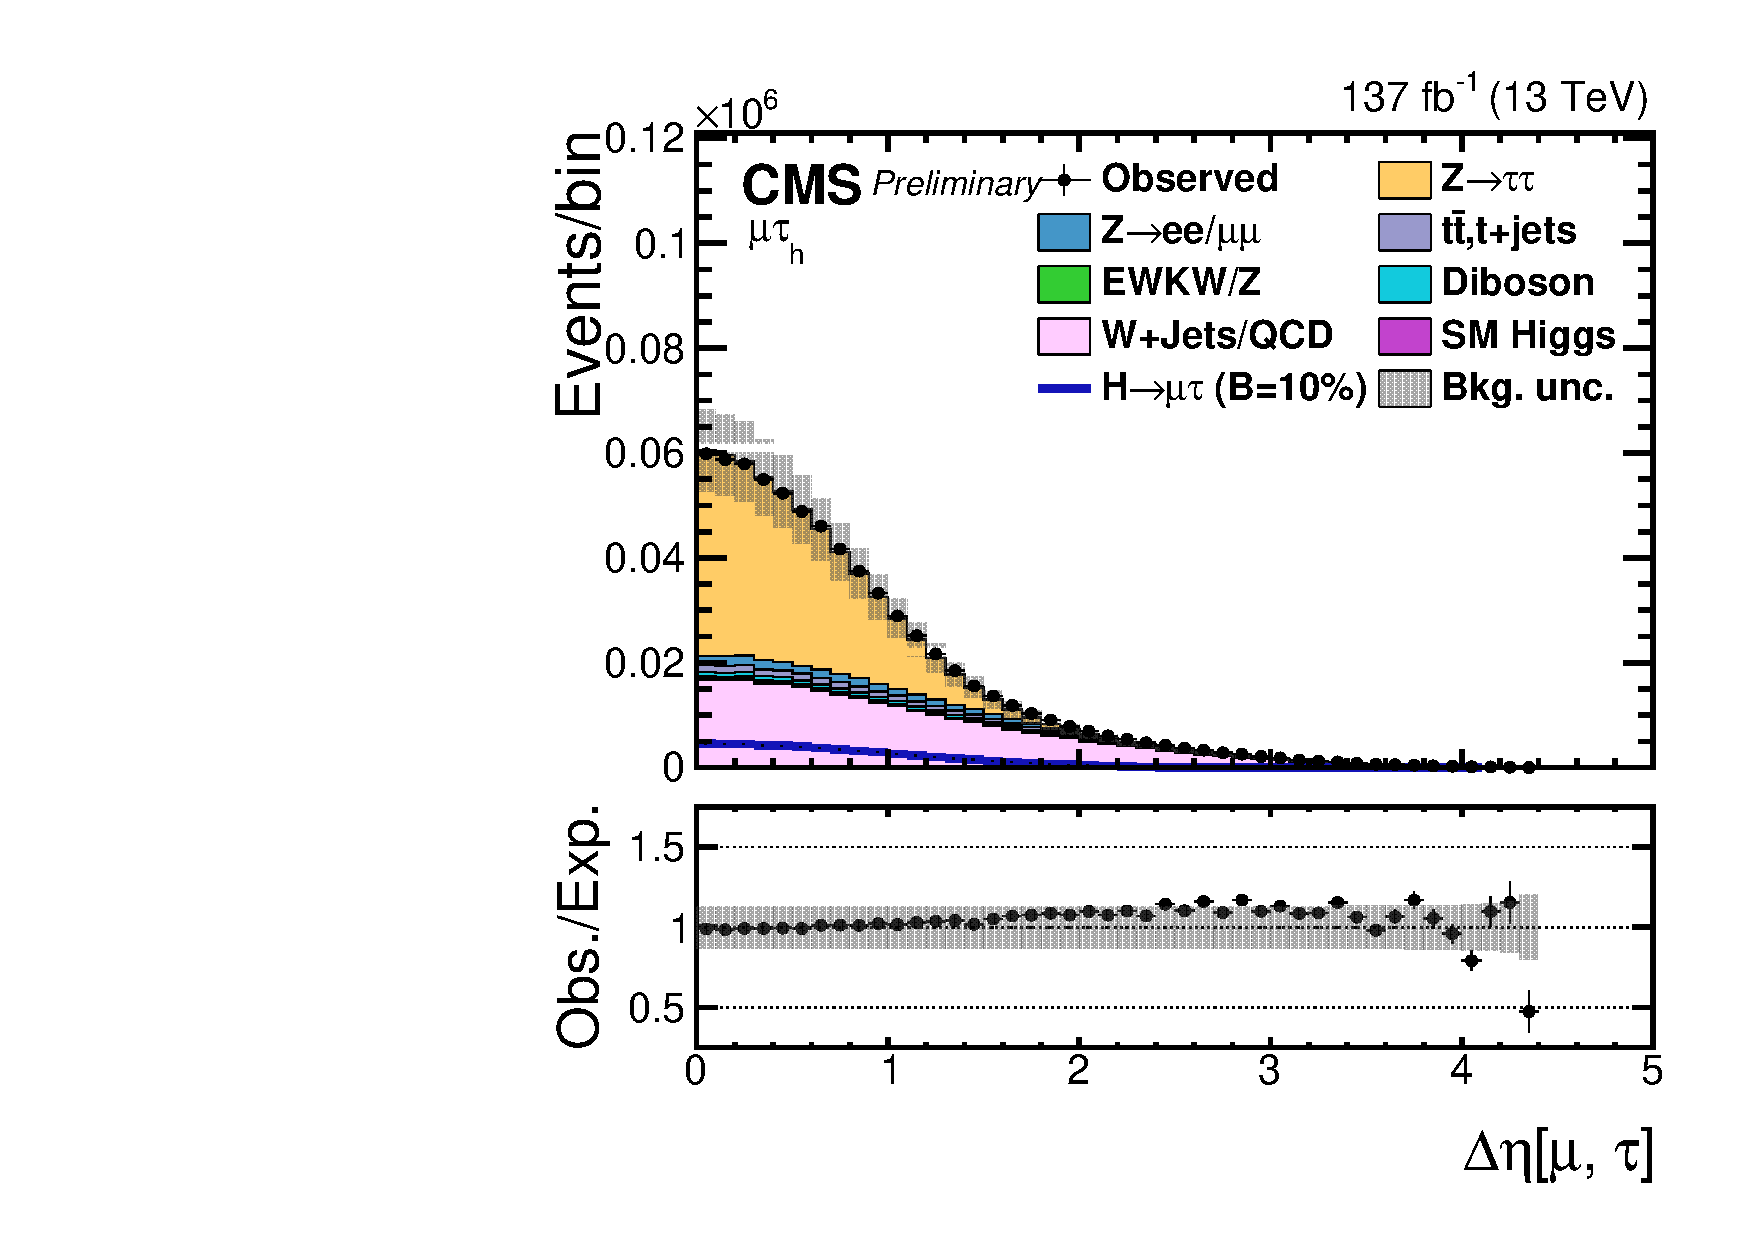
\includegraphics[width=0.36\textwidth]{plots/chapter6/mutau/dEtaMuTau.pdf}\\
  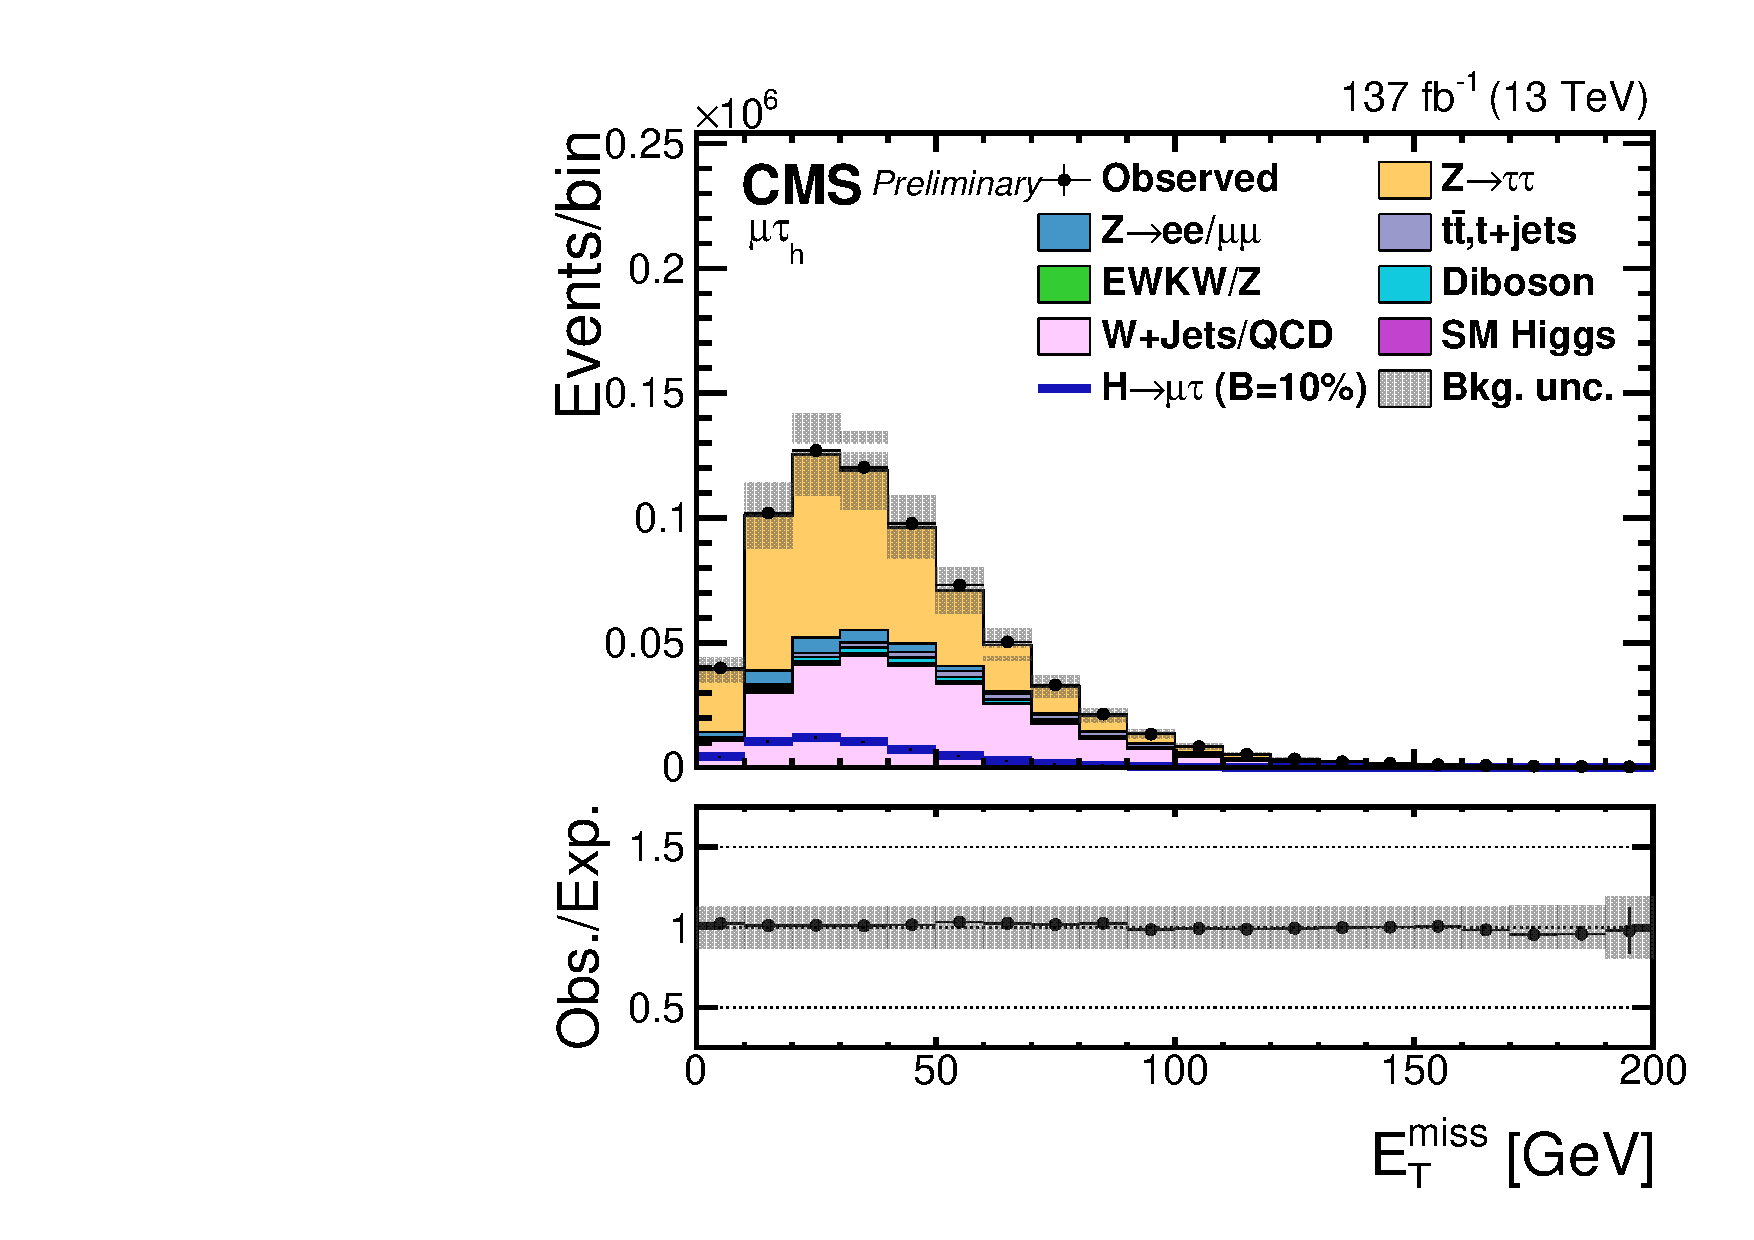
\includegraphics[width=0.36\textwidth]{plots/chapter6/mutau/type1_pfMetEt.pdf}
  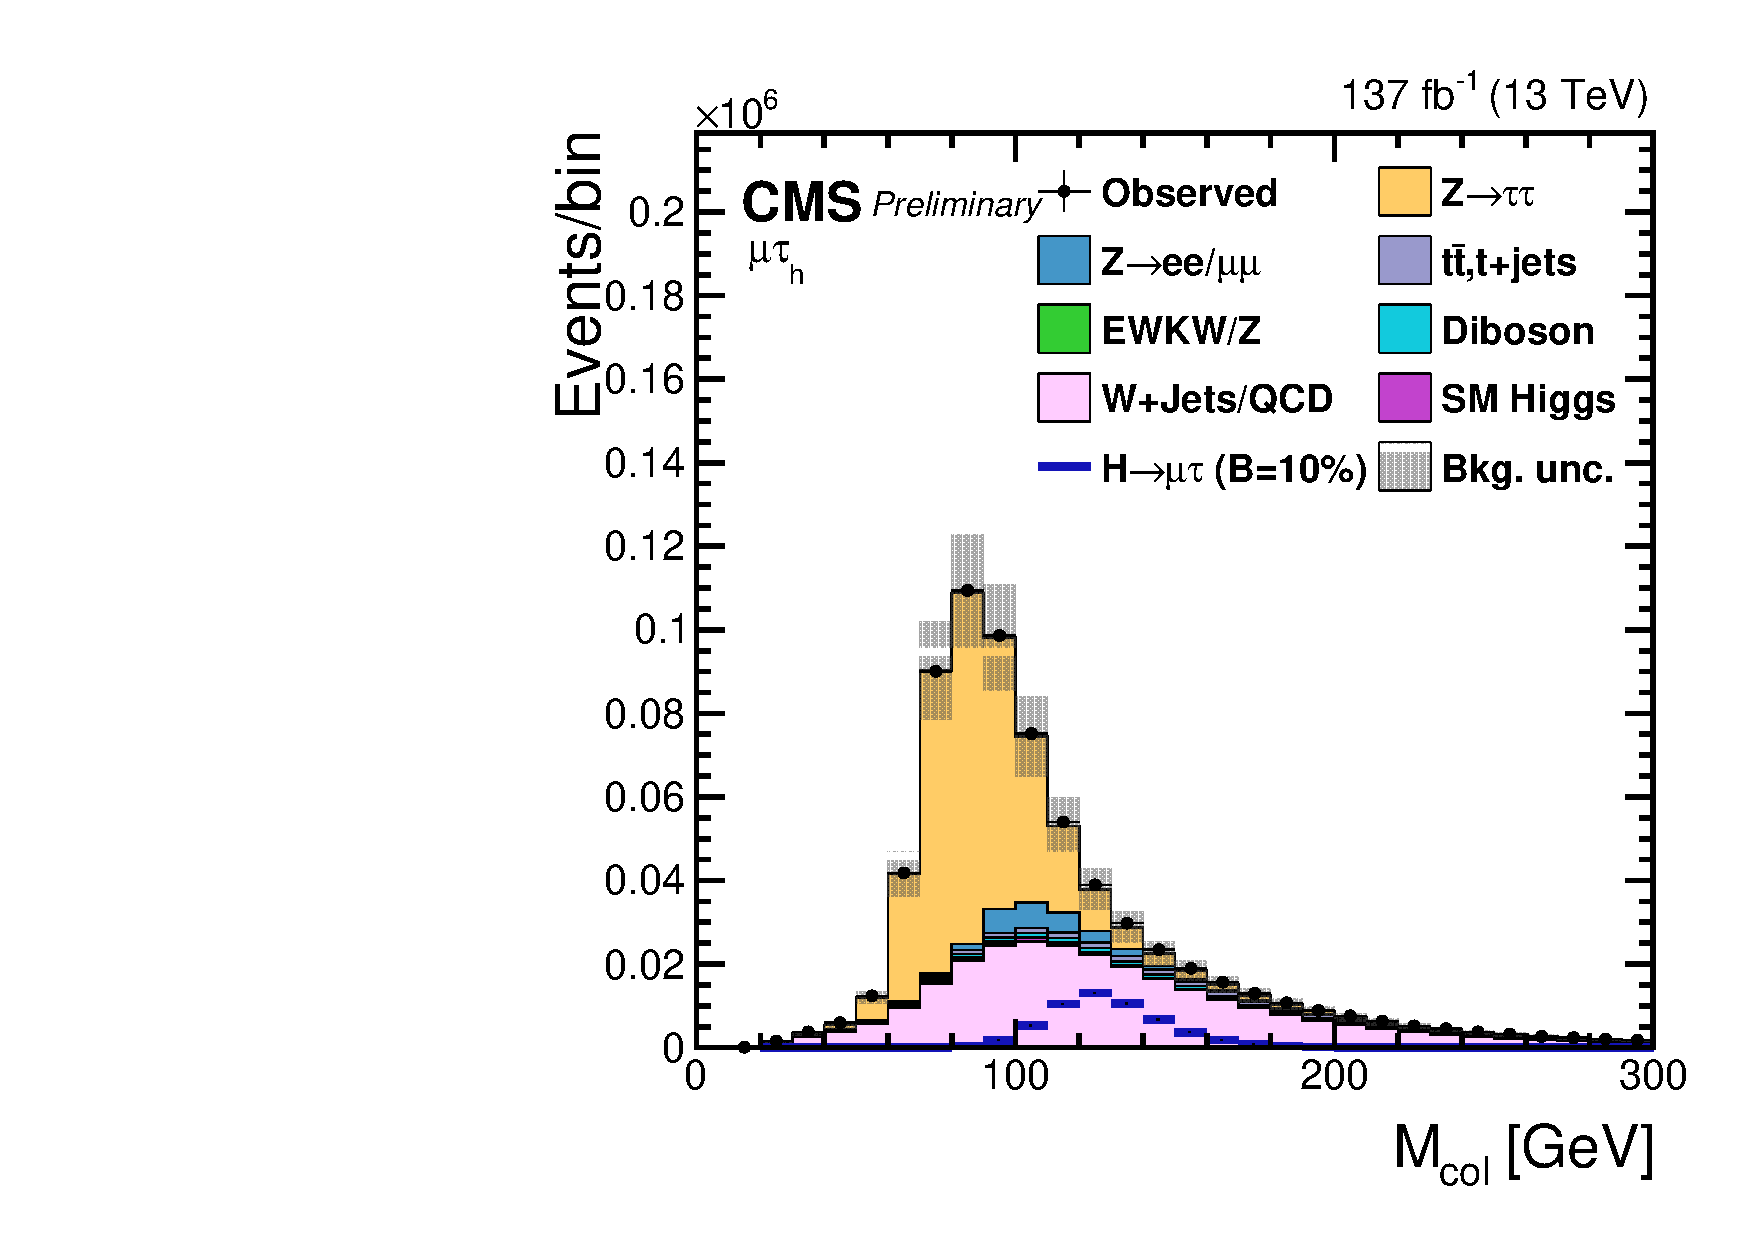
\includegraphics[width=0.36\textwidth]{plots/chapter6/mutau/m_t_CollinearMass.pdf}\\
  \includegraphics[width=0.36\textwidth]{plots/chapter6/mutau/MTTauMET.pdf}
  \includegraphics[width=0.36\textwidth]{plots/chapter6/mutau/dPhiTauMET.pdf}\\
  \caption{Distribution of the input variables to the BDT for the \Hmuhad process.}
  \label{fig:input_mt}
\end{figure}

The selection on \ptvecmiss is motivated by the presence of neutrinos in the \Pgt\, lepton decays. The neutrino is expected to be collinear with \tauh, which leads to selection on the \dphitauhmet variable. The two leptons are usually in the opposite direction in the azimuthal plane, which leads to selection on the \dphimtauh variable. The BDT discriminator distributions of simulated signal, data, and backgrounds for each category in \Hmuhad channel, are shown in results chapter.

In the \mcol fit method, additional selection criteria require $\mt(\tauh, \ptvecmiss) < 105\GeV$ in the $0-, 1-,$ and $2-$jet GGF categories and $\mt(\tauh, \ptvecmiss) < 85\GeV$ in the $2-$jet VBF category. The \mcol distributions of simulated signal, data, and backgrounds for each category in \Hmuhad channel, are shown in results chapter.

\begin{figure}[htbp]
  \centering
  \subfigure[]{\includegraphics[width=0.32\textwidth]{plots/chapter6/BDT/mutau/2016.png}}
  \subfigure[]{\includegraphics[width=0.32\textwidth]{plots/chapter6/BDT/mutau/2017.png}}
  \subfigure[]{\includegraphics[width=0.32\textwidth]{plots/chapter6/BDT/mutau/2018.png}}
  \caption{Overtraining check as performed in TMVA for the trained BDT in \Hmuhad channel for 2016 (a), 2017 (b), and 2018 (c).}
  \label{fig:mutauh_bdttrain}
\end{figure}

%%% MU-TAU event selection
\begin{table}[!hbpt]
\centering
\caption{Event selection criteria for the kinematic variables for the \Hmt channels}
\begin{tabular}{lccccccccc}
\hline
Variable                       &       \multicolumn{4}{c}{\muhad}            & &          \multicolumn{4}{c}{\mue}                    \\
\hline
$\pt^{\Pe}$                    &       \multicolumn{4}{c}{\NA}               & &          \multicolumn{4}{c}{$>13$}                   \\
$\pt^{\Pgm}$                   &       \multicolumn{4}{c}{$>26$}             & &          \multicolumn{4}{c}{$>24$}                   \\
$\pt^{\tauh}$                  &       \multicolumn{4}{c}{$>30$}             & &          \multicolumn{4}{c}{\NA}                     \\
\hline
$\abs{\eta}^{\Pe}$             &       \multicolumn{4}{c}{\NA}               & &          \multicolumn{4}{c}{$<2.5$}                  \\
$\abs{\eta}^{\Pgm}$            &       \multicolumn{4}{c}{$<2.1$}            & &          \multicolumn{4}{c}{$<2.4$}                  \\
$\abs{\eta}^{\tauh}$           &       \multicolumn{4}{c}{$<2.3$}            & &          \multicolumn{4}{c}{\NA}                     \\
\hline
$I^{\Pe}_{\text{rel}}$         &       \multicolumn{4}{c}{\NA}               & &          \multicolumn{4}{c}{$<0.1$}                  \\
$I^{\Pgm}_{\text{rel}}$        &       \multicolumn{4}{c}{$<0.15$}           & &          \multicolumn{4}{c}{$<0.15$}                 \\
$I^{\tauh}_{\text{rel}}$       &       \multicolumn{4}{c}{DNN \tauh ID}      & &          \multicolumn{4}{c}{\NA}                     \\
\hline
Trigger                        &    \multicolumn{4}{c}{\Pgm(24) (all years)} & & \multicolumn{4}{c}{\Pe(12) and \Pgm(23) (all years)} \\
\hline \\

                               &                          \multicolumn{9}{c}{\mcol fit selection}                                     \\
\cline{2-10}
                               & 0-jet  & 1-jet  & \multicolumn{2}{c}{2-jet} & & 0-jet  & 1-jet  & \multicolumn{2}{c}{2-jet}          \\
\cline{2-5} \cline{7-10}
                               &        &        &   ggF       &      VBF    & &        &        &   ggF       &      VBF             \\
\hline
\mjj                           &   \NA    &   \NA    &  $<550$   & $\geq550$ & &    \NA    &    \NA    &  $<550$   &  $\geq550$       \\
\hline
$\pt^{\Pgm}$                   &          \multicolumn{4}{c}{\NA}            & &   $>30$   &   $>26$   &   $>26$   &   $>26$          \\
\mt(\Pgm)                      &          \multicolumn{4}{c}{\NA}            & &   $>60$   &   $>40$   &   $>15$   &   $>15$          \\
\mt(\Pgt)                      &  $<105$  &  $<105$  &  $<105$   &   $<85$   & &           \multicolumn{4}{c}{\NA}                    \\
\dphiemet                      &          \multicolumn{4}{c}{\NA}            & &   $<0.7$  &   $<0.7$  &   $<0.5$  &   $<0.3$         \\
\dphiem                        &          \multicolumn{4}{c}{\NA}            & &   $>2.5$  &   $>1.0$  &    \NA    &    \NA           \\
\hline
\end{tabular}
\label{tab:mutau_evtselection}
\end{table}


\section{\texorpdfstring{\Hmue}{Hmutaue} channel}
The events are required to pass the cross-trigger with \pt\, thresholds on the muon and the electron. The \pt\, threshold on the muon is 23\GeV, and on the electron is 12\GeV. The cross-trigger also places a constraint on the two leptons' longitudinal impact parameter to the primary vertex. However, this constraint is not present in the initial 2016 data samples and 2016 MC samples. In addition to the event passing the trigger, the reconstructed leptons corresponding to the trigger have to match the HLT objects within $\Delta R < 0.5$.

The preselection criteria for \Hmue channel requires an isolated muon and an isolated electron candidates of opposite charge and separated by $\Delta\text{R} > 0.3$. The muon candidate is required to have $\pt > 24\GeV$, $\abs{\eta} < 2.4$ and isolation $I^{\Pgm}_\text{rel} < 0.15$. The electron candidate is required to have $\pt > 13\GeV$, $\abs{\eta} < 2.5$ and isolation $I^{\Pe}_\text{rel} < 0.1$. The \pt\, thresold of the electron and the muon are dictated by the cross-trigger we use for selecting the events of this channel. Events containing additional electrons, muons, \tauh candidates or at least one b jet tagged by DeepCSV algorithm are removed.

Similar to the \Hmuhad channel, a BDT is trained after applying preselection criteria. The signal training is done in a similar way while for background training dominant contributors, \ttbar and \Zll ($\ell=\Pe, \Pgm, \Pgt$) events are mixed and weighted by their respective production cross-sections. The \ttbar process contributes dominantly for the $2-$jet category, with significant contribution to $1-$jet category. \Zll background processes dominantly contribute the $0-$ and $1-$jet categories. The QCD multijet background has the third-largest contribution, so we use the same sign control region in data as additional background for training. The input variables to the BDT are: $\pt^{\Pgm}, \pt^{\Pe}$, \mcol, \mt(\Pgm, \ptvecmiss), \mt(\Pe, \ptvecmiss), \dphiem, \dphimmet, and \dphiemet. The distribution of the input variables to the BDT can be seen in Figure ~\ref{fig:input_me}. The BDT discriminator distributions of simulated signal, data, and backgrounds for each category in \Hmue channel, are shown in results chapter.

\begin{figure}[htbp!]
  \centering
  \includegraphics[width=0.36\textwidth]{plots/chapter6/mue/mPt.pdf}
  \includegraphics[width=0.36\textwidth]{plots/chapter6/mue/ePt.pdf}\\
  \includegraphics[width=0.36\textwidth]{plots/chapter6/mue/m_e_CollMass.pdf}
  \includegraphics[width=0.36\textwidth]{plots/chapter6/mue/dPhiMuMET.pdf}\\
  \includegraphics[width=0.36\textwidth]{plots/chapter6/mue/dPhiEMET.pdf}
  \includegraphics[width=0.36\textwidth]{plots/chapter6/mue/dPhiMuE.pdf}\\
  \includegraphics[width=0.36\textwidth]{plots/chapter6/mue/MTMuMET.pdf}
  \includegraphics[width=0.36\textwidth]{plots/chapter6/mue/MTEMET.pdf}\\
  \caption{Distribution of the input variables to the BDT for the \Hmue process.}
  \label{fig:input_me}
\end{figure}

In the \mcol fit method, additional selection criteria require a stringent selection on muons, $\pt > 30\GeV$ for $0-$jet category and $\pt > 26\GeV$ in rest of the categories. The \mt(\Pgm, \ptvecmiss) is required to be greater than 60, 40, 15 and 15\GeV for $0-, 1-, 2-$jet GGF and VBF categories, respectively, while azimuthal separation between the electron and \ptvecmiss is required to be less than 0.7, 0.7, 0.5 and 0.3 for $0-, 1-, 2-$jet GGF and VBF categories, respectively. For the $0-$ and $1-$jet categories $\dphiem > 2.5$ and 1.0, respectively. The preselections and the selections for \Hmuhad and \Hmue channels in all categories are summarized in Table ~\ref{tab:mutau_evtselection}. The \mcol distributions of simulated signal, data, and backgrounds for each category in \Hmue channel, are shown in results chapter.

\begin{figure}[htbp]
  \centering
  \subfigure[]{\includegraphics[width=0.32\textwidth]{plots/chapter6/BDT/mue/2016.pdf}}
  \subfigure[]{\includegraphics[width=0.32\textwidth]{plots/chapter6/BDT/mue/2017.pdf}}
  \subfigure[]{\includegraphics[width=0.32\textwidth]{plots/chapter6/BDT/mue/2018.pdf}}
  \caption{Overtraining check as performed in TMVA for the trained BDT in \Hmue channel for 2016 (a), 2017 (b), and 2018 (c).}
  \label{fig:mutaue_bdttrain}
\end{figure}

\section{\texorpdfstring{\Hehad}{Hetauh} channel}
The first step is to require the events to pass a single electron trigger. For 2016 data, this trigger has an electron \pt\, threshold of 25\GeV. However, for the 2017 and 2018 data, the trigger with the 25\GeV threshold is prescaled. Single-electron triggers with an electron \pt\, threshold of 27\GeV, 32\GeV, and 35\GeV are used in conjunction with the cross-trigger with an electron \pt\, threshold of 24\GeV and tau \pt\, threshold of 30\GeV. In addition to the event passing the trigger, the reconstructed leptons corresponding to the trigger have to match the HLT objects within $\Delta R < 0.5$.

The  preselection in this channel requires an isolated electron and an isolated \tauh candidates of opposite charge and separated by $\Delta\text{R} > 0.5$. The electron candidate is required to have $\pt > 27\GeV$, $\abs{\eta} < 2.1$ and isolation $I^{\Pgm}_\text{rel} < 0.15$. The \tauh candidate is required to have $\pt > 30\GeV$ and $\abs{\eta} < 2.3$. Events containing additional electrons, muons, or \tauh candidates or at least one b jet tagged by DeepCSV algorithm are removed.

A BDT is trained after applying preselection criteria. The same training samples, as used in the \Hmuhad channel, are considered. The list of input variables to BDT training stays the same, except for the addition of the visible mass, \mvis variable, and removal of \ptvecmiss. The \mvis variable is more useful as the relative composition of the two channels' backgrounds is different. In particular, $\Zee+$jets background contributes more with respect to $\Zmm+$jets background. The distribution of the input variables to the BDT can be seen in Figure ~\ref{fig:input_et}. The BDT discriminator distributions of simulated signal, data, and backgrounds for each category in \Hehad channel, are shown in results chapter.

\begin{figure}[htbp!]
  \centering
  \includegraphics[width=0.36\textwidth]{plots/chapter6/etau/ePt.pdf}
  \includegraphics[width=0.36\textwidth]{plots/chapter6/etau/tPt.pdf}\\
  \includegraphics[width=0.36\textwidth]{plots/chapter6/etau/dPhiETau.pdf}
  \includegraphics[width=0.36\textwidth]{plots/chapter6/etau/dEtaETau.pdf}\\
  \includegraphics[width=0.36\textwidth]{plots/chapter6/etau/e_t_Mass.pdf}
  \includegraphics[width=0.36\textwidth]{plots/chapter6/etau/e_t_CollinearMass.pdf}\\
  \includegraphics[width=0.36\textwidth]{plots/chapter6/etau/MTTauMET.pdf}
  \includegraphics[width=0.36\textwidth]{plots/chapter6/etau/dPhiTauMET.pdf}\\
  \caption{Distribution of the input variables to the BDT for the \Hehad process.}
  \label{fig:input_et}
\end{figure}

In the \mcol fit method, additional selection criteria require $\mt(\tauh, \ptvecmiss) < 60\GeV$ in all the categories. The \mcol distributions of simulated signal, data, and backgrounds for each category in \Hehad channel, are shown in results chapter.

\begin{figure}[htbp]
  \centering
  \subfigure[]{\includegraphics[width=0.32\textwidth]{plots/chapter6/BDT/etau/2016.png}}
  \subfigure[]{\includegraphics[width=0.32\textwidth]{plots/chapter6/BDT/etau/2017.png}}
  \subfigure[]{\includegraphics[width=0.32\textwidth]{plots/chapter6/BDT/etau/2018.png}}
  \caption{Overtraining check as performed in TMVA for the trained BDT in \Hehad channel for 2016 (a), 2017 (b), and 2018 (c).}
  \label{fig:etauh_bdttrain}
\end{figure}

%%% E-TAU event selection
\begin{table}[!hbpt]
\centering
\caption{Event selection criteria for the kinematic variables for the \Het channels}
\begin{tabular}{lccccccccc}
\hline
Variable                       &       \multicolumn{4}{c}{\ehad}                              & &          \multicolumn{4}{c}{\emu}                   \\
\hline
$\pt^{\Pe}$                    &       \multicolumn{4}{c}{$>27$}                              & &          \multicolumn{4}{c}{$>24$}                  \\
$\pt^{\Pgm}$                   &       \multicolumn{4}{c}{\NA}                                & &          \multicolumn{4}{c}{$>10$}                  \\
$\pt^{\tauh}$                  &       \multicolumn{4}{c}{$>30$}                              & &          \multicolumn{4}{c}{\NA}                    \\
\hline
$\abs{\eta}^{\Pe}$             &       \multicolumn{4}{c}{$<2.1$}                             & &          \multicolumn{4}{c}{$<2.5$}                 \\
$\abs{\eta}^{\Pgm}$            &       \multicolumn{4}{c}{\NA}                                & &          \multicolumn{4}{c}{$<2.4$}                 \\
$\abs{\eta}^{\tauh}$           &       \multicolumn{4}{c}{$<2.3$}                             & &          \multicolumn{4}{c}{\NA}                    \\
\hline
$I^{\Pe}_{\text{rel}}$         &       \multicolumn{4}{c}{$<0.15$}                            & &          \multicolumn{4}{c}{$<0.1$}                 \\
$I^{\Pgm}_{\text{rel}}$        &       \multicolumn{4}{c}{\NA}                                & &          \multicolumn{4}{c}{$<0.15$}                \\
$I^{\tauh}_{\text{rel}}$       &       \multicolumn{4}{c}{DNN \tauh ID}                       & &          \multicolumn{4}{c}{\NA}                    \\
\hline
Trigger                        &    \multicolumn{4}{c}{\Pe(25, 27, 32) (2016, 2017, 2018)}    & & \multicolumn{4}{c}{\Pe(23) and \Pgm(8) (all years)} \\
                               &       \multicolumn{4}{c}{\Pe(24) and \tauh(30) (2017, 2018)} & &                                                     \\
\hline \\

                               &                                          \multicolumn{9}{c}{\mcol fit selection}                                     \\
\cline{2-10}
                               &    0-jet    &   1-jet    &     \multicolumn{2}{c}{2-jet}     & &  0-jet  &  1-jet  &   \multicolumn{2}{c}{2-jet}     \\
\cline{2-5} \cline{7-10}
                               &             &            &       ggF       &      VBF        & &         &         &       ggF       &      VBF      \\
\hline
\mjj                           &     \NA     &     \NA    &     $<550$      &   $\geq550$     & &   \NA   &   \NA   &      $<550$     &    $\geq550$  \\
\hline
$\pt^{\Pe}$                    &                    \multicolumn{4}{c}{\NA}                   & &  $>30$  &  $>26$  &      $>26$      &    $>26$      \\
\mt(\Pe)                       &                    \multicolumn{4}{c}{\NA}                   & &  $>60$  &  $>40$  &      $>15$      &    $>15$      \\
\mt(\Pgt)                      &    $<60$    &    $<60$   &      $<60$      &     $<60$       & &          \multicolumn{4}{c}{\NA}                    \\
\dphimmet                      &                    \multicolumn{4}{c}{\NA}                   & & $<0.7$  & $<0.7$  &      $<0.5$     &    $<0.3$     \\
\dphiem                        &                    \multicolumn{4}{c}{\NA}                   & & $>2.5$  & $>1.0$  &       \NA       &     \NA       \\
\hline
\end{tabular}
\label{tab:etau_evtselection}
\end{table}


\section{\texorpdfstring{\Hemu}{Hetaumu} channel}
The events are required to pass the cross-trigger with \pt\, thresholds on the electron and the muon. The \pt\, threshold on the electron is 23\GeV, and on the muon is 8\GeV. The cross-trigger also places a constraint on the longitudinal impact parameter of the two leptons to the primary vertex. However, this constraint is not present in the initial 2016 data samples and 2016 MC samples. In addition to the event passing the trigger, the reconstructed leptons corresponding to the trigger have to match the HLT objects within $\Delta R < 0.5$.

The preselection criteria for this channel requires an isolated electron and an isolated muon candidates of opposite charge and separated by $\Delta\text{R} > 0.4$. The electron candidate is required to have $\pt > 24\GeV$, $\abs{\eta} < 2.4$ and isolation $I^{\Pe}_\text{rel} < 0.1$. The muon candidate is required to have $\pt > 10\GeV$, $\abs{\eta} < 2.5$ and isolation $I^{\Pgm}_\text{rel} < 0.15$. The \pt\, thresold of the electron and the muon are dictated by the trigger we use for selecting the events of this channel. Events containing additional electrons, muons, \tauh candidates or at least one b jet tagged by DeepCSV algorithm are removed. The selections for both \Hehad and \Hemu channels in all categories are also summarized in Table ~\ref{tab:etau_evtselection}.

The BDT training is done after applying preselection criteria. The same training samples as used in the \Hmue channel are considered. The list of input variables to BDT training also stays the same, except for the addition of the visible mass, \mvis variable, and removal of \mt(\Pe, \ptvecmiss). The distribution of the input variables to the BDT can be seen in Figure ~\ref{fig:input_em}.The BDT discriminator distributions of simulated signal, data, and backgrounds for each category in \Hemu channel, are shown in results chapter.

\begin{figure}[htbp!]
  \centering
  \includegraphics[width=0.36\textwidth]{plots/chapter6/emu/mPt.pdf}
  \includegraphics[width=0.36\textwidth]{plots/chapter6/emu/ePt.pdf}\\
  \includegraphics[width=0.36\textwidth]{plots/chapter6/emu/e_m_CollMass.pdf}
  \includegraphics[width=0.36\textwidth]{plots/chapter6/emu/e_m_Mass.pdf}\\
  \includegraphics[width=0.36\textwidth]{plots/chapter6/emu/dPhiMuMET.pdf}
  \includegraphics[width=0.36\textwidth]{plots/chapter6/emu/dPhiEMET.pdf}\\
  \includegraphics[width=0.36\textwidth]{plots/chapter6/emu/dPhiEMu.pdf}
  \includegraphics[width=0.36\textwidth]{plots/chapter6/emu/MTMuMET.pdf}\\
  \caption{Distribution of the input variables to the BDT for the \Hemu process.}
  \label{fig:input_em}
\end{figure}

In the \mcol fit method, additional selection criteria require a stringent selection on electrons, $\pt > 30\GeV$ for $0-$jet category and $\pt > 26\GeV$ in rest of the categories. The \mt(\Pe, \ptvecmiss) is required to be greater than 60, 40, 15 and 15\GeV for $0-, 1-, 2-$jet GGF and VBF categories, respectively, while azimuthal separation between the muon and \ptvecmiss is required to be less than 0.7, 0.7, 0.5 and 0.3 for $0-, 1-, 2-$jet GGF and VBF categories, respectively. For the $0-$ and $1-$jet categories $\dphiem > 2.5$ and 1.0, respectively. The selections for both \Hehad and \Hemu channels in all categories are also summarized in Table ~\ref{tab:etau_evtselection}. The \mcol distributions of simulated signal, data, and backgrounds for each category in \Hemu channel, are shown in results chapter.

\begin{figure}[htbp]
  \centering
  \subfigure[]{\includegraphics[width=0.32\textwidth]{plots/chapter6/BDT/emu/2016.pdf}}
  \subfigure[]{\includegraphics[width=0.32\textwidth]{plots/chapter6/BDT/emu/2017.pdf}}
  \subfigure[]{\includegraphics[width=0.32\textwidth]{plots/chapter6/BDT/emu/2018.pdf}}
  \caption{Overtraining check as performed in TMVA for the trained BDT in \Hemu channel for 2016 (a), 2017 (b), and 2018 (c).}
  \label{fig:etaumu_bdttrain}
\end{figure}

%
% Chapter 7
%

\chapter{Background estimation}
\label{bkg_est}

\section{Introduction}
The dominant background contribution comes from the \Ztt process, in which the muon or electron arises from a tau decay. The other dominant background contribution comes from \wjets and QCD multijets processes, where one or more of the jets are misidentified as leptons. In the leptonic channels, the \ttbar process also has a dominant background contribution.

Other background contributions come from the processes in which a lepton pair is produced from the weak decays of quarks and vector bosons. These processes include Higgs boson production (\Htt, \PW{}\PW), \PW{}\PW, \PW{}\PZ, and \PZ{}\PZ. There are non-negligible contributions from processes like $\PW\Pgg^{(\ast)} +$ jets, single top quark production, and \Zll $(\ell=\Pe,\Pgm)$. Feynman diagrams of background processes to LFV Higgs boson decays are shown in Figure~\ref{fig:feynman_bkg}.

The dominant contributors, \Ztt and misidentified lepton backgrounds are estimated from data using either a fully data-driven or semi data-driven approach. All the other backgrounds are estimated from simulated samples. The background estimates are validated in different orthogonal control regions constructed to have enhanced contributions from the dominant backgrounds.

\begin{figure}[htbp!]
  \centering
  \subfigure[]{\includegraphics[width=0.3\textwidth]{plots/chapter7/Feynman/Htt.png}}
  \hspace{0.5cm}
  \subfigure[]{\includegraphics[width=0.3\textwidth]{plots/chapter7/Feynman/Ztt.png}}
  \hspace{0.5cm}
  \subfigure[]{\includegraphics[width=0.3\textwidth]{plots/chapter7/Feynman/ttbar.png}}\\
  \vspace{1cm}
  \subfigure[]{\includegraphics[width=0.3\textwidth]{plots/chapter7/Feynman/tW.png}}
  \hspace{0.5cm}
  \subfigure[]{\includegraphics[width=0.3\textwidth]{plots/chapter7/Feynman/WW.png}}
  \hspace{0.5cm}
  \subfigure[]{\includegraphics[width=0.3\textwidth]{plots/chapter7/Feynman/WZ.png}}\\
  \vspace{1cm}
  \subfigure[]{\includegraphics[width=0.3\textwidth]{plots/chapter7/Feynman/ZZ.png}}
  \hspace{0.5cm}
  \subfigure[]{\includegraphics[width=0.3\textwidth]{plots/chapter7/Feynman/WG.png}}\\
  \caption{Feynman diagrams of background processes to LFV Higgs boson decays: (a) \Htt, (b) \Ztt, (c) \ttbar, (d) Single Top, (e) \PW{}\PW, (f) \PW{}\PZ, (g) \PZ{}\PZ, and (h) $\PW\Pgg^{(\ast)}$.}
  \label{fig:feynman_bkg}
\end{figure}

\section{Embedding technique}
The \Ztt background is estimated from data using the embedding technique~\cite{Sirunyan:2019drn}. The embedding technique allows for an estimation of the genuine \Pgt{}\Pgt SM backgrounds from data that minimizes uncertainties arising from a poor event description, with minimal simulation input. Events with a pair of oppositely charged muons are selected in data so that \Zmm events largely dominate it. These data events are chosen independently of the event selection criteria described in Chapter~\ref{event_sel}.

The muons are removed from the selected events and replaced with simulated tau leptons with the same kinematic properties as that of the replaced muon. In that way, a set of hybrid events is obtained that relies on simulation only for the decay of the tau leptons. The description of the underlying-event or the production of associated jets is taken entirely from data, and there is no reliance on the simulation. This technique results in a more accurate description of the \ptvecmiss, jet related variables, and an overall reduction in the systematic uncertainties that arise due to the usage of simulated samples.

Embedded samples cover all backgrounds with two real tau leptons decaying semi-hadronically or leptonically. This includes a small fraction of \ttbar, Diboson, and electroweak \PW/\PZ events. The events from the \ttbar, Diboson, and electroweak \PW/\PZ MC samples where both tau candidates match genuine taus at the generator level are removed to avoid any double counting. A schematic for the embedding technique can be seen in Figure~\ref{fig:embedding}.

\begin{figure}[htbp!]
  \centering
  \includegraphics[width=0.8\textwidth]{plots/chapter7/emb.png}
  \caption{Schematic of embedding technique}
  \label{fig:embedding}
\end{figure}

The \Ztt background is validated by looking at the agreement between observed data and estimated background in a region enriched with \Ztt events. In \muhad channel, this region is constructed by requiring, in addition to the preselection, $\mt(\Pgm) < 40 \GeV$, $40 \GeV < \mvis(\Pgm, \Pgt) < 80 \GeV$, and $\pzeta(\Pgm, \Pgt) > -25$. \pzeta is the difference of the projections of $\pt^{\ell}$ plus MET, and the $\pt^{\ell}$ on the axis bisecting the two leptons. In \ehad channel, the same requirements are placed with the muon variables replaced by corresponding electron variables.

In \mue channel, this region is constructed by requiring, in addition to the preselection, $\mt(\Pgm) < 60 \GeV$, $30 \GeV < \mvis(\Pgm, \Pe) < 70 \GeV$, and $\pt^{\Pgm} < 40 \GeV$. In \emu channel, the same requirements are placed with the muon variables replaced by corresponding electron variables and vice versa. Figures~\ref{fig:ztt_control} and~\ref{fig:ztt_control_BDT} show the comparison of data with background estimates in the \Ztt control regions for the \Hmt and \Het channels.

\begin{figure}[htbp!]
  \centering
  \subfigure[]{\includegraphics[width=0.45\textwidth]{plots/chapter7/Fake/mutau/ZTT.pdf}}
  \subfigure[]{\includegraphics[width=0.45\textwidth]{plots/chapter7/Fake/mue/ZTT.pdf}}
  \subfigure[]{\includegraphics[width=0.45\textwidth]{plots/chapter7/Fake/etau/ZTT.pdf}}
  \subfigure[]{\includegraphics[width=0.45\textwidth]{plots/chapter7/Fake/emu/ZTT.pdf}}
  \caption{Distributions of \mcol discriminator in the \Ztt control regions for the (a) \muhad, (b) \mue, (c) \ehad, and (d) \emu channels.}
  \label{fig:ztt_control}
\end{figure}

\begin{figure}[htbp!]
  \centering
  \subfigure[]{\includegraphics[width=0.45\textwidth]{plots/chapter7/Fake/mutau/ZTTBDT.pdf}}
  \subfigure[]{\includegraphics[width=0.45\textwidth]{plots/chapter7/Fake/mue/ZTTBDT.pdf}}
  \subfigure[]{\includegraphics[width=0.45\textwidth]{plots/chapter7/Fake/etau/ZTTBDT.pdf}}
  \subfigure[]{\includegraphics[width=0.45\textwidth]{plots/chapter7/Fake/emu/ZTTBDT.pdf}}
  \caption{Distributions of BDT discriminator in the \Ztt control regions for the (a) \muhad, (b) \mue, (c) \ehad, and (d) \emu channels.}
  \label{fig:ztt_control_BDT}
\end{figure}

\section{Misidentified lepton background}
The misidentified lepton background corresponds to processes where jets are misidentified as leptons. They mostly arise from two sources, \wjets, and QCD multijet events. In \wjets background events, one of the lepton candidates is from the \PW boson decay while the other is a jet misidentified as a lepton. In QCD multijet events, both the lepton candidates are misidentified jets. In two channels of this analysis (\muhad and \ehad), the contributions from misidentified lepton backgrounds have been estimated using a fully data-driven approach. In the leptonic channels (\mue and \emu), a semi data-driven approach is adopted. The semi data-driven approach results are consistent with the fully data-driven method and are undertaken due to limited statistics in the leptonic channel.

\subsection{Fully data-driven approach}
The misidentified lepton background in the signal region is estimated using misidentification rates measured in a \zjets control region and applied to a background enriched sample from collision data. The misidentification rates are evaluated using events with a \PZ boson candidate and at least one jet that can be misidentified as a lepton. The signal region contrasted with the background enriched regions used for determining the misidentified background can be seen in Figure~\ref{fig:fake}.

\begin{figure}[hbtp!]
  \centering
  \includegraphics[width=0.49\textwidth]{plots/chapter7/Fake/Fake.png}
  \caption{Signal region (green) contrasted with the background enriched regions used for estimating the misidentified background}
  \label{fig:fake}
\end{figure}

The probabilities with which jets are misidentified as an electron, muon, or \tauh are labeled as $f_\Pe, f_\Pgm$, and $f_{\tauh}$, respectively. The \PZ boson candidate is formed using two muons with $\pt > 26 \GeV$ and $\aeta < 2.4$ and $\irel < 0.15$ for measuring the jet $\to\tauh, \Pgm, \Pe$ misidentification rate. The muons are required to be oppositely charged and have their invariant mass between 70 and 110~\GeV. The contribution from diboson events, where the jet candidate corresponds to a real lepton, is subtracted using simulation. The jet is required to pass the same lepton identification criteria as used in the signal region. A ``signal-like'' sample is defined if the jet passes the tight lepton isolation, otherwise a ``background-like'' sample is defined if it only passes the looser lepton isolation. These two samples are used to estimate $f_\Pe, f_\Pgm,$ and $f_{\tauh}$ following:
\begin{linenomath*}
  \begin{equation*}
    f_{i} = \frac{N_i(\text{signal-like})}{N_{i}(\text{background-like}) + N_i(\text{signal-like})}
  \end{equation*}
\end{linenomath*}
where $N_i(\text{signal-like})$ is the number of events with a third lepton candidate that passes the tight lepton isolation, while $N_i(\text{background-like})$ is the number of events that pass only the looser lepton isolation and index $i = \Pe, \Pgm,$ or \Pgt.

As can be seen in tables~\ref{tab:mutau_evtselection} and~\ref{tab:etau_evtselection}, the isolation for the electron and the muon is required to be $\irel < 0.15$ and the \tauh is discriminated against jets with a WP that has an identification efficiency of about 70\% for ``signal-like'' sample. For the ``background-like'' sample, lepton isolation is required to be $0.15 < \irel < 0.25$ for the muon, $0.15 < \irel < 0.5$ for the electron, and the \tauh is discriminated against jets with a WP that has an identification efficiency of about $\sim 80\%$ and not pass the ``signal-like'' WP. After the ``signal-like'' and ``background-like'' samples are defined the misidentification rates are computed as a function of the lepton \pt. The \tauh misidentification rate shows a \pt dependence that varies with the \tauh decay mode and \aeta and are thus evaluated as a function of $\pt^{\Pgt}$ for the different decay modes and two \aeta regions ($\aeta < 1.5$ or $\aeta > 1.5$).

In the \ehad channel, the \tauh misidentification rate is evaluated using events with a \PZ boson candidate that decays into two electrons with $\pt > 27 \GeV$ and $\aeta < 2.5$ and $\irel < 0.15$. The electrons must be oppositely charged and have their invariant mass between 70 and 110~\GeV. The reason for using \Zee events for evaluating the \tauh misidentification rate in \ehad channel is that the DNN WPs used for discriminating \tauh against electrons and muons are different in this channel compared to the \muhad channel. The misidentification rates evaluated using this control region are compatible with the misidentification rates measured in \Zmm events. The electron, muon, and \tauh misidentification rates can be seen in Figure~\ref{fig:fakerate_tauh} and~\ref{fig:fakerate_lepton}.

\begin{figure}[htbp]
  \centering
  \subfigure[]{
    \includegraphics[width=0.3\textwidth]{plots/chapter7/Fake/FR/MMT2016.png}
    \includegraphics[width=0.3\textwidth]{plots/chapter7/Fake/FR/MMT2017.png}
    \includegraphics[width=0.3\textwidth]{plots/chapter7/Fake/FR/MMT2018.png} electron
  }
  \subfigure[]{
    \includegraphics[width=0.3\textwidth]{plots/chapter7/Fake/FR/EET2016.png}
    \includegraphics[width=0.3\textwidth]{plots/chapter7/Fake/FR/EET2017.png}
    \includegraphics[width=0.3\textwidth]{plots/chapter7/Fake/FR/EET2018.png}
  }
  \caption{Fit performed to \tauh misidentification rates for \muhad (a) and \ehad (b) channel as a function of \tauh \pt for the different years. The misidentification rates used are further parametrized based on \tauh decay mode along with the pseudorapidity of \tauh. However, here only the inclusive misidentification rates are shown.}
  \label{fig:fakerate_tauh}
\end{figure}

\begin{figure}[htbp]
  \centering
  \subfigure[]{
    \includegraphics[width=0.3\textwidth]{plots/chapter7/Fake/FR/MMM2016.png}
    \includegraphics[width=0.3\textwidth]{plots/chapter7/Fake/FR/MMM2017.png}
    \includegraphics[width=0.3\textwidth]{plots/chapter7/Fake/FR/MMM2018.png}
  }
  \subfigure[]{
    \includegraphics[width=0.3\textwidth]{plots/chapter7/Fake/FR/MME2016.png}
    \includegraphics[width=0.3\textwidth]{plots/chapter7/Fake/FR/MME2017.png}
    \includegraphics[width=0.3\textwidth]{plots/chapter7/Fake/FR/MME2018.png}
  }
  \caption{Fit performed to the muon (a) and electron (b) misidentification rates as a function of their \pt for 2016 (left), 2017 (center), and 2018 (right). The hyperbolic tangent function is used for performing the fit.}
  \label{fig:fakerate_lepton}
\end{figure}

Each event in the background enriched sample defined using the collision data with the same selection as the signal region, but loosening the isolation requirements on one of the leptons is then weighted by a factor $f_i/(1-f_i)$ depending on the lepton \pt for electrons and muons or \pt, $\eta$ and decay mode for the \tauh lepton candidates. Both background yields and shape distributions are thus estimated. Events with the possibility of double-counting due to two misidentified leptons are subtracted using a weight. For example, events with a misidentified muon (electron) and a misidentified \tauh are subtracted in the \muhad (\ehad) channel using a weight, $f_\Pgt f_\ell/[(1-f_\Pgt)(1-f_\ell)]$, where $\ell = \Pgm$ or \Pe.

The background estimation is validated in a control region with the same electric charge for both the leptons (same-sign), enhancing the misidentified lepton background. The misidentification rate $f_i$ is applied to events passing preselection and by inverting the lepton pair's charge requirement in both the ``background-like'' and the ``signal-like'' regions. The background estimation is also validated in a \PW boson enriched control region. This control region is obtained by applying the preselection and $\mtlmet > 60 \GeV$ ($\ell=\Pe$ or \Pgm) and $\mttmet > 80 \GeV$. The same strategy is applied in the \ehad channel, which results in a similar agreement. Figures~\ref{fig:fake_control} and~\ref{fig:fake_control_BDT} show the comparison of data with background estimates in the same sign and \PW boson enriched control regions for the \muhad and \ehad channels.

\begin{figure}[htbp!]
  \centering
  \includegraphics[width=0.45\textwidth]{plots/chapter7/Fake/mutau/SS.pdf}
  \includegraphics[width=0.45\textwidth]{plots/chapter7/Fake/mutau/WOS.pdf}
  \includegraphics[width=0.45\textwidth]{plots/chapter7/Fake/etau/SS.pdf}
  \includegraphics[width=0.45\textwidth]{plots/chapter7/Fake/etau/WOS.pdf}
  \caption{Distributions of \mcol discriminator in the same sign (left) and \PW boson enriched (right) control regions for the \muhad (top) and \ehad (bottom) channels.}
  \label{fig:fake_control}
\end{figure}

\begin{figure}[htbp!]
  \centering
  \includegraphics[width=0.45\textwidth]{plots/chapter7/Fake/mutau/SSBDT.pdf}
  \includegraphics[width=0.45\textwidth]{plots/chapter7/Fake/mutau/WOSBDT.pdf}
  \includegraphics[width=0.45\textwidth]{plots/chapter7/Fake/etau/SSBDT.pdf}
  \includegraphics[width=0.45\textwidth]{plots/chapter7/Fake/etau/WOSBDT.pdf}
  \caption{Distributions of BDT discriminator in the same sign (left) and \PW boson enriched (right) control regions for the \muhad (top) and \ehad (bottom) channels.}
  \label{fig:fake_control_BDT}
\end{figure}

\subsection{Semi data-driven approach}
In the \emu and \mue channels, QCD multijet background is estimated from the data using events with an electron and a muon with the same electric charge. Contributions from other processes are estimated from simulation and subtracted from data. Extrapolation factors from the control region with the same electric charge for both the leptons to the signal region with an opposite electric charge for both the leptons are measured in data as a function of the jet multiplicity and the \dr separation between the electron and the muon. The extrapolation factors measured can be seen in Figure~\ref{fig:osss}.

\begin{figure}[htbp]
  \centering
  \subfigure[]{
    \includegraphics[width=0.3\textwidth]{plots/chapter7/QCD/2016/0Jet.png}
    \includegraphics[width=0.3\textwidth]{plots/chapter7/QCD/2016/1Jet.png}
    \includegraphics[width=0.3\textwidth]{plots/chapter7/QCD/2016/2Jet.png}
  }
  \subfigure[]{
    \includegraphics[width=0.3\textwidth]{plots/chapter7/QCD/2017/0Jet.png}
    \includegraphics[width=0.3\textwidth]{plots/chapter7/QCD/2017/1Jet.png}
    \includegraphics[width=0.3\textwidth]{plots/chapter7/QCD/2017/2Jet.png}
  }
  \subfigure[]{
    \includegraphics[width=0.3\textwidth]{plots/chapter7/QCD/2018/0Jet.png}
    \includegraphics[width=0.3\textwidth]{plots/chapter7/QCD/2018/1Jet.png}
    \includegraphics[width=0.3\textwidth]{plots/chapter7/QCD/2018/2Jet.png}
  }
  \caption{The extrapolation factors in events with 0 jets (left), 1 jet (center), and 2 jets (right) for 2016 (a), 2017 (b), 2018 (c). The line is the best fit, and the shaded region corresponds to the shape uncertainties.}
  \label{fig:osss}
\end{figure}

The extrapolation factors are estimated using events with an anti-isolated muon and an isolated electron. The contribution from \bbarb events to the QCD multijet background gives rise to the \dr dependency and is parameterized with a linear function. The extrapolation factors are higher for events with low \dr separation between the electron and the muon, decreasing as the \dr separation increases. The extrapolation factors also depend on the electron and muon \pt. This \pt dependence comes from the leptons arising from the semi-leptonic c quark decay. These leptons tend to be softer in \pt and less isolated resulting in a reduction in the number of such events passing the \pt and isolation requirements. Corrections of the extrapolation factors dependent on lepton \pt along with the correction to account for the mismodeling introduced by anti-isolating the muon to measure them can be seen in Figure~\ref{fig:osss_corr}.

\begin{figure}[htbp]
  \centering
  \subfigure[]{
    \includegraphics[width=0.3\textwidth]{plots/chapter7/QCD/2016/pt.png}
    \includegraphics[width=0.3\textwidth]{plots/chapter7/QCD/2017/pt.png}
    \includegraphics[width=0.3\textwidth]{plots/chapter7/QCD/2018/pt.png}
  }
  \subfigure[]{
    \includegraphics[width=0.3\textwidth]{plots/chapter7/QCD/2016/iso.png}
    \includegraphics[width=0.3\textwidth]{plots/chapter7/QCD/2017/iso.png}
    \includegraphics[width=0.3\textwidth]{plots/chapter7/QCD/2018/iso.png}
  }
  \caption{(a) Corrections of the QCD OS/SS extrapolation factors determined in the region with an anti-isolated muon as a function of the \pt of the electron and the muon, using data collected in 2016, 2017, and 2018. (b) Correction of the QCD OS/SS extrapolation factors to account for the mismodeling introduced by anti-isolating the muon to measure the SFs, using data collected in 2016, 2017, and 2018.}
  \label{fig:osss_corr}
\end{figure}

As the extrapolation factors are measured in a control region where the muon is anti-isolated, an additional correction is applied to cover a potential mismodeling. This correction is calculated by measuring the extrapolation factors in two different control regions. The first control region has events where the muon is isolated, and the electron is anti-isolated. The second control region has events where both the electron and the muon are anti-isolated. The ratio of the extrapolation factors measured in these two control regions is taken as the correction for accounting for the potential mismodeling induced by anti-isolating the muon. Figure~\ref{fig:qcd_control} shows the comparison of data with estimated background in the muon anti-isolated control regions for the \mue channel.

\begin{figure}[htbp!]
  \centering
  \includegraphics[width=0.45\textwidth]{plots/chapter7/Fake/mue/QCD.pdf}
  \caption{Distribution of \mcol discriminator in the muon anti-isolated control regions for the \mue channel.}
  \label{fig:qcd_control}
\end{figure}

\section{Monte Carlo simulations}
All the other backgrounds are estimated using MC simulation. In the leptonic channels, the \ttbar process has a dominant contribution. This background is validated in a dedicated control region defined by requiring at least one b jet tagged by the DeepCSV algorithm in the event. Figure~\ref{fig:tt_control} shows the background validation in this control region for the \mue and \emu channels.

The SM Higgs boson production forms a small but non-negligible background. The contributions come mainly from \Htt and \HWW decays. The contribution from \HWW peaks at lower values than the signal in the distribution of the BDT discriminator due to the presence of additional neutrinos in the decay.

\begin{figure}[htbp!]
  \centering
  \includegraphics[width=0.45\textwidth]{plots/chapter7/Fake/mue/TT.pdf}
  \includegraphics[width=0.45\textwidth]{plots/chapter7/Fake/emu/TT.pdf}
  \includegraphics[width=0.45\textwidth]{plots/chapter7/Fake/mue/TTBDT.pdf}
  \includegraphics[width=0.45\textwidth]{plots/chapter7/Fake/emu/TTBDT.pdf}
  \caption{Distributions of \mcol (BDT) discriminator in \ttbar enriched control region for \mue and \emu channel.}
  \label{fig:tt_control}
\end{figure}

%
% Chapter 8
%

\chapter{Statistical methods and systematic uncertainties}
\label{syst_unc}

\section{Introduction}
In the search for LFV Higgs decays, a discovery will be the observation of events with the Higgs boson decaying either into \mutau or \etau. As the LFV is forbidden in SM, the SM can be taken as the background model, and discovery can be claimed if the observation is not compatible with this background model. The uncertainties resulting from theoretical, experimental, and statistical sources can give rise to an excess in the observation even when there is no signal at all. When an excess is observed, a p-value is computed. The p-value represents the probability that an observed excess is due to statistical fluctuations. The p-value has to be very low to indicate that the excess observed is due to a signal's presence and not merely a statistical fluctuation. However, if no excess is observed, upper exclusion limits can be set on the branching fraction. This chapter describes the statistical methods used for extracting the signal strength, followed by the systematic uncertainties involved in the analysis.

\section{Statistical methods}
\label{stat_meth}

The results on the branching fraction of the LFV Higgs boson decays to \mutau, and \etau are estimated using a profile likelihood method. The SM Higgs boson production cross-sections are used for the signal model, while the branching fraction of the Higgs boson to \mutau and \etau remain free parameters. The branching fraction is the parameter of interest. In addition to it, the signal and background model contain nuisance parameters whose values must be derived from collision data. The profile likelihood method is implemented, assuming the asymptotic approximation. Distributions of the BDT discriminator and the collinear mass for signal and various background processes are fitted to collision data. Systematic uncertainties are represented as nuisance parameters, and they can affect the normalization or the shape of the distribution.

Poisson distribution can model the expected number of events and the observed events for the situation at hand. The expected number of events is $\mu\cdot s + b$, where $s$ is the expected signal event yields, and $b$ is the expected background event yields. The parameter $\mu$ is the signal strength modifier, which changes the signal production cross-sections of all the production mechanisms by the same scale of $\mu$. The likelihood function measures the goodness of fit of a statistical model to a sample of data for given values of the unknown parameters. For our situation, the likelihood function $\mathcal{L}(data|\mu)$ is then given by:
\begin{equation}
  \mathcal{L}(data|\mu)=\prod_{i=1}^{bins}\frac{(\mu\cdot s_i + b_i)^{n_i}}{n_{i}!}e^{-\mu\cdot s_i - b_i}
\end{equation}
where $n_i$ is the number of events observed in the bin $i$ of the distribution, and $s_i$ and $b_i$ are the expected number of signal and background events in that bin, respectively.

The nuisance parameters which represent the systematic uncertainties are embedded into the likelihood function. The uncertainties considered are taken to be 100\%-correlated or uncorrelated, thus ensuring that the likelihood function has a clean factorized form~\cite{ATLAS:2011tau}. However, certain uncertainties have partial correlations across the years. There are also partial correlations among uncertainties between the embedded and MC samples. A partially correlated uncertainty is separated into 100\%-correlated or uncorrelated components.
The magnitude of the correlated component will be $\rho$, and for the uncorrelated part, it will be $\sqrt{1-\rho^{2}}$, where $\rho$ is the magnitude of the correlation. For example, a 50\% correlation will have a correlated component with a magnitude of 0.5 and an uncorrelated part with a magnitude of 0.866.

The expected signal and background yields are effected by nuisance parameters and we parametrize them as $s(\theta)$ and $b(\theta)$. There is a default value $\tilde{\theta}$ for each component of $\theta$. The default value reflects our degree of belief on the real value of $\theta$. The probability distribution function $\rho(\theta|\tilde{\theta})$ can then be interpreted as a posterior distribution from measurements of $\tilde{\theta}$. Using Bayes' theorem:
\begin{equation}
  \rho(\theta|\tilde{\theta})=\rho(\tilde{\theta}|\theta)\cdot\pi_\theta(\theta),
\end{equation}

The priors $\pi_\theta(\theta)$ are taken as flat distributions representing no prior knowledge of $\theta$. The likelihood of the measurement can be constrained by using the probability distribution function of $\tilde{\theta}$. After incorporating the nuisance parameters, the likelihood function now becomes:
\begin{equation}
  \mathcal{L}(data|\mu,\theta)=\prod_{i=1}^{bins}\frac{(\mu\cdot s_i(\theta) + b_i(\theta))^{n_i}}{n_{i}!}e^{-\mu\cdot s_i(\theta) - b_i(\theta)}\cdot\rho(\tilde{\theta}|\theta)
\end{equation}

If no excess is observed then upper exclusion limits can be set on the branching fraction using the CL$_\text{s}$ method~\cite{Read:2002hq, Read:2000ru, Junk:1999kv}. According to Neyman-Pearson lemma, the likelihood ratio is the most powerful discriminator. The likelihood ratio is used generally in the searches at the LHC for hypothesis testing, and it uses profiling of nuisances. The test statistic is denoted by $\tilde{q_\mu}$ and is given by:
\begin{equation}
\label{eq:proflik}
  \tilde{q_\mu}=-2\text{ ln}\frac{\mathcal{L}(\text{data}|\mu,\hat{\theta_\mu})}{\mathcal{L}(\text{data}|\hat{\mu},\hat{\theta})},\text{   with  } 0 \leq \hat{\mu} \leq \mu
\end{equation}
where $\hat{\theta_\mu}$ refers to the conditional maximum likelihood estimators of $\theta$, while $\hat\mu$ and $\hat\theta$ refer to the global maximum likelihood estimators for $\mu$ and $\theta$. The constraint $0 \leq \hat{\mu}$ ensures that the signal rate cannot be negative. In contrast, the upper constraint $\hat{\mu} \leq \mu$ is imposed to guarantee that upward fluctuations of data such that $\hat{\mu} > \mu$ are not considered as evidence against the signal hypothesis.

The observed value of the test statistic, $\tilde{q_\mu}^{obs}$, is calculated for the signal strength $\mu$, using equation~\ref{eq:proflik}. Maximum likelihood estimators for the nuisance parameters, under the background-only and signal-plus-background hypotheses, are calculated and are denoted by $\hat{\theta_{0}}^{obs}$ and $\hat{\theta_\mu}^{obs}$ respectively. They are used to generate toy MC pseudo-datasets. These pseudo-datasets are used to construct probability distribution functions of test statistics $f(\tilde{q_\mu}|0,\hat{\theta_{0}}^{obs})$ and $f(\tilde{q_\mu}|\mu,\hat{\theta_\mu}^{obs})$ by treating them as if they were real data. An illustration of these distributions can be seen in Figure~\ref{fig:test_stat_dist}.
\begin{figure*}[!htpb]\centering
 \captionsetup{width=.87\textwidth,justification=centering}
 \includegraphics[width=0.85\textwidth]{plots/chapter8/test_statistic_distri.png}
 \caption{Test statistic distributions for ensembles of pseudo-data generated for background-only (blue) and signal-plus-background (red) hypotheses~\cite{ATLAS:2011tau}.}
 \label{fig:test_stat_dist}
\end{figure*}

CL$_\text{s+b}$ and CL$_\text{b}$ correspond to the probabilities of the observations under both hypotheses. CL$_\text{s+b}$ measures the incompatibility of data under the signal-plus-background hypothesis. CL$_\text{b}$ measures the incompatibility of data under the background hypothesis. These quantities alone are not adequate for hypothesis testing. For example, when the signal is so small that both hypotheses are compatible with the observation and a downward fluctuation of the background can lead to an inference of signal. Also, the data's incompatibility with the background-only hypothesis alone doesn't tell us that it is compatible with the signal. The ratio of the two quantities referred to as CL$_\text{s}$ helps deal with both the situations described above well. The 95\% CL is then arrived at by iterating over $\mu$ until we have CL$_\text{s}=0.05$. The $\mu$ thus obtained is denoted as $\mu^{95\% \, \text{CL}}$ and is said to be excluded at 95\% CL.

\begin{gather}
  p_\mu=P(\tilde{q_\mu}\geq \tilde{q_\mu}^{obs}|\text{signal-plus-background})=\int_{\tilde{q_\mu}^{obs}}^{\inf}f(\tilde{q_\mu}|\mu,\hat{\theta_\mu}^{obs})d\tilde{q_\mu} \\
  1-p_b=P(\tilde{q_\mu}\geq \tilde{q_\mu}^{obs}|\text{background-only})=\int_{\tilde{q_\mu}^{obs}}^{\inf}f(\tilde{q_\mu}|0,\hat{\theta_0}^{obs})d\tilde{q_\mu} \\
  \text{CL}_\text{s}=\frac{p_\mu}{1-p_b}
\end{gather}

The discussion until now pertains to calculating the observed limits when the data is unblinded. However, when the analysis is performed in a blinded manner, we first calculate the expected limits, which are upper exclusion limits calculated using toy datasets of background-only expectation. An extensive set of pseudo-data is generated using the background-only hypothesis, and CL$_\text{s}$ and $\mu^{95\%\text{CL}}$ is calculated for each of them. A distribution is built as a function of the $\mu^{95\%\text{CL}}$ calculated for each pseudo-data. We then calculate the median expected limit from the 50\% quantile of the cumulative distribution function. The $\pm 1\sigma$ and $\pm 2\sigma$ bands are calculated similarly by integrating the distribution until the appropriate quantiles are reached. The expected limits can be used to maximize the sensitivity of the search. A more stringent median limit corresponds to a more sensitive search.

\begin{figure*}[!htpb]\centering
  \captionsetup{width=.87\textwidth,justification=centering}
  \includegraphics[width=0.85\textwidth]{plots/chapter8/Median.png}
  \caption{(left) An example of differential distribution of possible limits on $\mu$ for the background-only hypothesis. (right) The cumulative probability distribution of the plot on the left with 2.5\%, 16\%, 50\%, 84\%, and 97.5\% quantiles defines the median expected limit as well as the 68\% and 95\% bands for the expected value of $\mu$ for the background-only hypothesis.}
  \label{fig:median}
\end{figure*}

\section{Systematic uncertainties}

Several sources of experimental and theoretical systematic uncertainties are taken into account as input to the maximum likelihood fit. These uncertainties affect both the normalization and the shape of the distributions of the different processes. The normalization effect is described by log-normal probability distribution functions and corresponds to a multiplicative factor in the signal or background yields. These probability distribution functions are characterized by the parameter $\kappa$ and are well-suited for positively valued observables. The log-normal distribution looks like:
\begin{equation}
\rho(\theta|\tilde{\theta})=\frac{1}{\sqrt{2\pi}\text{ ln}(\kappa)}\text{exp }(\frac{\text{ln}(\theta/\tilde{\theta})^2}{2(\text{ln }\kappa)^2}) \frac{1}{\theta}
\end{equation}

The distributions' shape is altered when the systematic uncertainties affect the distribution's scale differently in each bin. Such uncertainties are called shape uncertainties~\cite{Conway:2011in} and are modeled using a linear interpolation method~\cite{Read:1999kh}. Two other distributions obtained by varying the nuisance parameter by $\pm 1$ standard deviation are used for implementing the shape uncertainties. A parameter is added to the likelihood that smoothly interpolates between these two other distributions.

As the analysis is categorized into different final states, partial and complete correlations between the uncertainties in different categories are treated appropriately. They are summarized in Tables~\ref{tab:systematics_mt} and~\ref{tab:systematics_et}.

\begin{table}[htpb]
\centering
\caption{Systematic uncertainties in the expected event yields for the \Hmt channels.}
\begin{tabular}{lcc}
\hline
Systematic Uncertainty             &        \muhad           &       \mue       \\
\hline
Muon Identification/Isolation      &          2\%            &       2\%        \\
Electron Identification/Isolation  &         \NA             &       2\%        \\
Trigger                            &          2\%            &       2\%        \\
\tauh Identification               &  \pt\, dep. (2--3\%)    &       \NA        \\
$\Pgm \to \tauh$ Identification    &       10--70\%          &       \NA        \\
b-tagging veto                     &       $<$ 6.5\%         &     $<$ 6.5\%    \\
Prefiring                          &     (0.2--1.3\%)        &   (0.2--1.3\%)   \\
Jet energy scale                   &       3--20\%           &     3--20\%      \\
and resolution                     &                         &                  \\
\tauh energy scale                 &      0.7--1.2\%         &       \NA        \\
$\Pe \to \tauh$ energy scale       &        1--7\%           &       \NA        \\
$\Pgm \to \tauh$ energy scale      &         1\%             &       \NA        \\
\Pe\ energy scale                  &         \NA             &     1--2.5\%     \\
\Pgm\ energy scale                 &      0.4--2.7\%         &    0.4--2.7\%    \\
Unclustered energy scale           &    $\pm 1 \sigma$       &  $\pm 1 \sigma$  \\
\hline
\end{tabular}
\label{tab:systematics_mt}
\end{table}

\begin{table}[htpb]
\centering
\caption{Systematic uncertainties in the expected event yields for the \Het channels.}
\begin{tabular}{l*{4}{c}}
\hline
Systematic Uncertainty             &        \ehad            &       \emu       \\
\hline
Muon ID/Isolation                  &         \NA             &       2\%        \\
Electron ID/Isolation              &         2\%             &       2\%        \\
Trigger                            & 2\% for SingleElectron, &       2\%        \\
                                   &  5\% for Cross-Trigger  &                  \\
\tauh Identification               &   \pt dep. (2-–15\%)    &       \NA        \\
$\Pe \to \tauh$ ID                 &         40\%            &       \NA        \\
b-tagging veto                     &       $<$ 6.5\%         &     $<$ 6.5\%    \\
Prefiring                          &     (0.2--1.3\%)        &   (0.2--1.3\%)   \\
Jet energy scale                   &       3--20\%           &     3--20\%      \\
and resolution                     &                         &                  \\
\tauh energy scale                 &      0.7--1.2\%         &       \NA        \\
$\Pe \to \tauh$ energy scale       &        1--7\%           &       \NA        \\
$\Pgm \to \tauh$ energy scale      &         1\%             &       \NA        \\
\Pe\ energy scale                  &       1--2.5\%          &     1--2.5\%     \\
\Pgm\ energy scale                 &         \NA             &    0.4--2.7\%    \\
Unclustered energy scale           &    $\pm 1 \sigma$       &  $\pm 1 \sigma$  \\
\hline
\end{tabular}
\label{tab:systematics}
\end{table}


The uncertainties to reconstruct a \tauh and estimation of its identification efficiency for different \pt ranges are measured using a tag-and-probe method and found to be in the range of 2-3\%. The uncertainties for different ranges of \pt are treated in an uncorrelated way. These uncertainties are also considered for the embedded \Pgt{}\Pgt background, where they are treated 50\% correlated with the simulation uncertainties. For the embedded samples, triggering on muons before being replaced by tau leptons have an uncertainty of about 4\%. This uncertainty is treated as uncorrelated between the three years due to different triggering criteria. Uncertainty due to tracking measurement is also considered in correlated way between $\text{h}^{\pm}$ and $\text{h}^{\pm}\text{h}^{\mp}\text{h}^{\pm}$ decay modes and uncorrelated way between $\text{h}^{\pm}\pi^{0}$ and $\text{h}^{\pm}\text{h}^{\mp}\text{h}^{\pm}\pi^{0}$ decay modes.

Uncertainties due to electrons and muons misidentified as \tauh candidates correspond to 40\% and between 10-70\%, respectively, for different bins of \pt, $\eta$, and \tauh decay modes. The uncertainty due to \tauh energy scale uncertainty is treated as uncorrelated for different decay modes and 50\% correlated between embedded and simulated backgrounds and ranges from 0.7 to 1.2\%. The uncertainty due to the electron (muon) energy scale for misidentified leptons is independent of the \tauh energy scale and amounts to 7\% (1\%). The effect of lepton energy resolution is found to be negligible for the study under consideration.

The jet energy scale (JES) is affected by several sources, and uncertainty is evaluated as a function of \pt and pseudorapidity. JES's effect is propagated to the BDT discriminator by varying each source of uncertainty by one standard deviation and disseminating them to the fit template for each process and are of the order of 3-20\%. The jet energy resolution uncertainties are also taken into account, and they mostly impact the \mjj-defined categories. In the PF candidate list, jets with $\pt < 10 \GeV$ are not considered. They fall under unclustered energy. The unclustered energy scale is considered independently for charged particles, neutral hadrons, photons, and very forward particles, affecting both shape and yield, and are treated as uncorrelated. The efficiency to classify a jet as b-tagged is different in data, and simulation and scale factors depend on jet \pt and $\eta$ are used to correct simulation. The uncertainties in measuring these scale factors are treated as systematic uncertainty.

The uncertainty to track leptons (\Pe, \Pgm), reconstruct them, and identify and isolate is measured using the tag-and-probe method in data in \Zee and \Zmm events and sums up to about 2\%~\cite{Chatrchyan:2012xi, Khachatryan:2015hwa, Khachatryan:2015dfa, CMS:2016gvn}. The uncertainty in the measurement of the muon momentum scale is in the range $0.4-2.7\%$ for different $\eta$, while for the electron momentum scale, it is less than 1\%. The selection of events using electron and muon based triggers results in additional 2\% uncertainty in the yield of simulated processes.

The misidentification rates in the  \ehad and \muhad final states are parameterized using a linear function dependent on transverse momentum of \tauh, where a couple of uncertainties are ascribed per fit function. Discriminators with different signal to background efficiency are used to single out \tauh against electrons and muons, which entails an additional 3\% uncertainty for the \ehad channel. The normalization uncertainties in the data-driven estimation of misidentified lepton backgrounds ($\text{jet}\to\tauh, \Pgm, \Pe$), is taken from the orthogonal control region as described in Chapter~\ref{bkg_est}.

An additional shape uncertainty is estimated for the misidentified lepton background in the \PW boson enriched control region. Hence, the signal region is defined orthogonally to the definition of the \PW boson enriched control region in hadronic channels. The variables $\Delta\phi(\ell, MET)$ are chosen because a clear discrepancy can be seen for them in the \PW boson enriched control region. The discrepancy is obtained by subtracting the other background's contribution from data and dividing it by the estimated misidentified lepton background. It is parameterized as a function of \dphimmet for \muhad channel and as a function of \dphiemet for \ehad channel. This is not applied as a correction to the signal region because no such discrepancy is observed in the signal region, and hence only a shape uncertainty is considered. The discrepancy in the \PW boson enriched control region, parametrization for shape uncertainty, and the distribution observed in the signal region is shown in Figure~\ref{fig:mutauh_systematics} for \Hmuhad channel and Figure~\ref{fig:etauh_systematics} for \Hehad channel.

\begin{figure}[htbp]
  \centering
  \subfigure[]{
    \includegraphics[width=0.3\textwidth]{plots/chapter8/systematic/mutau/dPhiMuMET2016.pdf}
    \includegraphics[width=0.3\textwidth]{plots/chapter8/systematic/mutau/dPhiMuMET2017.pdf}
    \includegraphics[width=0.3\textwidth]{plots/chapter8/systematic/mutau/dPhiMuMET2018.pdf}
  }
  \subfigure[]{
    \includegraphics[width=0.3\textwidth]{plots/chapter8/systematic/mutau/2016.png}
    \includegraphics[width=0.3\textwidth]{plots/chapter8/systematic/mutau/2017.png}
    \includegraphics[width=0.3\textwidth]{plots/chapter8/systematic/mutau/2018.png}
  }
  \subfigure[]{
    \includegraphics[width=0.3\textwidth]{plots/chapter8/systematic/mutau/dPhiMuMET2016SR.pdf}
    \includegraphics[width=0.3\textwidth]{plots/chapter8/systematic/mutau/dPhiMuMET2017SR.pdf}
    \includegraphics[width=0.3\textwidth]{plots/chapter8/systematic/mutau/dPhiMuMET2018SR.pdf}
  }
  \caption{Shape uncertainty estimated for the \Hmuhad channel. (a) Distribution of $\Delta\phi(\Pgm, MET)$ from the \PW boson enriched control region. (b) The discrepancy seen above is parametrized with a linear function. (c) Distribution of $\Delta\phi(\Pgm, MET)$ from the signal region.}
  \label{fig:mutauh_systematics}
\end{figure}

\begin{figure}[htbp]
  \centering
  \subfigure[]{
    \includegraphics[width=0.3\textwidth]{plots/chapter8/systematic/etau/dPhiEMET2016.pdf}
    \includegraphics[width=0.3\textwidth]{plots/chapter8/systematic/etau/dPhiEMET2017.pdf}
    \includegraphics[width=0.3\textwidth]{plots/chapter8/systematic/etau/dPhiEMET2018.pdf}
  }
  \subfigure[]{
    \includegraphics[width=0.3\textwidth]{plots/chapter8/systematic/etau/2016.png}
    \includegraphics[width=0.3\textwidth]{plots/chapter8/systematic/etau/2017.png}
    \includegraphics[width=0.3\textwidth]{plots/chapter8/systematic/etau/2018.png}
  }
  \subfigure[]{
    \includegraphics[width=0.3\textwidth]{plots/chapter8/systematic/etau/dPhiEMET2016SR.pdf}
    \includegraphics[width=0.3\textwidth]{plots/chapter8/systematic/etau/dPhiEMET2017SR.pdf}
    \includegraphics[width=0.3\textwidth]{plots/chapter8/systematic/etau/dPhiEMET2018SR.pdf}
  }
  \caption{Shape uncertainty estimated for the \Hehad channel. (a) Distribution of $\Delta\phi(\Pe, MET)$ from the \PW boson enriched control region. (b) The discrepancy seen above is parametrized with a linear function. (c) Distribution of $\Delta\phi(\Pe, MET)$ from the signal region.}
  \label{fig:etauh_systematics}
\end{figure}

The misidentified lepton background in the \emu and \mue final states is affected by different shape uncertainties. The statistical uncertainties arising from both fits of the extrapolation factors as a function of the spatial separation between electron and muon, and lepton \pt are taken into account. The uncertainties from extrapolation factors are estimated in the anti-isolated muon control region, which results in an additional uncertainty due to the inversion of muon isolation, with a combined effect of about of 20\% on the normalization.  The predominant source of uncertainties in the simulated background processes, \Zee, \Zmm, \Ztt, \PW{}\PW, \PZ{}\PZ, \PW{}\Pgg, \ttbar, and single top production is the measurement of the cross-section for these processes.

The theoretical uncertainties affecting the measurement of Higgs boson production cross-section are the factorization and the renormalization scales, choice of the PDFs, and the strong coupling constant (\as). These uncertainties affect the normalization of the signal shape and are taken from Ref.~\cite{deFlorian:2016spz}. The variations of the QCD scales results in a 3.9\%, 0.5\%, 0.9\%, and 0.8\% uncertainty for the ggF, VBF, ZH, WH cross-sections, respectively, while variations of PDF+\as results in 3.2\%, 2.1\%, 1.3\%, 1.9\% uncertainty. The acceptance effects are also taken into account while varying the renormalization and factorization scales and the PDF choice and PDF+\as.

The uncertainty in the \Htt branching fraction includes a 1.7\% uncertainty due to missing higher-order corrections, a 0.99\% parametric uncertainty in the quark masses, and a 0.62\% parametric uncertainty in \as. In addition, the latest CMS measurement of the \Htt signal strength $\mu = 0.85^{+0.12}_{-0.11}$ has been used~\cite{CMS:2020dvp}. The uncertainty in the \HWW branching fraction includes a 0.99\% uncertainty due to missing higher-order corrections, a 0.99\% parametric uncertainty in the quark masses, and a 0.66\% parametric uncertainty in \as.

The bin-by-bin uncertainties account for the statistical uncertainties in each bin of the template distributions of every process. The Barlow-Beeston Lite~\cite{Conway:2011in, Barlow:1993dm} approach is used, assigning a single nuisance parameter to scale the sum of the process yields in each bin, constrained by the total uncertainty, instead of requiring separate parameters, one per process. This is useful to minimize the number of parameters needed in the maximum-likelihood fit. They are treated uncorrelated between bins, processes, and categories.

The integrated luminosities of 2016, 2017, and 2018 data-taking periods are individually known with uncertainties in the 2.3--2.5\% range~\cite{CMS:2017sdi, CMS:2018elu, CMS:2019jhq}, while the total Run~2 (2016--2018) integrated luminosity has an uncertainty of 1.8\%, the improvement in precision reflecting the (uncorrelated) time evolution of some systematic effects. The uncertainty in the integrated luminosity affects all processes with the normalization taken directly from the simulation. Shape uncertainties related to the pileup have been considered by varying the weights applied to simulation. The weight variation is obtained by a 5\% change of the total inelastic cross-section used to estimate the number of pileup events in data. Other minimum bias event modeling and simulation uncertainties are estimated to be much smaller than those on the rate and are therefore neglected.

During the 2016 and 2017 data-taking periods, pre-firing has impacted the ECAL Level-1 trigger. A gradual shift in the timing of the inputs of the ECAL Level-1 trigger in the region at $\aeta > 2.0$ caused a specific trigger inefficiency. For events containing an electron (a jet) with \pt larger than $\approx$50~\GeV ($\approx$100~\GeV), in the region $2.5 < \aeta < 3.0$ the efficiency loss is $\approx$10-20\%, depending on \pt, $\eta$, and time. Correction factors were computed from data and applied to the acceptance evaluated by simulation. Uncertainty due to this correction factor is of the order of 1\%.

%
% Chapter 9
%

\chapter{Results}
\label{results}

After applying the selection criteria, the expected limits are calculated from a final discrimination variable using the profile likelihood method with asymptotic approximation. Two different fits are considered, with differences in the discrimination variable employed and changes to the selection. The primary results are obtained from a fit to the BDT discriminator after the loose selection. The cross-check results are obtained from a fit to the \mcol distribution after applying cut-based selection criteria. The fits are performed per channel and category and then combined to set 95\% CL upper limits on the branching fraction of LFV Higgs decay in the \Hmt and \Het channels, \BHmt, and \BHet, respectively. The BDT discriminator distributions of signal and background for each category for \Hmt and \Het can be seen in Figures ~\ref{fig:bdt_muhad}, ~\ref{fig:bdt_mue}, ~\ref{fig:bdt_ehad}, and ~\ref{fig:bdt_emu} respectively. The $\mcol$ discriminator distributions of signal and background for each category for \Hmt and \Het can be seen in Figures ~\ref{fig:mcol_muhad}, ~\ref{fig:mcol_mue}, ~\ref{fig:mcol_ehad}, and ~\ref{fig:mcol_emu} respectively.

\begin{figure}[htbp!]
  \centering
  \includegraphics[width=0.4\textwidth]{plots/chapter9/BDT/mutau/0jet.png}
  \includegraphics[width=0.4\textwidth]{plots/chapter9/BDT/mutau/1jet.png} \\
  \includegraphics[width=0.4\textwidth]{plots/chapter9/BDT/mutau/2jet_gg.png}
  \includegraphics[width=0.4\textwidth]{plots/chapter9/BDT/mutau/2jet_vbf.png} \\
  \caption{BDT discriminator distributions for the observed and estimated background in the \Hmuhad process. The background is normalized to the best fit values from the signal plus background fit. Signal corresponds to \BHmt = 5\%. \Hmuhad channel categories are 0 jets (top left), 1 jet (top right), 2 jets gg (bottom left), and 2 jets VBF (bottom right). The bottom panel in each plot shows the fractional difference between the observed and estimated background. The uncertainty band shows the post fit statistical and systematic uncertainties added in quadrature.}
  \label{fig:bdt_muhad}
\end{figure}

\begin{figure}[htbp!]
  \centering
  \includegraphics[width=0.4\textwidth]{plots/chapter9/BDT/mue/0jet.png}
  \includegraphics[width=0.4\textwidth]{plots/chapter9/BDT/mue/1jet.png} \\
  \includegraphics[width=0.4\textwidth]{plots/chapter9/BDT/mue/2jet_gg.png}
  \includegraphics[width=0.4\textwidth]{plots/chapter9/BDT/mue/2jet_vbf.png} \\
  \caption{BDT discriminator distributions for the observed and estimated background in the \Hmue process. The background is normalized to the best fit values from the signal plus background fit. Signal corresponds to \BHmt = 5\%. \Hmue channel categories are 0 jets (top left), 1 jet (top right), 2 jets gg (bottom left), and 2 jets VBF (bottom right). The bottom panel in each plot shows the fractional difference between the observed and estimated background. The uncertainty band shows the post fit statistical and systematic uncertainties added in quadrature.}
  \label{fig:bdt_mue}
\end{figure}

\begin{figure}[htbp!]
  \centering
  \includegraphics[width=0.4\textwidth]{plots/chapter9/CB/mutau/0jet.png}
  \includegraphics[width=0.4\textwidth]{plots/chapter9/CB/mutau/1jet.png} \\
  \includegraphics[width=0.4\textwidth]{plots/chapter9/CB/mutau/2jet_gg.png}
  \includegraphics[width=0.4\textwidth]{plots/chapter9/CB/mutau/2jet_vbf.png} \\
  \caption{\mcol distributions for the observed and estimated background in the \Hmuhad process. The background is normalized to the best fit values from the signal plus background fit. Signal corresponds to \BHmt = 10\%. \Hmuhad channel categories are 0 jets (top left), 1 jet (top right), 2 jets gg (bottom left), and 2 jets VBF (bottom right). The bottom panel in each plot shows the fractional difference between the observed and estimated background. The uncertainty band shows the post fit statistical and systematic uncertainties added in quadrature.}
  \label{fig:mcol_muhad}
\end{figure}

\begin{figure}[htbp!]
  \centering
  \includegraphics[width=0.4\textwidth]{plots/chapter9/CB/mue/0jet.png}
  \includegraphics[width=0.4\textwidth]{plots/chapter9/CB/mue/1jet.png} \\
  \includegraphics[width=0.4\textwidth]{plots/chapter9/CB/mue/2jet_gg.png}
  \includegraphics[width=0.4\textwidth]{plots/chapter9/CB/mue/2jet_vbf.png} \\
  \caption{\mcol distributions for the observed and estimated background in the \Hmue process. The background is normalized to the best fit values from the signal plus background fit. Signal corresponds to \BHmt = 10\%. \Hmue channel categories are 0 jets (top left), 1 jet (top right), 2 jets gg (bottom left), and 2 jets VBF (bottom right). The bottom panel in each plot shows the fractional difference between the observed and estimated background. The uncertainty band shows the post fit statistical and systematic uncertainties added in quadrature.}
  \label{fig:mcol_mue}
\end{figure}

\begin{figure}[htbp!]
  \centering
  \includegraphics[width=0.4\textwidth]{plots/chapter9/BDT/etau/0jet.png}
  \includegraphics[width=0.4\textwidth]{plots/chapter9/BDT/etau/1jet.png} \\
  \includegraphics[width=0.4\textwidth]{plots/chapter9/BDT/etau/2jet_gg.png}
  \includegraphics[width=0.4\textwidth]{plots/chapter9/BDT/etau/2jet_vbf.png} \\
  \caption{BDT discriminator distributions for the observed and estimated background in the \Hehad process. The background is normalized to the best fit values from the signal plus background fit. Signal corresponds to \BHet = 5\%. \Hehad channel categories are 0 jets (top left), 1 jet (top right), 2 jets gg (bottom left), and 2 jets VBF (bottom right). The bottom panel in each plot shows the fractional difference between the observed and estimated background. The uncertainty band shows the post fit statistical and systematic uncertainties added in quadrature.}
  \label{fig:bdt_ehad}
\end{figure}

\begin{figure}[htbp!]
  \centering
  \includegraphics[width=0.4\textwidth]{plots/chapter9/BDT/emu/0jet.png}
  \includegraphics[width=0.4\textwidth]{plots/chapter9/BDT/emu/1jet.png} \\
  \includegraphics[width=0.4\textwidth]{plots/chapter9/BDT/emu/2jet_gg.png}
  \includegraphics[width=0.4\textwidth]{plots/chapter9/BDT/emu/2jet_vbf.png} \\
  \caption{BDT discriminator distributions for the observed and estimated background in the \Hemu process. The background is normalized to the best fit values from the signal plus background fit. Signal corresponds to \BHet = 5\%. \Hemu channel categories are 0 jets (top left), 1 jet (top right), 2 jets gg (bottom left), and 2 jets VBF (bottom right). The bottom panel in each plot shows the fractional difference between the observed and estimated background. The uncertainty band shows the post fit statistical and systematic uncertainties added in quadrature.}
  \label{fig:bdt_emu}
\end{figure}

\begin{figure}[htbp!]
  \centering
  \includegraphics[width=0.4\textwidth]{plots/chapter9/CB/etau/0jet.png}
  \includegraphics[width=0.4\textwidth]{plots/chapter9/CB/etau/1jet.png} \\
  \includegraphics[width=0.4\textwidth]{plots/chapter9/CB/etau/2jet_gg.png}
  \includegraphics[width=0.4\textwidth]{plots/chapter9/CB/etau/2jet_vbf.png} \\
  \caption{\mcol distributions for the observed and estimated background in the \Hehad process. The background is normalized to the best fit values from the signal plus background fit. Signal corresponds to \BHet = 10\%. \Hehad channel categories are 0 jets (top left), 1 jet (top right), 2 jets gg (bottom left), and 2 jets VBF (bottom right). The bottom panel in each plot shows the fractional difference between the observed and estimated background. The uncertainty band shows the post fit statistical and systematic uncertainties added in quadrature.}
  \label{fig:mcol_ehad}
\end{figure}

\begin{figure}[htbp!]
  \centering
  \includegraphics[width=0.4\textwidth]{plots/chapter9/CB/emu/0jet.png}
  \includegraphics[width=0.4\textwidth]{plots/chapter9/CB/emu/1jet.png} \\
  \includegraphics[width=0.4\textwidth]{plots/chapter9/CB/emu/2jet_gg.png}
  \includegraphics[width=0.4\textwidth]{plots/chapter9/CB/emu/2jet_vbf.png} \\
  \caption{\mcol distributions for the observed and estimated background in the \Hemu process. The background is normalized to the best fit values from the signal plus background fit. Signal corresponds to \BHet = 10\%. \Hemu channel categories are 0 jets (top left), 1 jet (top right), 2 jets gg (bottom left), and 2 jets VBF (bottom right). The bottom panel in each plot shows the fractional difference between the observed and estimated background. The uncertainty band shows the post fit statistical and systematic uncertainties added in quadrature.}
  \label{fig:mcol_emu}
\end{figure}

The BDT analysis yields a sensitivity on the Higgs branching fraction of 0.15\% (0.16\%) for \Hmt and 0.29\% (0.19\%) for \Het. The observed and median expected 95\% CL upper limits and the best fit branching fractions, for \BHmt and \BHet, assuming $\mh = 125 \GeV$, are reported in Tables ~\ref{tab:limit_bdt_mutau} and ~\ref{tab:limit_bdt_etau}. The limits are also summarized graphically in Figure ~\ref{fig:bdt_limits} and in Table ~\ref{tab:limits_summary}.

A cross-check analysis in which a maximum-likelihood fit is performed on the \mcol distribution after applying additional selections ~\cite{Sirunyan:2017xzt} yields a sensitivity on the Higgs branching fraction of 0.38\% (0.26\%) for \Hmt and 0.32\% (0.28\%) for \Het. The observed and median expected 95\% CL upper limits and the best fit branching fractions, for \BHmt and \BHet, assuming $\mh = 125 \GeV$, are reported in Tables ~\ref{tab:limit_cb_mutau} and ~\ref{tab:limit_cb_etau}. The limits are also summarized graphically in Figure ~\ref{fig:cb_limits}. The BDT fit analysis is more sensitive than the \mcol fit analysis, and systematic uncertainties dominate results for both cases.

The upper limits on \BHmt and \BHet are subsequently used to put constraints on LFV Yukawa couplings ~\cite{Harnik:2012pb}. The LFV decays \Pe{}\Pgt\, and \Pgm{}\Pgt\, arise at tree level from the assumed flavor violating Yukawa interactions, $Y_{\ell^\alpha\ell^{\beta}}$, where $\ell^\alpha, \ell^\beta$ are the leptons (\Pe, \Pgm, \Pgt) of different flavors ($\alpha\ne\beta$). The decay width $\Gamma(\PH \to \ell^{\alpha} \ell^{\beta})$ in terms of the Yukawa couplings is given by:

\[\Gamma(\PH \to \ell^{\alpha} \ell^{\beta}) = \frac{m_{\PH}}{8\pi}(\abs{Y_{\ell^{\alpha}\ell^{\beta}}}^2 + \abs{Y_{\ell^{\beta}\ell^{\alpha}}}^2),\]
and the branching fractions is given by:
\[\mathcal{B}(\PH \to \ell^{\alpha} \ell^{\beta}) = \frac{\Gamma(\PH \to \ell^{\alpha} \ell^{\beta})}{\Gamma(H \to \ell^{\alpha} \ell^{\beta}) + \Gamma_{\text{SM}}}.\]

The SM \PH\, decay width is assumed to be $\Gamma_{\text{SM}} = 4.1\MeV$ ~\cite{Denner:2011mq} for $m_\PH = 125\GeV$. The 95\% CL upper limit on the Yukawa couplings derived from the expression for the branching fraction above is shown in Table ~\ref{tab:limits_summary}. The limits on the Yukawa couplings derived from the BDT fit analysis results are shown in Figure ~\ref{fig:bdt_yukawa_limits}.

%%-----------------------------------
%% Limits:
%%-----------------------------------
\begin{figure}[htbp!]
  \centering
  \includegraphics[width=0.45\textwidth]{plots/chapter9/limits/BDTMu.pdf}
  \includegraphics[width=0.45\textwidth]{plots/chapter9/limits/BDTE.pdf} \\
  \caption{Observed (expected) 95\% CL upper limits on the \BHmt (left) and \BHet (right) for each individual category and combined from the BDT fit analysis.}
  \label{fig:bdt_limits}
\end{figure}

% \begin{figure}[htbp!]
%   \centering
%   \includegraphics[width=0.45\textwidth]{plots/chapter9/limits/CBMu.pdf}
%   \includegraphics[width=0.45\textwidth]{plots/chapter9/limits/CBE.pdf} \\
%   \caption{Observed (expected) 95\% CL upper limits on the \BHmt (left) and \BHet (right) for each individual category and combined from the \mcol fit analysis.}
%   \label{fig:cb_limits}
% \end{figure}

%%-----------------------------------
%% Yukawa Limits:
%%-----------------------------------
\begin{figure}[htbp!]
  \centering
  \includegraphics[width=0.45\textwidth]{plots/chapter9/limits/Ymt.pdf}
  \includegraphics[width=0.45\textwidth]{plots/chapter9/limits/Yet.pdf} \\
  \caption{Constraints on the LFV Yukawa couplings, $\Ymutau-\Ytaumu$ (left), and $\Yetau-\Ytaue$ (right). The expected (red line) and observed (black solid line) limits are derived from the results shown in Figure ~\ref{fig:bdt_limits}. The flavor-diagonal Yukawa couplings are approximated by their SM values. The green hashed region is derived by the CMS direct search presented in this paper. The green (yellow) band indicates the range that is expected to contain 68\% (95\%) of all observed limit variations from the expected limit. The shaded regions are derived constraints from null searches for $\Pgt\to3\Pgm$ or $\Pgt\to3\Pe$ (dark green) ~\cite{Hayasaka:2010np} and $\Pgt\to\Pgm\Pgg$ or $\Pgt\to\Pe\Pgg$ (lighter green) ~\cite{Harnik:2012pb}. The blue diagonal line is the theoretical naturalness limit $|Y_{ij}Y_{ji}|\leq{m_i}m_j/v^2$.}
  \label{fig:bdt_yukawa_limits}
\end{figure}

\begin{table}[!hbpt]
\centering
\caption{Observed and expected upper limits at 95\% CL and best fit branching fractions for each individual jet category, and combined, in the \Hmt process.}
\begin{tabular}{cccccc}
\hline
\multicolumn{6}{c}{Expected limits (\%)}                           \\
\hline
       & 0-jet     & 1-jet     & 2-jets    & VBF       & Combined  \\
\cline{2-6}
\mue   & $<$ 0.36  & $<$ 0.56  & $<$ 1.13   & $<$ 0.93 & $<$ 0.28  \\
\muhad & $<$ 0.34  & $<$ 0.45  & $<$ 0.53   & $<$ 0.32 & $<$ 0.19  \\
\cline{2-6}
\mutau & \multicolumn{5}{c}{$<$ 0.16}                              \\
\hline
\multicolumn{6}{c}{Observed limits (\%)}                           \\
\hline
       & 0-jet     & 1-jet     & 2-jets    & VBF       & Combined  \\
\cline{2-6}
\mue   & $<$ 0.27  & $<$ 0.35  & $<$ 0.79   & $<$ 0.60 & $<$ 0.17  \\
\muhad & $<$ 0.40  & $<$ 0.43  & $<$ 0.58   & $<$ 0.44 & $<$ 0.27  \\
\cline{2-6}
\mutau & \multicolumn{5}{c}{$<$ 0.15}                              \\
\hline
\multicolumn{6}{c}{Best fit branching fractions (\%)}              \\
\hline
       & 0-jet     & 1-jet     & 2-jets    & VBF       & Combined  \\
\cline{2-6}
\mue   & -0.16 $\pm$ 0.18 & -0.41 $\pm$ 0.28 & -0.61 $\pm$ 0.57 & -0.58 $\pm$ 0.44 & -0.22 $\pm$ 0.14 \\
\muhad & 0.09 $\pm$ 0.17  & -0.03 $\pm$ 0.23 & 0.08 $\pm$ 0.27  & 0.15 $\pm$ 0.16  & 0.10 $\pm$ 0.10  \\
\cline{2-6}
\mutau & \multicolumn{5}{c}{-0.01 $\pm$ 0.08}                                                         \\
\hline
\end{tabular}
\label{tab:limit_bdt_mutau}
\end{table}

\begin{table}[!hbpt]
\centering
\caption{Observed and expected upper limits at 95\% CL and best fit branching fractions for each individual jet category, and combined, in the \Het process.}
\begin{tabular}{cccccc}
\hline
\multicolumn{6}{c}{Expected limits (\%)}                          \\
\hline
      & 0-jet     & 1-jet     & 2-jets    & VBF       & Combined  \\
\cline{2-6}
\emu  & $<$ 0.39  & $<$ 0.58  & $<$ 1.18  & $<$ 0.99  & $<$ 0.29  \\
\ehad & $<$ 0.49  & $<$ 0.56  & $<$ 0.72  & $<$ 0.44  & $<$ 0.25  \\
\cline{2-6}
\etau & \multicolumn{5}{c}{$<$ 0.19}                              \\
\hline
\multicolumn{6}{c}{Observed limits (\%)}                          \\
\hline
      & 0-jet     & 1-jet     & 2-jets    & VBF       & Combined  \\
\cline{2-6}
\emu  & $<$ 0.51  & $<$ 0.57  & $<$ 1.43  & $<$ 0.61  & $<$ 0.31  \\
\ehad & $<$ 0.53  & $<$ 0.88  & $<$ 1.19  & $<$ 0.67  & $<$ 0.45  \\
\cline{2-6}
\etau & \multicolumn{5}{c}{$<$ 0.29}                              \\
\hline
\multicolumn{6}{c}{Best fit branching fractions (\%)}             \\
\hline
      & 0-jet     & 1-jet     & 2-jets    & VBF       & Combined  \\
\cline{2-6}
\emu  & 0.17 $\pm$ 0.20  & -0.03 $\pm$ 0.29 & 0.33 $\pm$ 0.60  & -0.73 $\pm$ 0.58 & 0.02 $\pm$ 0.15  \\
\ehad & 0.06 $\pm$ 0.25  & 0.38 $\pm$ 0.29  & 0.57 $\pm$ 0.37  & 0.28 $\pm$ 0.12  & 0.23 $\pm$ 0.13  \\
\cline{2-6}
\etau & \multicolumn{5}{c}{0.13 $\pm$ 0.10}                                                          \\
\hline
\end{tabular}
\label{tab:limit_bdt_etau}
\end{table}

\begin{table}[!hbpt]
\centering
\caption{Observed and expected upper limits at 95\% CL and best fit branching fractions for each individual jet category, and combined, in the \Hmt process from \mcol fit analysis.}
\begin{tabular}{cccccc}
\hline
\multicolumn{6}{c}{Expected limits (\%)}                           \\
\hline
       & 0-jet     & 1-jet     & 2-jets    & VBF       & Combined  \\
\cline{2-6}
\mue   & $<$ 0.55  & $<$ 0.81  & $<$ 1.70  & $<$ 1.18  & $<$ 0.42  \\
\muhad & $<$ 0.60  & $<$ 0.54  & $<$ 0.94  & $<$ 0.65  & $<$ 0.34  \\
\cline{2-6}
\mutau & \multicolumn{5}{c}{$<$ 0.26}                              \\
\hline
\multicolumn{6}{c}{Observed limits (\%)}                           \\
\hline
       & 0-jet     & 1-jet     & 2-jets    & VBF       & Combined  \\
\cline{2-6}
\mue   & $<$ 0.93  & $<$ 0.88  & $<$ 2.12  & $<$ 0.92  & $<$ 0.60  \\
\muhad & $<$ 0.39  & $<$ 1.07  & $<$ 0.92  & $<$ 0.85  & $<$ 0.46  \\
\cline{2-6}
\mutau & \multicolumn{5}{c}{$<$ 0.38}                              \\
\hline
\multicolumn{6}{c}{Best fit branching fractions (\%)}              \\
\hline
      & 0-jet     & 1-jet     & 2-jets    & VBF       & Combined   \\
\cline{2-6}
\mue   & 0.45 $\pm$ 0.29  & 0.08 $\pm$ 0.42  & 0.56 $\pm$ 0.85  & -0.35 $\pm$ 0.55 & 0.23 $\pm$ 0.21 \\
\muhad & -0.42 $\pm$ 0.32 & 0.62 $\pm$ 0.27  & -0.02 $\pm$ 0.48 & 0.29 $\pm$ 0.33  & 0.16 $\pm$ 0.17 \\
\cline{2-6}
\mutau & \multicolumn{5}{c}{ 0.15 $\pm$ 0.13 }                                                       \\
\hline
\end{tabular}
\label{tab:limit_cb_mutau}
\end{table}

\begin{table}[!hbpt]
\centering
\caption{Observed and expected upper limits at 95\% CL and best fit branching fractions for each individual jet category, and combined, in the \Het process from \mcol fit analysis.}
\begin{tabular}{cccccc}
\hline
\multicolumn{6}{c}{Expected limits (\%)}                          \\
\hline
      & 0-jet     & 1-jet     & 2-jets    & VBF       & Combined  \\
\cline{2-6}
\emu  & $<$ 0.56  & $<$ 0.79  & $<$ 1.67  & $<$ 1.35  & $<$ 0.44  \\
\ehad & $<$ 0.67  & $<$ 0.65  & $<$ 1.05  & $<$ 0.71  & $<$ 0.38  \\
\cline{2-6}
\etau & \multicolumn{5}{c}{$<$ 0.28}                              \\
\hline
\multicolumn{6}{c}{Observed limits (\%)}                          \\
\hline
      & 0-jet     & 1-jet     & 2-jets    & VBF       & Combined  \\
\cline{2-6}
\emu  & $<$ 1.44  & $<$ 0.82  & $<$ 1.29  & $<$ 0.67  & $<$ 0.65  \\
\ehad & $<$ 0.47  & $<$ 0.67  & $<$ 1.15  & $<$ 0.83  & $<$ 0.34  \\
\cline{2-6}
\etau & \multicolumn{5}{c}{$<$ 0.32}                              \\
\hline
\multicolumn{6}{c}{Best fit branching fractions (\%)}             \\
\hline
      & 0-jet     & 1-jet     & 2-jets    & VBF       & Combined  \\
\cline{2-6}
\emu  & 0.96 $\pm$ 0.29  & 0.04 $\pm$ 0.40  & -0.66 $\pm$ 0.84 & -1.64 $\pm$ 0.68 & 0.26 $\pm$ 0.23  \\
\ehad & -0.45 $\pm$ 0.39 & 0.04 $\pm$ 0.34  & 0.14 $\pm$ 0.53  & 0.17 $\pm$ 0.37  & -0.08 $\pm$ 0.20 \\
\cline{2-6}
\etau & \multicolumn{5}{c}{0.05 $\pm$ 0.14}                                                          \\
\hline
\end{tabular}
\label{tab:limit_cb_etau}
\end{table}

\begin{table}
\centering
\caption{Summary of observed and expected upper limits at 95\% CL, best fit branching fractions and corresponding constaints on Yukawa couplings for \Hmt and \Het processes.}
\begin{tabular}{lcc}
\hline
     & Observed (Expected) upper limits (\%) & Best fit branching fractions (\%)  \\
\cline{2-3}
\Hmt & $\leq$ 0.15 (0.15)                    & 0.00 $\pm$ 0.07                   \\
\Het & $\leq$ 0.22 (0.16)                    & 0.08 $\pm$ 0.08                    \\
\hline
     & \multicolumn{2}{c}{Yukawa coupling constraints}                            \\
\cline{2-3}
\Hmt & \multicolumn{2}{c}{$\leq$ 1.11 (1.10)$\times 10^{-3}$}                     \\
\Het & \multicolumn{2}{c}{$\leq$ 1.35 (1.14)$\times 10^{-3}$}                     \\
\hline
\end{tabular}
\label{tab:limits_summary}
\end{table}


%
% Chapter 10
%

\chapter{Conclusion}
\label{conclusion}

In this dissertation, the search for the LFV decays of the SM Higgs boson into a muon and tau or an electron and tau has been presented. The search is performed with the full Run 2 data collected at the CMS experiment in 2016, 2017, and 2018 at a center-of-mass energy of 13~\TeV corresponding to an integrated luminosity of 137~\fb. The search found no evidence of the LFV decays of the Higgs boson, and corresponding exclusion upper limits have been placed on the branching fraction of Higgs boson into the \mutau and \etau final states.

The analysis has been completed and is currently going through the CMS collaboration's approval process and is expected to be published in the Journal of High Energy Physics. The observed (median expected) upper limits on \BHmt is 0.15 (0.15)\,\% at 95\% CL and on \BHet is 0.22 (0.16)\,\% at 95\% CL. The limits on the branching fraction have been correspondingly translated into limits on the off-diagonal Yukawa coupling and are set to be $\sqrt{\Ymutau^{2}+\Ytaumu^{2}} < 1.11 \times 10^{-3}$ and $\sqrt{\Yetau^{2}+\Ytaue^{2}} < 1.35 \times 10^{-3}$. These are the most stringent limits set in the LFV Higgs decays to date and constitute a significant improvement from the previous results.

The results are an improvement over the results published in the previous analysis. The previous analysis's expected limits are projected to the full Run 2 luminosity, which is accomplished by scaling the statistical and systematic uncertainties as inversely proportional to the square root of the luminosity. As can be seen in Figure~\ref{fig:projections}, the median expected limits from the current analysis are an improvement compared to the projections from the previous analysis. Several changes are performed compared to the previous search, and the various details have been explained in this dissertation in detail.

\begin{figure}[htbp!]
  \centering
  \subfigure[]{\includegraphics[width=0.4\textwidth]{plots/chapter10/MuTauh.png}}
  \hspace{0.5cm}
  \subfigure[]{\includegraphics[width=0.4\textwidth]{plots/chapter10/ETauh.png}}\\
  \vspace{1cm}
  \subfigure[]{\includegraphics[width=0.4\textwidth]{plots/chapter10/MuTaue.png}}
  \hspace{0.5cm}
  \subfigure[]{\includegraphics[width=0.4\textwidth]{plots/chapter10/ETaumu.png}}\\
  \vspace{1cm}
  \subfigure[]{\includegraphics[width=0.4\textwidth]{plots/chapter10/MuTau.png}}
  \hspace{0.5cm}
  \subfigure[]{\includegraphics[width=0.4\textwidth]{plots/chapter10/ETau.png}}\\
  \caption{Expected limits from the previous analysis projected to the full Run 2 luminosity for (a) \muhad, (b) \ehad, (c) \mue, (d) \emu, (e) \mutau, and (f) \etau channels. The red cross represents the median expected limits obtained in the current analysis and are an improvement compared to the projections.}
  \label{fig:projections}
\end{figure}

In summary, using the DeepTau identification for the hadronically decaying tau leptons has significantly improved the sensitivity of the search in the hadronic channels. In the leptonic channels, the QCD background estimation technique has been updated. \Ztt background is estimated using the embedding technique for all channels and helps provide a good event description and better control over the systematic uncertainties. The misidentified lepton background in the hadronic channels has been modified. New shape systematics that weren't considered in the previous analysis are introduced to account for any residual discrepancies between the data and estimated backgrounds. All these improvements have compounded to set the most stringent limits on these branching fractions to date.

The LHC is expected to start taking data for Run 3 starting from the end of 2021, and currently, the expectation is that the center-of-mass energy will remain the same as for Run 2, i.e., 13~\TeV. We anticipate collecting approximately 150~\fb in Run 3, which will double the available dataset for Physics analysis. For the next iteration of this search, a new signal mass variable is proposed and is presented in the appendix~\ref{SVFit} (``Classic'' SVFit mass). From an initial study, this variable has been shown to improve the signal's mass resolution by approximately 20\%, which is a significant improvement. In appendix~\ref{fakefactor}, an improvement to the fake factor method is presented, and it has the potential to improve the modeling of the misidentified lepton background in hadronic channels and give a better handle over the systematic uncertainties that have a high impact on the median expected limits. Any future iteration of this search is highly recommended to use this mass variable for the signal mass hypothesis and the improved fake factor method to improve the analysis's sensitivity.

%
% Appendix (optional)
%
\appendix
%
% Appendix A
%

\chapter{SVFit Mass}
\label{SVFit}

A study has been performed to improve the next iteration of the search for LFV decays of the Higgs boson. In this study, we have observed that using the ``Classic'' SVFit (Sensitivity Volume Fit) algorithm can help improve the signal resolution compared to the collinear mass resolution~\cite{Bianchini:2016yrt}. The ``Classic'' SVFit algorithm has been developed to reconstruct the mass of a Higgs boson decaying into two tau leptons \mtt and is an improved version of the SVFit algorithm. The SVfit algorithm~\cite{Bianchini:2014vza} has been used to reconstruct the Higgs boson mass in the SM \Htt analysis and searches for further Higgs bosons predicted by models beyond the SM performed by the CMS collaboration during LHC Run 1. Compared to alternative mass variables, the SVfit algorithm's usage has improved the SM \Htt analysis's sensitivity for measuring the signal rate by $\approx 40\%$~\cite{Chatrchyan:2014nva}. The improvement in sensitivity corresponds to a gain by about a factor of two in the integrated luminosity of the analyzed dataset.

The ``Classic'' SVFit algorithm uses a likelihood function of arbitrary normalization. The algorithm allows for the reconstruction of not only the mass \mtt of the tau lepton pair but any kinematic function of the two tau leptons, including the \pt, $\eta$, and $\phi$ and transverse mass of the tau lepton pair. A further improvement concerns the algorithm's extension to account for the experimental resolution on the reconstruction of hadrons produced in the tau decays. The ``Classic'' SVFit algorithm was modified to reconstruct the mass of the Higgs boson decaying into LFV decay modes \mlt. A brief description of the algorithm is given in the following paragraphs.

\section{``Classic'' SVfit algorithm}
As only one of the lepton from an LFV Higgs decay is a tau, it was modified so that the matrix element of the probability density function defined can reconstruct the Higgs mass \mlt. The phase space of the tau decay products along with the angles $\theta_{inv}$ and $\phi_{inv}$ are illustrated in Figure~\ref{fig:sv}. The $\bp_{inv}$ vector is located on the surface of a cone, the axis of which is given by the $\bp_{vis}$ vector. The variable $\phi_{inv}$ represents the angle of rotation, in a counter-clockwise direction, around the cone's axis. The value $\phi_{inv} = 0$ is chosen to correspond to the case that the $\bp_{inv}$ vector is within the plane spanned by the $\bp_{vis}$ vector and the beam direction.

\begin{equation}
  \begin{aligned}
    \mathcal{L}\left(\bp^{\text{vis}} ; p_{\text{x}}^{\text{rec}}, p_{\text{y}}^{\text{rec}} \mid \mh \right)=\frac{32 \pi^{4}}{s} \int \text{d} \mh \text{d} \Phi_{n} \left|\text{BW}_{\Pgt}\right|^{2} \left|\mathcal{M}_{\Pgt \rightarrow \ldots}(\tilde{\bp})\right|^{2} \\
    W\left(\bp^{\text{vis}} \mid \hat{\bp}^{\text{vis}}\right) W_{\text{rec}}\left(p_{\text{x}}^{\text{rec}}, p_{\text{y}}^{\text{rec}} \mid \hat{p}_{\text{x}}^{\text{rec}}, \hat{p}_{\text{y}}^{\text{rec}} \right) \mathcal{F}(\bp)
  \end{aligned}
\end{equation}

\begin{figure*}[!htpb]
  \centering
  \includegraphics[width=0.9\textwidth]{plots/appendix/SV.png}
  \caption{Illustration of the variables $\theta_{inv}$ and $\phi_{inv}$ that specify the orientation of the $\bp_{inv}$ vector relative to the momentum vector $\bp_{vis}$ of the visible tau decay products.}
  \label{fig:sv}
\end{figure*}

The function $\mathcal{F}(\bp)$ in the integrand may be an arbitrary function of the momenta of the prompt and tau leptons. The integral is evaluated numerically, using a custom implementation of the Markov chain MC integration method with the Metropolis-Hastings algorithm~\cite{Hastings:1970aa}. The actual value $\mathcal{L}(y)$ of the integral is irrelevant. The reconstruction of the mass \mlt of the prompt and tau lepton pair is based on choosing:
%
$\mathcal{F}(\bp) \equiv \left(\hat{E}_{\ell} + \hat{E}_{\Pgt}\right)^{2} - \left(\left(\hat{p}_{\text{x}}^{\ell}+\hat{p}_{\text{x}}^{\Pgt}\right)^{2}+\left(\hat{p}_{\text{y}}^{\ell}+\hat{p}_{\text{y}}^{\Pgt}\right)^{2}+\left(\hat{p}_{\text{z}}^{\ell}+\hat{p}_{\text{z}}^{\Pgt}\right)^{2}\right)$,
%
recording the values of $\mathcal{F}(\bp)$ for each evaluation of the integrand by the Markov chain and taking the median of the series of $\mathcal{F}(\bp)$ values as the best estimate \mlt for the mass of the prompt and tau lepton pair in a given event. The total number of evaluations of the integrand referred to as Markov chain ``states'', amounts to 100000 per event. The first 10000 evaluations of the integrand are used as a ``burn-in'' period and are excluded from the median's computation.

Figure~\ref{fig:svfit} shows the collinear mass and SVFit mass distributions. The distributions are fit with a double Gaussian, and the goodness of fit as tested from $\chi^2/\text{ndof}$ is close to one, suggesting that it is a good fit. The full width at half maximum is used for inferring the signal resolution, and it has a value of 38.88~\GeV for collinear mass, while for SVFit mass, the value is 30.90~\GeV. This corresponds to a 20\% improvement in signal resolution. The collinear mass and SVFit mass are peaking close to the Higgs mass of 125~\GeV. The collinear mass has a higher mean of $\sim 129 \GeV$ due to its larger tail, while SVFit mass has a mean of $\sim 117 \GeV$ due to it's smaller tail distribution.

\begin{figure*}[!htpb]
  \centering
  \includegraphics[width=0.45\textwidth]{plots/appendix/CollMass.png}
  \includegraphics[width=0.45\textwidth]{plots/appendix/SVFit.png}
  \caption{Collinear mass vs SVFit mass.}
  \label{fig:svfit}
\end{figure*}

This study has shown that mass resolution is significantly improved by using the SVFit mass instead of the collinear mass, and it can give much more sensitive results for the \Hmt and \Het searches. A future search using the full Run 3 data can benefit from this improved sensitivity, and the SVFit can easily be extended to be used for heavy Higgs boson searches. The only disadvantage that was noted during the study was from the computing point of view. It takes an order of magnitude longer time to compute the SVFit mass than the collinear mass, which has to be investigated and improved in any future analysis.

%
% Appendix B
%

\chapter{Misidentification rate method}
\label{fakefactor}

The misidentified lepton background is dominant in hadronic channels, and it is estimated using the misidentification rate method discussed in Chapter~\ref{bkg_est}. The systematic uncertainties associated with estimating the misidentified lepton background impact the median expected limits significantly. To recap, we are using a normalization uncertainty of 30\% for the misidentified lepton background along with a 10\% normalization uncertainty uncorrelated across the categories of each channel. Similarly, the shape uncertainties are estimated in a \PW boson enriched control region, and these uncertainties have a high impact and are constrained by the data. To improve the analysis's sensitivity, we need a better handle on the misidentified lepton background and its associated uncertainties. An improvement to the misidentification rate method is presented here.

Since the jet flavor composition of different background processes is different, leading to different probabilities of these jets getting misidentified as \tauh, the misidentification rate is measured separately for each dominant process. The dominant background processes are \wjets, QCD multijet, and \ttbar. First, determination regions are defined, each enriched in one of the above backgrounds. From each determination region, one extracts a dedicated misidentification rate, which is parametrized by its main dependencies to reduce statistical fluctuation. Further, so-called closure corrections in important variables not used in the misidentification rates parametrization are calculated. Contaminations in the different determination regions other than the process of interest are subtracted from data by using MC simulation and embedding samples. The misidentification rate is applied on an event-by-event basis as a weighted sum in the so-called application region. The application region is equivalent to the ``background-like'' region and signal region is equivalent to the ``signal-like'' region defined in Chapter~\ref{bkg_est}. The weights applied to each misidentification rate contribution are called fractions and represent the probability of the event being of a particular background process. Fractions are determined from MC simulation and embedding samples. Figure~\ref{fig:ff} shows a graphical summary of the misidentification rate method.

\begin{figure}[htbp]
  \centering
  \includegraphics[width=0.9\textwidth]{plots/appendix/FF.png}
  \caption{Illustration of the misidentification rate method. For each of the processes (\wjets, QCD, and \ttbar), a dedicated misidentification rate is measured in a process enriched determination region. The measured misidentification rate is corrected and then applied on an event by event basis inside the application region. The application of the misidentification rate inside the application region also involves the fractions $f_i$, representing the probabilities of an event in the application region originating from process $i$.}
  \label{fig:ff}
\end{figure}

The basic assumption of the misidentification rate method is the so-called universality. The misidentification rate measured in a determination region is the same as if measured in the signal region or any other phase space region. Universality is not strictly given because by measuring the misidentification rate in a determination region, one introduces biases—for example, the jet-flavor composition changes in the determination region with respect to the signal region. Therefore, the misidentification rate method also implements process-dependent bias corrections to restore the misidentification rate universality. In summary, the misidentification rate is measured in dedicated determination regions and parametrized in variables reflecting its most dominant dependencies. Afterward, corrections are derived for improving the modeling of the jet-\tauh misidentified contribution in variables not used for the parametrization. A last step bias correction is calculated, accounting for possible differences between the determination region where the misidentification rate is measured and the application region where the misidentification rate is applied.

A future Higgs boson LFV decays search can benefit from using this method for calculating the misidentified lepton background in hadronic channels. The corrections used for improving the modeling and the bias corrections can give a better description of the misidentified lepton background in hadronic channels. This method has been successfully incorporated in the SM \Htt analyses~\cite{CMS:2019pyn}.


%
% Back stuff
%

% % comment out the following three lines
% if using chapter-wise bibliography

\backmatter

\bibliographystyle{unsrtnat}%\bibliographystyle{abbrvnat} % The standard abbrvnat style should be acceptable. Also provided with both the advanced and standard
\bibliography{thesis}  % distributions are nddiss2e and nddiss2enoarticletitles style options.
% If you prefer to manually enter your bibliography, that is fine. Comment out the previous two lines, and enter your bibliography
% as usual. Note that if you choose this route, formatting the bibliography is your responsibility. An example is below, including the
% optional arguments necessary for author-date style citations.
%	\begin{thebibliography}{9}
%		\bibitem[Galmira(1998)]{galmira98:_gnus_milit} G.\ Galmira. Gnus and the military -- a secret conspiracy? \emph{Growing Towards Gnu}, III(7):22--183, September 1998.
%
%		\bibitem[Ganston and Greenfield(1998)]{gnus98:_gerry_ganst} G.\ Ganston and G.\ Greenfield. \emph{Gnus and You: The Art of Being New}. volume I. Grapping Books, NY, August, 1998.
%
%		\bibitem[Gloonston(1998)]{gloonston98:_gnuly_discov_gnus} G.\ Gloonston. Newly discovered gnus: The LoG. \emph{Growing Towards Gnu}, II(12):23---57, March 1998.
%
%		\bibitem[Greenfield(1996)]{greenfield96:_gettin_know_gnu} G.\ Greenfield. \emph{Getting to Know Gnu}. PhD thesis, Geoffrey Garfield School of Gnus, August 1996.
%
%		\bibitem[van Gairley(2000)]{gairley2000} G.\ van Gairley. Gnu's review. Website, 2000. \url{http://www.gairley.gnu}.
%	\end{thebibliography}

\end{document}

% End of ``example.tex''
